\documentclass[11pt,oneside]{book}
\usepackage{fontspec}
\setmainfont{Noto Serif}
\setsansfont{Noto Sans}
\setmonofont{Noto Sans Mono}
\newfontfamily\proseunicodefont{DejaVu Serif}
\usepackage[margin=1in]{geometry}
\usepackage{microtype}
\usepackage{amsmath,amssymb,amsthm,mathtools,bm}
\usepackage{graphicx}
\usepackage{adjustbox}
\usepackage{xcolor}
\usepackage{booktabs}
\usepackage{array}
\usepackage{longtable}
\usepackage{enumitem}
\usepackage{float}
\usepackage{caption}
\usepackage{hyperref}
\usepackage{fancyhdr}
\usepackage{tikz}
\usetikzlibrary{arrows.meta,positioning,calc,decorations.pathmorphing}

\hypersetup{
  colorlinks=true,
  linkcolor=blue!50!black,
  urlcolor=blue!50!black,
  citecolor=blue!50!black
}

\setlength{\parskip}{0.5em}
\setlength{\parindent}{0pt}
\setlist[itemize]{topsep=0.25em,itemsep=0.2em}
\setlist[enumerate]{topsep=0.25em,itemsep=0.2em}
\setlength{\headheight}{40pt}
\numberwithin{equation}{chapter}

\newtheorem{theorem}{Teorema}[chapter]
\newtheorem{proposition}[theorem]{Proposición}
\newtheorem{lemma}[theorem]{Lema}
\newtheorem{corollary}[theorem]{Corolario}
\theoremstyle{definition}
\newtheorem{definition}[theorem]{Definición}
\newtheorem{example}[theorem]{Ejemplo}
\theoremstyle{remark}
\newtheorem{remark}[theorem]{Observación}

\providecommand{\ket}[1]{\left\lvert#1\right\rangle}
\providecommand{\bra}[1]{\left\langle#1\right\rvert}
\providecommand{\braket}[2]{\left\langle#1\,\middle|\,#2\right\rangle}
\providecommand{\expect}[1]{\left\langle#1\right\rangle}
\newcommand{\lectureoverview}[1]{\paragraph{Resumen.} #1}
\newenvironment{classroomqa}{%
  \par\medskip
  \begin{minipage}{0.96\textwidth}
}{%
  \end{minipage}
  \par\medskip
}
\newcommand{\audiencequestion}[1]{\noindent\textbf{Pregunta del público.} #1\par\smallskip}
\newcommand{\lecturerresponse}[1]{\noindent\textbf{Respuesta.} #1\par}
\newcommand{\lecturetimestamp}[1]{\footnote{Marca temporal: #1.}}
\newcommand{\lectureframe}[1]{\par\smallskip{\centering\footnotesize\itshape Fotograma de la clase: #1.\par}}
\newcommand{\editorialnote}[1]{\footnote{Aclaración editorial: #1}}

\makeatletter
\newcommand{\course@headerfont}{\normalfont\small\itshape}
\newcommand{\course@pagefont}{\normalfont\small}
\newcommand{\course@headerraise}{14pt}
\newlength{\course@headerboxheight}
\setlength{\course@headerboxheight}{\dimexpr\headheight-\course@headerraise-9pt\relax}
\newcommand{\course@leftheadbox}[1]{%
  \raisebox{\course@headerraise}{%
    \parbox[t][\course@headerboxheight][t]{0.82\textwidth}{%
      \raggedright\course@headerfont\strut\MakeUppercase{#1}\strut%
    }%
  }%
}
\newcommand{\course@rightheadbox}[1]{%
  \raisebox{\course@headerraise}{%
    \parbox[t][\course@headerboxheight][t]{0.82\textwidth}{%
      \raggedleft\course@headerfont\strut\MakeUppercase{#1}\strut%
    }%
  }%
}
\renewcommand{\chaptermark}[1]{\markboth{\MakeUppercase{\chaptername\ \thechapter.\ #1}}{}}
\renewcommand{\sectionmark}[1]{\markright{\MakeUppercase{\thesection\hspace{0.4em}#1}}}
\fancyhf{}
\fancyhead[L]{\course@leftheadbox{\leftmark}}
\fancyhead[R]{\course@pagefont\thepage}
\renewcommand{\headrulewidth}{0.5pt}
\pagestyle{fancy}
\fancypagestyle{plain}{%
  \fancyhf{}
  \fancyhead[L]{\course@leftheadbox{\leftmark}}
  \fancyhead[R]{\course@pagefont\thepage}
  \renewcommand{\headrulewidth}{0.5pt}
}
\makeatother

\usepackage{polyglossia}
\setdefaultlanguage{spanish}
\usepackage{sectsty}
\renewcommand{\contentsname}{Índice}
\renewcommand{\chaptername}{Capítulo}
\renewcommand{\figurename}{Figura}
\renewcommand{\tablename}{Tabla}
\renewcommand{\proofname}{Demostración}
\renewcommand{\bibname}{Bibliografía}
\sectionfont{\raggedright}
\subsectionfont{\raggedright}
\makeatletter
\renewcommand{\@pnumwidth}{2.2em}
\renewcommand{\@tocrmarg}{3.2em}
\makeatother
\usepackage{tocloft}
\renewcommand{\cftchapfont}{\small\bfseries}
\renewcommand{\cftchappagefont}{\small\bfseries}
\renewcommand{\cftsecfont}{\small}
\renewcommand{\cftsecpagefont}{\small}
\setlength{\cftsecnumwidth}{3em}
\renewcommand{\cftsubsecfont}{\small}
\renewcommand{\cftsubsecpagefont}{\small}
\setlength{\cftsubsecindent}{4.5em}
\setlength{\cftsubsecnumwidth}{4em}
\emergencystretch=6em
\pdfstringdefDisableCommands{\def\proseunicodefont{}}

\geometry{paperwidth=177.6mm,paperheight=252mm,left=16mm,right=16mm,
 top=18mm,bottom=18mm,includeheadfoot,headheight=28pt,headsep=7mm,footskip=9mm}
\usepackage{scrextend}
\changefontsizes[17pt]{12pt}
\raggedbottom
\renewenvironment{classroomqa}{\par\medskip\begingroup}{\par\endgroup\medskip}
\fancyhf{}
\setlength{\headwidth}{\textwidth}
\fancyhead[L]{\parbox{\textwidth}{\raggedright\fontsize{9}{11}\selectfont\nouppercase{\leftmark}}}
\fancyfoot[C]{\small\thepage}
\renewcommand{\headrulewidth}{0.3pt}
\fancypagestyle{plain}{\fancyhf{}\fancyfoot[C]{\small\thepage}\renewcommand{\headrulewidth}{0pt}}

\graphicspath{{../../../generated_course_notes/supplementary/string_theory/2010_fall_string_theory_and_m_theory/figures/}{../../../generated_course_notes/supplementary/string_theory/2010_fall_string_theory_and_m_theory/assets/}}
\begin{document}
\frontmatter
\hypersetup{pageanchor=false}
\begin{titlepage}
\hyphenpenalty=10000\exhyphenpenalty=10000
\thispagestyle{empty}
\begin{tikzpicture}[remember picture,overlay]
  \node[anchor=center,inner sep=0] at (current page.center) {%
    \includegraphics[height=\paperheight,keepaspectratio]{../../../generated_course_notes/supplementary/string_theory/2010_fall_string_theory_and_m_theory/assets/cover-art.png}%
  };
  \node[
    anchor=north west,
    align=left,
    text width=0.78\paperwidth,
    fill=white,
    fill opacity=0.9,
    rounded corners=8pt,
    inner xsep=10pt,
    inner ysep=8pt
  ] at ([xshift=0.08\paperwidth,yshift=-0.06\paperheight]current page.north west) {%
    {\fontsize{30}{33}\selectfont\bfseries\color{black!88} Teoría de cuerdas y teoría M\\[0.85em]}
    {\large\color{black!72} Edición en español / otoño de 2010, teoría de cuerdas y teoría M}
  };
  \node[
    anchor=south west,
    align=left,
    text width=0.68\paperwidth,
    fill=white,
    fill opacity=0.82,
    text opacity=1,
    rounded corners=6pt,
    inner sep=12pt
  ] at ([xshift=0.08\paperwidth,yshift=0.08\paperheight]current page.south west) {%
    {\normalsize\color{black!78} Clases originales: Leonard Susskind\\[0.35em]}
    {\small\color{black!72} Edición complementaria: \href{https://lazying.art}{LazyingArt LLC} / \href{https://github.com/lachlanchen/Video2Book}{Video2Book}}
  };
\end{tikzpicture}
\mbox{}
\end{titlepage}
\hypersetup{pageanchor=true}

\clearpage
\chapter{Acerca de estas notas}
Estas notas complementarias, editadas de forma independiente, siguen las clases impartidas por Leonard Susskind. Se reconstruyeron a partir de transcripciones automáticas, subtítulos y fotogramas seleccionados de la pizarra, y luego se cotejaron con el material fuente disponible. No son un manuscrito original del profesor Susskind, quien tampoco las ha revisado ni avalado.

La edición fue preparada por \href{https://lazying.art}{LazyingArt LLC} mediante el flujo de trabajo de código abierto \href{https://github.com/lachlanchen/Video2Book}{Video2Book}. Las transcripciones automáticas siguen disponibles por separado y pueden contener errores de reconocimiento. Las aclaraciones editoriales y las reconstrucciones no triviales se señalan en notas al pie.
\clearpage
\tableofcontents
\mainmatter
\chapter{De las trayectorias de Regge hadrónicas a las cuerdas de cono de luz}

\lectureoverview{La teoría de cuerdas no nació como una teoría de la gravedad cuántica.
Surgió como un intento de comprender el espectro y la dispersión de los hadrones.
Las trayectorias rectilíneas de Regge sugerían un objeto extendido; la dualidad en
la dispersión de piones--piones sugería que dos procesos aparentemente distintos eran
dos cortes de una misma superficie. Seguiremos esas pistas hasta llegar a la imagen
de la hoja de universo, reinterpretaremos la cuerda hadrónica como un tubo de flujo de QCD y, después, usaremos el
marco de momento infinito para deducir la mecánica transversal de una cuerda abierta.
El resultado central es que su Hamiltoniano interno efectivo mide
el cuadrado de la masa. Por tanto, en esa descripción, una energía de tipo ley de Hooke proporcional a \(L^2\) se convierte en
una energía en reposo proporcional a \(L\), el comportamiento que define
una cuerda de tensión constante.}

\section{El origen hadrónico de la teoría de cuerdas}

En torno a 1968--1970, el problema que condujo a las cuerdas tenía que ver con los protones,
los neutrones y, en particular, los mesones. El modelo de quarks ya era una idea
seria, pero el contenido de quarks de los hadrones aún no se había establecido
experimentalmente en el sentido moderno. Los gluones tenían todavía menos presencia en las conversaciones habituales.
Nambu había propuesto ideas afines sobre campos gauge, pero aún no existía el lenguaje consolidado de
la cromodinámica cuántica. En su lugar, el punto de partida era un
espectro inesperadamente rico de partículas que interactúan fuertemente.

Conviene dejar de lado por un momento la distinción entre protón--neutrón y llamar nucleón
a ambos estados. Además del nucleón, había estados más pesados con mayor
espín, seguidos de otros aún más pesados y con espín todavía mayor. Chew y
Frautschi organizaron estas familias en una gráfica con el momento angular en el
eje vertical y el cuadrado de la masa en el eje horizontal. En las
unidades históricas de la época, la masa del protón era de aproximadamente un BeV; ahora esa misma unidad se
llama GeV.

Midamos el momento angular en unidades de \(\hbar\). Para una familia de bariones, los
valores adimensionales del espín son semienteros,

\begin{equation}
  J=\frac12,\frac32,\frac52,\ldots,
\end{equation}

mientras que las familias de mesones tienen espín entero. El notable hecho empírico era
que ambas familias se situaban aproximadamente sobre una línea recta al representarlas frente a
\(M^2\). En notación moderna, se escribe

\begin{equation}
  J\simeq \alpha_0+\alpha' M^2,
  \label{eq:l01-regge-trajectory}
\end{equation}

donde \(\alpha_0\) es la ordenada en el origen y \(\alpha'\) es la pendiente de Regge.
\editorialnote{La conferencia destaca la relación lineal observada y su
pendiente casi universal. La notación de la ordenada en el origen se introduce solo para expresar esa
relación de forma compacta; las trayectorias son empíricas y aproximadas.}

La recta original no resultaba convincente porque pasaba por solo
dos puntos conocidos. Dos puntos cualesquiera definen una recta. La sorpresa llegó después:
los estados recién descubiertos seguían situándose cerca de la misma recta. Las
trayectorias de los mesones mostraban la misma organización. El pión empieza cerca de \(J=0\) con
una masa pequeña en la escala del GeV; el rho empieza en \(J=1\); las excitaciones posteriores
siguen ascendiendo. En una familia podía haber cinco, seis o siete estados. Aún
más sorprendente era que las distintas trayectorias de bariones y mesones fueran casi
paralelas. Así, un aumento de una unidad cuántica del momento angular correspondía
a aproximadamente el mismo aumento del cuadrado de la masa:

\begin{equation}
  \Delta J=1
  \quad\Longrightarrow\quad
  \Delta M^2\simeq \frac{1}{\alpha'}.
  \label{eq:l01-regge-spacing}
\end{equation}

\begin{classroomqa}
\audiencequestion{¿Qué significa que distintas trayectorias de Regge sean
paralelas?\lecturetimestamp{00:09:32}}
\lecturerresponse{Se elige una familia de partículas y se representan todos sus estados
excitados; estos quedan alineados sobre una recta. Se repite el procedimiento para otra familia de mesones o bariones.
Las rectas tienen aproximadamente la misma pendiente, aunque sus
ordenadas en el origen sean distintas. Por tanto, el mismo incremento del momento angular cuesta
aproximadamente el mismo incremento de \(M^2\). A esta pendiente común se la llamaba
pendiente universal de Regge.}
\end{classroomqa}

La comparación con objetos extendidos ordinarios muestra por qué este patrón era importante.
Al hacer girar una pelota de baloncesto, esta adquiere energía de rotación, pero su trayectoria
es curva y, a una velocidad angular suficientemente alta, la pelota se desgarra. Un átomo también tiene excitaciones rotacionales, pero acaba ionizándose; su trayectoria termina. Los
hadrones mostraban una secuencia mucho más sencilla y, dentro de los datos disponibles, ningún indicio de que la secuencia estuviera llegando a su fin.

Este espectro indicaba que un hadrón no se comportaba como un punto. Un punto no tiene
estructura espacial que pueda girar o deformarse. No se ha observado una torre de estados internos de espín más alto en el electrón, que por ello es puntual dentro de los límites experimentales actuales. Un hadrón, en cambio, puede adquirir más rotación. Su espectro sugiere que es compuesto, y la relación entre el espín y la masa apunta a que el objeto se deforma al aumentar su momento angular.

\section{Dualidad en la dispersión de piones--piones}

La espectroscopia aportó una pista. La dispersión de piones--piones aportó otra. Dos
piones pueden combinarse para formar una resonancia de tipo rho y, más tarde, volver a aparecer como dos
piones. En un diagrama de Feynman convencional, se trata de un proceso de aniquilación y
recreación, llamado habitualmente proceso del canal \(s\). Al girar el mismo diagrama elemental, se obtiene un proceso cruzado, o del canal \(t\), en el que una partícula de tipo rho se intercambia entre los piones.

El rho no está solo. Pertenece a una familia de Regge, así que, por consistencia, parece necesario incluir el rho y todos sus compañeros excitados en ambos canales. Esquemáticamente,

\begin{equation}
  \mathcal A(s,t)\simeq
  \sum_n \mathcal A^{(s)}_{\rho_n}(s,t),
  \qquad
  \mathcal A(s,t)\simeq
  \sum_n \mathcal A^{(t)}_{\rho_n}(s,t).
  \label{eq:l01-channel-sums}
\end{equation}

Estas expresiones no son dos aproximaciones que simplemente deban sumarse.
Los estudios numéricos encontraron que la suma de la torre de resonancias en el
canal de aniquilación ya daba aproximadamente la contribución que se esperaba
del canal de intercambio. A la inversa, la torre intercambiada podía reproducir
la descripción en términos de resonancias. Por tanto, sumar ambas torres completas parecía
contar dos veces la misma física. La contabilidad perturbativa ordinaria indica que, si existen
dos diagramas, hay que incluir ambos. Sin embargo, las amplitudes hadrónicas
sugerían que las descripciones de los dos canales eran duales.

\begin{figure}[H]
  \centering
  \includegraphics[width=0.82\textwidth]{lecture_01_figure_01.png}
  \caption{La pizarra relaciona la gráfica de Chew--Frautschi con los diagramas del canal de aniquilación y del
  canal cruzado, y reúne así las pistas espectroscópicas y de dispersión en
  un mismo problema.}
  \lectureframe{00:14:20}
  \label{fig:l01-regge-duality-board}
\end{figure}

Las mismas relaciones pueden presentarse en un esquema más claro. El primer panel
muestra el espectro lineal; los otros dos representan las expansiones alternativas por canales de la misma amplitud.

\begin{figure}[H]
  \centering
  \resizebox{\textwidth}{!}{%
  \begin{tikzpicture}[>=Latex,thick]
    \begin{scope}
      \draw[->] (0,0) -- (4.2,0) node[right] {$M^2$};
      \draw[->] (0,0) -- (0,3.4) node[above] {$J$};
      \draw[blue!65!black] (0.45,0.35) -- (3.55,2.95);
      \draw[orange!80!black] (0.75,0.20) -- (3.85,2.80);
      \foreach \x/\y in {0.65/0.52,1.35/1.10,2.05/1.69,2.75/2.27,3.45/2.86}
        \fill[blue!65!black] (\x,\y) circle (0.07);
      \foreach \x/\y in {0.95/0.37,1.65/0.95,2.35/1.54,3.05/2.12,3.75/2.71}
        \fill[orange!80!black] (\x,\y) circle (0.07);
      \node at (2.1,-0.55) {parallel Regge families};
    \end{scope}
    \begin{scope}[xshift=5.7cm]
      \draw[->] (-1.5,1.2) -- (-0.3,0.25);
      \draw[->] (-1.5,-1.2) -- (-0.3,-0.25);
      \draw[decorate,decoration={snake,amplitude=1.5pt,segment length=7pt}]
        (0,0.25) -- (0,-0.25);
      \draw[->] (0.3,0.25) -- (1.5,1.2);
      \draw[->] (0.3,-0.25) -- (1.5,-1.2);
      \node at (0,-1.75) {$s$-channel tower};
    \end{scope}
    \begin{scope}[xshift=10.5cm]
      \draw[->] (-1.5,1.2) -- (1.5,1.2);
      \draw[->] (-1.5,-1.2) -- (1.5,-1.2);
      \draw[decorate,decoration={snake,amplitude=1.5pt,segment length=7pt}]
        (0,0.95) -- (0,-0.95);
      \node at (0,-1.75) {$t$-channel tower};
    \end{scope}
  \end{tikzpicture}}
  \caption{Familias de Regge paralelas y las dos expansiones por canales que intervienen en
  la dualidad hadrónica.}
  \label{fig:l01-regge-duality-redraw}
\end{figure}

\section{Una hoja de universo, dos cortes}

La respuesta natural fue buscar una única historia geométrica que pudiera leerse
de ambas maneras. Representemos un pión mediante un par quark--antiquark y hagamos que el tiempo transcurra
hacia arriba. En lugar de dibujar solo líneas de mundo de partículas unidimensionales, rellenemos la
región delimitada por las trayectorias de los quarks. Un corte horizontal de esta
historia bidimensional puede mostrar dos cuerdas entrantes que se unen y luego
se separan. Un corte distinto muestra una cuerda intercambiada de un lado al
otro. Las dos imágenes de los canales de Feynman ya no son mecanismos independientes,
sino descomposiciones distintas de una misma superficie.

\begin{figure}[H]
  \centering
  \includegraphics[width=0.78\textwidth]{lecture_01_figure_02.png}
  \caption{La topología de las líneas de quark dibujada en la pizarra. Distintos cortes de la
  misma historia bidimensional dan lugar a las interpretaciones de resonancia e intercambio.}
  \lectureframe{00:17:50}
  \label{fig:l01-worldsheet-topology-board}
\end{figure}

La región entre un quark y un antiquark aporta otra idea. En un instante dado, el corte contiene dos extremos y algo que ocupa todo el
intervalo entre ellos. Ese objeto es unidimensional: una cuerda. Durante una
interacción, la cuerda barre la superficie bidimensional.

\begin{definition}
La historia espaciotemporal de una partícula puntual es una \emph{línea de mundo}. La
historia espaciotemporal de una cuerda es una \emph{hoja de universo}. Una cuerda en un instante
dado es un corte espacial de su hoja de universo.
\end{definition}

\begin{figure}[H]
  \centering
  \includegraphics[width=0.78\textwidth]{lecture_01_figure_03.png}
  \caption{La superficie de la pizarra, rellenada entre las trayectorias de los extremos. Un
  corte temporal la intersecta en una cuerda unidimensional.}
  \lectureframe{00:19:15}
  \label{fig:l01-worldsheet-filled-board}
\end{figure}

\begin{figure}[H]
  \centering
  \begin{tikzpicture}[>=Latex,scale=0.95]
    \fill[blue!10]
      (-2.6,-2.3) .. controls (-1.0,-1.0) and (-1.0,-0.4) .. (-0.2,0)
      .. controls (-1.0,0.5) and (-1.0,1.0) .. (-2.6,2.3)
      -- (2.6,2.3)
      .. controls (1.0,1.0) and (1.0,0.5) .. (0.2,0)
      .. controls (1.0,-0.4) and (1.0,-1.0) .. (2.6,-2.3) -- cycle;
    \draw[blue!65!black]
      (-2.6,-2.3) .. controls (-1.0,-1.0) and (-1.0,-0.4) .. (-0.2,0)
      .. controls (-1.0,0.5) and (-1.0,1.0) .. (-2.6,2.3);
    \draw[blue!65!black]
      (2.6,-2.3) .. controls (1.0,-1.0) and (1.0,-0.4) .. (0.2,0)
      .. controls (1.0,0.5) and (1.0,1.0) .. (2.6,2.3);
    \draw[red!75!black,dashed] (-2.9,-1.15) -- (2.9,-1.15)
      node[right] {time slice};
    \draw[orange!80!black,dashed] (-1.55,-2.5) -- (1.55,2.5)
      node[above] {crossed slicing};
    \draw[->] (3.45,-1.7) -- (3.45,1.8) node[above] {time};
    \node[blue!65!black] at (0,-2.7) {one world sheet};
  \end{tikzpicture}
  \caption{Un esquema claro de la hoja de universo. Distintos cortes organizan la misma
  superficie en diferentes descripciones de los canales intermedios.}
  \label{fig:l01-worldsheet-redraw}
\end{figure}

Esta reconstrucción geométrica era exploratoria, no una deducción de la teoría completa a partir de primeros principios. Distintas personas llegaron a la imagen inicial de la cuerda por caminos diferentes. Su fuerza residía en que un mismo objeto extendido podía dar cuenta de ambas observaciones: una cuerda puede girar y deformarse, y su hoja de universo puede codificar los canales de dispersión duales.

\begin{classroomqa}
\audiencequestion{¿Por qué introducir un puente similar a una cuerda en lugar de una partícula ordinaria intercambiada entre los quarks?\lecturetimestamp{00:21:20}}
\lecturerresponse{En un instante dado no hay simplemente una partícula de intercambio localizada. Hay un quark, un antiquark y una estructura que se extiende por todos los puntos entre ambos. Esa estructura podría ser fundamentalmente continua o consistir en un conjunto denso de constituyentes que aproxime un continuo; la imagen inicial no lo determinaba. Lo que importaba era que todo el intervalo estuviera ocupado y que las trayectorias observadas no mostrasen tendencia a terminar como un cordón de zapato corriente con pesos en sus extremos.}
\end{classroomqa}

\begin{classroomqa}
\audiencequestion{¿Puede el modelo estándar describir la dispersión de piones?
\lecturetimestamp{00:22:45}}
\lecturerresponse{Sí, aunque su utilidad depende del régimen de energía. A
baja energía, el modelo estándar, mediante la QCD y sus descripciones de baja energía,
da cuenta de gran parte de la dispersión de piones. A energías más altas, donde importan
familias enteras de intercambios hadrónicos, los cálculos directos se vuelven más
difíciles y puede resultar más útil una organización similar a la de las cuerdas.}
\end{classroomqa}

\begin{classroomqa}
\audiencequestion{¿Los primeros experimentos demostraron que una trayectoria de Regge
nunca termina?\lecturetimestamp{00:23:37}}
\lecturerresponse{No. Solo demostraron que la secuencia observada todavía
no mostraba un extremo. La inferencia de que podía estirarse indefinidamente era una
extrapolación sugerente, no una infinitud medida.}
\end{classroomqa}

\section{Tubos de flujo y cambio de escala}

La QCD moderna da a la imagen antigua una interpretación en términos de teoría de campos. Un quark
y un antiquark actúan como fuentes opuestas del campo de gluones. En la electrodinámica
ordinaria, el flujo eléctrico se dispersa lateralmente a medida que se separan las cargas opuestas. El campo se debilita con la distancia, por lo que la región entre las cargas
no conserva un perfil transversal fijo. La QCD es no lineal. Su dinámica
puede confinar el flujo cromeléctrico pertinente en un tubo estrecho que une el quark y el antiquark.

\begin{figure}[H]
  \centering
  \includegraphics[width=0.78\textwidth]{lecture_01_figure_04.png}
  \caption{Líneas de campo del quark y el antiquark dibujadas como un tubo de flujo estrecho, en lugar de
  un campo de Coulomb que se dispersa libremente.}
  \lectureframe{00:25:15}
  \label{fig:l01-qcd-flux-board}
\end{figure}

\begin{figure}[H]
  \centering
  \begin{tikzpicture}[>=Latex]
    \fill[orange!14,rounded corners=8pt] (-3.0,-0.55) rectangle (3.0,0.55);
    \draw[orange!80!black,thick,rounded corners=8pt]
      (-3.0,-0.55) rectangle (3.0,0.55);
    \fill[blue!70!black] (-3.35,0) circle (0.17);
    \fill[red!75!black] (3.35,0) circle (0.17);
    \node[below] at (-3.35,-0.22) {$q$};
    \node[below] at (3.35,-0.22) {$\bar q$};
    \foreach \y in {-0.30,0,0.30}
      \draw[->,orange!85!black] (-3.05,\y) -- (3.05,\y);
    \draw[<->] (-2.9,-1.05) -- (2.9,-1.05) node[midway,below] {$L$};
    \node at (0,0.92) {approximately fixed transverse profile};
  \end{tikzpicture}
  \caption{Un tubo de flujo confinado se alarga sin dispersarse. Una energía fija por
  unidad de longitud da \(E=TL\).}
  \label{fig:l01-qcd-flux-redraw}
\end{figure}

El lenguaje de partículas y el de campos expresan lo mismo de maneras distintas. En
la descripción de campos, el tubo conserva aproximadamente la misma intensidad de campo y
la misma área de sección transversal a medida que se separan sus extremos. En una imagen de constituyentes, la energía de estiramiento crea más estructura gluónica entre los extremos.
Una goma elástica corriente tiene un número fijo de moléculas, que se separan hasta que el material se rompe. Imaginemos, en cambio, que cada vez que se abriese una brecha se insertara una molécula nueva. La densidad a lo largo de la goma podría mantenerse fija
mientras esta se alarga. Esa es la analogía buscada para el campo de gluones: el tubo gana longitud en lugar de adelgazarse hasta romperse.

\begin{classroomqa}
\audiencequestion{¿Una cuerda que formara parte de un electrón también estaría compuesta de
 gluones?\lecturetimestamp{00:28:08}}
\lecturerresponse{No se deduce tal cosa. La cuerda hadrónica es un objeto de QCD
a la escala de un protón. Una hipotética cuerda fundamental relevante para
la gravedad cuántica existiría cerca de la escala de Planck, muchísimo menor, y aquí no hay pruebas de que un electrón sea una cuerda hadrónica de gluones. Lo sorprendente es que aparecieran matemáticas relacionadas en ambas escalas, no que los objetos físicos fueran idénticos.}
\end{classroomqa}

Los intentos de convertir la imagen hadrónica en una teoría de cuerdas interactuantes completa
fueron prometedores, pero no llegaron a producir del todo la teoría de los
hadrones que se buscaba. El modelo matemático contenía una y otra vez una partícula sin masa de
espín dos. En una teoría hadrónica, ese estado parecía una predicción indeseada; como teoría de la gravedad, tenía exactamente los números cuánticos del gravitón.
Joel Scherk y John Schwarz hicieron la reinterpretación decisiva: quizá la teoría nos hablaba de gravedad cuántica y no de hadrones. Las aplicaciones hadrónica y fundamental son físicamente distintas, aunque el problema inicial de los hadrones proporcionara el camino hacia las matemáticas.

\begin{classroomqa}
\audiencequestion{¿Cómo van las líneas de flujo de un extremo positivo a uno
negativo?\lecturetimestamp{00:31:46}}
\lecturerresponse{Salen de una fuente y entran en la otra, igual que las líneas de campo magnético van del polo norte al polo sur de un imán de barra. Las etiquetas opuestas de los extremos expresan la orientación del flujo; del mismo modo, un imán de barra tiene dos polos opuestos, no dos polos norte.}
\end{classroomqa}

\begin{classroomqa}
\audiencequestion{¿La cuerda es continua o discreta?
\lecturetimestamp{00:32:45}}
\lecturerresponse{La teoría cuántica vuelve sutil esa distinción. El campo electromagnético se representa como un campo continuo y también tiene cuantos discretos. Del mismo modo, una cuerda puede tratarse como continua mientras sus excitaciones están cuantizadas. Ambas descripciones pueden ser válidas, según la pregunta que se plantee.}
\end{classroomqa}

\begin{classroomqa}
\audiencequestion{Si se cambia el ángulo del corte espaciotemporal que atraviesa una hoja de universo,
¿la intersección sigue siendo una cuerda?\lecturetimestamp{00:34:20}}
\lecturerresponse{Sí. Cambiar el corte de simultaneidad es una transformación de Lorentz. El nuevo corte intersecta la superficie en una cuerda que se observa en un estado de movimiento distinto. Incluso una cuerda cuyo centro de masas está en reposo no está en reposo internamente; puede vibrar. ``En reposo'' se refiere solo a su
centro de masas.}
\end{classroomqa}

\section{Dos desarrollos de la energía relativista}

Una descripción relativista directa de un objeto extendido y vibrante resulta
poco manejable. La estrategia útil consiste en hallar un marco en el que su movimiento pertinente
adopte la forma de la mecánica no relativista ordinaria. Empecemos con una sola
partícula. En el régimen no relativista se escribe

\begin{equation}
  E_{\mathrm{nr}}=\frac{\bm p^2}{2m}+B,
  \label{eq:l01-nonrel-energy}
\end{equation}

donde \(B\) es una energía interna o de ligadura independiente del momento
total. Para varias partículas que no interactúan, se suman tanto los términos cinéticos como
las constantes internas. Como el movimiento depende solo de las diferencias de energía, a menudo puede omitirse
una constante aditiva independiente del estado.

La energía relativista exacta es

\begin{equation}
  E=\sqrt{\bm p^2c^2+m^2c^4}.
  \label{eq:l01-rel-energy-c}
\end{equation}

\begin{figure}[H]
  \centering
  \includegraphics[width=0.76\textwidth]{lecture_01_figure_05.png}
  \caption{La energía cinética no relativista y la raíz cuadrada relativista exacta, con las potencias de \(c\) corregidas durante la explicación.}
  \lectureframe{00:38:45}
  \label{fig:l01-relativistic-energy-board}
\end{figure}

\begin{classroomqa}
\audiencequestion{¿La fórmula relativista debería contener \(p^2c^2\) y
\(m^2c^4\), en lugar de las potencias que se escribieron inicialmente en la pizarra?
\lecturetimestamp{00:39:12}}
\lecturerresponse{Sí. La consistencia dimensional determina que la expresión correcta sea
\(E^2=p^2c^2+m^2c^4\). Después de recuperar el límite no relativista, fijaremos \(c=1\), pero conservar aquí las potencias hace que el desarrollo resulte transparente.}
\end{classroomqa}

Cuando \(p^2c^2\ll m^2c^4\), se saca factor común \(m^2c^4\) y se usa
\(\sqrt{1+\epsilon}\simeq1+\epsilon/2\):

\begin{align}
  E
  &=mc^2\sqrt{1+\frac{p^2}{m^2c^2}}
  \notag\\
  &\simeq mc^2+\frac{p^2}{2m}.
  \label{eq:l01-low-momentum-expansion}
\end{align}

\begin{figure}[H]
  \centering
  \includegraphics[width=0.76\textwidth]{lecture_01_figure_06.png}
  \caption{El desarrollo para momento pequeño, que recupera la energía en reposo más el
  término cinético no relativista habitual.}
  \lectureframe{00:41:30}
  \label{fig:l01-low-momentum-board}
\end{figure}

Esta aproximación exige algo más que un centro de masas que se mueva despacio. Una caja puede desplazarse lentamente mientras las partículas de su interior se mueven cerca de la velocidad de la luz. En ese caso, la dinámica interna sigue siendo relativista. El límite no relativista ordinario exige que todas las velocidades pertinentes de los constituyentes sean pequeñas en el marco elegido.

Hay otro límite útil. Impulsemos todo el sistema a lo largo del eje \(z\) hasta que cada constituyente tenga un momento longitudinal positivo \(P_{zi}\) grande.
Cualquier constituyente que inicialmente se mueva hacia atrás acaba moviéndose hacia delante con un impulso suficientemente grande. Los momentos transversales y las masas en reposo permanecen fijos:

\begin{equation}
  P_{zi}\gg |p_{xi}|,|p_{yi}|,m_i,
  \qquad
  p_{\perp i}^2=p_{xi}^2+p_{yi}^2,
\end{equation}

donde, a partir de aquí, \(c=1\). Al desarrollar para valores grandes de \(P_{zi}\), se obtiene

\begin{align}
  E_i
  &=\sqrt{P_{zi}^2+p_{\perp i}^2+m_i^2}
  \notag\\
  &=P_{zi}\sqrt{1+\frac{p_{\perp i}^2+m_i^2}{P_{zi}^2}}
  \notag\\
  &\simeq P_{zi}
  +\frac{p_{\perp i}^2+m_i^2}{2P_{zi}}.
  \label{eq:l01-large-pz-one-particle}
\end{align}

\begin{figure}[H]
  \centering
  \includegraphics[width=0.76\textwidth]{lecture_01_figure_07.png}
  \caption{El desarrollo de la raíz cuadrada para valores grandes de \(P_z\), conservando el momento transversal
  y la masa como cantidades pequeñas.}
  \lectureframe{00:46:45}
  \label{fig:l01-large-pz-board}
\end{figure}

Para muchos constituyentes,

\begin{equation}
  E\simeq
  \sum_i P_{zi}
  +\sum_i\frac{p_{\perp i}^2}{2P_{zi}}
  +\sum_i\frac{m_i^2}{2P_{zi}}.
  \label{eq:l01-large-pz-sum}
\end{equation}

El primer término es el momento longitudinal total conservado. Es enorme,
pero también es una contribución aditiva fija. Conservarlo o restarlo
no cambia ninguna diferencia de energía, del mismo modo que sumar cualquier otro número conservado a un
Hamiltoniano no cambiaría las ecuaciones de movimiento. Por tanto, la parte dinámica es

\begin{equation}
  \begin{aligned}
    H_{\perp}=E-P_z
    &\simeq
    \sum_i\left(
      \frac{p_{\perp i}^2}{2P_{zi}}
      +\frac{m_i^2}{2P_{zi}}
    \right),\\
    P_z&=\sum_iP_{zi}.
  \end{aligned}
  \label{eq:l01-transverse-hamiltonian}
\end{equation}

\begin{figure}[H]
  \centering
  \includegraphics[width=0.78\textwidth]{lecture_01_figure_08.png}
  \caption{Descomposición de muchos cuerpos en el momento longitudinal conservado,
  la energía cinética transversal y los términos internos dependientes de la masa.}
  \lectureframe{00:49:16}
  \label{fig:l01-energy-sum-board}
\end{figure}

\section{El marco de momento infinito}

Históricamente, el límite anterior se llamó marco de momento infinito; hoy suele formularse en coordenadas de cono de luz. Su significado puede leerse directamente en el Hamiltoniano. En mecánica cuántica,

\begin{equation}
  i\hbar\frac{\partial}{\partial t}\ket{\psi}=H\ket{\psi}.
  \label{eq:l01-time-evolution}
\end{equation}

Todos los términos no triviales de \(H_{\perp}\) escalan como \(1/P_z\). A medida que aumenta el impulso, las diferencias de energía se reducen y los cambios ocurren más despacio. Esto es dilatación temporal. Un sistema radiactivo parece desintegrarse más lentamente cuando tiene un impulso elevado; se puede compensar observándolo durante un tiempo proporcionalmente mayor. El enlentecimiento no elimina la dinámica. Reescala su reloj.

\begin{figure}[H]
  \centering
  \includegraphics[width=0.78\textwidth]{lecture_01_figure_09.png}
  \caption{La pizarra identifica la energía reducida con el Hamiltoniano que
  genera la evolución temporal más lenta del sistema impulsado.}
  \lectureframe{00:52:57}
  \label{fig:l01-hamiltonian-board}
\end{figure}

El término transversal tiene exactamente la forma no relativista \(p^2/(2m)\), pero
el papel de la masa lo desempeña \(P_z\). Esto tiene sentido físico: cuanto mayor es el momento longitudinal,
más difícil resulta desviar lateralmente una partícula, así que este actúa como inercia transversal. El término \(m_i^2/(2P_{zi})\) no depende del
estado de movimiento bidimensional y, por tanto, desempeña el papel de una energía interna
o de ligadura. El movimiento relativista en tres dimensiones espaciales se ha convertido en
un movimiento de aspecto no relativista en las dos dimensiones perpendiculares al impulso.

Esto permite usar un modelo elemental de masas y resortes para una cuerda relativista. El modelo no pretende que la cuerda se mueva lentamente en su propio marco de reposo. Usa el marco en el que la dinámica transversal tiene la estructura no relativista necesaria.

\section{Una cuerda abierta formada por cuentas y resortes}

Tomemos una cuerda abierta, es decir, una cuerda con dos extremos. Más adelante puede unirse algo a esos extremos, pero ahora nos interesa la cuerda en sí. Aproximémosla mediante cuentas en posiciones transversales
\(\bm X_i(t)=(X_i(t),Y_i(t))\), unidas por resortes idénticos. Un Hamiltoniano discreto es

\begin{equation}
  H_N=\sum_{i=1}^{N}
  \left[
    \frac{\mu_N}{2}\dot{\bm X}_i^{\,2}
    +\frac{k_N}{2}
      \left(\bm X_{i+1}-\bm X_i\right)^2
  \right].
  \label{eq:l01-discrete-string}
\end{equation}

El término cinético por sí solo permitiría que las cuentas se dispersaran. El término de Hooke entre vecinas es lo que hace que formen una cuerda.

\begin{figure}[H]
  \centering
  \includegraphics[width=0.75\textwidth]{lecture_01_figure_10.png}
  \caption{El primer esquema de cuentas y resortes para una cuerda abierta con dos
  coordenadas transversales.}
  \lectureframe{01:00:30}
  \label{fig:l01-bead-chain-board}
\end{figure}

\begin{figure}[H]
  \centering
  \begin{tikzpicture}[>=Latex]
    \foreach \x in {0,...,8} {
      \fill[blue!65!black] ({0.85*\x},0) circle (0.09);
    }
    \foreach \x in {0,...,7} {
      \draw[decorate,decoration={zigzag,segment length=4pt,amplitude=2pt}]
        ({0.85*\x+0.10},0) -- ({0.85*\x+0.75},0);
    }
    \draw[->] (3.4,0.15) -- (3.4,1.25) node[above] {$\bm X_i(t)$};
    \draw[<->] (0,-0.65) -- (6.8,-0.65)
      node[midway,below] {$0\leq\sigma\leq\pi$};
  \end{tikzpicture}
  \caption{Regularización discreta de la cuerda abierta. Antes de tomar el límite continuo, la masa de cada cuenta y
  la constante elástica escalan con el espaciamiento.}
  \label{fig:l01-bead-chain-redraw}
\end{figure}

\begin{figure}[H]
  \centering
  \includegraphics[width=0.78\textwidth]{lecture_01_figure_11.png}
  \caption{Los términos cinético y de Hooke discretos, escritos juntos antes de tomar el
  límite continuo.}
  \lectureframe{01:01:30}
  \label{fig:l01-discrete-energy-board}
\end{figure}

Al aumentar el número de cuentas, la masa de cada cuenta \(\mu_N\) debe tender a cero
para que la cuerda completa conserve una inercia finita. Al mismo tiempo, la constante elástica \(k_N\) debe aumentar. Es más fácil estirar una tira larga de goma una cantidad fija que un segmento diminuto del mismo material; por tanto, los puntos vecinos que se acercan entre sí deben estar conectados con mayor rigidez si se quiere que el material continuo siga siendo el mismo.

Introduzcamos una coordenada \(\sigma\) a lo largo de la cuerda. Su intervalo numérico es una
convención. Elegir

\begin{equation}
  0\leq\sigma\leq\pi
\end{equation}

es conveniente porque más adelante se podrá parametrizar una cuerda cerrada desde
\(0\) hasta \(2\pi\). La suma se convierte en una integral y la diferencia entre puntos vecinos,
en una derivada:

\begin{equation}
  \sum_i\longrightarrow\int_0^\pi d\sigma,
  \qquad
  \bm X_{i+1}-\bm X_i
  \longrightarrow
  \partial_\sigma\bm X.
  \label{eq:l01-continuum-replacements}
\end{equation}

Tras incorporar las constantes que dependen del espaciamiento a la normalización de
\(t\), \(\sigma\) y \(\bm X\), el Hamiltoniano continuo tiene la forma

\begin{equation}
  H_{\mathrm{string}}=
  \frac12\int_0^\pi d\sigma
  \left[
    \left(\partial_t\bm X\right)^2
    +\left(\partial_\sigma\bm X\right)^2
  \right].
  \label{eq:l01-continuum-hamiltonian}
\end{equation}

\begin{figure}[H]
  \centering
  \includegraphics[width=0.78\textwidth]{lecture_01_figure_12.png}
  \caption{El paso de la suma sobre cuentas a
  \(\int_0^\pi d\sigma\), sustituyendo la diferencia entre puntos vecinos por
  \(\partial_\sigma\bm X\).}
  \lectureframe{01:05:00}
  \label{fig:l01-continuum-board}
\end{figure}

El primer término es la energía cinética en las dos direcciones transversales. El segundo mide el estiramiento a lo largo de la cuerda. Ambos términos llevan signo positivo porque se trata del Hamiltoniano. En el lagrangiano, el término potencial llevaría signo negativo. Los coeficientes exactos dependen de las convenciones y aún no se han fijado; lo importante será la estructura de energía cinética más estiramiento.

Separemos el movimiento del centro de masas del movimiento relativo. Trasladar todos los puntos la misma cantidad desplaza el objeto entero. Las oscilaciones, la flexión y el estiramiento relativo son movimientos internos. Se puede llamar partícula a un protón, un átomo o cualquier otro objeto compuesto, aunque sus constituyentes se muevan internamente. En ese sentido, la cuerda no es distinta.

\section{Por qué el Hamiltoniano mide el cuadrado de la masa}

Para un objeto que se mueve lentamente, la energía en reposo es proporcional a su masa. Sin embargo, en la descripción de momento infinito, la contribución interna aparece como \(M^2/(2P_z)\). Una vez fijados el momento longitudinal común y la correspondiente reescala temporal, el Hamiltoniano interno de la cuerda es proporcional al cuadrado de la masa invariante del objeto completo:

\begin{equation}
  H_{\mathrm{int}}\propto M^2.
  \label{eq:l01-hint-mass-squared}
\end{equation}

\editorialnote{Más concretamente, la cinemática de cono de luz da una
relación invariante de la forma \(M^2=2P^+P^- - \bm P_\perp^2\). En el marco transversal del centro de masas y para \(P^+\) fijo, el Hamiltoniano de cono de luz \(P^-\) es, por tanto, proporcional a \(M^2\). La explicación omite estos detalles de normalización y conserva la proporcionalidad necesaria para el argumento.}

\begin{figure}[H]
  \centering
  \includegraphics[width=0.76\textwidth]{lecture_01_figure_13.png}
  \caption{La pizarra identifica la energía interna de la cuerda con el cuadrado de la masa
  del estado completo de la cuerda.}
  \lectureframe{01:10:30}
  \label{fig:l01-mass-squared-board}
\end{figure}

Una cuerda vibrante es un conjunto de osciladores acoplados. La cuantización completa se pospone, pero el hecho espectral importante ya es visible. Las energías de un oscilador armónico aumentan en pasos discretos. Como esas energías internas contribuyen a \(M^2\), las excitaciones de la cuerda producen de forma natural pasos discretos en el cuadrado de la masa. Esta es la estructura que anunciaban las gráficas de Regge al comienzo.

\begin{classroomqa}
\audiencequestion{¿Es \(M\) la masa de toda la cuerda, y duplicar esa masa cuadruplicaría
la contribución correspondiente de \(M^2\)?
\lecturetimestamp{01:12:10}}
\lecturerresponse{Sí. \(M\) es la masa en reposo del estado completo de la cuerda,
incluidos la vibración, el estiramiento y cualquier otra contribución interna. El Hamiltoniano efectivo en el marco impulsado es proporcional a \(M^2\), así que un estado con el doble de masa tiene cuatro veces ese valor del cuadrado de la masa.}
\end{classroomqa}

\begin{classroomqa}
\audiencequestion{¿Cómo puede esta descripción incluir un fotón, cuya masa en reposo
es cero?\lecturetimestamp{01:12:52}}
\lecturerresponse{Un estado sin masa corresponde a \(M=0\). La manera en que las contribuciones positivas de los osciladores pueden combinarse para producir ese estado es una cuestión importante de la teoría cuantizada, que el modelo clásico presentado aquí no resuelve. En este punto, \(M\) denota simplemente la masa en reposo total; todavía no se ha introducido la mecánica cuántica.}
\end{classroomqa}

Ahora estiremos uniformemente una cuerda inmóvil hasta que su longitud física sea \(L\). El término cinético se anula y, en el intervalo paramétrico de longitud \(\pi\),

\begin{equation}
  \left|\partial_\sigma\bm X\right|\simeq\frac{L}{\pi}.
\end{equation}

Por consiguiente,

\begin{align}
  H_{\mathrm{stretch}}
  &\propto
  \int_0^\pi d\sigma
    \left(\partial_\sigma\bm X\right)^2
  \notag\\
  &\simeq
  \pi\left(\frac{L}{\pi}\right)^2
  \propto L^2.
  \label{eq:l01-hooke-l2}
\end{align}

\begin{figure}[H]
  \centering
  \includegraphics[width=0.76\textwidth]{lecture_01_figure_14.png}
  \caption{La configuración estirada uniformemente que se usa para inferir
  \(H_{\mathrm{stretch}}\propto L^2\) y, por tanto, \(M\propto L\).}
  \lectureframe{01:15:30}
  \label{fig:l01-length-relation-board}
\end{figure}

Este es el comportamiento de la ley de Hooke en la mecánica transversal efectiva. Sin embargo, la cantidad del miembro izquierdo es proporcional a \(M^2\), no a \(M\). Se deduce que

\begin{equation}
  M^2\propto L^2,
  \qquad
  M\propto L.
  \label{eq:l01-mass-length}
\end{equation}

En el sistema de reposo, la energía es \(E_{\mathrm{rest}}=M\), en unidades \(c=1\).
Si escribimos la constante de proporcionalidad como la tensión de la cuerda \(T\),

\begin{equation}
  E_{\mathrm{rest}}=TL.
  \label{eq:l01-string-tension}
\end{equation}

El resultado concuerda con la imagen del tubo de flujo. Un campo eléctrico o magnético uniforme tiene una densidad de energía uniforme. Si su flujo está confinado en un tubo de sección transversal fija, cada unidad adicional de longitud aporta la misma cantidad de energía. De manera equivalente, en una imagen de constituyentes donde nuevos grados de libertad llenan cada hueco que se abre, la energía por unidad de longitud es constante. La tensión de la cuerda es esa energía por unidad de longitud.

Esta conclusión es indirecta. No afirma que una banda elástica cualquiera, sometida a velocidades relativistas, adquiera automáticamente \(E=TL\). El argumento parte de la descripción transversal no relativista que se obtiene con el gran impulso, identifica su energía interna con \(M^2\) y solo entonces traduce el resultado a la energía en el sistema de reposo.

\section{El mismo objeto en dos sistemas de referencia}

Es fácil perder de vista la distinción entre \(M\) y \(M^2\), así que conviene poner ambas expansiones una junto a la otra. Con \(c=1\),

\begin{align}
  E&=\sqrt{p^2+M^2}
  \simeq M+\frac{p^2}{2M},
  &&p\ll M,
  \label{eq:l01-rest-expansion-again}\\
  E&=\sqrt{P_z^2+M^2}
  \simeq P_z+\frac{M^2}{2P_z},
  &&P_z\gg M.
  \label{eq:l01-boost-expansion-again}
\end{align}

\begin{figure}[H]
  \centering
  \includegraphics[width=0.74\textwidth]{lecture_01_figure_15.png}
  \caption{La expansión para momentos pequeños, repetida después de la pausa, donde la energía interna en reposo se interpreta como \(M\).}
  \lectureframe{01:28:00}
  \label{fig:l01-rest-expansion-board-again}
\end{figure}

\begin{figure}[H]
  \centering
  \includegraphics[width=0.74\textwidth]{lecture_01_figure_16.png}
  \caption{La expansión complementaria para momentos grandes, donde la energía residual es proporcional a \(M^2/(2P_z)\).}
  \lectureframe{01:31:00}
  \label{fig:l01-boost-expansion-board-again}
\end{figure}

La primera expansión identifica la energía en reposo con la masa y la inercia ordinaria con \(M\). En la segunda, se elimina el término conservado \(P_z\), la inercia transversal es \(P_z\) y la energía interna se representa mediante \(M^2/(2P_z)\). En ambos sistemas de referencia, la masa sigue siendo proporcional a la longitud de la cuerda. Lo que cambia es cuál función de la masa aparece como Hamiltoniano residual.

\begin{classroomqa}
\audiencequestion{Un impulso de Lorentz no debería cambiar la física. ¿Por qué parece que la cuerda impulsada obedece una ley de energía distinta?
\lecturetimestamp{01:25:35}}
\lecturerresponse{No obedece leyes físicas distintas. En ambas descripciones, \(M\propto L\) y \(M^2\propto L^2\). En el sistema de reposo, la energía pertinente es \(M\); después de un gran impulso, se separa el término conservado \(P_z\) y el Hamiltoniano restante es proporcional a \(M^2\). El impulso cambia la descripción más útil, no la relación entre la masa invariante--la longitud.}
\end{classroomqa}

\section{Un modelo superconductor del confinamiento}

Un superconductor expulsa el campo magnético de su interior. Si el flujo magnético queda atrapado en un canal suficientemente estrecho antes de que el material se vuelva superconductor, no puede dispersarse lateralmente y permanece confinado en un tubo. Un experimento mental útil consiste en perforar una muestra en estado normal con un orificio estrecho, introducir por él una barra larga imantada, enfriar la muestra y luego retirar la barra. La construcción es esquemática, no una receta práctica de laboratorio. Su propósito es aislar una línea de flujo cuyo campo y densidad de energía sean aproximadamente uniformes a lo largo de ella.

\begin{figure}[H]
  \centering
  \includegraphics[width=0.76\textwidth]{lecture_01_figure_17.png}
  \caption{La construcción de una línea de flujo superconductora y la imagen correspondiente del confinamiento de un monopolo--antimonopolo.}
  \lectureframe{01:35:30}
  \label{fig:l01-superconductor-board}
\end{figure}

Supongamos, como experimento mental adicional, que fuera posible colocar un monopolo y un antimonopolo magnéticos en el medio superconductor y separarlos. El flujo magnético entre ambos quedaría comprimido en un tubo. Como cada unidad de longitud del tubo contiene la misma cantidad de energía,

\begin{equation}
  V(R)=T_{\mathrm{flux}}R.
  \label{eq:l01-linear-confinement}
\end{equation}

La fuerza \(F=-dV/dR\) tiene módulo constante. Separar el par requiere cada vez más energía, de modo que queda confinado. Este es el comportamiento que se busca para los quarks en un hadrón.

\begin{figure}[H]
  \centering
  \begin{tikzpicture}[>=Latex]
    \fill[blue!8,rounded corners=5pt] (-4,-1.35) rectangle (4,1.35);
    \node[blue!55!black] at (0,1.65) {superconducting medium};
    \fill[red!75!black] (-2.8,0) circle (0.17);
    \fill[blue!70!black] (2.8,0) circle (0.17);
    \node[below] at (-2.8,-0.22) {monopole};
    \node[below] at (2.8,-0.22) {antimonopole};
    \fill[orange!18,rounded corners=7pt] (-2.65,-0.42) rectangle (2.65,0.42);
    \draw[orange!85!black,thick,rounded corners=7pt]
      (-2.65,-0.42) rectangle (2.65,0.42);
    \foreach \y in {-0.22,0,0.22}
      \draw[->,orange!85!black] (-2.55,\y) -- (2.55,\y);
    \draw[<->] (-2.8,-1.00) -- (2.8,-1.00) node[midway,below] {$R$};
  \end{tikzpicture}
  \caption{El confinamiento del flujo produce un tubo uniforme y un potencial lineal
  \(V(R)=T_{\mathrm{flux}}R\).}
  \label{fig:l01-superconductor-redraw}
\end{figure}

\begin{classroomqa}
\audiencequestion{¿Qué desempeña el papel del medio superconductor en el hadrón?\lecturetimestamp{01:36:57}}
\lecturerresponse{La analogía propuesta invierte los papeles eléctrico y magnético. Un condensado superconductor ordinario tiene carga eléctrica y confina el flujo magnético. En la imagen del superconductor dual de la QCD, un condensado de objetos cromomagnéticos confina la carga crom eléctrica de los quarks. Esos objetos no aparecen como partículas aisladas, porque se representan como condensados en el vacío.}
\end{classroomqa}

\editorialnote{La descripción mediante un superconductor dual es un mecanismo de confinamiento influyente, presentado aquí con el lenguaje histórico de la conferencia. Debe entenderse como una imagen física del vacío de la QCD, no como una derivación completa del confinamiento a partir de primeros principios.}

\begin{classroomqa}
\audiencequestion{¿Es la energía proporcional a la longitud una regla general para cualquier cuerda ordinaria llevada a un régimen altamente relativista?\lecturetimestamp{01:38:10}}
\lecturerresponse{No. Primero haría falta una teoría relativista coherente de ese material, y su comportamiento dependería de los detalles. La energía lineal es propia de una configuración cuya densidad permanece constante al extenderla, o de un flujo al que se impide dispersarse transversalmente. Al estirarla, se crean más constituyentes o más longitud con un campo uniforme, en vez de limitarse a aumentar la separación entre un conjunto fijo de moléculas.}
\end{classroomqa}

\section{Grados de libertad transversales y tamaño de una partícula}

La construcción en el cono de luz expresa la cuerda directamente en términos de sus coordenadas transversales. No hay un oscilador longitudinal independiente y libremente especificable análogo a cada oscilador transversal. Esta reducción en una dimensión espacial directa es una de las características notables del formalismo; aun así, la teoría completa debe satisfacer la invariancia de Lorentz.

\begin{classroomqa}
\audiencequestion{¿Qué ocurre con el movimiento residual a lo largo de la dirección \(z\)?
\lecturetimestamp{01:40:10}}
\lecturerresponse{En la descripción en el cono de luz, el movimiento longitudinal no se introduce como un grado de libertad independiente. Las oscilaciones físicas se describen transversalmente, mientras que las restricciones determinan la información longitudinal. Esta economía está relacionada, en espíritu, con la idea de que los sistemas gravitatorios podrían admitir una descripción con una dimensión directa menos, aunque aquí no se deriva esa conexión.}
\end{classroomqa}

\begin{classroomqa}
\audiencequestion{¿Cuántos puntos se conocen realmente en los diagramas de Regge?
\lecturetimestamp{01:41:15}}
\lecturerresponse{El máximo exacto depende de la familia; una cifra aproximada es de unos siete. La sucesión no se prolonga indefinidamente en los datos experimentales. Lo relevante es que los puntos conocidos no muestran el tipo de fallo o punto final de ruptura visible que es habitual en la materia macroscópica ordinaria.}
\end{classroomqa}

La fenomenología de los hadrones aportó la motivación histórica, pero no es necesario que la teoría matemática de cuerdas reproduzca los hadrones en todos sus detalles. Una vez construido el formalismo, cabe preguntarse qué describe realmente. Su estado sin masa y de espín dos, junto con otras propiedades, apunta de manera más natural a la gravedad.

El aparente contraste entre los hadrones y los electrones puede cuantificarse mediante la energía de una rotación rígida,

\begin{equation}
  E_{\mathrm{rot}}=\frac{J^2}{2I},
  \qquad
  I\sim MR^2.
  \label{eq:l01-rotational-energy}
\end{equation}

El momento angular está cuantizado. Si escribimos \(J^2\) esquemáticamente como \(\hbar^2 n^2\), el primer escalón rotacional es del orden de

\begin{equation}
  \Delta E_{0\to1}\sim\frac{\hbar^2}{2I}.
  \label{eq:l01-first-rotational-step}
\end{equation}

\begin{figure}[H]
  \centering
  \includegraphics[width=0.76\textwidth]{lecture_01_figure_18.png}
  \caption{La estimación del momento de inercia para la primera excitación rotacional, \(\Delta E\sim\hbar^2/(2I)\).}
  \lectureframe{01:44:00}
  \label{fig:l01-rotational-board}
\end{figure}

A masa fija, un radio menor implica un momento de inercia mucho menor y una energía de excitación mucho mayor. Los hadrones son grandes a la escala de su dinámica interna, así que una excitación rotacional cuesta aproximadamente un GeV y es accesible en colisiones de partículas. Si los electrones tienen alguna subestructura espacial, los límites experimentales sitúan su escala mucho más abajo, y sus excitaciones rotacionales quedarían muy por encima de las energías disponibles. Una pelota de baloncesto representa el extremo opuesto: su momento de inercia es tan grande que un cuanto de momento angular cuesta una energía imperceptiblemente pequeña. Los escalones rotacionales u orbitales atómicos quedan entre estos extremos, por lo común a escala de electronvoltios.

\begin{classroomqa}
\audiencequestion{¿Podría un electrón aparentemente elemental tener aun así estructura espacial y excitaciones rotacionales?\lecturetimestamp{01:42:04}}
\lecturerresponse{Solo podría ocultarlas a energías muy altas. El coste de una unidad de momento angular escala como \(1/I\), y \(I\sim MR^2\). Por tanto, un radio extremadamente pequeño desplaza mucho la primera excitación en el diagrama de masa al cuadrado. La ausencia de excitaciones electrónicas observadas significa que el electrón es puntual o que cualquier escala de composición es mucho menor que lo que pueden resolver los experimentos actuales.}
\end{classroomqa}

Ahora puede leerse dinámicamente el diagrama de Regge inicial. Los hadrones revelan estados rotacionales y vibracionales accesibles porque son objetos extendidos. Los escalones iguales de su espectro de masa al cuadrado son la señal esperada cuando se identifica un Hamiltoniano de oscilador con \(M^2\). Su energía aproximadamente lineal con la longitud es la señal de un tubo de flujo con tensión constante. La espectroscopia, la dualidad de dispersión, la geometría de la hoja de mundo y la mecánica en el cono de luz son cuatro descripciones de una misma idea organizadora: un objeto relativista extendido cuya variable interna natural es la masa al cuadrado.

\chapter{De las condiciones de contorno al espectro de la cuerda abierta}

\lectureoverview{Nuestro objetivo es cuantizar una cuerda abierta y decidir si sus estados merecen llamarse partículas. El procedimiento es elemental, pero exige cuidado. Primero preparamos el cálculo y el análisis de Fourier de funciones definidas en \(0\leq\sigma\leq\pi\). Después sustituimos el criterio de puntualidad por uno espectral para determinar el comportamiento de partícula, repasamos la descripción de momento infinito, en la que la dinámica transversal se vuelve no relativista, y construimos la cuerda como una cadena de masas ligeras y resortes rígidos. La cuerda continua es un sistema de ondas con extremos libres. Sus modos de Neumann se desacoplan en osciladores armónicos de frecuencias \(1,2,3,\ldots\); la cuantización produce, por tanto, un espectro discreto con brechas. Finalmente, las interacciones de cuerdas nos obligan a ir más allá de las cuerdas abiertas: una cuerda abierta puede unir sus propios extremos y convertirse en una cuerda cerrada.}

\section{Cálculo en el intervalo de la cuerda abierta}

En los cálculos convertiremos repetidamente sumas discretas en integrales y diferencias entre puntos vecinos en derivadas. Conviene dejar claras esas relaciones antes de que interrumpan la exposición física.

Sea \(x(\sigma)\) una función definida en

\begin{equation}
  0\leq \sigma\leq \pi .
\end{equation}

La notación anticipa la teoría de cuerdas: \(\sigma\) indica la posición a lo largo de la cuerda, mientras que \(x\) será una de sus coordenadas transversales. Dividamos el intervalo en \(N\) partes:

\begin{equation}
  \Delta\sigma=\frac{\pi}{N},
  \qquad
  \sigma_i=i\,\Delta\sigma,
  \qquad
  x_i=x(\sigma_i).
  \label{eq:l02-lattice}
\end{equation}

Para una función suave en el límite,

\begin{equation}
  \Delta x_i\equiv x_i-x_{i-1}
  =
  \frac{\partial x}{\partial\sigma}\,\Delta\sigma
  +O\!\left((\Delta\sigma)^2\right),
  \label{eq:l02-difference}
\end{equation}

y la suma de Riemann se convierte en

\begin{equation}
  \sum_i x_i\,\Delta\sigma
  \longrightarrow
  \int_0^\pi x(\sigma)\,d\sigma .
  \label{eq:l02-riemann}
\end{equation}

\begin{figure}[H]
  \centering
  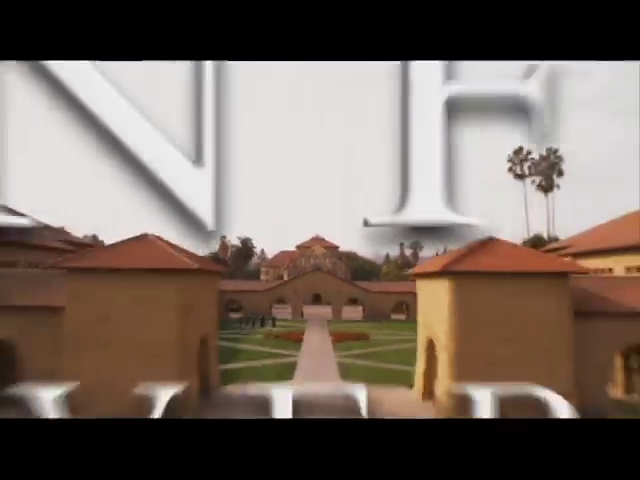
\includegraphics[width=0.78\textwidth]{lecture_02_figure_01.png}
  \caption{Reglas de diferencias finitas y sumas de Riemann que se usarán en el límite continuo posterior.}
  \lectureframe{00:04:20}
  \label{fig:l02-calculus-board}
\end{figure}

Estas son definiciones conocidas del cálculo. Aquí importa cómo escalan: \(\Delta x_i\) aporta un factor de \(\Delta\sigma\), mientras que una suma aporta un factor inverso al convertirse en integral.

\subsection{Extremos de Dirichlet y de Neumann}

El análisis de Fourier en un intervalo finito comienza por elegir las condiciones en los extremos. Dos opciones aparecerán repetidamente.

\begin{align}
  \text{Dirichlet:}\qquad
  &x(0)=x(\pi)=0,
  \label{eq:l02-dirichlet}\\
  \text{Neumann:}\qquad
  &\left.\partial_\sigma x\right|_{\sigma=0}
   =
   \left.\partial_\sigma x\right|_{\sigma=\pi}
   =0.
  \label{eq:l02-neumann}
\end{align}

Una cuerda de violín sujeta por ambos extremos ilustra el caso de Dirichlet: el desplazamiento se anula en los bordes. Una función de Neumann no tiene por qué anularse allí; su pendiente es cero en cada borde. En la pizarra se ven juntas las dos formas características.

\begin{figure}[H]
  \centering
  \begin{minipage}[t]{0.48\textwidth}
    \centering
    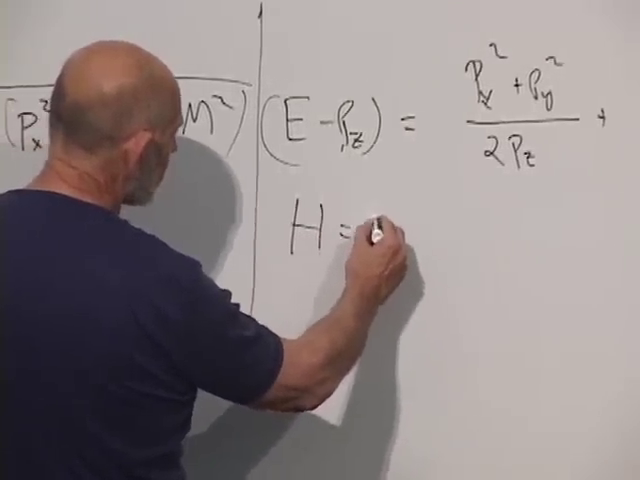
\includegraphics[width=\textwidth]{lecture_02_figure_02.png}
    \par\smallskip\footnotesize (a) Perfiles con extremos fijos y planos.
  \end{minipage}\hfill
  \begin{minipage}[t]{0.48\textwidth}
    \centering
    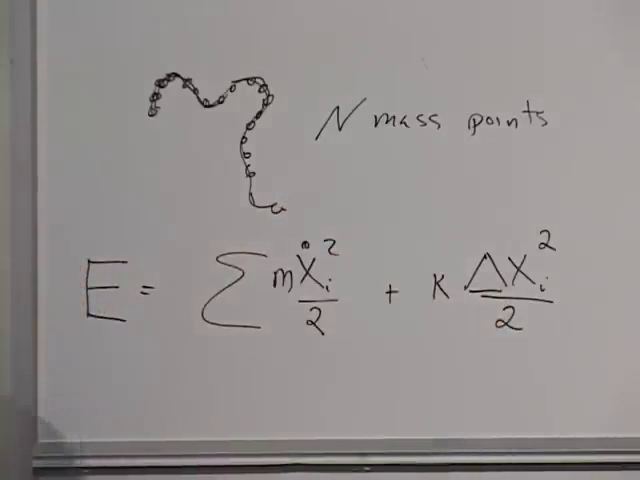
\includegraphics[width=\textwidth]{lecture_02_figure_03.png}
    \par\smallskip\footnotesize (b) Anillos ligeros que se deslizan sobre varillas verticales.
  \end{minipage}
  \caption{Condiciones de contorno representadas como formas y como sistemas mecánicos. El montaje de anillos deslizantes da un movimiento transversal inequívoco a un extremo libre.}
  \lectureframe{00:08:50 and 00:12:15}
  \label{fig:l02-boundaries-board}
\end{figure}

\begin{figure}[H]
  \centering
  \begin{adjustbox}{max width=\linewidth}
  \begin{tikzpicture}[>=Latex,thick,scale=0.92]
    \begin{scope}
      \draw[->] (0,0) -- (4.4,0) node[right] {\(\sigma\)};
      \draw[->] (0,-1.25) -- (0,1.35) node[above] {\(x\)};
      \draw[blue!70!black]
        (0,0) .. controls (0.8,1.1) and (1.4,1.0) .. (2.0,0)
        .. controls (2.7,-1.0) and (3.4,-0.8) .. (4.1,0);
      \fill (0,0) circle (0.06);
      \fill (4.1,0) circle (0.06);
      \node at (2.05,-1.65) {Dirichlet: \(x=0\)};
    \end{scope}
    \begin{scope}[xshift=5.8cm]
      \draw[->] (0,0) -- (4.4,0) node[right] {\(\sigma\)};
      \draw[->] (0,-1.25) -- (0,1.35) node[above] {\(x\)};
      \draw[orange!85!black]
        (0,0.65) .. controls (0.8,0.65) and (1.1,-0.9) .. (2.0,-0.9)
        .. controls (2.9,-0.9) and (3.2,0.55) .. (4.1,0.55);
      \draw[orange!85!black] (0,0.65) -- (0.45,0.65);
      \draw[orange!85!black] (3.65,0.55) -- (4.1,0.55);
      \node at (2.05,-1.65) {Neumann: \(\partial_\sigma x=0\)};
    \end{scope}
  \end{tikzpicture}
  \end{adjustbox}
  \caption{Para los datos de Dirichlet se fija el valor; para los de Neumann, la pendiente.}
  \label{fig:l02-boundaries-redraw}
\end{figure}

\begin{classroomqa}
\audiencequestion{¿Puede un tubo de órgano abierto o cerrado ofrecer un ejemplo claro de alguna de estas condiciones de contorno?\lecturetimestamp{00:09:19}}
\lecturerresponse{Puede, pero primero hay que especificar qué variable acústica se desarrolla. La perturbación de presión y el desplazamiento longitudinal obedecen condiciones idealizadas complementarias en un extremo abierto. En lugar de resolver esa cuestión secundaria en la pizarra, usemos el modelo de anillos deslizantes: anillos casi sin masa pueden moverse verticalmente sobre las varillas, de modo que los extremos de la cuerda quedan libres y el caso de Neumann resulta directo.}
\end{classroomqa}

\begin{classroomqa}
\audiencequestion{¿Puede la gráfica subir verticalmente y contener un salto brusco?\lecturetimestamp{00:09:53}}
\lecturerresponse{El análisis de Fourier admite saltos aislados en una función continua a trozos. Una cuerda física impone más restricciones. Un salto desconecta puntos vecinos y hace que la derivada espacial \(\partial_\sigma x\) sea singular en la energía continua que obtendremos más adelante. Por tanto, nos limitaremos a perfiles continuos y diferenciables.}
\end{classroomqa}

\begin{classroomqa}
\audiencequestion{¿Por qué el extremo abierto de un tubo, o cualquier extremo libre, debe satisfacer alguna condición de contorno?\lecturetimestamp{00:11:14}}
\lecturerresponse{El ejemplo acústico depende del campo elegido y dejamos sin resolver esa cuestión en la discusión. El ejemplo mecánico no presenta esa ambigüedad. Un anillo muy ligero puede deslizarse libremente, pero sigue unido al último tramo de cuerda. Deduciremos su condición a partir de la ley de Newton, en vez de darla por supuesta: una aceleración finita en el extremo obliga a que la pendiente se anule.}
\end{classroomqa}

\subsection{Las bases de Fourier}

Una vez fijada la clase de condiciones en los extremos, queda determinada la base de Fourier correspondiente. En \(0\leq\sigma\leq\pi\),

\begin{align}
  x_D(\sigma)
  &=
  \sum_{n=1}^{\infty}x_n\sin(n\sigma),
  \label{eq:l02-dirichlet-series}\\
  x_N(\sigma)
  &=
  \sum_{n=0}^{\infty}x_n\cos(n\sigma).
  \label{eq:l02-neumann-series}
\end{align}

Todos los senos de \eqref{eq:l02-dirichlet-series} se anulan en ambos extremos. Todas las funciones coseno de \eqref{eq:l02-neumann-series} tienen derivada nula en los extremos. Los límites inferiores son distintos por una razón: \(\sin(0\sigma)=0\) no aporta nada, mientras que \(\cos(0\sigma)=1\) es el modo constante, o de frecuencia nula. Este representa el valor medio de una función de Neumann.

\begin{figure}[H]
  \centering
  \begin{minipage}[t]{0.48\textwidth}
    \centering
    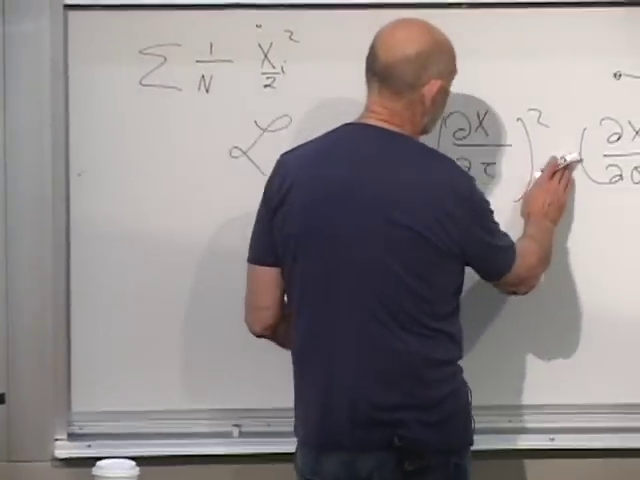
\includegraphics[width=\textwidth]{lecture_02_figure_04.png}
    \par\smallskip\footnotesize (a) Desarrollos en senos y cosenos.
  \end{minipage}\hfill
  \begin{minipage}[t]{0.48\textwidth}
    \centering
    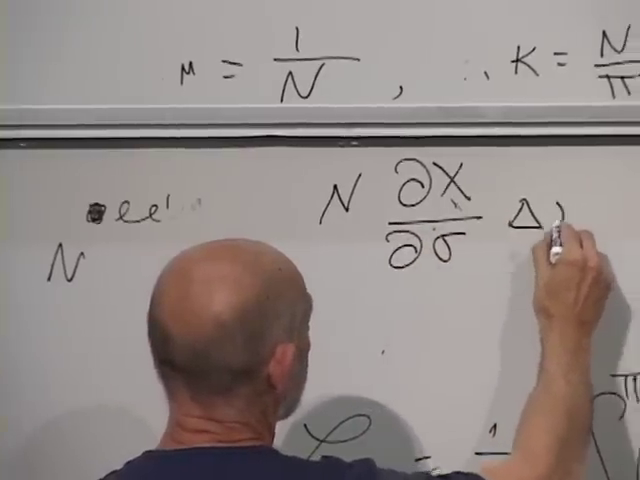
\includegraphics[width=\textwidth]{lecture_02_figure_05.png}
    \par\smallskip\footnotesize (b) Ortogonalidad y el modo constante excepcional.
  \end{minipage}
  \caption{Propiedades de Fourier que usaremos después para diagonalizar la cuerda.}
  \lectureframe{00:16:15 and 00:20:30}
  \label{fig:l02-fourier-board}
\end{figure}

La derivación intercambia las dos clases:

\begin{equation}
  \begin{aligned}
    \partial_\sigma\sin(n\sigma)&=n\cos(n\sigma),\\
    \partial_\sigma\cos(n\sigma)&=-n\sin(n\sigma).
  \end{aligned}
  \label{eq:l02-basis-derivatives}
\end{equation}

Así, la derivada de una serie de Dirichlet tiene comportamiento de Neumann, y la derivada de una serie de Neumann tiene comportamiento de Dirichlet. La ortogonalidad elimina entonces los términos cruzados entre modos distintos:

\begin{align}
  \int_0^\pi\cos(n\sigma)\cos(m\sigma)\,d\sigma
  &=
  \frac{\pi}{2}\delta_{nm},
  && n,m\geq1,
  \label{eq:l02-cos-orthogonality}\\
  \int_0^\pi\sin(n\sigma)\sin(m\sigma)\,d\sigma
  &=
  \frac{\pi}{2}\delta_{nm},
  && n,m\geq1,
  \label{eq:l02-sin-orthogonality}\\
  \int_0^\pi 1\,d\sigma&=\pi .
  \label{eq:l02-zero-norm}
\end{align}

La última línea corresponde a la norma excepcional del coseno \(n=m=0\). Una constante no se normaliza igual que un armónico no nulo, y ese factor de dos distinguirá el modo del centro de masas de la cuerda de sus modos internos.

\subsection{Una fórmula de oscilador para recordar}

Tras reescalar una coordenada para que la masa mecánica sea uno, un oscilador que obedece la ley de Hooke tiene

\begin{align}
  E_{\mathrm{osc}}
  &=
  \frac12\dot q^{\,2}
  +\frac12\omega^2q^2,
  \label{eq:l02-oscillator-energy}\\
  L_{\mathrm{osc}}
  &=
  \frac12\dot q^{\,2}
  -\frac12\omega^2q^2.
  \label{eq:l02-oscillator-lagrangian}
\end{align}

\begin{figure}[H]
  \centering
  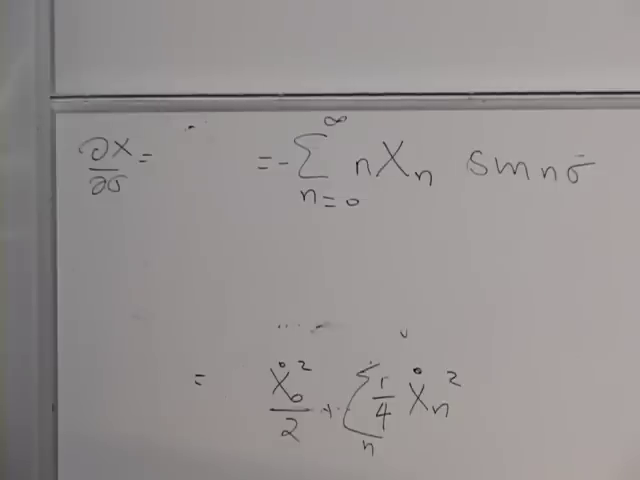
\includegraphics[width=0.68\textwidth]{lecture_02_figure_06.png}
  \caption{La energía del oscilador, escrita de modo que el coeficiente de \(q^2\) permite identificar directamente \(\omega^2\).}
  \lectureframe{00:24:00}
  \label{fig:l02-oscillator-board}
\end{figure}

Clásicamente, \(\omega=\sqrt{\kappa/m}\); el reescalamiento de la coordenada ha fijado \(m=1\). En mecánica cuántica,

\begin{equation}
  E_Q=\hbar\omega\left(Q+\frac12\right),
  \qquad Q=0,1,2,\ldots .
  \label{eq:l02-oscillator-spectrum}
\end{equation}

Para las separaciones entre niveles podemos restar el término común del estado fundamental y decir que cada cuanto cuesta \(\hbar\omega\). El cálculo de la cuerda hará exactamente eso al principio y dejará para más adelante la energía total de punto cero.

\begin{classroomqa}
\audiencequestion{¿Cómo se obtiene la frecuencia del oscilador a partir de la fórmula de la energía?\lecturetimestamp{00:23:21}}
\lecturerresponse{Antes del reescalamiento es \(\omega=\sqrt{\kappa/m}\). Con masa unidad, el término del potencial es \(\frac12\omega^2q^2\), por lo que su coeficiente cuadrático es el cuadrado de la frecuencia.}
\end{classroomqa}

\section{¿Qué hace que un sistema compuesto sea una partícula?}

Una cuerda es extensa y la modelaremos con muchas partes acopladas. ¿En qué sentido puede ser partícula uno de sus estados cuánticos? La puntualidad no puede ser el criterio decisivo. Los protones y los neutrones son compuestos. Los electrones y los fotones están acompañados por el vestido de los campos cuánticos, aunque no se haya resuelto ninguna subestructura intrínseca. La imagen clásica de un punto geométrico rodeado de vacío no es la adecuada para una excitación cuántica.

Tampoco bastan la masa y la posición del centro de masas. Una caja cerrada de gas tiene ambas. Una taza de café también. Normalmente no llamamos partícula a ninguna de las dos. La indivisibilidad tampoco sirve, porque un protón es divisible, y el espín no distingue las partículas microscópicas de los cuerpos macroscópicos.

El criterio útil es el aislamiento espectral. Representemos la energía en reposo en un eje vertical y preguntemos cuánta energía hace falta para llegar a otro estado interno. No hay una sucesión de excitaciones del electrón, accesibles experimentalmente y situadas justo por encima de él. El protón sí tiene resonancias, pero las primeras cuestan unos cientos de MeV, una fracción considerable de la masa del protón. Los estados están lo bastante separados como para identificarlos individualmente.

Una taza de café es lo contrario. Se puede añadir una cantidad arbitrariamente pequeña de energía a un modo sonoro de gran longitud de onda, desplazar una molécula o producir un fonón. Hay cantidades enormes de estados concentrados en un intervalo diminuto. A escala de laboratorio forman un continuo. Esta es la distinción práctica entre una partícula y una \emph{masa informe}.

\begin{figure}[H]
  \centering
  \includegraphics[width=0.58\textwidth]{lecture_02_figure_07.png}
  \caption{Eje vertical de energía en la pizarra al comparar un nivel aislado de una partícula con las numerosas excitaciones de la materia ordinaria.}
  \lectureframe{00:31:10}
  \label{fig:l02-spectrum-board}
\end{figure}

\begin{figure}[H]
  \centering
  \begin{adjustbox}{max width=\linewidth}
  \begin{tikzpicture}[>=Latex,thick]
    \begin{scope}
      \draw[->] (0,0) -- (0,4.8) node[above] {energy};
      \draw[blue!70!black,line width=1.2pt] (-1.0,0.65) -- (1.0,0.65);
      \draw[blue!70!black,line width=1.2pt] (-1.0,3.65) -- (1.0,3.65);
      \node[right] at (1.05,0.65) {ground state};
      \node[right] at (1.05,3.65) {first internal excitation};
      \draw[<->] (0.65,0.75) -- (0.65,3.55)
        node[midway,right] {large gap};
      \node at (0,-0.55) {particle-like};
    \end{scope}
    \begin{scope}[xshift=7.0cm]
      \draw[->] (0,0) -- (0,4.8) node[above] {energy};
      \foreach \y in {0.55,0.69,0.82,0.94,1.05,1.15,1.24,1.32,1.39,1.45,
        1.51,1.57,1.63,1.70,1.78,1.87,1.97,2.09,2.22,2.36,2.51,2.67,2.84,
        3.02,3.21,3.41,3.62,3.84,4.07}
        \draw[orange!85!black] (-0.95,\y) -- (0.95,\y);
      \node[right] at (1.05,2.25) {dense phonon and internal states};
      \node at (0,-0.55) {macroscopic matter};
    \end{scope}
  \end{tikzpicture}
  \end{adjustbox}
  \caption{El criterio operativo de partícula empleado en la lección es el aislamiento espectral, no la puntualidad literal.}
  \label{fig:l02-particle-redraw}
\end{figure}

Este criterio convierte la cuestión filosófica en un cálculo. Cuantizamos la cuerda, hallamos sus niveles de energía interna y examinamos su separación. Si el primer estado excitado de la cuerda está cerca de la escala de Planck mientras que el estado fundamental observado es ligero, la brecha supera en más de veinte órdenes de magnitud las energías actuales de los aceleradores. En el régimen accesible, la cuerda se comporta entonces como una partícula elemental.

\begin{classroomqa}
\audiencequestion{¿El comportamiento de partícula depende únicamente de la escala de observación? Si ampliamos lo suficiente, ¿dejan los niveles de estar separados?\lecturetimestamp{00:33:33}}
\lecturerresponse{Ampliar la imagen puede revelar que un objeto tiene muchos constituyentes, pero no elimina el espectro. La comparación pertinente es entre la resolución energética del experimento y la brecha hasta la primera excitación interna. Un objeto compuesto puede seguir comportándose como una partícula si esa brecha es enorme.}
\end{classroomqa}

\begin{classroomqa}
\audiencequestion{¿Por qué una cuerda de violín ordinaria no es una partícula?\lecturetimestamp{00:34:37}}
\lecturerresponse{La energía de un cuanto vibracional es inconmensurablemente pequeña comparada con la energía en reposo de la cuerda macroscópica. Por tanto, caben muchos estados cuánticos en un intervalo relativo diminuto. La cuerda pertenece al lado denso de la comparación espectral, no al lado aislado.}
\end{classroomqa}

\begin{classroomqa}
\audiencequestion{¿Son partículas puntuales los fotones y los electrones si los campos cuánticos los rodean con fluctuaciones virtuales?\lecturetimestamp{00:35:40}}
\lecturerresponse{La palabra clásica \emph{punto} está cargando con demasiado significado. El electrón y el fotón físicos son excitaciones de campo vestidas; sin embargo, los experimentos no han encontrado en ninguno una estructura intrínseca de constituyentes ni un factor de forma finito. Para el argumento que nos ocupa, lo relevante es que ninguno tiene una densa torre de estados internos casi degenerados.\editorialnote{La conferencia relaciona el momento magnético anómalo del electrón con una borrosidad cuántica medible. En la terminología moderna, el momento anómalo es un efecto de vestidura radiativa, no una prueba de que se haya resuelto un radio finito del electrón. Convencionalmente, «puntual» significa que no se ha detectado subestructura intrínseca ni factor de forma hasta la escala estudiada.}}
\end{classroomqa}

\begin{classroomqa}
\audiencequestion{¿Depende el tamaño de un fotón de su frecuencia?\lecturetimestamp{00:36:49}}
\lecturerresponse{Desde luego, su longitud de onda sí depende de ella. Eso es distinto del tamaño intrínseco de sus constituyentes. Cambiar la frecuencia modifica el paquete de ondas y su longitud de onda, no un radio interno del fotón que se haya podido resolver.}
\end{classroomqa}

\section{Mecánica transversal exacta a gran momento}

Volvamos ahora a la dificultad relativista. No se puede tratar un bastón que gira rápidamente de forma no relativista solo por situar su centro de masas en reposo. Sus extremos siguen moviéndose uno respecto del otro a velocidades relativistas. La aproximación no relativista falla debido al movimiento relativo interno.

Sin embargo, existe otro límite. Elijamos un eje \(z\) y apliquemos un impulso de Lorentz al sistema completo, llevándolo a un momento longitudinal positivo muy grande \(P_z\). Mantengamos finito su momento transversal

\begin{equation}
  p_\perp^2=p_x^2+p_y^2
\end{equation}

 . En el límite \(P_z\to\infty\), la proyección transversal admite entonces una formulación hamiltoniana exactamente no relativista, aunque el movimiento interno sin impulso fuera relativista.

\begin{classroomqa}
\audiencequestion{¿Significa el momento infinito que el sistema masivo alcanza realmente la velocidad de la luz?\lecturetimestamp{00:40:43}}
\lecturerresponse{Ningún impulso finito lo consigue. Se construyen magnitudes con límites bien definidos cuando \(P_z\) crece sin límite. La expresión designa un procedimiento límite, no un estado físico finito con \(v=c\).}
\end{classroomqa}

\begin{classroomqa}
\audiencequestion{¿Qué eje hay que elegir, y qué ocurre si el objeto gira alrededor de ese eje o en torno a otro que lo cruza?\lecturetimestamp{00:41:14}}
\lecturerresponse{Se puede elegir cualquier eje e impulsar el sistema completo a lo largo de él. La mecánica que queda explícita es la de la proyección sobre el plano perpendicular. Una varilla que gira puede parecer acortada o barrer ese plano, pero su proyección transversal tiene forma no relativista.}
\end{classroomqa}

Las cuerdas tienen una propiedad adicional que hace que esta representación sea especialmente potente. En el calibre de frente de luz, las coordenadas longitudinales internas no son osciladores independientes. Las ligaduras las determinan a partir del movimiento transversal. Por tanto, basta conocer la cuerda transversal para reconstruir los grados de libertad físicos.

\begin{classroomqa}
\audiencequestion{¿La ausencia de una coordenada longitudinal independiente significa que la cuerda está simplemente atrapada en un sándwich delgado?\lecturetimestamp{00:42:26}}
\lecturerresponse{La contracción de Lorentz sí hace pequeño su tamaño longitudinal en el sistema de referencia impulsado, pero la afirmación va más allá. Todo movimiento longitudinal residual está condicionado por el movimiento transversal; no se puede especificar de manera independiente.}
\end{classroomqa}

\begin{classroomqa}
\audiencequestion{¿Está relacionada esta reducción a datos transversales con el principio holográfico?\lecturetimestamp{00:43:12}}
\lecturerresponse{Está estrechamente relacionada con la línea de pensamiento que condujo a las ideas holográficas, aunque desarrollar esa conexión nos apartaría del cálculo actual. Aquí solo sirve para justificar que trabajemos con la cuerda transversal.}
\end{classroomqa}

\subsection{Restar el impulso y reescalar el tiempo}

Sea \(M\) la masa invariante del sistema completo, que incluye las masas de los constituyentes, la energía cinética y la energía de enlace. En unidades \(c=1\),

\begin{equation}
  E=\sqrt{P_z^2+p_\perp^2+M^2}.
  \label{eq:l02-relativistic-energy}
\end{equation}

Para valores de \(P_z\) mucho mayores que los de \(p_\perp\) y \(M\),

\begin{equation}
  E
  =
  P_z+\frac{p_\perp^2+M^2}{2P_z}
  +O(P_z^{-3}).
  \label{eq:l02-large-pz}
\end{equation}

\begin{figure}[H]
  \centering
  \includegraphics[width=0.76\textwidth]{lecture_02_figure_08.png}
  \caption{La expansión completa en gran \(P_z\), conservando el momento transversal y la masa invariante.}
  \lectureframe{00:47:30}
  \label{fig:l02-large-pz-board}
\end{figure}

El término dominante es grande, pero no contiene información sobre el estado interno. En un proceso que conserva \(P_z\), como una transición entre niveles internos de un átomo impulsado sin cambiar su momento longitudinal total, ese término se cancela en todas las diferencias de energía. Por tanto, estudiamos

\begin{equation}
  E-P_z=\frac{p_\perp^2+M^2}{2P_z}+O(P_z^{-3}).
  \label{eq:l02-residual-energy}
\end{equation}

El denominador tiene significado físico. Como el hamiltoniano genera la evolución temporal, la pequeña energía residual indica que la evolución interna parece lenta en el tiempo de laboratorio. Esto es la dilatación temporal. Para conservar el movimiento interno, introduzcamos un parámetro de evolución reescalado \(\tau\) o, de forma equivalente, multipliquemos el hamiltoniano residual por \(P_z\):

\begin{equation}
  H_\perp
  \equiv
  \lim_{P_z\to\infty}P_z(E-P_z)
  =
  \frac12p_\perp^2+\frac12M^2.
  \label{eq:l02-transverse-hamiltonian}
\end{equation}

\begin{figure}[H]
  \centering
  \begin{minipage}[t]{0.48\textwidth}
    \centering
    \includegraphics[width=\textwidth]{lecture_02_figure_09.png}
    \par\smallskip\footnotesize (a) \(H=i\partial_t\) y la evolución interna ralentizada.
  \end{minipage}\hfill
  \begin{minipage}[t]{0.48\textwidth}
    \centering
    \includegraphics[width=\textwidth]{lecture_02_figure_10.png}
    \par\smallskip\footnotesize (b) El hamiltoniano transversal finito tras reescalar el tiempo.
  \end{minipage}
  \caption{De la energía residual dilatada en el tiempo a un hamiltoniano finito en dos dimensiones.}
  \lectureframe{00:49:20 and 00:52:40}
  \label{fig:l02-lightfront-board}
\end{figure}

Esta es exactamente la forma de la energía de una partícula de masa unidad que se mueve en dos dimensiones: energía cinética \(p_\perp^2/2\) más energía interna \(M^2/2\). Lo inusual es el cuadrado. En esta descripción, la magnitud que desempeña el papel de la energía en reposo o de enlace es proporcional al cuadrado de la masa invariante.\editorialnote{Con las variables convencionales de frente de luz \(P^\pm=(E\pm P_z)/\sqrt2\), la relación exacta de la capa de masa es \(2P^+P^-=p_\perp^2+M^2\). La ecuación \eqref{eq:l02-transverse-hamiltonian} es la normalización para \(P_z\) grande de la misma relación invariante que se emplea en la lección.}

\begin{classroomqa}
\audiencequestion{¿Qué ocurre con los momentos longitudinales de las partes individuales de un sistema compuesto?\lecturetimestamp{00:51:30}}
\lecturerresponse{Para un objeto compuesto genérico hay que conservar las fracciones del momento longitudinal total \(P_z\) que llevan sus constituyentes. La fórmula anterior utiliza el momento total del centro de masas. La teoría de cuerdas es especial porque sus ligaduras determinan el movimiento longitudinal relativo a partir de los grados de libertad transversales, de modo que no hay que añadir ningún oscilador longitudinal independiente.}
\end{classroomqa}

\section{Una cuerda abierta discreta}

La cuerda impulsada ahora solo se mueve explícitamente en el plano transversal. Denominemos sus dos coordenadas \(X\) y \(Y\), y aproximémosla primero mediante \(N\) puntos materiales unidos por \(N-1\) resortes. Si \(\mu\) es la masa análoga de cada punto y \(k\) la constante del resorte entre vecinos, la energía es

\begin{equation}
  E_N
  =
  \sum_i
  \left[
    \frac{\mu}{2}
    \left(\dot X_i^2+\dot Y_i^2\right)
    +
    \frac{k}{2}
    \left((\Delta X_i)^2+(\Delta Y_i)^2\right)
  \right].
  \label{eq:l02-discrete-energy}
\end{equation}

Cada término en \(X\) tiene un término idéntico en \(Y\), porque el plano transversal tiene dos direcciones. El índice \(i\) identifica un punto de la cadena; no es una coordenada espacial.

\begin{figure}[H]
  \centering
  \begin{minipage}[t]{0.48\textwidth}
    \centering
    \includegraphics[width=\textwidth]{lecture_02_figure_11.png}
    \par\smallskip\footnotesize (a) La cadena de cuentas y su energía discreta.
  \end{minipage}\hfill
  \begin{minipage}[t]{0.48\textwidth}
    \centering
    \includegraphics[width=\textwidth]{lecture_02_figure_12.png}
    \par\smallskip\footnotesize (b) El escalamiento para valores grandes de \(N\) de \(\mu\) y
    \(k\).
  \end{minipage}
  \caption{La cuerda abierta regularizada antes de tomar el límite continuo.}
  \lectureframe{00:57:42 and 01:02:40}
  \label{fig:l02-chain-board}
\end{figure}

\begin{figure}[H]
  \centering
  \begin{adjustbox}{max width=\linewidth}
  \begin{tikzpicture}[>=Latex,thick]
    \foreach \i in {0,...,8} {
      \coordinate (p\i) at ({1.05*\i},{0.30*sin(55*\i)});
      \filldraw[white] (p\i) circle (0.10);
      \draw (p\i) circle (0.10);
    }
    \foreach \i in {0,...,7} {
      \pgfmathtruncatemacro{\j}{\i+1}
      \draw[decorate,decoration={zigzag,segment length=4pt,amplitude=2pt}]
        (p\i) -- (p\j);
    }
    \node[above=0.35cm of p0] {\(i=0\)};
    \node[above=0.35cm of p8] {\(i=N-1\)};
    \draw[<->] (0,-1.15) -- (8.4,-1.15)
      node[midway,below] {\(0\leq\sigma\leq\pi\)};
    \node at (4.2,1.25)
      {\(\mu=1/N,\quad k=N/\pi^2,\quad\Delta\sigma=\pi/N\)};
  \end{tikzpicture}
  \end{adjustbox}
  \caption{Una imagen clara de la regularización. Al refinar la cadena, los puntos se hacen más ligeros y los resortes microscópicos más rígidos.}
  \label{fig:l02-chain-redraw}
\end{figure}

El parámetro \(\sigma\) indica la posición a lo largo de la cadena. Elegir \(0\leq\sigma\leq\pi\) es una convención, no una medición de longitud física. Nos recuerda que la cuerda tiene dos extremos. Más adelante, la cuerda cerrada se parametrizará periódicamente en \(0\leq\sigma<2\pi\).

El límite continuo debe conservar finita la mecánica colectiva. Si la masa de cada cuenta fuera fija, la masa análoga total divergiría; por tanto, elijamos

\begin{equation}
  \mu=\frac{1}{N}.
  \label{eq:l02-mu-scaling}
\end{equation}

Entonces \(N\mu=1\). No es la masa en reposo relativista \(M\); es el coeficiente de inercia del modelo transversal análogo.

Al aumentar su número, los resortes en serie se vuelven más blandos. Para mantener finita la rigidez de la cadena completa, cada resorte microscópico debe hacerse más rígido:

\begin{equation}
  k=\frac{N}{\pi^2}
  =\frac{1}{\pi\,\Delta\sigma}.
  \label{eq:l02-k-scaling}
\end{equation}

Solo es esencial \(k\propto N\). El factor \(\pi^2\) es una normalización elegida para eliminar factores \(\pi\) sobrantes de las fórmulas del continuo.

\begin{classroomqa}
\audiencequestion{¿Es \(\mu\) la masa en reposo física de cada punto de la cuerda?\lecturetimestamp{01:10:34}}
\lecturerresponse{No. Es la masa análoga no relativista que aparece en la cadena transversal. Llamarla \(M\) llevaría a confundirla con la masa invariante en reposo del estado completo de la cuerda relativista. Su única función aquí es producir la inercia continua correcta.}
\end{classroomqa}

\section{El sistema de ondas continuo}

Apliquemos las reglas preparadas al comienzo. Como \(1/N=\Delta\sigma/\pi\),

\begin{align}
  \sum_i\frac{\mu}{2}\dot X_i^2
  &=
  \frac{1}{2\pi}
  \sum_i\dot X_i^2\,\Delta\sigma
  \longrightarrow
  \frac{1}{2\pi}
  \int_0^\pi
  \left(\partial_\tau X\right)^2d\sigma ,
  \label{eq:l02-kinetic-limit}\\
  \sum_i\frac{k}{2}(\Delta X_i)^2
  &\longrightarrow
  \frac{1}{2\pi}
  \int_0^\pi
  \left(\partial_\sigma X\right)^2d\sigma .
  \label{eq:l02-potential-limit}
\end{align}

Para la segunda línea, usemos \(\Delta X_i=\partial_\sigma X\,\Delta\sigma\) junto con \(k=1/(\pi\Delta\sigma)\). El mismo cálculo se aplica a \(Y\).

\begin{figure}[H]
  \centering
  \begin{minipage}[t]{0.48\textwidth}
    \centering
    \includegraphics[width=\textwidth]{lecture_02_figure_13.png}
    \par\smallskip\footnotesize (a) Reemplazos de sumas por integrales y de diferencias por derivadas.
  \end{minipage}\hfill
  \begin{minipage}[t]{0.48\textwidth}
    \centering
    \includegraphics[width=\textwidth]{lecture_02_figure_14.png}
    \par\smallskip\footnotesize (b) La energía continua completa.
  \end{minipage}
  \caption{La cadena discreta se convierte en un campo definido en el intervalo \(\sigma\).}
  \lectureframe{01:05:40 and 01:07:00}
  \label{fig:l02-continuum-board}
\end{figure}

La energía y el lagrangiano resultantes son

\begin{align}
  E
  &=
  \frac{1}{2\pi}
  \int_0^\pi d\sigma\,
  \left[
    (\partial_\tau X)^2+(\partial_\tau Y)^2\right.\notag\\[-0.25em]
  &\hspace{6.5em}\left.
    +(\partial_\sigma X)^2+(\partial_\sigma Y)^2
  \right],
  \label{eq:l02-continuum-energy}\\
  L
  &=
  \frac{1}{2\pi}
  \int_0^\pi d\sigma\,
  \left[
    (\partial_\tau X)^2+(\partial_\tau Y)^2\right.\notag\\[-0.25em]
  &\hspace{6.5em}\left.
    -(\partial_\sigma X)^2-(\partial_\sigma Y)^2
  \right].
  \label{eq:l02-continuum-lagrangian}
\end{align}

\begin{figure}[H]
  \centering
  \includegraphics[width=0.78\textwidth]{lecture_02_figure_15.png}
  \caption{El lagrangiano continuo, con los términos cinético y de estiramiento de signos opuestos.}
  \lectureframe{01:08:48}
  \label{fig:l02-lagrangian-board}
\end{figure}

Si cambiamos el nombre de \(\sigma\) por el de una coordenada espacial ordinaria y llamamos \(X\) al campo \(\phi\), estas son la energía y el lagrangiano de un campo de ondas unidimensional. Al variar \eqref{eq:l02-continuum-lagrangian} se obtiene

\begin{equation}
  \left(\partial_\tau^2-\partial_\sigma^2\right)X=0,
  \qquad
  \left(\partial_\tau^2-\partial_\sigma^2\right)Y=0.
  \label{eq:l02-wave-equation}
\end{equation}

No hace falta resolver directamente estas ecuaciones para el argumento inmediato. Basta con la imagen útil de ondas que viajan a izquierda y derecha a lo largo de la cuerda y se reflejan en los extremos. Una reflexión de Dirichlet invierte el signo del desplazamiento; una de Neumann lo conserva.

\begin{classroomqa}
\audiencequestion{¿Qué significa exactamente la variable temporal \(\tau\)?\lecturetimestamp{01:08:54}}
\lecturerresponse{Es el tiempo reescalado que se usa para seguir el movimiento interno en la descripción de momento longitudinal \(P_z\) grande. Un reloj impulsado junto con el sistema marcha lentamente respecto del tiempo de laboratorio; \(\tau\) elimina esa dilatación para que las oscilaciones internas conserven una frecuencia finita. Para esta mecánica transversal se puede tratar simplemente como el tiempo.\editorialnote{En la lección se llama informalmente tiempo propio a \(\tau\). Para una cuerda extensa, el parámetro preciso de evolución en el frente de luz es un tiempo reescalado y fijado por el calibre, no un único tiempo propio invariante compartido por todos los puntos. El argumento pretendido sobre la dilatación temporal no cambia.}}\end{classroomqa}

Cuando el centro de masas está en reposo en el plano transversal, la parte interna de \eqref{eq:l02-continuum-energy} es proporcional a \(M^2\), con la normalización de \eqref{eq:l02-transverse-hamiltonian}. Por eso, al cuantizar este sistema de ondas aparentemente ordinario aparecerá el espectro relativista de masas.

\begin{classroomqa}
\audiencequestion{¿Tiene nombre \(P_z(E-P_z)\)?\lecturetimestamp{01:11:00}}
\lecturerresponse{Se suele llamar energía de cono de luz o energía de frente de luz. «Frente de luz» describe mejor el plano nulo que se usa como superficie de evolución; la terminología tradicional no es importante para el cálculo.}
\end{classroomqa}

\begin{classroomqa}
\audiencequestion{¿La palabra «cono» se refiere al cono de luz habitual del espacio-tiempo, y fue Dirac quien introdujo esta terminología?\lecturetimestamp{01:11:17}}
\lecturerresponse{La construcción con coordenadas nulas puede dibujarse con ejes a 45 grados, pero la superficie de evolución aquí es un frente de luz, no el cono completo en expansión. Dirac desarrolló formulaciones relacionadas de la dinámica relativista; la cuestión histórica sobre el nombre quedó abierta y no afecta a las ecuaciones.}
\end{classroomqa}

\section{Por qué un extremo libre satisface la condición de Neumann}

Ahora podemos deducir la condición en los extremos en vez de postularla. La ley de Newton es aplicable porque la mecánica transversal impulsada tiene exactamente forma no relativista. Un punto material interior recibe el tirón de resortes a ambos lados. El punto del extremo solo recibe el tirón del resorte que lo une a su vecino.

\begin{classroomqa}
\audiencequestion{¿Por qué podemos usar la ley de Newton al hablar de una cuerda relativista?\lecturetimestamp{01:14:52}}
\lecturerresponse{No estamos aplicando la mecánica newtoniana al movimiento completo en el espacio-tiempo sin impulso. La aplicamos a las variables transversales de la descripción de momento infinito, cuyo hamiltoniano tiene exactamente forma no relativista.}
\end{classroomqa}

En el extremo derecho, la ley de Hooke da, salvo por la orientación,

\begin{equation}
  F_{\mathrm{end}}
  =
  -k\,\Delta X
  =
  -\frac{1}{\pi\Delta\sigma}
   \left(\partial_\sigma X\,\Delta\sigma\right)
  =
  -\frac{1}{\pi}\partial_\sigma X .
  \label{eq:l02-endpoint-force}
\end{equation}

\begin{figure}[H]
  \centering
  \begin{minipage}[t]{0.48\textwidth}
    \centering
    \includegraphics[width=\textwidth]{lecture_02_figure_16.png}
    \par\smallskip\footnotesize Fuerza en el extremo proporcional a la pendiente local.
  \end{minipage}\hfill
  \begin{minipage}[t]{0.48\textwidth}
    \centering
    \includegraphics[width=\textwidth]{lecture_02_figure_17.png}
    \par\smallskip\footnotesize La condición de aceleración finita.
  \end{minipage}
  \caption{Deducción de la condición de contorno en el extremo libre a partir de la ley de Newton.}
  \lectureframe{01:18:20 and 01:20:10}
  \label{fig:l02-neumann-board}
\end{figure}

La ecuación de Newton para el punto del extremo es

\begin{equation}
  \mu\,\partial_\tau^2X=F_{\mathrm{end}},
  \qquad
  \mu=\frac1N=\frac{\Delta\sigma}{\pi}.
  \label{eq:l02-endpoint-newton}
\end{equation}

Combinando \eqref{eq:l02-endpoint-force} y \eqref{eq:l02-endpoint-newton},

\begin{equation}
  \partial_\sigma X
  =
  -\Delta\sigma\,\partial_\tau^2X
  \quad\text{at the right endpoint},
  \label{eq:l02-endpoint-scaling}
\end{equation}

con el signo de la fuerza invertido en el extremo izquierdo. Si \(\partial_\sigma X\) tendiera a una constante distinta de cero cuando \(\Delta\sigma\to0\), la aceleración del extremo divergiría como \(N\). Por tanto, un límite continuo razonable con aceleración finita exige

\begin{equation}
  \left.\partial_\sigma X\right|_{0,\pi}=0,
  \qquad
  \left.\partial_\sigma Y\right|_{0,\pi}=0.
  \label{eq:l02-open-neumann}
\end{equation}

\begin{figure}[H]
  \centering
  \begin{adjustbox}{max width=\linewidth}
  \begin{tikzpicture}[>=Latex,thick,scale=1.0]
    \coordinate (a) at (0,0);
    \coordinate (b) at (4.5,0.75);
    \filldraw[white] (a) circle (0.12);
    \draw (a) circle (0.12);
    \filldraw[white] (b) circle (0.12);
    \draw (b) circle (0.12);
    \draw[decorate,decoration={zigzag,segment length=6pt,amplitude=3pt}]
      (a) -- (b);
    \draw[dashed] (a) -- (0,-1.2);
    \draw[dashed] (b) -- (4.5,-1.2);
    \draw[<->] (4.85,0) -- (4.85,0.75)
      node[midway,right] {\(\Delta X\)};
    \draw[->,red!70!black] (b) -- (5.75,0.95)
      node[right] {\(F_{\rm end}=-k\Delta X\)};
    \node[below] at (0,-1.2) {\(N-1\)};
    \node[below] at (4.5,-1.2) {\(N\)};
    \node at (2.5,-2.0)
      {\(\mu\ddot X=-k\Delta X
      \ \Longrightarrow\
      \partial_\sigma X=-\Delta\sigma\,\ddot X\to0\)};
  \end{tikzpicture}
  \end{adjustbox}
  \caption{En el límite del regulador, la masa del último punto se anula. Solo es posible una aceleración finita si la pendiente en el extremo se anula.}
  \label{fig:l02-neumann-redraw}
\end{figure}

El mismo argumento en ambos extremos y en las dos direcciones transversales da lugar a condiciones de contorno de Neumann para una cuerda abierta libre.

\section{Modos normales de la cuerda abierta}

Ya tenemos un sistema clásico completo: un lagrangiano y sus condiciones de contorno. La cuantización se simplifica tras aplicar el análisis de Fourier. Como los extremos son de Neumann,

\begin{align}
  X(\sigma,\tau)
  &=
  \sum_{n=0}^{\infty}X_n(\tau)\cos(n\sigma),
  \label{eq:l02-X-expansion}\\
  Y(\sigma,\tau)
  &=
  \sum_{n=0}^{\infty}Y_n(\tau)\cos(n\sigma).
  \label{eq:l02-Y-expansion}
\end{align}

Los cosenos contienen toda la dependencia de \(\sigma\). Los coeficientes contienen toda la dependencia temporal; la cuerda oscila porque cambian \(X_n(\tau)\) y \(Y_n(\tau)\).

\begin{figure}[H]
  \centering
  \includegraphics[width=0.78\textwidth]{lecture_02_figure_18.png}
  \caption{La expansión en modos de Neumann, junto a la regla de ortogonalidad que reducirá las sumas dobles.}
  \lectureframe{01:21:45}
  \label{fig:l02-mode-expansion-board}
\end{figure}

\subsection{Término cinético y modo cero}

Al derivar respecto del tiempo, se obtiene

\begin{equation}
  \partial_\tau X
  =
  \sum_{n=0}^{\infty}\dot X_n(\tau)\cos(n\sigma).
  \label{eq:l02-time-mode}
\end{equation}

Al elevar al cuadrado aparece una suma doble sobre \(n\) y \(m\), pero
\eqref{eq:l02-cos-orthogonality} elimina todos los términos con \(n\neq m\).
Separando el modo constante,

\begin{equation}
  \frac{1}{2\pi}\int_0^\pi
  (\partial_\tau X)^2\,d\sigma
  =
  \frac12\dot X_0^{\,2}
  +
  \frac14\sum_{n=1}^{\infty}\dot X_n^{\,2}.
  \label{eq:l02-mode-kinetic}
\end{equation}

\begin{figure}[H]
  \centering
  \includegraphics[width=0.76\textwidth]{lecture_02_figure_19.png}
  \caption{La integral de ortogonalidad reduce la suma doble cinética al modo cero más una suma diagonal.}
  \lectureframe{01:29:10}
  \label{fig:l02-mode-kinetic-board}
\end{figure}

El coeficiente constante es la posición media,

\begin{equation}
  X_0(\tau)=\frac1\pi\int_0^\pi X(\sigma,\tau)\,d\sigma ,
  \label{eq:l02-center-of-mass}
\end{equation}

y, de manera análoga, para \(Y_0\). Con una densidad de masa uniforme análoga, estas son las coordenadas del centro de masas. Tienen energía cinética, pero no fuerza restauradora: toda la cuerda puede moverse libremente por el plano transversal.

\subsection{Término de tensión y frecuencias de los osciladores}

Al derivar respecto de la posición, se obtiene

\begin{equation}
  \partial_\sigma X
  =
  -\sum_{n=1}^{\infty}nX_n(\tau)\sin(n\sigma).
  \label{eq:l02-spatial-mode}
\end{equation}

El modo cero desaparece porque una traslación uniforme no estira la cuerda. Usando la ortogonalidad de los senos,

\begin{equation}
  \frac{1}{2\pi}\int_0^\pi
  (\partial_\sigma X)^2\,d\sigma
  =
  \frac14\sum_{n=1}^{\infty}n^2X_n^{\,2}.
  \label{eq:l02-mode-potential}
\end{equation}

\begin{figure}[H]
  \centering
  \includegraphics[width=0.76\textwidth]{lecture_02_figure_20.png}
  \caption{Al derivar la serie de cosenos se obtiene la suma doble de senos; de nuevo, la ortogonalidad impone \(n=m\).}
  \lectureframe{01:31:40}
  \label{fig:l02-mode-potential-board}
\end{figure}

Por tanto, el lagrangiano del sector \(X\) es

\begin{equation}
  L_X
  =
  \frac12\dot X_0^{\,2}
  +
  \frac14\sum_{n=1}^{\infty}
  \left(
    \dot X_n^{\,2}-n^2X_n^{\,2}
  \right),
  \label{eq:l02-X-lagrangian}
\end{equation}

y para \(Y\) se obtiene una expresión idéntica. La energía correspondiente lleva un signo más delante de \(n^2X_n^2\). Cada modo no nulo es un oscilador armónico independiente, y al comparar con \eqref{eq:l02-oscillator-lagrangian} se obtiene

\begin{equation}
  \omega_n=n,
  \qquad n=1,2,3,\ldots .
  \label{eq:l02-mode-frequency}
\end{equation}

\begin{figure}[H]
  \centering
  \includegraphics[width=0.80\textwidth]{lecture_02_figure_21.png}
  \caption{El lagrangiano de los osciladores desacoplados y la conclusión \(\omega_n=n\), con la torre idéntica de \(Y\) indicada debajo.}
  \lectureframe{01:35:50}
  \label{fig:l02-oscillator-modes-board}
\end{figure}

Los modos normales son simplemente los armónicos de la cuerda. El primero se curva lentamente; el segundo tiene el doble de frecuencia, el tercero el triple, y así sucesivamente. En la teoría libre, la ortogonalidad impide que un armónico se acople a otro.

\begin{classroomqa}
\audiencequestion{¿Qué ocurrió con el oscilador \(n=0\)?\lecturetimestamp{01:34:49}}
\lecturerresponse{Tiene frecuencia cero porque no es en absoluto un oscilador interno. Traslada el centro de masas. Ningún resorte devuelve toda la cuerda a una posición transversal preferida, así que el modo cero es una coordenada de partícula libre.}
\end{classroomqa}

Al omitir el término cinético del centro de masas, queda la energía interna

\begin{equation}
  E_{\mathrm{int}}
  =
  \frac14
  \sum_{n=1}^{\infty}
  \left[
    \dot X_n^{\,2}+n^2X_n^{\,2}
    +\dot Y_n^{\,2}+n^2Y_n^{\,2}
  \right].
  \label{eq:l02-internal-energy}
\end{equation}

En la normalización del frente de luz, esta es proporcional al cuadrado de la masa invariante del estado de la cuerda. Así, hemos convertido el problema relativista de la masa en la mecánica cuántica de dos torres numerables de osciladores.

\section{Niveles cuantizados y comportamiento de partículas}

Sea \(a_n^\dagger\) el operador que crea un cuanto en el oscilador \(X\) de frecuencia \(n\), y sea \(b_n^\dagger\) el que hace lo mismo para \(Y\). La conferencia deja para más adelante un tratamiento sistemático de los operadores, pero esta notación permite ver con claridad el recuento de niveles. Respecto del desplazamiento del estado fundamental,

\begin{equation}
  \begin{aligned}
    \Delta E_{\mathrm{int}}
    &=\sum_{n=1}^{\infty}n\left(Q_n^X+Q_n^Y\right),\\
    Q_n^X,Q_n^Y&\in\{0,1,2,\ldots\}.
  \end{aligned}
  \label{eq:l02-quantized-energy}
\end{equation}

donde \(\hbar=1\). El entero \(n\) indica qué oscilador está excitado; \(Q_n\) cuenta cuántos cuantos lo ocupan.\editorialnote{Cada oscilador también aporta una energía de punto cero. La suma infinita requiere regularización y proporciona el intercepto de la fórmula de la masa de la cuerda. Aquí, la conferencia deja deliberadamente sin especificar el desplazamiento del estado fundamental y cuenta solo los niveles de excitación.}

El vacío de osciladores \(\ket{0}\) no es el espacio-tiempo vacío. Es una cuerda abierta sin ningún oscilador interno excitado. Tiene energía y momento, y ocupa un lugar definido en el espectro de la cuerda.

En el primer nivel hay dos estados,

\begin{equation}
  a_1^\dagger\ket{0},
  \qquad
  b_1^\dagger\ket{0},
  \label{eq:l02-level-one}
\end{equation}

que corresponden al armónico más bajo polarizado a lo largo de \(X\) o de \(Y\). Las combinaciones lineales describen cualquier polarización transversal.

En el segundo nivel hay cinco estados:

\begin{equation}
  (a_1^\dagger)^2\ket{0},
  \quad
  a_1^\dagger b_1^\dagger\ket{0},
  \quad
  (b_1^\dagger)^2\ket{0},
  \quad
  a_2^\dagger\ket{0},
  \quad
  b_2^\dagger\ket{0}.
  \label{eq:l02-level-two}
\end{equation}

Tres contienen dos cuantos del primer armónico; dos contienen un cuanto del segundo armónico. Ambas construcciones cuestan dos unidades.

\begin{figure}[H]
  \centering
  \includegraphics[width=0.76\textwidth]{lecture_02_figure_22.png}
  \caption{Los cinco estados del segundo nivel, enumerados de nuevo tras la pregunta de un asistente: dos excitaciones dobles, una excitación mixta y dos excitaciones del segundo armónico.}
  \lectureframe{01:44:00}
  \label{fig:l02-levels-board}
\end{figure}

\begin{figure}[H]
  \centering
  \begin{adjustbox}{max width=\linewidth}
  \begin{tikzpicture}[>=Latex,thick]
    \draw[->] (0,0) -- (0,5.1) node[above] {\(\Delta E_{\rm int}\)};
    \draw[blue!70!black] (-0.65,0.55) -- (0.65,0.55);
    \node[right] at (0.85,0.55) {\(\ket{0}\) \quad multiplicity \(1\)};
    \draw[blue!70!black] (-0.65,2.15) -- (0.65,2.15);
    \node[right] at (0.85,2.15)
      {\(a_1^\dagger\ket{0},\ b_1^\dagger\ket{0}\)
      \quad multiplicity \(2\)};
    \draw[blue!70!black] (-0.65,3.75) -- (0.65,3.75);
    \node[right,text width=8.6cm] at (0.85,3.75)
      {\((a_1^\dagger)^2\ket{0},
      a_1^\dagger b_1^\dagger\ket{0},
      (b_1^\dagger)^2\ket{0},
      a_2^\dagger\ket{0},\ b_2^\dagger\ket{0}\)
      \quad multiplicity \(5\)};
    \node[left] at (-0.75,0.55) {\(0\)};
    \node[left] at (-0.75,2.15) {\(1\)};
    \node[left] at (-0.75,3.75) {\(2\)};
  \end{tikzpicture}
  \end{adjustbox}
  \caption{Los tres primeros niveles de excitación de la cuerda abierta con dos direcciones transversales.}
  \label{fig:l02-levels-redraw}
\end{figure}

\begin{classroomqa}
\audiencequestion{¿Hay cuatro o cinco estados en el segundo nivel excitado?\lecturetimestamp{01:43:04}}
\lecturerresponse{Cinco. Excitar \(X_1\) dos veces, excitar \(Y_1\) dos veces y excitar cada uno una vez dan tres estados. Excitar \(X_2\) una vez o \(Y_2\) una vez da dos más. El ejercicio propuesto consiste en contar los dos niveles siguientes.}
\end{classroomqa}

La conclusión esencial ya está a la vista. Los niveles sucesivos están separados por brechas finitas y cada uno tiene una multiplicidad finita. Por tanto, según el criterio espectral que la distingue del café, del gas o de una cuerda de violín ordinaria, la cuerda cuantizada se comporta como una partícula. Más adelante determinaremos qué estados son físicamente aceptables y qué patologías deben eliminarse.

\section{Por qué las interacciones de cuerdas abiertas producen cuerdas cerradas}

Una cuerda abierta tiene dos extremos. Sus interacciones elementales unen y dividen cuerdas. En la imagen hadrónica, se puede imaginar un quark en un extremo y un antiquark en el otro; su aniquilación une dos segmentos de cuerda. Las cuerdas fundamentales que nos interesarán más adelante no tienen por qué llevar literalmente esa interpretación hadrónica de sus extremos, pero la regla local de unión se mantiene.

Ahora supongamos que una cuerda abierta fluctúa hasta que sus propios extremos se aproximan. Localmente, un extremo no puede saber si el otro pertenece a la misma cuerda o a otra distinta. Si los extremos pueden unirse, también pueden hacerlo aquí y formar un lazo cerrado.

\begin{figure}[H]
  \centering
  \includegraphics[width=0.70\textwidth]{lecture_02_figure_23.png}
  \caption{Esquema en la pizarra de una cuerda abierta que fluctúa hasta que sus dos extremos se encuentran y forman un lazo cerrado.}
  \lectureframe{01:47:00}
  \label{fig:l02-closed-board}
\end{figure}

\begin{figure}[H]
  \centering
  \begin{adjustbox}{max width=\linewidth}
  \begin{tikzpicture}[>=Latex,thick]
    \begin{scope}
      \draw[blue!70!black]
        (0,0) .. controls (0.8,1.2) and (1.7,-1.0) .. (2.6,0.45)
        .. controls (3.4,1.55) and (4.0,0.3) .. (4.7,0.85);
      \fill (0,0) circle (0.09);
      \fill (4.7,0.85) circle (0.09);
      \node at (2.35,-1.25) {open string fluctuation};
    \end{scope}
    \draw[->,line width=1pt] (5.25,0.3) -- (6.65,0.3)
      node[midway,above] {join};
    \begin{scope}[xshift=8.1cm]
      \draw[orange!85!black]
        (0,0) .. controls (0.3,1.5) and (2.5,1.8) .. (3.1,0.3)
        .. controls (3.5,-1.1) and (0.7,-1.5) .. (0,0);
      \node at (1.55,-1.85) {closed string};
    \end{scope}
  \end{tikzpicture}
  \end{adjustbox}
  \caption{Si se permite que los extremos se unan, una cuerda abierta puede cerrarse sobre sí misma.}
  \label{fig:l02-closed-redraw}
\end{figure}

Así pues, una teoría puede contener cuerdas cerradas sin contener cuerdas abiertas, pero una teoría con interacciones y cuerdas abiertas no puede prescindir de las cuerdas cerradas de manera consistente. Esta asimetría es la predicción importante. Las identificaciones espectrales se desarrollarán más adelante, pero ya se vislumbra el resultado: los estados sin masa de las cuerdas abiertas suelen proporcionar partículas gauge, como los fotones, mientras que el espectro de las cuerdas cerradas contiene un estado sin masa de espín dos: el gravitón. Una vez que la teoría de cuerdas incluye interacciones, las cuerdas cerradas y, por tanto, la gravedad no son un añadido opcional.

\chapter{De los cuantos de cuerda abierta a los taquiones y la gravedad}

\lectureoverview{Ahora cuantizamos los modos normales obtenidos en la clase anterior y preguntamos qué estados de partícula producen. Cada modo transversal es un oscilador armónico, pero su normalización resulta algo poco habitual: excitar el modo \(n\) aumenta la energía de frente de luz y, por tanto, el nivel del cuadrado de la masa, en \(n\) unidades. El primer nivel excitado de la cuerda abierta se transforma exactamente como las dos polarizaciones transversales de un vector sin masa. Por consiguiente, la consistencia relativista fija un valor negativo para el cuadrado de la masa del estado fundamental. Ese estado es el taquión de la cuerda bosónica, cuyo significado real es que el vacío es inestable, no que exista una partícula práctica que viaje más rápido que la luz. Por último, cuando las cuerdas interactúan, la unión y la división hacen inevitables las cuerdas cerradas; la excitación de menor energía de una cuerda cerrada será el gravitón.}

\section{El oscilador oculto en cada modo de la cuerda}

Para una coordenada transversal \(X\), el \(n\) modo normal no nulo tiene la energía y el lagrangiano siguientes:

\begin{align}
  E_n
  &=
  \frac14\dot X_n^{\,2}
  +\frac{n^2}{4}X_n^2,
  \label{eq:l03-mode-energy}\\
  L_n
  &=
  \frac14\dot X_n^{\,2}
  -\frac{n^2}{4}X_n^2.
  \label{eq:l03-mode-lagrangian}
\end{align}

Los factores de \(1/4\) no son un error. Reflejan la normalización elegida al reducir la acción de la cuerda a modos de Fourier independientes. Por tanto, el primer paso para construir el hamiltoniano es calcular el momento canónico:

\begin{equation}
  p_n=\frac{\partial L_n}{\partial\dot X_n}
     =\frac12\dot X_n,
  \qquad
  \dot X_n=2p_n.
  \label{eq:l03-canonical-momentum}
\end{equation}

La transformación de Legendre da

\begin{equation}
  H_n=p_n\dot X_n-L_n
     =p_n^2+\frac{n^2}{4}X_n^2.
  \label{eq:l03-mode-hamiltonian}
\end{equation}

\begin{figure}[H]
  \centering
  \includegraphics[width=0.82\textwidth]{lecture_03_figure_01.png}
  \caption{Energía del modo, lagrangiano, momento canónico y hamiltoniano con la normalización heredada de la cuerda abierta.}
  \lectureframe{00:05:40}
  \label{fig:l03-mode-hamiltonian-board}
\end{figure}

Para factorizar \(H_n\), combinamos \(X_n\) y \(p_n\) así:

\begin{equation}
  \frac{nX_n}{2}\pm i p_n.
\end{equation}

Clásicamente, los dos factores conmutarían, pero en mecánica cuántica

\begin{equation}
  [X_n,p_m]=i\delta_{nm}
  \label{eq:l03-canonical-commutator}
\end{equation}

en unidades en las que \(\hbar=1\). Los términos cruzados no se cancelan sin más. Para un modo fijo:

\begin{align}
  \left[\frac{nX_n}{2}+ip_n,
        \frac{nX_n}{2}-ip_n\right]
  &=n,
  \label{eq:l03-unscaled-commutator}\\
  \left(\frac{nX_n}{2}-ip_n\right)
  \left(\frac{nX_n}{2}+ip_n\right)
  &=H_n-\frac n2.
  \label{eq:l03-factorized-hamiltonian}
\end{align}

\begin{figure}[H]
  \centering
  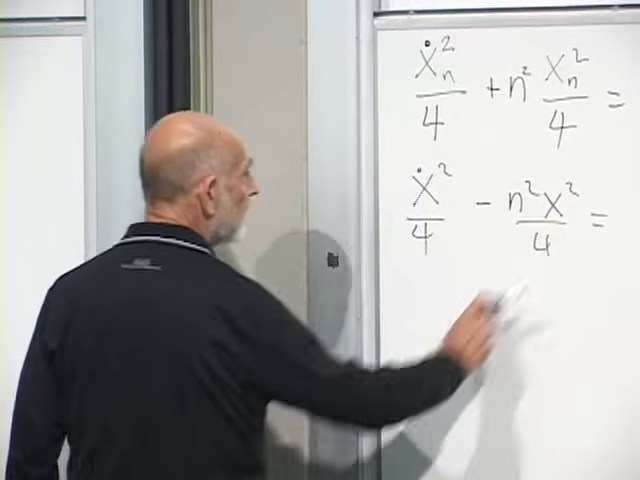
\includegraphics[width=0.82\textwidth]{lecture_03_figure_02.png}
  \caption{El cálculo en la pizarra muestra cómo el conmutador canónico aporta el factor de \(n\).}
  \lectureframe{00:10:30}
  \label{fig:l03-commutator-board}
\end{figure}

El factor de \(n\) nos indica cómo normalizar los operadores escalera:

\begin{align}
  a_n
  &\equiv
  \frac{\sqrt n}{2}X_n+\frac{i}{\sqrt n}p_n,
  \label{eq:l03-annihilator}\\
  a_n^\dagger
  &\equiv
  \frac{\sqrt n}{2}X_n-\frac{i}{\sqrt n}p_n.
  \label{eq:l03-creator}
\end{align}

Satisfacen

\begin{equation}
  [a_n,a_m^\dagger]=\delta_{nm},
  \qquad
  H_n=n\left(a_n^\dagger a_n+\frac12\right).
  \label{eq:l03-oscillator-algebra}
\end{equation}

Así, \(a_n^\dagger\) añade un cuanto del oscilador \(n\), pero ese cuanto lleva \(n\) unidades de energía del modo. No se pierde la separación habitual entre niveles del oscilador; su frecuencia es \(\omega_n=n\).

\begin{figure}[H]
  \centering
  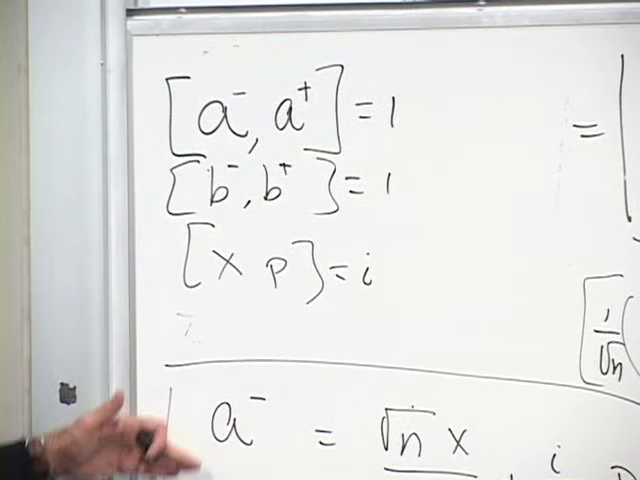
\includegraphics[width=0.82\textwidth]{lecture_03_figure_03.png}
  \caption{Operadores de aniquilación y creación normalizados para el oscilador de cuerda \(n\).}
  \lectureframe{00:12:00}
  \label{fig:l03-ladder-board}
\end{figure}

\subsection{Dos torres transversales}

En cuatro dimensiones espaciotemporales, una cuerda que lleva un momento muy grande a lo largo del eje \(z\) tiene dos coordenadas transversales, \(X\) y \(Y\). Por tanto, necesitamos dos torres independientes de osciladores. Sea \(a_n,a_n^\dagger\) el operador que actúa sobre los modos \(X\) y \(b_n,b_n^\dagger\) el que actúa sobre los modos \(Y\). Al despejar las coordenadas en \eqref{eq:l03-annihilator}--\eqref{eq:l03-creator}, obtenemos

\begin{equation}
  X_n=\frac{a_n+a_n^\dagger}{\sqrt n},
  \qquad
  Y_n=\frac{b_n+b_n^\dagger}{\sqrt n}.
  \label{eq:l03-mode-coordinates}
\end{equation}

\begin{figure}[H]
  \centering
  \includegraphics[width=0.78\textwidth]{lecture_03_figure_04.png}
  \caption{Despeje de la coordenada de un modo en función de sus operadores de creación y aniquilación.}
  \lectureframe{00:17:05}
  \label{fig:l03-coordinate-operator-board}
\end{figure}

Las coordenadas de la cuerda abierta se desarrollaron en modos de Neumann:

\begin{align}
  X(\sigma,\tau)
  &=X_{\rm cm}(\tau)
    +\sum_{n=1}^{\infty}X_n(\tau)\cos(n\sigma),
  \label{eq:l03-X-fourier}\\
  Y(\sigma,\tau)
  &=Y_{\rm cm}(\tau)
    +\sum_{n=1}^{\infty}Y_n(\tau)\cos(n\sigma).
  \label{eq:l03-Y-fourier}
\end{align}

Aparecen cosenos porque las pendientes en los extremos se anulan. Al sustituir \eqref{eq:l03-mode-coordinates}, la propia cuerda se convierte en un operador:

\begin{align}
  X(\sigma,\tau)
  &=X_{\rm cm}(\tau)
    +\sum_{n=1}^{\infty}
      \frac{a_n(\tau)+a_n^\dagger(\tau)}{\sqrt n}
      \cos(n\sigma),
  \label{eq:l03-X-operator}\\
  Y(\sigma,\tau)
  &=Y_{\rm cm}(\tau)
    +\sum_{n=1}^{\infty}
      \frac{b_n(\tau)+b_n^\dagger(\tau)}{\sqrt n}
      \cos(n\sigma).
  \label{eq:l03-Y-operator}
\end{align}

\begin{figure}[H]
  \centering
  \begin{minipage}[t]{0.48\textwidth}
    \centering
    \includegraphics[width=\textwidth]{lecture_03_figure_05.png}
    \par\smallskip\footnotesize (a) Desarrollos de las coordenadas en modos.
  \end{minipage}\hfill
  \begin{minipage}[t]{0.48\textwidth}
    \centering
    \includegraphics[width=\textwidth]{lecture_03_figure_06.png}
    \par\smallskip\footnotesize (b) Sustitución de los operadores escalera en las coordenadas de la cuerda.
  \end{minipage}
  \caption{La forma de la cuerda cuántica abierta se compone de todos sus operadores de oscilador transversales.}
  \lectureframe{00:20:35 and 00:21:05}
  \label{fig:l03-string-coordinate-board}
\end{figure}

\begin{classroomqa}
\audiencequestion{¿Es \(X_n\) también una función de \(\sigma\)?\lecturetimestamp{00:21:48}}
\lecturerresponse{No. Toda la dependencia de \(\sigma\) está en \(\cos(n\sigma)\). El coeficiente \(X_n\) es la amplitud, dependiente del tiempo, de ese patrón espacial, de modo que \(X_n=X_n(\tau)\).}
\end{classroomqa}

\begin{classroomqa}
\audiencequestion{¿Por qué los signos de los operadores llamados de subida y de bajada parecen estar invertidos?\lecturetimestamp{00:23:13}}
\lecturerresponse{El signo visible de \(ip_n\) no determina cómo se nombra el operador. Calculemos el conmutador con el hamiltoniano. El operador que satisface \([H_n,a_n^\dagger]=n a_n^\dagger\) aumenta la energía; el que satisface \([H_n,a_n]=-n a_n\) la disminuye.}
\end{classroomqa}

Las dos torres transversales son una representación pedagógica en cuatro dimensiones. Una cuerda bosónica cuantizada de forma consistente tiene veintiséis dimensiones espaciotemporales, por lo que posee veinticuatro familias de osciladores transversales en vez de dos. El razonamiento que sigue no cambia: el número de estados del primer nivel debe coincidir con el número de polarizaciones físicas de un vector sin masa en la misma dimensión.

\section{Espín masivo y helicidad sin masa}

Antes de asignar espín a los estados de la cuerda, necesitamos establecer una distinción clara. Una partícula masiva de espín \(J\) tiene \(2J+1\) estados de espín:

\begin{equation}
  m_J=-J,-J+1,\ldots,J-1,J.
  \label{eq:l03-massive-spin-multiplet}
\end{equation}

Por ejemplo, una partícula masiva de espín uno tiene tres polarizaciones y una partícula masiva de espín dos tiene cinco. Podemos ver por qué si pasamos al sistema de reposo. Allí están disponibles todas las rotaciones espaciales. Giramos el eje de espín y volvemos a transformar al sistema en movimiento: las \(2J+1\) componentes pertenecen a la misma partícula relativista.

Una partícula sin masa no tiene sistema de reposo. Su etiqueta invariante de espín es la helicidad, el momento angular en la dirección de su movimiento. El fotón solo tiene \(h=+1\) y \(h=-1\); el gravitón solo tiene \(h=+2\) y \(h=-2\). Un escalar tiene un único estado \(h=0\). En la clase se usa la simetría de reflexión para emparejar las dos helicidades. En una teoría quiral, una representación irreducible sin masa puede tener una sola helicidad, así que el emparejamiento es una afirmación adicional sobre la simetría, no una consecuencia de la ausencia de masa por sí sola.\editorialnote{La clasificación moderna mediante el grupo pequeño permite representaciones sin masa de una sola helicidad. La paridad o un contenido de campos que complete adecuadamente la simetría CPT aporta la helicidad opuesta en los ejemplos habituales del fotón y el gravitón.}

\begin{figure}[H]
  \centering
  \begin{minipage}[t]{0.45\textwidth}
    \centering
    \includegraphics[width=\textwidth]{lecture_03_figure_07.png}
    \par\smallskip\footnotesize (a) Recuento de estados de espín iniciado en la pizarra.
  \end{minipage}\hfill
  \begin{minipage}[t]{0.5\textwidth}
    \centering
    \begin{adjustbox}{max width=\linewidth}
    \begin{tabular}{@{}ccc@{}}
      \toprule
      Espín & Estados masivos & Hel icidades sin masa \\
      \midrule
      \(0\) & \(1\) & \(0\) \\
      \(1\) & \(3\) & \(+1,-1\) \\
      \(2\) & \(5\) & \(+2,-2\) \\
      \bottomrule
    \end{tabular}
    \end{adjustbox}
  \end{minipage}
  \caption{La masa elimina el sistema de reposo y, con él, las proyecciones intermedias del espín.}
  \lectureframe{00:27:40}
  \label{fig:l03-spin-count}
\end{figure}

\subsection{Polarización lineal y circular del fotón}

Consideremos un fotón que se mueve a lo largo de \(z\). Sus dos polarizaciones lineales transversales son \(\ket{x}\) y \(\ket{y}\). No son estados propios de helicidad. Los estados de polarización circular son

\begin{align}
  \ket{R}
  &=\frac{1}{\sqrt2}\left(\ket{x}+i\ket{y}\right),
  \label{eq:l03-right-circular}\\
  \ket{L}
  &=\frac{1}{\sqrt2}\left(\ket{x}-i\ket{y}\right),
  \label{eq:l03-left-circular}
\end{align}

con helicidades \(+1\) y \(-1\), según la convención usada para llamar derecha e izquierda a las polarizaciones. Un fotón con polarización lineal es una superposición de esos dos resultados. Su helicidad media puede anularse, pero una medición de helicidad nunca detecta un fotón de espín cero. Asimismo,

\begin{equation}
  \frac{1}{\sqrt2}\left(\ket{x}+\ket{y}\right)
\end{equation}

es simplemente una polarización lineal a cuarenta y cinco grados.

\begin{figure}[H]
  \centering
  \begin{minipage}[t]{0.48\textwidth}
    \centering
    \includegraphics[width=\textwidth]{lecture_03_figure_08.png}
    \par\smallskip\footnotesize (a) Estados de polarización circular en la pizarra.
  \end{minipage}\hfill
  \begin{minipage}[t]{0.48\textwidth}
    \centering
    \begin{adjustbox}{max width=\linewidth}
    \begin{tikzpicture}[>=Latex,scale=0.9]
      \draw[->,thick] (0,0) -- (3.4,0) node[right] {\(z\)};
      \draw[->,blue!70!black,thick] (0,0) -- (0,2.0)
        node[above] {\(x\)};
      \draw[->,orange!85!black,thick] (0,0) -- (-1.4,-1.2)
        node[below left] {\(y\)};
      \draw[red!70!black,thick,->]
        plot[domain=0:320,samples=80]
        ({1.0*cos(\x)},{0.58*sin(\x)+0.4});
      \node[red!70!black] at (1.55,1.25) {circular};
    \end{tikzpicture}
    \end{adjustbox}
  \end{minipage}
  \caption{La polarización lineal proporciona una base transversal; las combinaciones circulares diagonalizan la helicidad.}
  \lectureframe{00:37:45}
  \label{fig:l03-polarization}
\end{figure}

\begin{classroomqa}
\audiencequestion{¿Es esto parecido a la separación de estados de espín en un experimento de Stern--Gerlach?\lecturetimestamp{00:37:40}}
\lecturerresponse{La idea de superposición cuántica es la misma, pero para el fotón el término directo es polarización. Una medición de la polarización circular distingue las dos helicidades; en el haz no hay ningún fotón de espín cero con polarización longitudinal.}
\end{classroomqa}

El gravitón reproduce el patrón con espín dos. Para llevar la cuenta del espín, podemos escribir esquemáticamente

\begin{equation}
  \ket{+2}\sim\ket{+1}\otimes\ket{+1},
  \qquad
  \ket{-2}\sim\ket{-1}\otimes\ket{-1}.
  \label{eq:l03-graviton-helicity}
\end{equation}

Esto no significa que el gravitón esté literalmente compuesto por dos fotones. Significa que dos helicidades iguales se suman para dar la helicidad correcta de espín dos.

\begin{classroomqa}
\audiencequestion{¿La analogía con dos fotones se extiende a otros números cuánticos?\lecturetimestamp{00:41:05}}
\lecturerresponse{No como modelo de constituyentes. Hay fórmulas potentes en las que las amplitudes gravitatorias parecen productos, o ``cuadrados'', de amplitudes de teorías gauge, pero el gravitón sigue siendo una partícula propia. En este caso, la analogía resulta más fiable si se entiende como una afirmación sobre la helicidad.\editorialnote{Las relaciones de Kawai--Lewellen--Tye y las relaciones de doble copia precisan la afirmación sobre las amplitudes en teorías adecuadas; no convierten el gravitón en un estado ligado de dos fotones.}}
\end{classroomqa}

\begin{classroomqa}
\audiencequestion{Un fotón puede tener cualquier momento; ¿no tiene entonces un espectro continuo en vez del espectro discreto que se exige a una partícula?\lecturetimestamp{00:42:17}}
\lecturerresponse{La variable continua es el momento del centro de masas. Fijemos ese momento e inspeccionemos la masa invariante interna. Una partícula se identifica por un nivel de masa discreto; al variar luego su momento total se obtiene la relación de dispersión continua habitual.}
\end{classroomqa}

\section{Los niveles más bajos de la cuerda abierta}

Ahora podemos volver a la cuerda. En la descripción de momento grande, la energía interna finita de frente de luz es proporcional al cuadrado de la masa invariante. Omitiendo la escala global de la cuerda, escribimos el espectro así:

\begin{equation}
  \begin{aligned}
    M^2
    &=m_0^2
      +\sum_{n=1}^{\infty}n
       \left(N_n^{(a)}+N_n^{(b)}\right),\\
    N_n^{(a)}&=a_n^\dagger a_n,
    \qquad
    N_n^{(b)}=b_n^\dagger b_n.
  \end{aligned}
  \label{eq:l03-open-spectrum}
\end{equation}

El estado fundamental del oscilador satisface

\begin{equation}
  a_n\ket{0}=0,
  \qquad
  b_n\ket{0}=0,
  \qquad n=1,2,\ldots .
  \label{eq:l03-ground-annihilation}
\end{equation}

No es una ausencia de cuerda, sino la cuerda cuántica menos excitada, cuyas coordenadas siguen fluctuando. Sea \(m_0^2\) el cuadrado de su masa, aún por determinar.

\begin{figure}[H]
  \centering
  \includegraphics[width=0.78\textwidth]{lecture_03_figure_09.png}
  \caption{El estado fundamental de la cuerda abierta y las condiciones de aniquilación que lo definen.}
  \lectureframe{00:45:20}
  \label{fig:l03-ground-state-board}
\end{figure}

Las excitaciones de menor energía se obtienen usando los operadores de creación \(n=1\):

\begin{equation}
  a_1^\dagger\ket{0},
  \qquad
  b_1^\dagger\ket{0},
  \qquad
  M^2=m_0^2+1.
  \label{eq:l03-first-level}
\end{equation}

\begin{figure}[H]
  \centering
  \includegraphics[width=0.78\textwidth]{lecture_03_figure_10.png}
  \caption{Uno de los dos estados degenerados del primer nivel, con el incremento del cuadrado de la masa escrito en la pizarra.}
  \lectureframe{00:49:25}
  \label{fig:l03-first-level-board}
\end{figure}

El ``uno'' en eqref{eq:l03-first-level} no es un julio, un electronvoltio ni una masa de Planck. Hemos omitido la escala dimensional de cuerdas. Por ahora significa un peldaño en la escalera de masa al cuadrado del oscilador; las unidades que faltan se restablecerán en la próxima clase.

Cualquier combinación lineal de los dos estados degenerados también es un estado de este nivel. En particular,

\begin{equation}
  \frac{1}{\sqrt2}
  \left(a_1^\dagger\pm i b_1^\dagger\right)\ket{0}
  \label{eq:l03-string-circular-states}
\end{equation}

es el análogo de la polarización circular para la cuerda. Bajo una rotación en el plano \(x\)-\(y\), \(a_1^\dagger\) y \(b_1^\dagger\) se transforman como las dos componentes de un vector transversal. Las combinaciones de \eqref{eq:l03-string-circular-states} tienen, por tanto, helicidad \(+1\) y \(-1\).

\begin{figure}[H]
  \centering
  \includegraphics[width=0.82\textwidth]{lecture_03_figure_11.png}
  \caption{Las condiciones del estado fundamental, las dos excitaciones del primer nivel y sus combinaciones circulares, reunidas en la pizarra.}
  \lectureframe{00:56:00}
  \label{fig:l03-level-structure-board}
\end{figure}

No hay un tercer estado degenerado que pueda servir como polarización longitudinal. Si estos dos estados tuvieran masa distinta de cero, una partícula relativista de espín uno necesitaría tres polarizaciones. Al haber exactamente dos, el estado debe ser sin masa. Por tanto,

\begin{equation}
  m_0^2+1=0,
  \qquad
  m_0^2=-1.
  \label{eq:l03-intercept-condition}
\end{equation}

El primer nivel se parece a un fotón: es un estado vectorial gauge sin masa. No tiene por qué ser el fotón del electromagnetismo; su identidad gauge definitiva depende del modelo de cuerda. El estado fundamental que se encuentra por debajo tiene un cuadrado de la masa negativo. Es el taquión de la cuerda bosónica abierta.\editorialnote{En la cuerda bosónica crítica completa, el intercepto de orden normal y el álgebra de Lorentz están ligados a \(D=26\). El cálculo de la clase con dos direcciones transversales es la proyección en cuatro dimensiones del mismo argumento de recuento de estados: los estados de oscilador del primer nivel, \(D-2\), coinciden con las polarizaciones físicas \(D-2\) de un vector sin masa.}

\begin{classroomqa}
\audiencequestion{¿Por qué debería importarnos que \(m_0^2\) sea negativo?\lecturetimestamp{00:56:35}}
\lecturerresponse{Porque el cuadrado de la masa es la curvatura del potencial cuadrático del campo en torno al estado que hemos llamado vacío. Una curvatura negativa significa que esa configuración no es un estado fundamental estable. El siguiente cálculo precisa esta afirmación.}
\end{classroomqa}

\section{Qué significa realmente un taquión}

El nombre ``taquión'' invita a una primera interpretación engañosa. Partamos de la relación de dispersión relativista con \(c=1\):

\begin{equation}
  E(p)=\sqrt{p^2+m^2}.
  \label{eq:l03-relativistic-dispersion}
\end{equation}

Para un paquete de ondas, la velocidad de grupo es

\begin{equation}
  v_g=\frac{dE}{dp}.
  \label{eq:l03-group-velocity}
\end{equation}

Esto reproduce casos conocidos:

\begin{align}
  E_{\rm nr}(p)&=\frac{p^2}{2m},
  &v_g&=\frac{p}{m},
  \label{eq:l03-nr-group-velocity}\\
  E_\gamma(p)&=|p|,
  &|v_g|&=1,
  \label{eq:l03-photon-group-velocity}\\
  E_m(p)&=\sqrt{p^2+m^2},
  &|v_g|&=\frac{|p|}{\sqrt{p^2+m^2}}<1.
  \label{eq:l03-massive-group-velocity}
\end{align}

\begin{figure}[H]
  \centering
  \begin{minipage}[t]{0.48\textwidth}
    \centering
    \includegraphics[width=\textwidth]{lecture_03_figure_12.png}
    \par\smallskip\footnotesize (a) Velocidad de grupo no relativista.
  \end{minipage}\hfill
  \begin{minipage}[t]{0.48\textwidth}
    \centering
    \includegraphics[width=\textwidth]{lecture_03_figure_13.png}
    \par\smallskip\footnotesize (b) Dispersión relativista y su derivada.
  \end{minipage}
  \caption{Obtención de la velocidad de propagación a partir de la pendiente de \(E(p)\).}
  \lectureframe{01:01:50 and 01:03:15}
  \label{fig:l03-group-velocity-board}
\end{figure}

Si \(m^2=-\mu^2\), la expresión formal queda

\begin{equation}
  E(p)=\sqrt{p^2-\mu^2},
  \qquad
  v_g=\frac{p}{\sqrt{p^2-\mu^2}},
  \label{eq:l03-formal-tachyon-dispersion}
\end{equation}

que satisface \(|v_g|>1\) siempre que la raíz cuadrada sea real. Pero esta no es la interpretación física correcta del estado fundamental de la cuerda bosónica. El problema ya aparece a bajo momento, donde la frecuencia es imaginaria.

\subsection{Curvatura negativa del potencial del campo}

Consideremos un campo escalar real en una dimensión espacial:

\begin{equation}
  \left(\partial_t^2-\partial_x^2+m^2\right)\phi=0.
  \label{eq:l03-klein-gordon}
\end{equation}

Para una onda plana \(\phi\propto e^{-i\omega t+ikx}\),

\begin{equation}
  \omega^2=k^2+m^2.
  \label{eq:l03-kg-dispersion}
\end{equation}

\begin{figure}[H]
  \centering
  \includegraphics[width=0.82\textwidth]{lecture_03_figure_14.png}
  \caption{La ecuación de Klein--Gordon usada para poner de manifiesto la inestabilidad que subyace al cuadrado de la masa negativo.}
  \lectureframe{01:06:40}
  \label{fig:l03-klein-gordon-board}
\end{figure}

La energía cuadrática conservada es

\begin{equation}
  \mathcal E
  =\frac12\int dx\,
  \left[
    \dot\phi^{\,2}
    +(\partial_x\phi)^2
    +m^2\phi^2
  \right].
  \label{eq:l03-field-energy}
\end{equation}

\begin{figure}[H]
  \centering
  \includegraphics[width=0.82\textwidth]{lecture_03_figure_15.png}
  \caption{La energía del campo escalar, donde el término de masa determina la curvatura local del potencial.}
  \lectureframe{01:08:10}
  \label{fig:l03-field-energy-board}
\end{figure}

Para \(m^2>0\), el potencial local \(V(\phi)=\tfrac12m^2\phi^2\) tiene forma de cuenco. La configuración \(\phi=0\) está en el fondo. Para \(m^2=-\mu^2\), ese mismo punto se encuentra en la cima de un cuenco invertido. La ecuación \eqref{eq:l03-kg-dispersion} se convierte en

\begin{equation}
  \omega^2=k^2-\mu^2.
  \label{eq:l03-tachyonic-modes}
\end{equation}

Los modos con \(k^2<\mu^2\) tienen

\begin{equation}
  \omega=\pm i\sqrt{\mu^2-k^2},
  \qquad
  \phi_k(t)\propto
  e^{\pm\sqrt{\mu^2-k^2}\,t}.
  \label{eq:l03-growing-mode}
\end{equation}

Una de las ramas crece exponencialmente. Por tanto, el supuesto vacío es inestable: una perturbación de longitud de onda grande, por pequeña que sea, aleja el campo de \(\phi=0\). Eso es lo que significa que haya un taquión en el espectro.

\subsection{La secuencia del péndulo invertido}

Una hilera de péndulos acoplados permite ver la distinción. Coloquemos todos los péndulos en posición vertical. La configuración uniforme existe, pero está en equilibrio en un máximo de energía potencial. Si empujamos un péndulo, cae y tira de sus vecinos. Un frente de péndulos que caen se propaga por la hilera a la velocidad finita de señal que fijan los acoplamientos.

\begin{figure}[H]
  \centering
  \begin{minipage}[t]{0.48\textwidth}
    \centering
    \includegraphics[width=\textwidth]{lecture_03_figure_16.png}
    \par\smallskip\footnotesize (a) El modelo de péndulos verticales acoplados de la pizarra.
  \end{minipage}\hfill
  \begin{minipage}[t]{0.48\textwidth}
    \centering
    \begin{adjustbox}{max width=\linewidth}
    \begin{tikzpicture}[>=Latex,scale=0.78]
      \draw[thick] (-0.3,0) -- (6.3,0);
      \foreach \x/\a in {0/0,1/0,2/8,3/28,4/55,5/72,6/78}{
        \fill (\x,0) circle (0.06);
        \draw[thick] (\x,0) -- ++({90-\a}:1.25);
        \fill[blue!65!black]
          ($(\x,0)+({90-\a}:1.25)$) circle (0.11);
      }
      \draw[red!70!black,->,thick] (1.7,-0.45) -- (4.6,-0.45)
        node[midway,below] {falling front};
    \end{tikzpicture}
    \end{adjustbox}
  \end{minipage}
  \caption{La inestabilidad se propaga causalmente por un sistema aunque su espectro linealizado contenga un cuadrado de la masa negativo.}
  \lectureframe{01:10:40}
  \label{fig:l03-pendulum-instability}
\end{figure}

Nada en este mecanismo permite que una señal controlada se adelante al frente causal. Un modo taquiónico revela un punto de expansión inadecuado, no un mensajero superlumínico estable.\editorialnote{En una ecuación de campo relativista local, la velocidad del frente sigue siendo la velocidad causal. La velocidad de grupo formal de la rama real a alta \(k\) no convierte el vacío inestable en un canal de comunicación más rápido que la luz.}

\begin{classroomqa}¿Es el estado sin masa que acabamos de encontrar el gravitón que predice la teoría de cuerdas?\audiencequestion{\lecturetimestamp{01:14:27}}
\lecturerresponse{No. Es el estado de espín uno de una cuerda abierta con dos polarizaciones, por lo que se parece a un bosón gauge. El gravitón es una excitación de espín dos de una cuerda cerrada.}
\end{classroomqa}

\begin{classroomqa}¿Es matemáticamente admisible un potencial invertido y dónde acabaría el sistema después de caer?\audiencequestion{\lecturetimestamp{01:15:17}}
\lecturerresponse{Es una aproximación local perfectamente legítima, pero por sí sola no tiene estado fundamental porque la energía no está acotada inferiormente. Un potencial más completo puede volver a curvarse hacia arriba y tener un mínimo más bajo. Entonces el sistema rueda o condensa hacia esa configuración estable.}
\end{classroomqa}

La cuerda bosónica ordinaria tiene precisamente este defecto. Sus estados de oscilador de mayor energía siguen formando parte del espectro, pero son excitaciones de un fondo inestable. Las teorías de supercuerdas consistentes eliminan el taquión de cuerda abierta en sus sectores estables, a la vez que conservan excitaciones de cuerda sin masa y masivas.

\begin{classroomqa}¿Las demás propiedades del estado de cuerda abierta coinciden con las de un fotón tanto como coinciden sus dos polarizaciones?\audiencequestion{\lecturetimestamp{01:17:07}}
\lecturerresponse{El estado se comporta como un bosón gauge sin masa. Sus asignaciones de carga, reglas de radiación e identidad detalladas dependen del modelo de cuerda, así que conviene llamarlo parecido a un fotón en vez de identificarlo de inmediato con el electromagnetismo. Las interacciones correspondientes se desarrollarán más adelante.}
\end{classroomqa}

\section{Cómo interactúan las cuerdas}

El espectro libre es solo la mitad de la teoría. Las cuerdas también se unen y se dividen. Conviene recordar primero que una cuerda libre excitada puede llevar momento angular. Una cuerda recta en rotación gira alrededor de su centro de masas, y su energía y su momento angular aumentan juntos siguiendo la trayectoria característica de las cuerdas.

\begin{figure}[H]
  \centering
  \includegraphics[width=0.72\textwidth]{lecture_03_figure_17.png}
  \caption{Esquema de una cuerda abierta que gira alrededor de su centro de masas.}
  \lectureframe{01:19:30}
  \label{fig:l03-rotating-string-board}
\end{figure}

\begin{classroomqa}¿Puede una cuerda libre girar de extremo a extremo alrededor de un extremo fijo?\audiencequestion{\lecturetimestamp{01:20:02}}
\lecturerresponse{No, si no está anclada. Un sistema libre y aislado gira alrededor de su centro de masas. Si un extremo está unido a otro objeto o a una brana, el sistema conjunto puede girar alrededor de otro centro, igual que un electrón y un núcleo orbitan en torno a su centro de masas común mientras el núcleo, mucho más pesado, parece casi inmóvil.}
\end{classroomqa}

\subsection{El vértice de cuerda abierta}

En las cuerdas abiertas, la interacción elemental ocurre cuando dos extremos coinciden en el mismo punto del espacio-tiempo. Hay una amplitud \(g_s\) para que se unan y formen una sola cuerda. Si invertimos la evolución, obtenemos una amplitud para que una cuerda se divida en dos. Esquemáticamente:

\begin{equation}
  \text{open}+\text{open}
  \quad\rightleftarrows\quad
  \text{open}.
  \label{eq:l03-open-joining}
\end{equation}

\begin{figure}[H]
  \centering
  \begin{minipage}[t]{0.48\textwidth}
    \centering
    \includegraphics[width=\textwidth]{lecture_03_figure_18.png}
    \par\smallskip\footnotesize (a) La evolución de unión en la pizarra.
  \end{minipage}\hfill
  \begin{minipage}[t]{0.48\textwidth}
    \centering
    \begin{tikzpicture}[>=Latex,scale=0.9]
      \draw[->] (0,-2.1) -- (0,2.2) node[above] {time};
      \draw[blue!70!black,thick] (-2,-1.6) .. controls (-1.3,-0.9)
        and (-0.7,-0.35) .. (0,0);
      \draw[blue!70!black,thick] (2,-1.6) .. controls (1.3,-0.9)
        and (0.7,-0.35) .. (0,0);
      \draw[orange!85!black,thick] (0,0) .. controls (0.25,0.7)
        and (-0.15,1.25) .. (0.15,1.9);
      \fill[red!70!black] (0,0) circle (0.09);
      \node[right] at (0.12,0) {\(g_s\)};
    \end{tikzpicture}
  \end{minipage}
  \caption{La unión de extremos es el análogo, para las cuerdas, de un vértice de interacción local entre partículas; la inversión temporal da la división.}
  \lectureframe{01:24:05}
  \label{fig:l03-open-vertex}
\end{figure}

El acoplamiento es una amplitud. Para un proceso elemental especificado, la probabilidad correspondiente comienza en el orden \(|g_s|^2\), con factores de espacio de fases y de normalización que aporta el cálculo completo. Llamar \(g_s\)``probabilidad'' al acoplamiento es, por tanto, una forma abreviada e informal de expresarse; distinguir entre amplitud y probabilidad evita introducir un cuadrado espurio.

La interacción no depende de si la cuerda externa está vibrando, girando o en algún otro estado de oscilador. Esos estados modifican el elemento de matriz detallado, pero se aplica la misma regla local de unión.

\subsection{Una cuerda abierta puede cerrarse sobre sí misma}

Supongamos que se encuentran los dos extremos de una cuerda abierta. La regla de unión no puede saber que pertenecen a la misma cuerda. Pueden fusionarse y formar un lazo cerrado:

\begin{equation}
  \text{open}\longrightarrow\text{closed}.
  \label{eq:l03-self-closing}
\end{equation}

\begin{figure}[H]
  \centering
  \begin{minipage}[t]{0.48\textwidth}
    \centering
    \includegraphics[width=\textwidth]{lecture_03_figure_19.png}
    \par\smallskip\footnotesize (a) La cuerda abierta acerca sus extremos.
  \end{minipage}\hfill
  \begin{minipage}[t]{0.48\textwidth}
    \centering
    \begin{tikzpicture}[>=Latex,scale=0.92]
      \draw[blue!70!black,thick]
        (-2,0) .. controls (-1.2,1.5) and (1.2,1.5) .. (2,0);
      \fill[red!70!black] (-2,0) circle (0.08);
      \fill[red!70!black] (2,0) circle (0.08);
      \draw[->,thick] (-0.45,-0.45) -- (0.45,-0.45);
      \draw[orange!85!black,thick] (0,-1.55) ellipse (1.15 and 0.58);
      \node at (0,-2.25) {closed string};
    \end{tikzpicture}
  \end{minipage}
  \caption{Las cuerdas abiertas que interactúan generan inevitablemente cuerdas cerradas.}
  \lectureframe{01:27:20}
  \label{fig:l03-open-becomes-closed}
\end{figure}

Esto no es un añadido opcional. Toda teoría de cuerdas abiertas que interactúan debe contener estados de cuerda cerrada. El proceso inverso permite que una cuerda cerrada se abra y se convierta en una cuerda abierta cuando las condiciones de contorno y los extremos permitidos lo admiten.

\begin{classroomqa}Cuando las cuerdas se fusionan o se dividen, ¿cambia su energía de oscilación y determina la teoría cómo ocurre?\audiencequestion{\lecturetimestamp{01:28:05}}
\lecturerresponse{Sí. La energía y el momento se conservan en el proceso completo, mientras que la excitación puede redistribuirse entre las cuerdas salientes. El vértice de interacción y las funciones de onda externas determinan la amplitud de transición.}
\end{classroomqa}

\subsection{Las cuerdas cerradas pueden interactuar sin abrirse}

La implicación es unidireccional. Las cuerdas abiertas que interactúan requieren cuerdas cerradas, pero una teoría puede comenzar solo con cuerdas cerradas. Dos lazos cerrados pueden tocarse, reconectarse y convertirse en un solo lazo cerrado; la evolución inversa divide un lazo en dos. No es necesario que aparezca ningún extremo abierto.

\begin{figure}[H]
  \centering
  \begin{minipage}[t]{0.48\textwidth}
    \centering
    \includegraphics[width=\textwidth]{lecture_03_figure_20.png}
    \par\smallskip\footnotesize (a) Fusión de cuerdas cerradas en la pizarra.
  \end{minipage}\hfill
  \begin{minipage}[t]{0.48\textwidth}
    \centering
    \begin{tikzpicture}[>=Latex,scale=0.88]
      \draw[blue!70!black,thick] (-1.35,0) circle (0.75);
      \draw[blue!70!black,thick] (1.35,0) circle (0.75);
      \draw[->,thick] (-0.35,-1.15) -- (0.35,-1.15);
      \draw[orange!85!black,thick] (0,-2.3) ellipse (1.35 and 0.68);
      \node at (0,1.2) {closed \(+\) closed};
      \node at (0,-3.25) {closed};
    \end{tikzpicture}
  \end{minipage}
  \caption{Las cuerdas cerradas tienen su propia interacción de unión y división y no necesitan pasar por un estado de cuerda abierta.}
  \lectureframe{01:29:05}
  \label{fig:l03-closed-fusion}
\end{figure}

\begin{classroomqa}Si una teoría comienza con cuerdas cerradas, ¿debe contener también cuerdas abiertas?\audiencequestion{\lecturetimestamp{01:28:35}}
\lecturerresponse{No. Las cuerdas cerradas pueden interactuar mediante reconexión y seguir siendo cerradas en todo momento. Las cuerdas abiertas requieren datos de contorno adicionales, como extremos permitidos o branas.}
\end{classroomqa}

\section{Por qué no se puede evitar la gravedad}

El cálculo de los osciladores de la cuerda cerrada es análogo al de la cuerda abierta, pero hay excitaciones independientes que se mueven a izquierda y a derecha. Su primer nivel no trivial con niveles coincidentes contiene un estado sin masa de espín dos. Ese estado tiene las helicidades de un gravitón. Por consiguiente, toda teoría consistente de cuerdas cerradas contiene gravedad.

\begin{classroomqa}
\audiencequestion{¿Por qué la excitación de menor energía de la cuerda cerrada tiene que ser un gravitón, igual que el nivel de la cuerda abierta tenía que ser de tipo fotónico?
\lecturetimestamp{01:30:59}}
\lecturerresponse{La respuesta se basa en el mismo tipo de conteo de estados, ahora con vectores de oscilador de movimiento hacia la izquierda y hacia la derecha. Su producto tensorial contiene una polarización sin masa, simétrica, sin traza y de espín dos. El espectro explícito de la cuerda cerrada se desarrollará en la próxima clase; en esta etapa, lo esencial es que ese estado es inevitable.}
\end{classroomqa}

Las cuerdas abiertas y cerradas también pueden interactuar entre sí. Un lazo cerrado puede encontrarse con una cuerda abierta y ser absorbido, dejando una cuerda abierta más larga o con una excitación distinta. A la inversa, una cuerda abierta puede emitir un lazo cerrado. En términos de partículas, esto corresponde a la emisión o absorción de un gravitón por la materia.

\begin{figure}[H]\centering
  \begin{minipage}[t]{0.48\textwidth}
    \centering
    \includegraphics[width=\textwidth]{lecture_03_figure_21.png}
    \par\smallskip\footnotesize (a) Reconexión local de segmentos de cuerda.
  \end{minipage}\hfill
  \begin{minipage}[t]{0.48\textwidth}
    \centering
    \includegraphics[width=\textwidth]{lecture_03_figure_22.png}
    \par\smallskip\footnotesize (b) Un lazo cerrado se une a una cuerda abierta.
  \end{minipage}
  \caption{Los esquemas de la pizarra ilustran las interacciones entre cuerdas abiertas--y cerradas, así como la posibilidad universal de intercambiar gravitones.}
  \lectureframe{01:33:10 and 01:34:35}
  \label{fig:l03-mixed-interactions-board}
\end{figure}

\begin{figure}[H]
  \centering
  \begin{tikzpicture}[>=Latex,scale=0.88]
    \draw[blue!70!black,thick]
      (-3,-0.5) .. controls (-1.7,-0.1) and (-0.8,0.2) .. (0,0);
    \draw[blue!70!black,thick]
      (0,0) .. controls (0.9,0.3) and (2.0,0.1) .. (3,0.55);
    \draw[orange!85!black,thick] (-0.8,1.55) ellipse (0.75 and 0.45);
    \draw[->,red!70!black,thick] (-0.45,1.15) -- (-0.05,0.35);
    \node[blue!70!black] at (-2.2,-0.95) {open string};
    \node[orange!85!black] at (-0.8,2.25) {closed string};
    \node at (1.75,-0.5) {excited open string};
  \end{tikzpicture}
  \caption{Esquema nítido, sin representación del espacio-tiempo, de la absorción de una cuerda cerrada por una cuerda abierta.}
  \label{fig:l03-mixed-interaction-redraw}
\end{figure}

El gravitón puede acoplarse a todos los estados de cuerda porque toda cuerda lleva energía y momento, y las reglas de unión permiten intercambiar cuerdas cerradas. Este es el origen, en la teoría de cuerdas, de la universalidad de la gravedad.

\begin{classroomqa}\audiencequestion{¿Puede una cuerda cerrada convertirse en abierta, o unirse a una cuerda abierta sin violar la regla de los extremos?\lecturetimestamp{01:31:20}}
\lecturerresponse{En una teoría que contenga ambos sectores, una cuerda cerrada puede unirse a una abierta y cambiar su estado. Que una cuerda cerrada aislada pueda simplemente abrirse depende de que la teoría permita extremos admisibles. La regla local de reconexión sigue siendo la misma.}
\end{classroomqa}

\begin{classroomqa}
\audiencequestion{¿Pueden los lazos cerrados quedar enlazados o anudados de forma permanente?\lecturetimestamp{01:35:10}}
\lecturerresponse{A acoplamiento débil, las cuerdas son casi siempre transparentes: pueden atravesarse unas a otras, salvo cuando actúa la pequeña amplitud de reconexión. Por tanto, un enlace o un nudo puede persistir durante algún tiempo, pero la topología puede cambiar cuando se produce una interacción permitida entre cuerdas.}
\end{classroomqa}

\begin{classroomqa}
\audiencequestion{¿La probabilidad de interacción es independiente del estado o la velocidad de la cuerda?\lecturetimestamp{01:36:09}}
\lecturerresponse{El acoplamiento local es el mismo parámetro, pero la probabilidad total de transición también depende de las funciones de onda y del tiempo que las partes pertinentes permanezcan en contacto. Por lo general, un encuentro rápido ofrece menos tiempo para la interacción que uno lento.}
\end{classroomqa}

\section{La escala y el acoplamiento que aún faltan}

Se han dejado deliberadamente para más adelante dos cuestiones de contabilidad. En primer lugar, \(X\) es una longitud, mientras que \(a_n\) es adimensional, así que la proporcionalidad de \eqref{eq:l03-mode-coordinates} debe incluir una escala de longitud. En segundo lugar, elevar el nivel del oscilador no puede añadir literalmente un número adimensional a una masa física al cuadrado. Al recuperar la longitud de cuerda \(\ell_s\), o, de manera equivalente, la pendiente de Regge \(\alpha'\sim\ell_s^2\), se obtienen las dimensiones que faltan:

\begin{equation}
  M^2\sim\frac{1}{\alpha'}(N-a).
  \label{eq:l03-dimensional-spectrum}
\end{equation}

La convención y la normalización precisas se establecerán en la próxima clase.

\begin{classroomqa}
\audiencequestion{¿Qué determina la unidad de longitud de cuerda y la masa que aporta cada operador de creación?\lecturetimestamp{01:37:03}}
\lecturerresponse{Se ha suprimido una constante dimensional: la escala de cuerda, que suele denotarse por \(\ell_s\) o \(\alpha'\). Los operadores osciladores son adimensionales; las potencias de esa escala convierten el número de nivel en longitud, tensión y masa al cuadrado físicas.}
\end{classroomqa}

El segundo parámetro es el acoplamiento de cuerda \(g_s\). En el tratamiento más sencillo, es un número universal que controla la unión y la separación de cuerdas. En modelos más ricos, los extremos pueden llevar etiquetas distintas y las cuerdas pueden encontrarse en uniones. Una configuración en forma de Y es el análogo, para cuerdas, de tres tubos de flujo que se encuentran; en la antigua imagen hadrónica se asocia con un barión de tres quarks, mientras que un único segmento abierto se asemeja a un mesón de quark--antiquark.

\begin{classroomqa}
\audiencequestion{¿Pueden tener los extremos de distintas cuerdas probabilidades de unión diferentes?\lecturetimestamp{01:39:31}}
\lecturerresponse{El modelo más sencillo utiliza un solo acoplamiento. Las teorías más elaboradas asignan cargas o etiquetas de contorno a los extremos, y las reglas de selección determinan entonces qué uniones están permitidas. La construcción detallada se verá más adelante, pero la idea universal de unión local se mantiene.}
\end{classroomqa}

\begin{classroomqa}
\audiencequestion{¿Puede una cuerda dividirse a lo largo o formar una unión en Y?\lecturetimestamp{01:40:01}}
\lecturerresponse{Algunos sistemas de cuerdas sí admiten uniones. No se trata del proceso ordinario de división de una cuerda con dos extremos que acabamos de dibujar, sino de uniones que aparecen cuando la teoría admite cargas de cuerda compatibles. La analogía entre el tubo de flujo del mesón-- y el del barión es una imagen útil para entender la distinción.}
\end{classroomqa}

\begin{classroomqa}
\audiencequestion{¿Cambiar el número de dimensiones del espacio-tiempo modifica el acoplamiento de interacción?\lecturetimestamp{01:42:25}}
\lecturerresponse{Las dimensiones modifican el espectro, el espacio de fases y los acoplamientos efectivos que se obtienen tras la compactificación. El acoplamiento fundamental de cuerda sigue organizando la expansión perturbativa, pero su manifestación en menos dimensiones depende de la geometría y el volumen de las dimensiones extra.}
\end{classroomqa}

\begin{classroomqa}
\audiencequestion{¿Es la gravedad lo que hace que una cuerda libre se mueva desde el principio?\lecturetimestamp{01:43:17}}
\lecturerresponse{No hace falta ninguna fuerza para mantener el movimiento. La posición y la velocidad iniciales especifican una solución libre; la inercia la mantiene en movimiento. La gravedad u otra fuerza modifica ese movimiento. Preguntar qué causó las condiciones iniciales es una cuestión aparte, ajena a la ecuación local de movimiento.}
\end{classroomqa}

Hemos llegado, por tanto, a tres conclusiones relacionadas. La cuantización de una cuerda abierta produce un vector sin masa en su primer nivel excitado; el estado fundamental bosónico que está por debajo es inestable; y las interacciones introducen inevitablemente cuerdas cerradas, cuyo espectro contiene la gravedad. La siguiente tarea consiste en recuperar la escala que falta y llevar a cabo explícitamente la cuantización de la cuerda cerrada.
\chapter{Cuerdas cerradas, emparejamiento de niveles y dualidad}

\lectureoverview{Una cuerda cerrada admite ondas independientes en sus dos direcciones intrínsecas. Al cuantizarlas, en un primer momento parece que se duplica el fotón de la cuerda abierta, pero la invariancia ante el desplazamiento del origen de la coordenada de la cuerda elimina los estados que solo ocupan uno de los sectores. El primer nivel que sobrevive contiene una partícula sin masa de espín dos. La misma idea de cambiar de descripción abre entonces una pregunta más amplia: cuando varían los acoplamientos, ¿qué significa que un objeto sea fundamental?}

\section{Un generador reservado}

Antes de dibujar una cuerda cerrada, recuperemos un hecho de la mecánica canónica. Supongamos que
\begin{equation}
  L=L(q_i,\dot q_i),
\end{equation}
y definamos el momento conjugado a \(q_i\) mediante
\begin{equation}
  p_i=\frac{\partial L}{\partial\dot q_i}.
\end{equation}
Una transformación continua infinitesimal puede escribirse como
\begin{equation}
  \delta q_i=\epsilon f_i(q),
  \label{eq:l04-infinitesimal-transformation}
\end{equation}
donde \(\epsilon\) es un parámetro pequeño. Si esta transformación es una simetría, el teorema de Noether proporciona una carga conservada. Al dividir el desplazamiento de la coordenada por el parámetro común se obtiene el generador
\begin{equation}
  Q=\sum_i p_i f_i(q)
   =\frac{1}{\epsilon}\sum_i p_i\,\delta q_i.
  \label{eq:l04-noether-charge}
\end{equation}
En mecánica cuántica, \(Q\) es el operador que genera la transformación pequeña correspondiente.

Una rotación en el plano \(xy\) es el ejemplo habitual. Con una elección de orientación,
\begin{equation}
  \delta x=\epsilon y,
  \qquad
  \delta y=-\epsilon x,
\end{equation}
y \eqref{eq:l04-noether-charge} se convierte en el momento angular, salvo por la misma elección de signo. El ejemplo concreto no será importante. Lo que importa es el patrón: el momento contraído con el desplazamiento infinitesimal da el generador.

\begin{figure}[H]
  \centering
  \includegraphics[width=0.76\textwidth]{lecture_04_figure_01.png}
  \caption{El momento canónico y el generador de Noether que retomaremos más adelante para el desplazamiento de la coordenada de la cuerda cerrada.}
  \lectureframe{00:05:00}
  \label{fig:l04-noether-board}
\end{figure}

Pronto encontraremos una simetría cuya coordenada no es un punto del espacio ordinario, sino la etiqueta de los puntos a lo largo de una cuerda. La ecuación
\eqref{eq:l04-noether-charge} queda aquí a mano para ese propósito.

\section{Una coordenada alrededor de un lazo}

Una cuerda cerrada no tiene extremos. Elijamos un parámetro
\begin{equation}
  0\leq \sigma<2\pi
\end{equation}
y, por el momento, marquemos un punto como \(\sigma=0\). El punto diametralmente opuesto es \(\sigma=\pi\); un cuarto de vuelta y tres cuartos de vuelta corresponden a \(\pi/2\) y \(3\pi/2\). La marca establece una convención de coordenadas, pero todavía no una característica física.

\begin{figure}[H]
  \centering
  \begin{minipage}[t]{0.58\textwidth}
    \centering
    \includegraphics[width=\textwidth]{lecture_04_figure_02.png}
    \par\smallskip\footnotesize (a) El lazo marcado en la pizarra.
  \end{minipage}\hfill
  \begin{minipage}[t]{0.37\textwidth}
    \centering
    \begin{adjustbox}{max width=\linewidth}
    \begin{tikzpicture}[scale=0.82]
      \draw[thick]
        (0.1,1.1)
        .. controls (1.0,1.55) and (2.4,1.45) .. (2.9,0.4)
        .. controls (3.25,-0.45) and (2.45,-1.35) .. (1.55,-1.05)
        .. controls (0.65,-1.45) and (-0.35,-1.0) .. (-0.35,-0.05)
        .. controls (-0.35,0.55) and (-0.05,0.9) .. (0.1,1.1);
      \fill (0.1,1.1) circle (1.8pt);
      \node[above] at (0.1,1.12) {\(\sigma=0\)};
      \draw[->,thick] (2.55,0.95) arc[start angle=42,end angle=-25,radius=0.62];
      \node[right] at (3.05,0.55) {increasing \(\sigma\)};
    \end{tikzpicture}
    \end{adjustbox}
    \par\smallskip\footnotesize (b) La orientación intrínseca.
  \end{minipage}
  \caption{Se marca un punto para definir el origen y una flecha fija el sentido en que aumenta \(\sigma\).}
  \lectureframe{00:06:48}
  \label{fig:l04-closed-string-origin}
\end{figure}

La flecha a lo largo del lazo indica una orientación \emph{intrínseca}. No debe confundirse con el movimiento en sentido horario o antihorario en el plano \(xy\). Imaginemos que levantamos de la pizarra una banda elástica marcada, le damos la vuelta y la volvemos a colocar. El sentido horario aparente se invierte, pero la secuencia de sus marcas intrínsecas no. Lo que aumenta en \(\sigma\) sigue aumentando en \(\sigma\).

Esta distinción determina cómo hablamos de ondas que se propagan hacia la derecha y hacia la izquierda. En este capítulo, una perturbación que se propaga hacia la derecha es la que avanza hacia valores crecientes de \(\sigma\), y una que se propaga hacia la izquierda avanza hacia valores decrecientes de \(\sigma\). Ninguno de estos nombres indica en qué sentido parece moverse la perturbación en la sala.

La orientación tenía un papel concreto en el modelo original de cuerdas hadrónicas. Al romperse un tubo de flujo orientado, se produce un quark en un extremo y un antiquark en el otro; la flecha intrínseca distingue ambos extremos. También pueden construirse teorías de cuerdas no orientadas, pero en esta exposición conservaremos la flecha y los dos sentidos a lo largo de ella.

\section{Periodicidad y ondas viajeras}

Sean \(X(\sigma,\tau)\) y \(Y(\sigma,\tau)\) dos coordenadas transversales de la cuerda, y denotemos el tiempo por \(\tau\). Las coordenadas transversales adicionales, si las hay, se tratan exactamente del mismo modo. Puesto que \(\sigma=0\) y \(\sigma=2\pi\) etiquetan el mismo punto,
\begin{equation}
  X(\sigma+2\pi,\tau)=X(\sigma,\tau),
  \qquad
  Y(\sigma+2\pi,\tau)=Y(\sigma,\tau).
  \label{eq:l04-periodicity}
\end{equation}

\begin{figure}[H]
  \centering
  \includegraphics[width=0.76\textwidth]{lecture_04_figure_03.png}
  \caption{Condiciones de contorno periódicas para las dos coordenadas transversales.}
  \lectureframe{00:12:40}
  \label{fig:l04-periodicity-board}
\end{figure}

Por tanto, una ondulación localizada puede circular indefinidamente. Cuando llega a \(2\pi\), reaparece sin más en \(0\). Esto difiere de lo que ocurre en una cuerda abierta, donde una onda viajera llega a un extremo y se refleja: lo que se propagaba hacia la izquierda pasa a propagarse hacia la derecha, y viceversa. Las ondas estacionarias son naturales en una cuerda abierta, mientras que una cuerda cerrada admite dos familias que se propagan de manera independiente.

\subsection{Modos de Fourier complejos}

La base conveniente para una función periódica es
\begin{equation}
  e^{in\sigma}=\cos(n\sigma)+i\sin(n\sigma),
  \qquad n\in\mathbb Z.
\end{equation}
La condición de que el índice sea entero viene impuesta por la periodicidad:
\(e^{in(\sigma+2\pi)}=e^{in\sigma}\). Por ejemplo, sustituir \(n\) por un semientero haría que la función cambiara tras una vuelta completa.

Si por el momento omitimos la dependencia temporal, la expansión en la pizarra es
\begin{align}
  X(\sigma)
  &=
  X_0+
  \sum_{n>0}X_n e^{in\sigma}
  +\sum_{n>0}X_{-n}e^{-in\sigma},
  \label{eq:l04-fourier-x}\\
  Y(\sigma)
  &=
  Y_0+
  \sum_{n>0}Y_n e^{in\sigma}
  +\sum_{n>0}Y_{-n}e^{-in\sigma}.
  \label{eq:l04-fourier-y}
\end{align}
Para \(X\) y \(Y\) reales, en el nivel clásico los coeficientes de índice negativo son los conjugados complejos de los coeficientes de índice positivo. Los modos cero \(X_0\) y \(Y_0\) localizan el centro de masas; son posiciones, no oscilaciones internas.

\begin{figure}[H]
  \centering
  \includegraphics[width=0.82\textwidth]{lecture_04_figure_04.png}
  \caption{Las partes de índices positivo y negativo de la expansión de Fourier periódica, seguidas del modo cero.}
  \lectureframe{00:20:00}
  \label{fig:l04-fourier-board}
\end{figure}

\begin{classroomqa}
\audiencequestion{Si son ondas viajeras, ¿dónde está la coordenada temporal?\lecturetimestamp{00:19:05}}
\lecturerresponse{Solo se ha omitido en la notación de la pizarra. Una solución viajera lleva una fase que depende tanto de \(\sigma\) como de \(\tau\). Con la convención que usaremos más adelante, una familia tiene
\(e^{-in(\tau-\sigma)}\) y la otra
\(e^{-in(\tau+\sigma)}\).}
\end{classroomqa}

Así pues, lo que determina la propagación es la fase completa, no el signo de \(n\) en un factor de Fourier puramente espacial por sí solo. Podemos escribir
\begin{equation}
  X(\sigma,\tau)=X_R(\tau-\sigma)+X_L(\tau+\sigma),
  \label{eq:l04-chiral-solution}
\end{equation}
y, de manera análoga, para \(Y\). Llamar \(R\) a una familia en vez de \(L\) es una convención; el hecho invariante es que hay dos sentidos opuestos a lo largo del círculo de \(\sigma\).\editorialnote{Un factor \(e^{in\sigma}\) en un instante dado no especifica por sí solo una onda viajera. La propagación queda determinada solo cuando se da la fase temporal.}

\section{Energía en los dos sentidos}

La dinámica local es la misma que en la cuerda abierta. Con la normalización simplificada que usamos aquí,
\begin{equation}
  L\propto
  \int_0^{2\pi}d\sigma\,
  \left[
    \dot X^2-X'^2+\dot Y^2-Y'^2
  \right],
  \label{eq:l04-string-lagrangian}
\end{equation}
donde un punto denota \(\partial_\tau\) y una prima denota \(\partial_\sigma\). La energía tiene un signo más entre los términos cinético y elástico:
\begin{equation}
  E\propto
  \int_0^{2\pi}d\sigma\,
  \left[
    \dot X^2+X'^2+\dot Y^2+Y'^2
  \right].
  \label{eq:l04-string-energy}
\end{equation}
Para cualquiera de las dos coordenadas transversales,
\begin{equation}
  \dot X^2+X'^2
  =
  \frac12(\dot X+X')^2+
  \frac12(\dot X-X')^2.
  \label{eq:l04-energy-square-completion}
\end{equation}
Los términos cruzados se cancelan y quedan exactamente las energías cinética y de gradiente originales.

\begin{figure}[H]
  \centering
  \includegraphics[width=0.82\textwidth]{lecture_04_figure_05.png}
  \caption{La energía total reorganizada en los dos sectores de ondas viajeras.}
  \lectureframe{00:25:10}
  \label{fig:l04-energy-board}
\end{figure}

Para \(X_R(\tau-\sigma)\), se cumple \(\dot X_R=-X_R'\); para \(X_L(\tau+\sigma)\), se cumple \(\dot X_L=X_L'\). Por consiguiente, los dos cuadrados de \eqref{eq:l04-energy-square-completion} aíslan las dos familias quirales. Incluyendo todas las coordenadas transversales, definamos
\begin{align}
  E_L&\propto
  \frac12\int_0^{2\pi}d\sigma
  \sum_I(\dot X^I+X^{I\prime})^2,\\
  E_R&\propto
  \frac12\int_0^{2\pi}d\sigma
  \sum_I(\dot X^I-X^{I\prime})^2.
  \label{eq:l04-left-right-energies}
\end{align}
Entonces \(E=E_L+E_R\). Como las ecuaciones son lineales en esta etapa, las ondas de los dos sectores se atraviesan sin dispersarse.

\subsection{El doble de osciladores}

Al sustituir la serie de Fourier en \eqref{eq:l04-string-lagrangian}, cada coeficiente de modo no nulo se convierte en un oscilador armónico. Su frecuencia es proporcional a \(|n|\): una longitud de onda menor implica una frecuencia mayor y, por tanto, una energía de excitación más alta. A diferencia de lo que ocurre en la cuerda abierta, cada frecuencia positiva aparece en dos copias que se propagan de manera independiente.

En la pizarra, los operadores de creación polarizados en \(X\) son \(a_n^+\) y \(a_{-n}^+\), y los polarizados en \(Y\) son \(b_n^+\) y \(b_{-n}^+\). Para separar con mayor claridad la creación de la propagación, escribiremos
\begin{equation}
  a_n^\dagger,\quad b_n^\dagger,
  \qquad
  \widetilde a_n^\dagger,\quad\widetilde b_n^\dagger,
  \qquad n>0.
  \label{eq:l04-oscillator-notation}
\end{equation}
Los operadores sin tilde y con tilde crean modos que se propagan en sentidos opuestos sobre la hoja de universo; \(a\) y \(b\) denotan las dos polarizaciones transversales.

\begin{figure}[H]
  \centering
  \includegraphics[width=0.65\textwidth]{lecture_04_figure_06.png}
  \caption{La notación de la pizarra para los operadores de creación duplicados, polarizados en \(X\) y \(Y\).}
  \lectureframe{00:29:10}
  \label{fig:l04-oscillators-board}
\end{figure}

Si \(N_n^{(a)},N_n^{(b)}\) y sus correspondientes operadores con tilde son números de ocupación, los niveles de oscilación en los dos sentidos son, esquemáticamente,
\begin{equation}
  \begin{aligned}
    N&=\sum_{n>0}n\bigl(N_n^{(a)}+N_n^{(b)}+\cdots\bigr),\\
    \widetilde N&=\sum_{n>0}n
      \bigl(\widetilde N_n^{(a)}+\widetilde N_n^{(b)}+\cdots\bigr).
  \end{aligned}
  \label{eq:l04-level-operators}
\end{equation}
Los puntos suspensivos representan las direcciones transversales adicionales.

\section{La conjetura sobre el espectro que falla}

Recordemos el primer nivel de la cuerda abierta. Al actuar sobre el estado fundamental con \(a_1^\dagger\) o \(b_1^\dagger\) se obtienen dos polarizaciones lineales. Sus combinaciones circulares,
\begin{equation}
  c_\pm^\dagger
  =
  \frac{1}{\sqrt2}
  \left(a_1^\dagger\pm i b_1^\dagger\right),
  \label{eq:l04-open-circular}
\end{equation}
tienen helicidad \(h=\pm1\). La ausencia de un estado asociado de helicidad cero es la señal de un vector sin masa en esta descripción elemental en cuatro dimensiones.

Sea \(m_0^2\) la masa al cuadrado del estado fundamental de la cuerda cerrada. Una primera conjetura ingenua consiste en actuar una vez con cualquiera de los operadores de
\begin{equation}
  a_1^\dagger,\quad b_1^\dagger,\quad
  \widetilde a_1^\dagger,\quad\widetilde b_1^\dagger.
  \label{eq:l04-naive-one-sided}
\end{equation}
Esto se parece a dos copias del fotón de la cuerda abierta, una por cada sentido de propagación. Sin embargo, a la energía siguiente, la lista sin restricciones no se organiza en multipletes de rotación coherentes. El problema no se resuelve con un tratamiento más elaborado. La premisa de que todo monomio de osciladores es un estado físico es incorrecta.

\subsection{Emparejamiento de niveles: primero, como regla}

La condición física de la cuerda cerrada es
\begin{equation}
  N=\widetilde N,
  \qquad\text{equivalently}\qquad E_L=E_R.
  \label{eq:l04-level-matching}
\end{equation}
Por ahora, tomémosla como un postulado; deduciremos su origen solo después de ver qué consigue.

Todos los estados de \eqref{eq:l04-naive-one-sided} tienen una unidad de energía en un sector y ninguna en el otro, de modo que quedan excluidos. Los primeros estados que sobreviven contienen un oscilador de cada familia:
\begin{align}
  a_1^\dagger\widetilde a_1^\dagger\ket{0},
  &\qquad
  b_1^\dagger\widetilde b_1^\dagger\ket{0},
  \label{eq:l04-four-matched-a}\\
  a_1^\dagger\widetilde b_1^\dagger\ket{0},
  &\qquad
  b_1^\dagger\widetilde a_1^\dagger\ket{0}.
  \label{eq:l04-four-matched-b}
\end{align}
Su energía total de oscilación es dos, repartida por igual entre los dos sentidos. Un único operador de creación \(n=2\) tiene la misma energía total de oscilación, pero no satisface \eqref{eq:l04-level-matching}: aporta dos unidades a un solo lado.

\begin{figure}[H]
  \centering
  \includegraphics[width=0.70\textwidth]{lecture_04_figure_07.png}
  \caption{Los cuatro estados del primer nivel que sobreviven al emparejamiento de niveles. En la pizarra se usan los subíndices \(1\) y \(-1\) donde \eqref{eq:l04-four-matched-a}--\eqref{eq:l04-four-matched-b} usa operadores sin tilde y con tilde.}
  \lectureframe{00:41:05}
  \label{fig:l04-level-matched-board}
\end{figure}

\section{Un gravitón en el primer nivel emparejado}

Expresemos las dos familias quirales en una base circular:
\begin{equation}
  c_\pm^\dagger
  =\frac{a_1^\dagger\pm i b_1^\dagger}{\sqrt2},
  \qquad
  \widetilde c_\pm^\dagger
  =\frac{\widetilde a_1^\dagger\pm i\widetilde b_1^\dagger}{\sqrt2}.
  \label{eq:l04-closed-circular}
\end{equation}
Cada factor aporta una helicidad \(+1\) o \(-1\) en el espacio transversal ordinario. Por tanto, sus productos dan
\begin{center}
\begin{tabular}{c c}
  \toprule
  Estado & Hel icidad \\
  \midrule
  \(c_+^\dagger\widetilde c_+^\dagger\ket0\) & \(+2\) \\
  \(c_-^\dagger\widetilde c_-^\dagger\ket0\) & \(-2\) \\
  \(c_+^\dagger\widetilde c_-^\dagger\ket0\) & \(0\) \\
  \(c_-^\dagger\widetilde c_+^\dagger\ket0\) & \(0\) \\
  \bottomrule
\end{tabular}
\end{center}

\begin{classroomqa}
\audiencequestion{¿El segundo factor de polarización circular debe provenir del sector de propagación opuesto?\lecturetimestamp{00:43:20}}
\lecturerresponse{Sí. La primera expresión escrita en la pizarra se corrigió precisamente por este motivo. Aquí, un estado físico debe emparejar un oscilador que se propaga hacia la derecha con otro que se propaga hacia la izquierda; de lo contrario, no satisface el emparejamiento de niveles. Las helicidades se refieren a la polarización en el espacio transversal, mientras que los dos factores corresponden a sentidos opuestos sobre la hoja de universo.}
\end{classroomqa}

\begin{figure}[H]
  \centering
  \includegraphics[width=0.82\textwidth]{lecture_04_figure_08.png}
  \caption{Los cuatro productos en la base circular tras la corrección de la pizarra, con helicidades \(+2,-2,0,0\).}
  \lectureframe{00:46:10}
  \label{fig:l04-helicity-board}
\end{figure}

Una partícula masiva de espín dos tiene cinco proyecciones del espín,
\begin{equation}
  m=2,1,0,-1,-2.
\end{equation}
El nivel emparejado no contiene estados asociados con \(m=\pm1\). Por tanto, no puede formar un multiplete de espín dos masivo. En cambio, una partícula sin masa de espín dos tiene solo las helicidades \(+2\) y \(-2\). Los productos de igual helicidad son precisamente esos dos estados: las polarizaciones del gravitón.

Quedan dos combinaciones de helicidad cero. En el lenguaje usado en clase, una es el dilatón y la otra el axión. Una descripción covariante de la cuerda bosónica cerrada genérica precisa esta afirmación:
\begin{equation}
  \begin{aligned}
    \alpha_{-1}^{I}\widetilde\alpha_{-1}^{J}\ket{0;k}
    &\longrightarrow
    \underbrace{h_{IJ}}_{\text{symmetric traceless}}
    \oplus
    \underbrace{B_{IJ}}_{\text{antisymmetric}}\\
    &\hspace{2.5em}\oplus
    \underbrace{\Phi}_{\text{trace}}.
  \end{aligned}
  \label{eq:l04-massless-tensor-decomposition}
\end{equation}
Estos son el gravitón, la forma diferencial antisimétrica de dos índices y el dilatón. En cuatro dimensiones, la forma de dos índices puede dualizarse a un pseudoescalar similar a un axión, que es el lenguaje adoptado en la clase.\editorialnote{El segundo estado de helicidad cero es, fundamentalmente, el campo tensorial antisimétrico \(B_{\mu\nu}\) del espectro genérico de cuerdas cerradas. Llamarlo axión corresponde a la descripción dual en cuatro dimensiones.}

En este nivel formal, los tres campos no tienen masa. La compactificación, las proyecciones y la dinámica del fondo pueden alterar cuáles grados de libertad escalares o de dos índices siguen siendo ligeros. El gravitón es distinto: una vez que existe un sector de cuerdas cerradas con interacciones coherentes, su estado sin masa de espín dos es inevitable. Por eso la gravedad emerge de las cuerdas cerradas en vez de añadirse como ingrediente separado.

\section{Por qué deben coincidir los niveles}

Volvamos ahora a la marca en \(\sigma=0\). ¿Es una cuenta física unida al lazo o solo el origen de nuestro parámetro? En una cuerda cerrada ordinaria sin marcar, ningún punto debe ser privilegiado. El estado cuántico debe permanecer inalterado cuando se desplazan a la vez todas las etiquetas.

\subsection{La versión discreta}

Regularicemos el lazo como \(M\) puntos ordenados con coordenadas transversales \((X_i,Y_i)\). Omitamos temporalmente \(Y_i\). Una función de onda en el espacio de configuraciones es
\begin{equation}
  \Psi(X_1,X_2,\ldots,X_M).
\end{equation}
Cambiar qué punto se considera primero da una permutación cíclica:
\begin{align}
  \Psi(X_1,X_2,\ldots,X_M)
  &=
  \Psi(X_2,\ldots,X_M,X_1)\nonumber\\
  &=
  \Psi(X_3,\ldots,X_M,X_1,X_2).
  \label{eq:l04-cyclic-wavefunction}
\end{align}
Esto no es invariancia ante una permutación arbitraria. Por ejemplo, insertar \(X_3\) entre \(X_1\) y \(X_2\) cambia la estructura de adyacencia y, en la práctica, corta y vuelve a conectar la cuerda discretizada. Solo el cambio cíclico común de etiquetas
\begin{equation}
  X_i\longrightarrow X_{i+1}\qquad(\text{mod }M)
  \label{eq:l04-discrete-shift}
\end{equation}
expresa la ausencia de un origen preferido.

\begin{figure}[H]
  \centering
  \includegraphics[width=0.82\textwidth]{lecture_04_figure_09.png}
  \caption{Las identidades cíclicas de la función de onda para una cuerda cerrada discretizada.}
  \lectureframe{00:56:20}
  \label{fig:l04-cyclic-board}
\end{figure}

\subsection{La versión del continuo}

En el límite del continuo \(M\to\infty\), el estado es el funcional de onda
\begin{equation*}
  \Psi[X(\sigma),Y(\sigma)].
\end{equation*}
Un cambio cíclico de etiquetas se convierte en
\begin{equation}
  \sigma\longrightarrow\sigma+\epsilon.
\end{equation}
La invariancia exige que
\begin{equation}
  \Psi[X(\sigma+\epsilon),Y(\sigma+\epsilon)]
  =
  \Psi[X(\sigma),Y(\sigma)].
  \label{eq:l04-wavefunctional-invariance}
\end{equation}

\begin{figure}[H]
  \centering
  \includegraphics[width=0.72\textwidth]{lecture_04_figure_10.png}
  \caption{El desplazamiento discreto y su forma continua como funcional de onda.}
  \lectureframe{00:58:40}
  \label{fig:l04-wavefunctional-board}
\end{figure}

A primer orden,
\begin{equation}
  \delta X(\sigma)=\epsilon X'(\sigma),
  \qquad
  \delta Y(\sigma)=\epsilon Y'(\sigma),
  \label{eq:l04-profile-shift}
\end{equation}
salvo el signo global que distingue un desplazamiento activo del perfil de un desplazamiento pasivo de la coordenada. La variación correspondiente del funcional de onda es
\begin{equation}
  \delta\Psi
  =
  \epsilon\int_0^{2\pi}d\sigma
  \left[
    \frac{\delta\Psi}{\delta X(\sigma)}X'(\sigma)
    +
    \frac{\delta\Psi}{\delta Y(\sigma)}Y'(\sigma)
  \right].
  \label{eq:l04-functional-variation}
\end{equation}

\begin{figure}[H]
  \centering
  \includegraphics[width=0.72\textwidth]{lecture_04_figure_11.png}
  \caption{La expansión a primer orden del argumento desplazado del funcional de onda.}
  \lectureframe{01:01:31}
  \label{fig:l04-functional-expansion-board}
\end{figure}

\begin{classroomqa}
\audiencequestion{¿La condición de primer orden es una ecuación independiente para cada valor de \(\sigma\)?\lecturetimestamp{01:01:30}}
\lecturerresponse{No. La transformación desplaza todos los puntos de la cuerda a la vez. Hay que sumar la variación en un punto a las variaciones en todos los demás; por eso la expresión continua contiene la integral sobre \(\sigma\).}
\end{classroomqa}

En la representación de coordenadas,
\begin{equation}
  P_X(\sigma)=-i\frac{\delta}{\delta X(\sigma)},
  \qquad
  P_Y(\sigma)=-i\frac{\delta}{\delta Y(\sigma)}
  \label{eq:l04-functional-momenta}
\end{equation}
con \(\hbar=1\). Por tanto, la ecuación \eqref{eq:l04-functional-variation} está generada por
\begin{equation}
  G_\sigma=
  \int_0^{2\pi}d\sigma\,
  \left[
    P_X(\sigma)X'(\sigma)+P_Y(\sigma)Y'(\sigma)
  \right].
  \label{eq:l04-sigma-generator}
\end{equation}
Este es exactamente el esquema de Noether \eqref{eq:l04-noether-charge}: el momento canónico multiplicado por el desplazamiento de la coordenada, sumado sobre todos los grados de libertad. Un estado de cuerda cerrada sin marcar satisface
\begin{equation}
  G_\sigma\ket{\mathrm{phys}}=0.
  \label{eq:l04-physical-generator-condition}
\end{equation}

Con la normalización de \eqref{eq:l04-string-lagrangian},
\(P_I\propto\dot X^I\), por lo que la misma condición se escribe
\begin{equation}
  \int_0^{2\pi}d\sigma
  \sum_I\dot X^I X^{I\prime}=0.
  \label{eq:l04-momentum-constraint}
\end{equation}

\begin{figure}[H]
  \centering
  \includegraphics[width=0.75\textwidth]{lecture_04_figure_12.png}
  \caption{El generador integrado, una vez identificado el momento con la derivada del funcional de onda.}
  \lectureframe{01:05:10}
  \label{fig:l04-generator-board}
\end{figure}

\subsection{El generador es la diferencia de energías}

La suma de las dos expresiones de \eqref{eq:l04-left-right-energies} es la energía total. Su diferencia es
\begin{align}
  E_L-E_R
  &\propto
  \frac12\int_0^{2\pi}d\sigma\sum_I
  \left[
    (\dot X^I+X^{I\prime})^2\right.\nonumber\\[-0.25em]
  &\hspace{7em}\left.
    -(\dot X^I-X^{I\prime})^2
  \right]\\
  &=
  2\int_0^{2\pi}d\sigma\sum_I
  \dot X^I X^{I\prime}.
  \label{eq:l04-energy-difference}
\end{align}
La integral es el generador que debe anular un estado físico. Por tanto,
\begin{equation}
  E_L-E_R=0,
  \qquad\text{or}\qquad
  N-\widetilde N=0.
\end{equation}
El emparejamiento de niveles expresa que el origen de la coordenada \(\sigma\) es inobservable.

\begin{figure}[H]
  \centering
  \includegraphics[width=0.78\textwidth]{lecture_04_figure_13.png}
  \caption{La suma y la diferencia de energías que se muestran juntas al final de la deducción del emparejamiento de niveles.}
  \lectureframe{01:06:40}
  \label{fig:l04-energy-difference-board}
\end{figure}

\begin{classroomqa}
\audiencequestion{¿Por qué las fórmulas mostradas parecen colocar el factor de un medio en lugares distintos?\lecturetimestamp{01:06:28}}
\lecturerresponse{Aquí solo se usa la estructura relativa. Al restablecer una normalización global coherente, aparece el factor de un medio en la identidad de cuadrados completos \eqref{eq:l04-energy-square-completion}. La suma da la energía total, mientras que la diferencia sigue siendo proporcional a \(\int d\sigma\,\dot X X'\). Su anulación y, por tanto, el emparejamiento de niveles, son independientes de esa convención común.}
\end{classroomqa}

La restricción elimina una gran parte del espectro ingenuo de osciladores, y elimina precisamente los estados que no formaban multipletes de partículas coherentes. No elimina el fotón de la cuerda abierta, porque una cuerda abierta no tiene dos sectores independientes que circulen y estén sujetos a esta condición propia de un lazo cerrado. En la cuerda cerrada, deja el gravitón, el dilatón, el estado de tensor antisimétrico o similar a un axión, y los niveles emparejados superiores.\editorialnote{En la cuantización covariante de cuerdas, el emparejamiento de niveles es la condición del modo cero \(L_0-\widetilde L_0=0\), uno de los elementos del sistema de restricciones de la hoja de universo. La deducción de aquí aísla su origen intuitivo: la invariancia ante traslaciones alrededor de la cuerda cerrada.}

\section{Dos sentidos distintos de izquierda y derecha}

Ahora hay dos usos distintos del lenguaje de orientación:
\begin{enumerate}
  \item \(X_R(\tau-\sigma)\) y \(X_L(\tau+\sigma)\) describen la propagación en sentidos opuestos a lo largo del círculo intrínseco \(\sigma\).
  \item \(c_+^\dagger\) y \(c_-^\dagger\) describen la polarización circular en el plano transversal físico \(xy\).
\end{enumerate}
El estado del gravitón que satisface el emparejamiento de niveles contiene un oscilador de cada sentido de propagación sobre la hoja de universo. Sin embargo, esos dos osciladores pueden tener la misma helicidad espaciotemporal, lo que produce \(h=+2\) o \(h=-2\). Confundir estos dos sentidos de izquierda y derecha hace que el espectro parezca contradictorio, aunque no lo sea.

\section{¿Qué significa fundamental?}

Una vez cuantizadas las cuerdas abiertas y cerradas en este nivel elemental, queda una pregunta natural: ¿son las cuerdas los constituyentes últimos o podrían estar hechas, a su vez, de algo más?

\begin{classroomqa}
\audiencequestion{¿Hay pruebas o razones para considerar que las cuerdas son los objetos más fundamentales, sin nada más pequeño por debajo de ellas?\lecturetimestamp{01:10:44}}
\lecturerresponse{No hay una respuesta útil que sea independiente del parámetro. Los grados de libertad que parecen elementales en un régimen pueden volverse pesados, extendidos y aparentemente compuestos en otro. Conviene entender «fundamental» como una afirmación sobre qué variables ofrecen una descripción útil para el acoplamiento considerado.}
\end{classroomqa}

Las cargas eléctricas y magnéticas ofrecen el ejemplo más claro de esta idea. Supongamos que una teoría contiene una carga eléctrica \(e\) y una carga magnética \(g\). La cuerda de Dirac inobservable unida a un monopolo exige que
\begin{equation}
  eg=2\pi n,
  \qquad n\in\mathbb Z.
  \label{eq:l04-dirac-quantization}
\end{equation}
Para las cargas mínimas, \(n=1\). Una partícula cargada que rodea la cuerda de Dirac adquiere entonces una fase \(e^{ieg}=1\), de modo que no es posible detectar la cuerda auxiliar.

\begin{figure}[H]
  \centering
  \begin{minipage}[t]{0.58\textwidth}
    \centering
    \includegraphics[width=\textwidth]{lecture_04_figure_14.png}
    \par\smallskip\footnotesize (a) Cuantización de Dirac en la pizarra.
  \end{minipage}\hfill
  \begin{minipage}[t]{0.36\textwidth}
    \centering
    \begin{adjustbox}{max width=\linewidth}
    \begin{tikzpicture}[scale=0.85]
      \fill (0,0) circle (2.5pt);
      \node[above left] at (0,0) {monopole \(g\)};
      \draw[thick] (0,0) -- (3.0,0);
      \node[below] at (1.5,0) {Dirac string};
      \draw[->,thick] (1.5,0.15) arc[start angle=205,end angle=-145,
        x radius=0.8,y radius=0.55];
      \node[right] at (2.15,0.8) {charge \(e\)};
    \end{tikzpicture}
    \end{adjustbox}
    \par\smallskip\footnotesize (b) El experimento de fase alrededor de la cuerda.
  \end{minipage}
  \caption{La condición de Dirac relaciona inversamente las cargas eléctricas y magnéticas.}
  \lectureframe{01:13:20}
  \label{fig:l04-dirac-board}
\end{figure}

Si \(e\) es pequeño, resulta útil la teoría de perturbaciones ordinaria en las variables eléctricas. Los diagramas de Feynman con vértices eléctricos adicionales quedan cada vez más suprimidos. Pero \eqref{eq:l04-dirac-quantization} hace que \(g\) sea grande, por lo que no resulta útil una expansión diagramática en vértices magnéticos. En términos de los acoplamientos adimensionales habituales,
\begin{equation}
  \alpha_e=\frac{e^2}{4\pi},
  \qquad
  \alpha_m=\frac{g^2}{4\pi},
  \qquad
  \alpha_e\alpha_m=\frac{n^2}{4}.
  \label{eq:l04-dual-couplings}
\end{equation}
Un acoplamiento eléctrico débil corresponde a un acoplamiento magnético fuerte, y viceversa.

El monopolo con acoplamiento fuerte también parece complicado desde la descripción eléctrica. La energía de su campo es grande; está vestido por una nube intensa de fluctuaciones del campo gauge y de pares virtuales con carga magnética. Se comporta como un objeto pesado y extendido, un punto de partida poco apropiado para una serie perturbativa eléctrica. Esto no demuestra que sea menos fundamental. Indica que esa variable elemental es inadecuada para ese régimen.

Imaginemos ahora que aumentamos continuamente \(e\). La condición de cuantización obliga a que \(g\) disminuya. Cerca de la región autodual, ninguna de las dos descripciones es especialmente débil; más allá, las variables magnéticas pueden volverse más simples y ligeras, mientras que los objetos eléctricos quedan fuertemente vestidos. La carga que se considera elemental cambia sin que cambie el contenido físico de la teoría.

\subsection{La pregunta de Wigner}

Esta ambigüedad surgió en cierta ocasión en una discusión sobre si el bosón de Higgs era fundamental o compuesto. Eugene Wigner preguntó repetidamente qué significaba «compuesto». Una distinción propuesta se basaba en la desintegración: quizá un objeto fundamental no puede desintegrarse y uno compuesto sí. Pero un átomo de hidrógeno en su estado fundamental no puede desintegrarse y es claramente compuesto; el protón puede ser estable y el neutrón desintegrarse, pero eso no convierte a uno en elemental y al otro en compuesto en el sentido pretendido. Cada definición sencilla daba lugar a otro contraejemplo.

Gerardus 't Hooft cerró la discusión con un criterio operativo: un objeto es fundamental cuando resulta útil considerarlo fundamental. No es una evasiva. Reconoce que «elemental» identifica las variables en las que la dinámica es sencilla, y que la sencillez puede depender del acoplamiento y del entorno.

\section{Hacia la teoría M}

La teoría de cuerdas materializa este intercambio de papeles de una forma especialmente clara. En un régimen de parámetros, las cuerdas son ligeras y perturbativas, mientras que las D-branas parecen compuestos solitónicos pesados, construidos a partir de grados de libertad de cuerdas. Al variar los parámetros, las D-branas pueden convertirse en los objetos elementales más ligeros, y las configuraciones descritas como cuerdas en el primer régimen pueden reinterpretarse en términos de ellas. Lo que parecía fundamental puede volverse compuesto; lo que parecía compuesto puede volverse fundamental.

La antigua imagen reduccionista sugiere un descenso unidireccional desde los objetos grandes hacia constituyentes más pequeños y, por último, hasta una única capa inferior. La dualidad apunta a algo menos lineal: las descripciones pueden transformarse unas en otras al variar los acoplamientos, sin que un conjunto de variables tenga prioridad en todos los regímenes. Desde esta perspectiva abordaremos el siguiente tema: la teoría M.

Siguen abiertas aquí las preguntas de por qué las dimensiones críticas son veintiséis para la cuerda bosónica y diez para la supercuerda. En vez de resolver todas las cuestiones técnicas antes de avanzar, cambiaremos ahora de perspectiva y preguntaremos cómo puede producir la teoría M la teoría de cuerdas en un límite apropiado.
\chapter{Escalas, cuerdas y veintiséis dimensiones}

\lectureoverview{¿Qué determina la separación entre los niveles del espectro de una cuerda? La respuesta es la tensión, una magnitud con dimensiones de masa al cuadrado. Para las cuerdas fundamentales, esta observación conduce a las unidades de Planck, a la imposibilidad práctica de excitarlas directamente y al inicio del régimen de gravedad intensa. Tras una pausa deliberada, volvemos al estado fundamental de la cuerda bosónica abierta. Regular su energía de punto cero proporciona la vía histórica \emph{sencilla} para llegar a veinticuatro direcciones transversales y, por tanto, a veintiséis dimensiones espaciotemporales.}

\section{La escala que habíamos dejado de lado}

Hasta ahora hemos hablado de cuerdas que vibran y giran sin decir qué significa una unidad de excitación. Podemos imaginar un hadrón como una cuerda y excitar sus osciladores, pero ¿cuánto separa un estado del siguiente? ¿Qué determina esa separación?

En el modelo elemental de cuerda hay un solo parámetro dimensional. Para encontrarlo, empecemos con un muelle estirado ordinario. Si sus extremos están separados una distancia \(\ell\), la ley de Hooke da \begin{equation}
  E_{\mathrm{spring}}=\frac{k\ell^2}{2}.
  \label{eq:l05-hooke}
\end{equation} El factor de un medio lo añadió la clase después de que se escribiera la primera versión. En esta estimación inicial, nada esencial dependerá de esos factores numéricos.

\begin{figure}[H]\centering
  \includegraphics[width=0.72\textwidth]{lecture_05_figure_01.png}\caption{El segmento estirado y su energía potencial según la ley de Hooke.}\lectureframe{00:02:28}\label{fig:l05-hooke-board}\end{figure}

La energía de \eqref{eq:l05-hooke} es no relativista. En la descripción de momento infinito que usamos en las clases anteriores, la energía interna no relativista es proporcional a \(m^2\), no a \(m\). Por tanto, escribimos esquemáticamente \begin{equation}
  m^2\sim k\ell^2,
  \qquad
  m\sim \sqrt{k}\,\ell.
  \label{eq:l05-mass-length}
\end{equation} En el sistema de referencia en reposo de la cuerda, su masa es su energía, así que la segunda relación toma la forma \begin{equation}
  E_{\mathrm{rest}}\sim T_s\ell,
  \qquad
  T_s\equiv\sqrt{k}.
  \label{eq:l05-tension}
\end{equation} El coeficiente \(T_s\) es la tensión de la cuerda: la energía almacenada por unidad de longitud.

\begin{figure}[H]\centering
  \includegraphics[width=0.78\textwidth]{lecture_05_figure_02.png}\caption{La pizarra pasa de \(m^2\sim k\ell^2\) a una masa proporcional a la longitud.}\lectureframe{00:05:42}\label{fig:l05-mass-length-board}\end{figure}

Esta notación se adapta a la analogía del muelle usada en la clase. En la notación relativista estándar para cuerdas suele escribirse \begin{equation}
  T_s=\frac{1}{2\pi\alpha'},
  \label{eq:l05-alpha-prime}
\end{equation}, de modo que los incrementos del nivel de la cuerda producen incrementos de \(m^2\) del orden de \(1/\alpha'\), equivalente al orden de la tensión. \editorialnote{La \(k\) efectiva de la clase se elige de modo que \(\sqrt{k}\) desempeñe el papel de la tensión. La afirmación independiente de la convención es que \(T_s\) tiene dimensiones de masa al cuadrado y que la pendiente de Regge satisface \(\alpha'\propto T_s^{-1}\).}

\subsection{Dimensiones y separación entre niveles del oscilador}

Fijemos \(c=\hbar=1\). La energía tiene entonces dimensiones de inverso de longitud: \begin{equation}
  [E]=L^{-1}.
\end{equation} Como la tensión es energía por unidad de longitud, \begin{equation}
  [T_s]=L^{-2}=E^2.
  \label{eq:l05-tension-dimension}
\end{equation} Por eso, la separación entre los niveles del espectro de una cuerda se expresa naturalmente en masa al cuadrado.

\begin{figure}[H]\centering
  \includegraphics[width=0.68\textwidth]{lecture_05_figure_03.png}\caption{Unidades naturales en la pizarra: \(c=\hbar=1\), la energía es el inverso de la longitud y la frecuencia del oscilador está determinada por la escala del muelle.}\lectureframe{00:06:05}\label{fig:l05-natural-units-board}\end{figure}

El oscilador ordinario muestra lo mismo desde otra perspectiva. Para un muelle de masa \(\mu\), \begin{equation}
  \omega=\sqrt{\frac{k}{\mu}},
  \qquad
  \Delta E=\hbar\omega.
\end{equation} Un muelle más rígido tiene una frecuencia más alta y un mayor salto cuántico de energía. Una cuerda contiene infinitos modos normales de este tipo, pero todos comparten una escala fijada por \(T_s\). Una vez conocida la tensión, queda determinada la separación entre los niveles del espectro de la cuerda.

La tensión también tiene dimensiones de fuerza, porque fuerza por distancia es energía. Imaginemos que fijamos un extremo y colgamos un peso del otro. Una cuerda relativista ideal con \(E=T_s\ell\) puede soportar una fuerza determinada por \(T_s\), independiente de su longitud. La tensión hadrónica inferida de las energías de excitación observadas equivaldría, en esta comparación deliberadamente extravagante, al peso de un camión. Nunca se ha colgado un camión de un mesón: el espectro medido da la tensión, y la tensión permite hacer la comparación mecánica.

Las cuerdas fundamentales serían mucho más rígidas. Si subyacen a los electrones, fotones y gravitones, sus primeras excitaciones del oscilador deben estar muy por encima de las energías de las partículas observadas. En el mismo experimento gravitatorio imaginario, su tensión podría sostener algo con una masa galáctica. La comparación no pretende ilustrar una aplicación de ingeniería. Su propósito es mostrar que una tensión enorme implica tanto una energía de excitación elevada como una fluctuación muy pequeña del estado fundamental.

\section{Unidades construidas a partir de constantes universales}

¿Qué escala es lo bastante grande? La referencia natural es la escala de Planck. En vez de citarla, vamos a construirla.

Los metros, los kilogramos y los segundos son unidades de laboratorio excelentes, pero sus orígenes están a escala humana. El metro es práctico para medir tela o cuerda; el pie lleva el nombre de una parte del cuerpo; el segundo es una fracción manejable de un día. Se podría fijar el radio del protón igual a uno y simplificar algunas fórmulas nucleares, pero el protón es solo una partícula compuesta particular. Esa elección no simplificaría toda la física.

Tres constantes dimensionales tienen un alcance más universal: \begin{itemize}\item \(c\) fija la velocidad límite de todo sistema material; \item \(\hbar\) aparece en las relaciones de incertidumbre de todo sistema cuántico; \item \(G\) acopla la gravedad a toda forma de masa-energía.\end{itemize} Elegir unidades en las que \(c=\hbar=G=1\) equivale a construir unidades de longitud, tiempo y masa a partir de estas constantes.

Sus dimensiones habituales son \begin{equation}
  \begin{aligned}
    [c]&=LT^{-1},
    & [\hbar]&=ML^2T^{-1},\\
    [G]&=L^3M^{-1}T^{-2}.
  \end{aligned}
  \label{eq:l05-dimensions-constants}
\end{equation} La relación del medio se deduce directamente de \(\Delta x\,\Delta p\gtrsim\hbar\). La última se obtiene, por ejemplo, de \begin{equation}
  a=\frac{GM}{r^2}.
\end{equation}

\begin{figure}[H]\centering
  \begin{minipage}[t]{0.48\textwidth}\centering
    \includegraphics[width=\textwidth]{lecture_05_figure_04.png}\par\smallskip\footnotesize (a) Unidades de \(c\) y \(\hbar\).\end{minipage}\hfill
  \begin{minipage}[t]{0.48\textwidth}\centering
    \includegraphics[width=\textwidth]{lecture_05_figure_05.png}\par\smallskip\footnotesize (b) Unidades de \(G\) a partir de la aceleración newtoniana.\end{minipage}\caption{Los elementos del análisis dimensional reunidos en la clase.}\lectureframe{00:25:43--00:26:40}\label{fig:l05-dimensional-analysis-board}\end{figure}

\subsection{Primero, el área de Planck}

Busquemos potencias \(p,q,r\) tales que \begin{equation}
  G^p\hbar^q c^r
\end{equation} tenga dimensiones \(L^2\). Empezar por el área evita introducir una raíz cuadrada demasiado pronto y, además, anticipa el papel especial que tendrá el área en la gravedad. A partir de \eqref{eq:l05-dimensions-constants}, la cancelación de la masa y el tiempo da \begin{equation}
  -p+q=0,
  \qquad
  -2p-q-r=0.
\end{equation} La potencia restante de la longitud debe satisfacer \begin{equation}
  3p+2q+r=2.
\end{equation} Así, \(q=p\), \(r=-3p\) y \(p=1\). El área de Planck es \begin{equation}
  \ell_P^2=\frac{G\hbar}{c^3},
  \label{eq:l05-planck-area}
\end{equation} y, en consecuencia, \begin{equation}
  \ell_P=\sqrt{\frac{G\hbar}{c^3}},
  \qquad
  t_P=\frac{\ell_P}{c},
  \qquad
  m_P=\sqrt{\frac{\hbar c}{G}}.
  \label{eq:l05-planck-units}
\end{equation}

\begin{figure}[H]\centering
  \includegraphics[width=0.78\textwidth]{lecture_05_figure_06.png}\caption{El argumento dimensional completo para el área y la longitud de Planck.}\lectureframe{00:31:34}\label{fig:l05-planck-area-board}\end{figure}

Con precisión de orden de magnitud, \begin{equation}
  \begin{aligned}
    \ell_P&\sim10^{-35}\,\mathrm{m},
    &t_P&\sim10^{-43}\,\mathrm{s},\\
    m_P&\sim10^{-8}\,\mathrm{kg},
    &m_Pc^2&\sim10^{19}\,\mathrm{GeV}.
  \end{aligned}
  \label{eq:l05-planck-numbers}
\end{equation}

\begin{figure}[H]\centering
  \includegraphics[width=0.72\textwidth]{lecture_05_figure_07.png}\caption{Las tres escalas de Planck anotadas con precisión de orden de magnitud.}\lectureframe{00:35:12}\label{fig:l05-planck-values-board}\end{figure}

La longitud y el tiempo son inimaginablemente pequeños, mientras que la masa es sorprendentemente macroscópica para los estándares de la física de partículas: aproximadamente la masa de una mota de polvo fino. Su energía en reposo es del orden de unos pocos gigajulios, comparable a la energía química de un tanque de gasolina. En cambio, el universo observable abarca aproximadamente \(10^{60}\) longitudes de Planck y tiene una edad de aproximadamente \(10^{60}\) tiempos de Planck. Estas comparaciones pretenden dar significado físico a las unidades, no aumentar su precisión numérica.

Si la longitud característica de la cuerda \(\ell_s=\sqrt{\alpha'}\) está cerca de \(\ell_P\), entonces el tamaño cuántico de la cuerda está cerca de \(\ell_P\), su período de oscilación cerca de \(t_P\) y su primera excitación masiva cerca de \(m_P\). La clase admite factores de diez, de cien o mayores: se trata de una expectativa, no de una identidad dimensional.

\begin{classroomqa}\audiencequestion{¿La masa de la escala de Planck es el aumento respecto del estado fundamental de la partícula? \lecturetimestamp{00:38:37}}\lecturerresponse{La magnitud que está espaciada uniformemente es la masa al cuadrado. Si el estado fundamental es ligero, el primer estado excitado de la cuerda tiene \(m^2\) mayor en una cantidad del orden de \(m_P^2\), de modo que su masa y la energía necesaria en el sistema del centro de masas son del orden de \(m_P\).}\end{classroomqa}

\section{¿Cuánto deberían aproximarse las dos escalas?}

\begin{classroomqa}\audiencequestion{El análisis dimensional da \(\ell_P\), pero ¿por qué habría de ser esa la longitud de una cuerda? \lecturetimestamp{00:40:21}}\lecturerresponse{Es una conjetura física respaldada por la gravedad y por la ausencia de estructura de cuerda observada, no una consecuencia del análisis dimensional por sí solo. La longitud de la cuerda puede ser mayor que la longitud de Planck, lo que significa que su escala de energía es menor. La clase sostiene únicamente que no debería ser una longitud ordinaria de la física de partículas y que llevarla muy por debajo de la longitud de Planck conduce al colapso gravitatorio.}\end{classroomqa}

La relación entre las dos escalas depende, de hecho, del acoplamiento. En una compactificación completa, \(\ell_P\), \(\ell_s\), el acoplamiento de cuerda y el volumen de compactificación intervienen conjuntamente. No existe una ecuación universal \(\ell_s=\ell_P\). Lo que se mantiene del argumento de la clase es la consideración de escala: los efectos de cuerda deben aparecer a energías muy altas, y no se puede hablar de localización subplanckiana ignorando la gravedad. \editorialnote{Las construcciones modernas de teoría de cuerdas no tienen por qué identificar exactamente la longitud de cuerda con la longitud de Planck en cuatro dimensiones. La relación depende del acoplamiento de cuerda y de los datos de compactificación.}

\begin{classroomqa}\audiencequestion{Si se considera la longitud de Planck como la menor longitud útil, ¿es también la masa de Planck la menor masa posible? \lecturetimestamp{00:43:27}}\lecturerresponse{No. Las partículas ordinarias tienen masas mucho menores. La masa de Planck es la escala a la que un objeto compacto puede tener un radio gravitatorio comparable a su longitud de onda cuántica. En el lenguaje heurístico de la clase, es la escala del agujero negro semiclásico más ligero, con un tiempo de vida del orden del tiempo de Planck; esta última afirmación no debe confundirse con una descripción precisa de un objeto plenamente cuántico.}\end{classroomqa}

\subsection{Lo que pueden decirnos los acoplamientos variables con la escala}

Hay indicios indirectos de que la teoría cuántica de campos convencional sigue siendo válida a escalas muy superiores a las que pueden alcanzarse directamente con aceleradores. Los tres acoplamientos de gauge del modelo estándar se miden a energías accesibles y se puede extrapolar su dependencia con la escala. En el gráfico esquemático de la clase, los acoplamientos \(U(1)\), \(SU(2)\) y \(SU(3)\) se aproximan entre sí a una escala alta de unificación, quizá unos pocos órdenes de magnitud por debajo de la energía de Planck.

\begin{figure}[H]\centering
  \includegraphics[width=0.70\textwidth]{lecture_05_figure_08.png}\caption{El gráfico esquemático de los acoplamientos variables con la escala. Las tres curvas de gauge se aproximan antes de que la intensidad creciente de la gravedad alcance el orden de la unidad.}\lectureframe{00:47:18}\label{fig:l05-running-couplings-board}\end{figure}

Esto es una extrapolación, no un experimento directo en el punto de intersección. Las partículas o umbrales adicionales entre las energías de laboratorio y las de unificación pueden cambiar las pendientes. La única conclusión prudente es que la teoría de campos conocida no muestra indicios de subestructura a escala de cuerda en distancias ordinarias y que una escala de cuerda plausible se encuentra en algún punto del enorme intervalo entre las escalas de unificación inferida y de Planck.

\begin{classroomqa}\audiencequestion{¿Cuáles son los tres acoplamientos que se están extrapolando? \lecturetimestamp{00:48:28}}\lecturerresponse{Son los acoplamientos de gauge asociados a \(U(1)\), \(SU(2)\) y \(SU(3)\): las interacciones de hipercarga, débil y fuerte. El electromagnetismo surge de la mezcla electrodébil, en vez de ser un cuarto factor de gauge independiente en este recuento.}\end{classroomqa}

\begin{classroomqa}\audiencequestion{¿Aumenta la propia constante gravitatoria \(G\) cuando exploramos energías más altas? \lecturetimestamp{00:49:30}}\lecturerresponse{\(G\) es dimensional, así que no es por sí sola la magnitud adecuada para compararla con un acoplamiento de gauge adimensional. A una energía característica \(M\), la intensidad gravitatoria adimensional se comporta esquemáticamente como \(GM^2/(\hbar c)\). Esa combinación crece con la energía y alcanza el orden de la unidad en la escala de Planck.}\end{classroomqa}

Las leyes de fuerza permiten ver la comparación: \begin{equation}
  F_{\mathrm{em}}\sim\frac{e^2}{r^2},
  \qquad
  F_{\mathrm{grav}}\sim\frac{GM^2}{r^2}.
  \label{eq:l05-force-laws}
\end{equation} Así, en unidades naturales \(e^2\) se compara con \(GM^2\), no con \(G\).

\begin{figure}[H]\centering
  \includegraphics[width=0.74\textwidth]{lecture_05_figure_09.png}\caption{Las leyes de fuerza electromagnética y gravitatoria usadas para identificar la intensidad gravitatoria adimensional.}\lectureframe{00:50:50}\label{fig:l05-force-laws-board}\end{figure}

\section{Por qué la espectroscopia directa de cuerdas está fuera de nuestro alcance}

¿Cómo estableceríamos experimentalmente que un electrón es una cuerda? Haríamos lo que se hizo en la espectroscopia de hadrones: lo golpearíamos con suficiente fuerza para excitar sus modos internos y buscaríamos una torre de estados cuyas masas siguieran el patrón de cuerda. Si el primer nivel masivo está cerca de \(10^{19}\,\mathrm{GeV}\), queda muy fuera del alcance de cualquier máquina directa.

La energía total no es el único obstáculo. Hay que concentrarla en un parámetro de impacto minúsculo. Ahí entran en juego los agujeros negros.

\begin{classroomqa}\audiencequestion{A estas energías, ¿empezaría un acelerador a producir agujeros negros pequeños? \lecturetimestamp{00:50:57}}\lecturerresponse{Esa es la expectativa heurística cuando la energía del centro de masas se concentra dentro de su radio gravitatorio. Un agujero negro estelar se forma cuando la energía potencial gravitatoria comprime una estrella masiva. Uno microscópico se formaría, en cambio, al enfocar energía cinética en una región de colisión diminuta. En la gravedad de cuatro dimensiones, la escala necesaria es la de Planck.}\end{classroomqa}

Para ponerlo en perspectiva, la ganancia de energía de un acelerador lineal es aproximadamente proporcional a su longitud. La clase toma unos dos kilómetros para alcanzar aproximadamente \(100\,\mathrm{GeV}\) como referencia sencilla a escala del SLAC. Con el mismo gradiente, llegar a \(10^{19}\,\mathrm{GeV}\) multiplicaría la longitud aproximadamente por \(10^{17}\), dando lugar a una máquina de escala galáctica.

Incluso una máquina así necesitaría luminosidad. Los haces no se apuntan con precisión de longitud de Planck, pareja a pareja; se hacen cruzar cantidades enormes de partículas para que unas pocas colisionen con el parámetro de impacto deseado. Multiplicar una energía de Planck por una tasa de colisión enorme da lugar a un requisito de potencia igualmente absurdo. Las estimaciones son deliberadamente aproximadas, pero su conclusión es firme: no es plausible diseñar un experimento de espectroscopia directa de cuerdas a la escala de Planck.

Las pruebas indirectas tendrían que ser más estructurales: una teoría que produzca las partículas e interacciones observadas a baja energía con suficiente especificidad para poder someterla a prueba, o efectos de la compactificación que persistan muy por debajo de la escala de cuerda. La clase no afirma que ya se disponga de una construcción decisiva de ese tipo.

\subsection{Dimensiones extra y límite de localización}

\begin{classroomqa}\audiencequestion{¿Deberían tener también las dimensiones extra tamaños cercanos a la longitud de Planck? \lecturetimestamp{00:56:23}}\lecturerresponse{En esta imagen elemental se espera que sean extremadamente pequeñas, aunque el argumento no fija su tamaño exacto. Si una dimensión compacta tuviera un tamaño suficiente para explorarla a menor energía, los nuevos modos de Kaluza--Klein y el comportamiento de dimensiones superiores ya habrían alterado la teoría de campos que observamos. Su extrapolación satisfactoria establece, por tanto, un límite superior para el tamaño de esas dimensiones.}\end{classroomqa}

\begin{classroomqa}\audiencequestion{¿Por qué una cuerda o una dimensión compacta no podrían ser muchos órdenes de magnitud más pequeñas que \(\ell_P\)? \lecturetimestamp{00:57:48}}\lecturerresponse{Resolver distancias menores requiere mayor momento. Por encima de la escala de Planck, la energía necesaria para localizar algo tiene un radio gravitatorio comparable a la región explorada y, después, mayor que ella. El experimento forma un agujero negro antes de poder resolver una cuerda ordinaria más pequeña.}\end{classroomqa}

El principio de incertidumbre proporciona la estimación. Localizar algo en una región de tamaño \(\Delta x\) requiere

\begin{classroomqa}\audiencequestion{Una vez elegidos la longitud y el tiempo de Planck, ¿cómo se determina físicamente la masa de Planck? \lecturetimestamp{00:59:04}}\lecturerresponse{Usa \(\hbar\) o \(G\) para convertir la escala de longitud en energía. El principio de incertidumbre indica que localizar dos partículas dentro de \(\ell_P\) requiere un momento del orden de \(\hbar/\ell_P\) y, por tanto, una energía del orden de \(m_Pc^2\). De forma equivalente, es la masa para la que las longitudes cuántica y gravitatoria se vuelven comparables.}\end{classroomqa}

\begin{equation}
  \Delta p\gtrsim\frac{\hbar}{\Delta x},
  \qquad
  E\sim c\,\Delta p.
  \label{eq:l05-localization}
\end{equation}Cuando \(\Delta x=\ell_P\), esta energía es \begin{equation}
  E\sim\frac{\hbar c}{\ell_P}=m_Pc^2.
\end{equation} Al mismo tiempo, el radio de Schwarzschild \begin{equation}
  r_s\sim\frac{GE}{c^4}
\end{equation} es del orden de \(\ell_P\), salvo por factores numéricos. La localización cuántica y el colapso gravitatorio coinciden en la misma escala.

\begin{figure}[H]\centering
  \includegraphics[width=0.74\textwidth]{lecture_05_figure_10.png}\caption{Las fórmulas de la longitud y la masa de Planck retomadas durante el argumento de localización.}\lectureframe{01:00:25}\label{fig:l05-localization-board}\end{figure}

Con esto concluye el argumento que fija la escala.

\section{El estado fundamental debe quedar por debajo del fotón}

Después de la pausa hay dos caminos posibles: empezar con las transformaciones conformes o presentar la ruta más antigua y sencilla hacia la dimensión crítica. Elegimos esta última, con una advertencia. El argumento sencillo no es fácil ni es la explicación más profunda. Aun así, es correcto y se acerca a la forma histórica en que se hizo el descubrimiento.

Volvamos a la cuerda bosónica abierta. Aplicar una vez un operador de creación transversal produce dos estados de polarización. Como no hay un tercer estado longitudinal, la excitación debe ser un vector sin masa. En unidades en las que un cuanto del modo \(1\) aumenta \(m^2\) en una unidad, \begin{equation}
  m_{\mathrm{ground}}^2=-1,
  \qquad
  m_{\mathrm{first}}^2=-1+1=0.
  \label{eq:l05-open-intercept}
\end{equation} El estado fundamental taquiónico sigue siendo un problema de la teoría bosónica; lo reconocemos y lo dejamos de lado. La pregunta inmediata es de dónde viene la unidad negativa en \eqref{eq:l05-open-intercept}.

Cada modo de cuerda es un oscilador armónico. Con \(\hbar=1\), su energía de vacío es \begin{equation}
  E_{0,n}=\frac{\omega_n}{2}.
\end{equation} Para la cuerda, \(\omega_n=n\), de modo que una coordenada transversal contribuye formalmente \begin{equation}
  E_0^{(1)}
  =\frac12\sum_{n=1}^{\infty}n.
  \label{eq:l05-formal-zero-point}
\end{equation}

\begin{figure}[H]\centering
  \includegraphics[width=0.70\textwidth]{lecture_05_figure_11.png}\caption{La suma de punto cero \(\sum n/2\) escrita tras recordar las frecuencias de los modos.}\lectureframe{01:06:18}\label{fig:l05-zero-point-board}\end{figure}

Ahora la dificultad queda clara. Todos los términos de \eqref{eq:l05-formal-zero-point} son positivos, y la suma diverge. ¿Cómo puede dar un intercepto negativo finito?

\section{Restar el movimiento antes de leer el espectro}

Antes de regular la suma, recordemos por qué identificamos la energía interna con la masa al cuadrado. Para una partícula con gran momento longitudinal \(P>0\), \begin{equation}
  E=\sqrt{P^2+m^2}
   =P+\frac{m^2}{2P}
   +O(P^{-3}).
  \label{eq:l05-large-p-energy}
\end{equation}

\begin{figure}[H]\centering
  \includegraphics[width=0.70\textwidth]{lecture_05_figure_12.png}\caption{La expansión para momento grande \(P\) separa el momento total del término de masa interna.}\lectureframe{01:07:35}\label{fig:l05-fast-energy-board}\end{figure}

El primer término es el movimiento global, poco interesante, a lo largo del eje \(z\). Se conserva y es común a todos los estados internos con el mismo \(P\). Restarlo y reescalar elimina la dilatación cinemática del tiempo: \begin{equation}
  \begin{aligned}
    E-P&=\frac{m^2}{2P}+O(P^{-3}),\\
    2P(E-P)&=m^2+O(P^{-2}).
  \end{aligned}
  \label{eq:l05-internal-energy}
\end{equation}

El átomo da una imagen física. Apliquemos un impulso a un átomo de hidrógeno. Su energía total aumenta, pero la diferencia entre dos niveles internos, medida según el tiempo de laboratorio, disminuye porque el reloj del átomo se dilata. El factor \(1/P\) en \eqref{eq:l05-large-p-energy} es esa supresión. Multiplicar por \(2P\) restablece la diferencia invariante de masa al cuadrado.

Por tanto, la energía bruta del estado fundamental no tiene por qué ser literalmente \(-1\). Puede contener una contribución grande e independiente del estado, asociada a la energía longitudinal global, además de un resto interno finito. La clase reescribe la relación en el sistema con impulso para mostrar ambas contribuciones antes de volver a la suma de osciladores.

\begin{figure}[H]\centering
  \includegraphics[width=0.76\textwidth]{lecture_05_figure_13.png}\caption{El término de masa invariante mostrado junto a la gran contribución longitudinal, independiente del estado.}\lectureframe{01:11:34}\label{fig:l05-infinite-piece-board}\end{figure}

Las energías de vacío infinitas son habituales en teoría cuántica de campos. A menudo se separa una constante divergente independiente del estado de las diferencias de energía observables. La clase compara esto con la energía de punto cero del campo electromagnético en el aula y califica abiertamente el procedimiento de insatisfactorio, pero estándar. Aquí seguimos la misma heurística: aislamos la parte divergente y preguntamos si queda un resto finito definido.

\section{Regular la suma}

Introduzcamos un regulador positivo \(\epsilon\): \begin{equation}
  S_1(\epsilon)
  =\sum_{n=1}^{\infty}n e^{-n\epsilon}.
  \label{eq:l05-regulated-sum}
\end{equation} Para todo \(\epsilon>0\), el factor exponencial acaba dominando el factor \(n\), así que la suma converge. Hacer que \(\epsilon\) tienda a cero elimina el corte.

\begin{figure}[H]\centering
  \includegraphics[width=0.78\textwidth]{lecture_05_figure_14.png}\caption{El regulador exponencial aplicado término a término a \(1+2+3+\cdots\).}\lectureframe{01:16:42}\label{fig:l05-regulator-board}\end{figure}

El factor \(n\) se puede obtener mediante una derivación: \begin{equation}
  S_1(\epsilon)
  =
  -\frac{d}{d\epsilon}
  \sum_{n=1}^{\infty}e^{-n\epsilon}.
  \label{eq:l05-derivative-trick}
\end{equation}

\begin{figure}[H]\centering
  \includegraphics[width=0.76\textwidth]{lecture_05_figure_15.png}\caption{Derivar con respecto al corte hace aparecer el factor \(-n\).}\lectureframe{01:18:05}\label{fig:l05-derivative-board}\end{figure}

La serie restante es geométrica: \begin{equation}
  S_0(\epsilon)
  \equiv
  \sum_{n=1}^{\infty}e^{-n\epsilon}
  =
  \frac{e^{-\epsilon}}{1-e^{-\epsilon}}
  =
  \frac{1}{e^\epsilon-1}.
  \label{eq:l05-geometric-sum}
\end{equation}

\begin{figure}[H]\centering
  \includegraphics[width=0.68\textwidth]{lecture_05_figure_16.png}\caption{La serie geométrica regularizada expresada en forma cerrada.}\lectureframe{01:19:12}\label{fig:l05-geometric-board}\end{figure}

Desarrollemos para valores pequeños de \(\epsilon\): \begin{equation}
  S_0(\epsilon)
  =
  \frac{1}{\epsilon}
  -\frac12
  +\frac{\epsilon}{12}
  -\frac{\epsilon^3}{720}
  +O(\epsilon^5).
  \label{eq:l05-bernoulli-expansion}
\end{equation} La pizarra obtiene este resultado desarrollando por separado el numerador y el denominador, sacando factor común una potencia de \(\epsilon\) y luego desarrollando el recíproco. En ese cálculo se comprueban varias veces los signos en clase; la expresión compacta \eqref{eq:l05-bernoulli-expansion} es el resultado depurado.

\begin{figure}[H]\centering
  \includegraphics[width=0.78\textwidth]{lecture_05_figure_17.png}\caption{Desarrollos del numerador y del denominador antes de simplificar el recíproco.}\lectureframe{01:23:10}\label{fig:l05-expansion-board}\end{figure}

Al aplicar \(-d/d\epsilon\), se obtiene \begin{equation}
  S_1(\epsilon)
  =
  \frac{1}{\epsilon^2}
  -\frac{1}{12}
  +\frac{\epsilon^2}{240}
  +O(\epsilon^4).
  \label{eq:l05-regulated-result}
\end{equation}

\begin{figure}[H]\centering
  \includegraphics[width=0.78\textwidth]{lecture_05_figure_18.png}\caption{El término divergente \(1/\epsilon^2\) y el resto finito \(-1/12\) al final del cálculo con el regulador.}\lectureframe{01:29:48}\label{fig:l05-minus-twelve-board}\end{figure}

A menudo se resume este resultado en tono de broma como \(1+2+3+\cdots=-1/12\). Eso no es convergencia ordinaria. La ecuación \eqref{eq:l05-regulated-result} indica que este regulador particular produce un término divergente más una parte finita independiente del regulador: \begin{equation}
  \underbrace{\frac{1}{\epsilon^2}}_{\text{divergent}}
  \;+\;
  \underbrace{\left(-\frac{1}{12}\right)}_{\text{finite}}
  \;+\;O(\epsilon^2).
\end{equation} La clase absorbe el primer término en la contribución independiente del estado que ya estaba presente y conserva el segundo. También mantiene la advertencia atribuida a Pauli: que una cantidad sea infinita no basta, por sí solo, para hacerla cero. Una teoría coherente debe explicar por qué se permite la sustracción.

Al restituir el factor de un medio en \eqref{eq:l05-formal-zero-point}, una coordenada transversal contribuye \begin{equation}
  E_0^{(1)}=-\frac{1}{24}.
  \label{eq:l05-one-transverse-zero-point}
\end{equation}

\begin{figure}[H]\centering
  \includegraphics[width=0.68\textwidth]{lecture_05_figure_19.png}\caption{El factor de un medio convierte la parte finita \(-1/12\) en \(-1/24\) por coordenada transversal.}\lectureframe{01:33:42}\label{fig:l05-minus-twenty-four-board}\end{figure}

\section{Contar las direcciones transversales}

Sea \(D_\perp\) el número de coordenadas transversales de la cuerda. Su contribución total al vacío es \begin{equation}
  E_0^{\mathrm{open}}
  =-\frac{D_\perp}{24}.
  \label{eq:l05-open-vacuum}
\end{equation} Para que el primer oscilador de la cuerda abierta eleve el estado fundamental de \(-1\) al nivel sin masa, necesitamos \begin{equation}
  -\frac{D_\perp}{24}=-1.
\end{equation} Por tanto, \begin{equation}
  D_\perp=24.
\end{equation} Estas son las direcciones perpendiculares al gran momento longitudinal. Al añadir esa dirección espacial longitudinal y el tiempo, obtenemos \begin{equation}
  D=D_\perp+2=26.
  \label{eq:l05-critical-dimension}
\end{equation}

\begin{classroomqa}\audiencequestion{¿Cuándo entró este argumento en la teoría de cuerdas? \lecturetimestamp{01:35:27}}\lecturerresponse{Pertenece a la época original de las cuerdas hadrónicas, en torno a 1969 y los primeros años de la década de 1970. Las trayectorias de Regge ya se conocían experimentalmente. Cuando se empezó a explorar por sí solo el modelo de osciladores, se vio que el primer estado excitado tenía dos polarizaciones vectoriales, no tres, lo que obligaba a que careciera de masa. El intercepto requerido condujo entonces rápidamente a veinticuatro osciladores transversales.}\end{classroomqa}

En aquel momento, esto parecía casi demasiado extraño para creerlo. ¿Por qué iba a revelar una suma de vacío regularizada la dimensión del espaciotiempo? Sin embargo, las piezas encajaban: el vector sin masa, el intercepto y el número de osciladores transversales seleccionaban todos el mismo número.

\subsection{La cuerda cerrada confirma el recuento}

Una cuerda cerrada necesita un modo de movimiento hacia la izquierda y otro hacia la derecha para alcanzar su primer nivel físico sin masa. Por tanto, su estado fundamental debe empezar dos unidades por debajo de cero.

\begin{classroomqa}\audiencequestion{Si veinticuatro direcciones transversales dan solo \(-1\), ¿debe vivir una cuerda cerrada en cuarenta y ocho direcciones transversales? \lecturetimestamp{01:37:47}}\lecturerresponse{No. Las cuerdas abiertas y cerradas están en el mismo espaciotiempo. Una cuerda cerrada ya tiene el doble de contenido de osciladores: una torre que circula en cada dirección de la hoja de universo. Cada torre aporta \(-24/24=-1\), así que juntas dan \(-2\).}\end{classroomqa}

Por tanto, \begin{equation}
  E_0^{\mathrm{closed}}
  =
  2\left(-\frac{D_\perp}{24}\right)
  =-2
  \qquad (D_\perp=24).
\end{equation} Añadir un oscilador de cada sector eleva el estado dos unidades y lo lleva a masa al cuadrado nula, justo donde apareció el multiplete del gravitón en la clase anterior.

Este acuerdo hace que el argumento resulte más convincente, pero aún no es la explicación profunda. En la cuantización moderna, la constante de orden normal, el cierre del álgebra de Lorentz o de Virasoro y la cancelación de la anomalía conforme forman parte de una única estructura coherente. Esa estructura fija tanto el intercepto como la dimensión crítica; el resto finito del corte es la vía histórica para llegar a ella.
\editorialnote{El cálculo con el regulador ofrece una visión heurística de la constante de orden normal. La derivación más profunda de \(D=26\) requiere invariancia conforme de la hoja de universo, equivalente a la cancelación de la anomalía conforme y a un álgebra de restricciones coherente.}

A continuación veremos esa vía más profunda. Para empezar, basta con un poco de análisis complejo: coordenadas complejas, funciones analíticas y las ecuaciones de Cauchy--Riemann. La imagen física prometida es la de un caramelo turco---tirado hacia un lado, estirado en otro y remodelado sin destruir la estructura relevante. La matemática que subyace a esa imagen es la invariancia conforme.
\chapter{Dispersión, dualidad y amplitud de Veneziano}

\lectureoverview{La dispersión reduce una colisión a datos invariantes que pueden compararse con los experimentos. Para cuatro partículas idénticas, esos datos pueden organizarse mediante las variables de Mandelstam \(s,t,u\), de las cuales solo dos son independientes. El intercambio ordinario de partículas sugiere entonces canales directo y cruzado separados. La amplitud de Veneziano cambió esa expectativa: una misma función contiene las descripciones de ambos canales. En la segunda mitad de la clase construiremos esa función a partir de dos cuerdas abiertas que se unen, evolucionan como una sola cadena oscilante y vuelven a separarse.}

\section{Qué debe predecir una teoría}

Las cuerdas fermiónicas resuelven dos problemas del modelo puramente bosónico: admiten estados fermiónicos y, tras la proyección adecuada, eliminan el taquión. Su dimensión crítica del espacio-tiempo es diez, en lugar de veintiséis. Por tanto, siguen existiendo dimensiones adicionales, pero dejaremos para más adelante su compactificación. El tema inmediato es la dispersión.
\editorialnote{La afirmación de que no hay taquiones se refiere al espectro consistente de supercuerdas después de la proyección requerida; añadir fermiones de hoja de mundo, por sí solo, no basta.}

La dispersión no es necesariamente lo más interesante que hacen las partículas. Es, sencillamente, la operación que un experimento puede repetir de forma controlada. Se envían partículas especificadas unas hacia otras, se registran las que salen de la colisión y se infiere la dinámica oculta en la región de interacción. Una teoría se vuelve cuantitativa cuando proporciona una amplitud compleja
\begin{equation}
  \mathcal A(\hbox{incoming data}\to\hbox{outgoing data}),
\end{equation}
cuyo módulo al cuadrado, junto con los factores habituales del espacio de fases, da la probabilidad de ese resultado.

\begin{figure}[H]
  \centering
  
\includegraphics[width=0.72\textwidth]{lecture_06_figure_01.png}
  \caption{Las partículas entrantes llegan a una región de interacción representada como una caja negra, y de ella salen partículas; el tiempo se representa en el eje horizontal.}
  \lectureframe{00:02:35}
  \label{fig:l06-black-box}
\end{figure}

Las partículas también llevan etiquetas de espín, carga y especie. Para exponer primero la cinemática, dejemos provisionalmente de lado todo salvo el momento.

\section{Cuatrimomento y convención de todos entrantes}

Escribamos el cuatrimomento de una partícula como
\begin{equation}
  k^\mu=(k^0,\mathbf k)=(E,\mathbf p).
\end{equation}
La clase utiliza la métrica de signatura mayormente positiva, de modo que
\begin{equation}
  k^2\equiv \mathbf p^2-E^2.
\end{equation}
Por tanto, la relación de dispersión relativista es
\begin{equation}
  E^2-\mathbf p^2=m^2,
  \qquad
  k^2=-m^2.
  \label{eq:l06-mass-shell}
\end{equation}
Cambiar el momento espacial modifica la energía, pero no saca a la partícula de su capa de masa.

\begin{figure}[H]
  \centering
  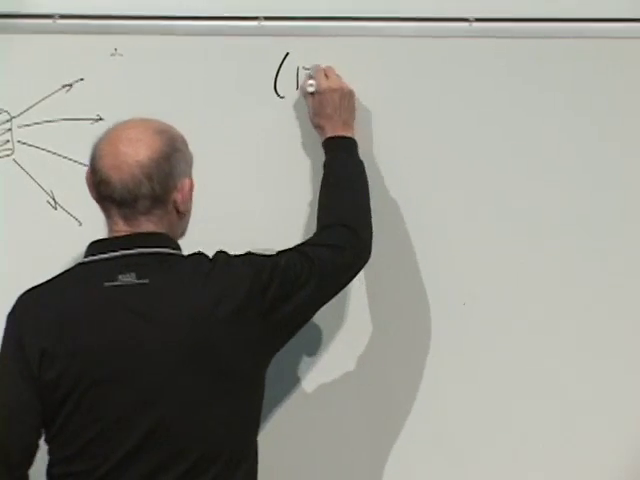
\includegraphics[width=0.66\textwidth]{lecture_06_figure_02.png}
  \caption{La condición de capa de masa en la convención métrica empleada a lo largo de la clase.}
  \lectureframe{00:05:56}
  \label{fig:l06-mass-shell}
\end{figure}

Consideremos dos partículas entrantes con momentos \(k_1,k_2\) y dos partículas salientes con momentos físicos \(q_3,q_4\). La conservación de la energía y el momento se expresa mediante una sola ecuación de cuatro vectores:
\begin{equation}
  k_1+k_2=q_3+q_4.
  \label{eq:l06-physical-conservation}
\end{equation}
Es conveniente asignar un momento entrante a cada línea externa:
\begin{equation}
  k_3\equiv-q_3,
  \qquad
  k_4\equiv-q_4.
\end{equation}
Entonces,
\begin{equation}
  k_1+k_2+k_3+k_4=0,
  \label{eq:l06-all-incoming}
\end{equation}
y cada pata satisface \(k_i^2=-m_i^2\). En esta convención contable, las partículas salientes tienen energía negativa; sus energías físicas siguen siendo positivas.

\begin{figure}[H]
  \centering
  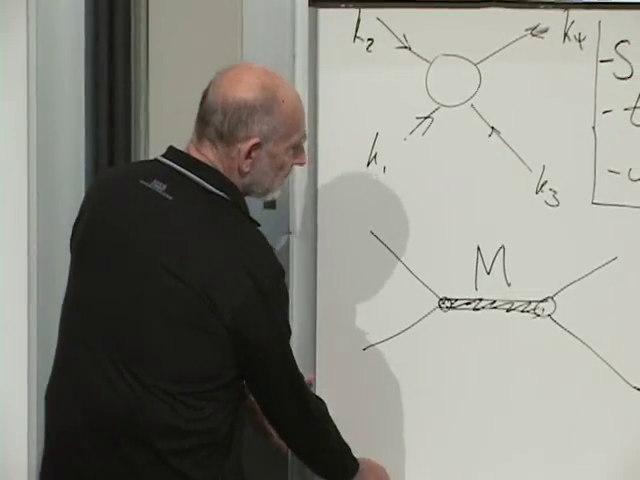
\includegraphics[width=0.68\textwidth]{lecture_06_figure_03.png}
  \caption{Se invierten los momentos físicos salientes para poder tratar simétricamente como entrantes los cuatro momentos externos.}
  \lectureframe{00:09:10}
  \label{fig:l06-all-incoming-board}
\end{figure}

Al principio, la amplitud parece ser una función de dieciséis componentes, \(\mathcal A(k_1,k_2,k_3,k_4)\). La mayoría son redundantes. Pasemos al sistema del centro de masas, orientemos los momentos entrantes a lo largo de un eje elegido y supongamos, para simplificar, que las cuatro partículas tienen la misma masa. El estado entrante queda entonces determinado por un solo número: la energía del centro de masas. Los momentos espaciales salientes deben ser iguales y opuestos, y tener el mismo módulo que los del par entrante. Solo queda el ángulo de desviación \(\theta\). Por tanto, el proceso tiene dos variables cinemáticas independientes:
\begin{equation}
  E_{\mathrm{cm}},
  \qquad
  \theta.
  \label{eq:l06-two-data}
\end{equation}

\section{Variables de Mandelstam}

Las dos cantidades físicas de \eqref{eq:l06-two-data} deberían poder expresarse sin elegir un sistema de referencia. Con la convención de todos entrantes, definamos
\begin{equation}
  \begin{aligned}
    -s&=(k_1+k_2)^2,\\
    -t&=(k_1+k_3)^2,\\
    -u&=(k_1+k_4)^2.
  \end{aligned}
  \label{eq:l06-mandelstam}
\end{equation}
En el sistema del centro de masas, las partes espaciales de \(k_1+k_2\) se cancelan; por tanto,
\begin{equation}
  s=E_{\mathrm{cm}}^2.
  \label{eq:l06-s-energy}
\end{equation}

Para un momento físico saliente \(q_3=-k_3\),
\begin{equation}
  k_1+k_3=k_1-q_3
\end{equation}
es el momento transferido de la pata 1 a la pata 3. Para masas externas iguales y un módulo del momento espacial entrante de \(p\),
\begin{equation}
  -t=2p^2(1-\cos\theta),
  \qquad
  -u=2p^2(1+\cos\theta).
  \label{eq:l06-tu-angle}
\end{equation}
Así, \(t\) y \(u\) contienen la información angular que miden los detectores.

\begin{figure}[H]
  \centering
  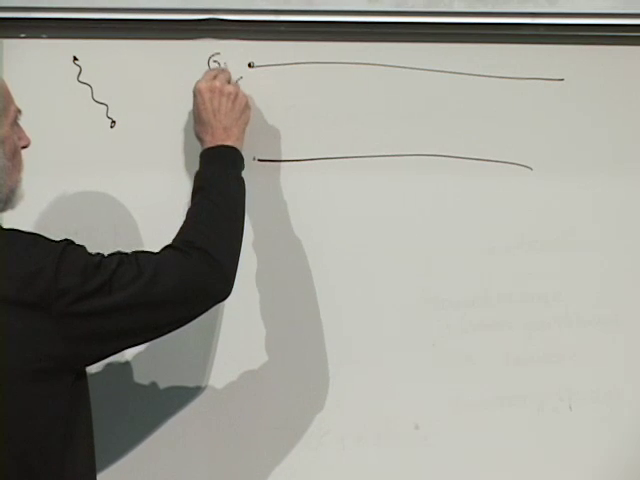
\includegraphics[width=0.74\textwidth]{lecture_06_figure_04.png}
  \caption{Las definiciones simétricas de \(s,t,u\) con la convención de todos entrantes.}
  \lectureframe{00:26:20}
  \label{fig:l06-stu-board}
\end{figure}

Que haya tres símbolos no significa que existan tres datos independientes. Al elevar al cuadrado \eqref{eq:l06-all-incoming} y usar \(k_i^2=-m^2\), se obtiene
\begin{equation}
  s+t+u=4m^2
  \label{eq:l06-stu-constraint}
\end{equation}
para masas iguales. Una vez conocidos \(s\) y \(t\), \(u\) queda determinado.

\begin{classroomqa}\audiencequestion{¿Podría el vacío frenar una partícula en movimiento libre, como si hubiera fricción? \lecturetimestamp{00:27:17}}\lecturerresponse{No en un vacío invariante bajo traslaciones. No hay dónde transferir el momento que falta, así que la conservación del momento prohíbe esa fricción. Se puede imaginar un medio u otro vacío que seleccione un sistema de reposo privilegiado, pero ese no es el vacío que consideramos aquí.}\end{classroomqa}

\begin{classroomqa}\audiencequestion{¿Por qué las dos partículas salientes deben tener la misma energía? \lecturetimestamp{00:27:54}}\lecturerresponse{En el sistema del centro de masas, sus momentos espaciales deben ser iguales y opuestos. En el proceso de masas iguales que estamos considerando, módulos de momento iguales implican energías iguales mediante \(E^2=p^2+m^2\). Si las masas de las partículas salientes fueran distintas, habría que modificar esa última conclusión.}\end{classroomqa}

\section{Canales directo y cruzado}

Un sencillo diagrama de partículas puntuales permite que las partículas 1 y 2 formen una partícula intermedia de masa \(M\), que luego se desintegra en 3 y 4. Salvo por factores en el numerador y la prescripción del polo, la dependencia característica es
\begin{equation}
  \mathcal A_s\sim\frac{g^2}{s-M^2}.
  \label{eq:l06-s-channel}
\end{equation}
Este es el proceso del canal directo, o canal \(s\). Si se gira la conectividad, se obtiene el intercambio entre las dos líneas externas:
\begin{equation}
  \mathcal A_t\sim\frac{g^2}{t-M^2},
  \label{eq:l06-t-channel}
\end{equation}
el proceso del canal cruzado, o canal \(t\). Una tercera conectividad da
\begin{equation}
  \mathcal A_u\sim\frac{g^2}{u-M^2}.
  \label{eq:l06-u-channel}
\end{equation}

\begin{figure}[H]
  \centering
  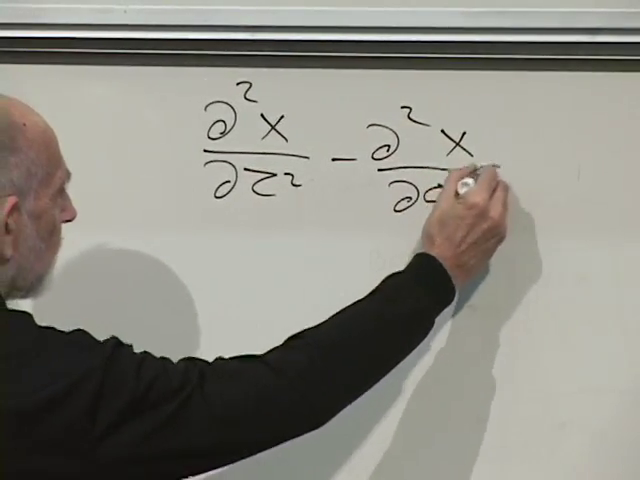
\includegraphics[width=0.72\textwidth]{lecture_06_figure_05.png}
  \caption{Producción directa mediante un estado intermedio y el polo correspondiente \(g^2/(s-M^2)\); la conectividad cruzada se está montando en el mismo tablero.}
  \lectureframe{00:30:50}
  \label{fig:l06-channel-board}
\end{figure}

La distinción es física. A este nivel escalar rudimentario, \eqref{eq:l06-s-channel} depende de la energía de colisión, pero no del ángulo. El estado compuesto ha perdido la dirección incidente antes de desintegrarse, por lo que su desintegración es isótropa. La amplitud de intercambio depende de la transferencia de momento y, por tanto, del ángulo; una partícula intercambiada ligera favorece mucho las desviaciones pequeñas. El espín añadiría más dependencia angular, pero la estructura de polos ya es visible.

\begin{classroomqa}\audiencequestion{¿El canal \(u\) que falta da lugar a un tercer término? \lecturetimestamp{00:34:47}}\lecturerresponse{Sí, siempre que las identidades de las partículas y sus acoplamientos permitan esa conectividad. En ese caso se incluye un término con un polo en \(u=M^2\). No es una nueva variable cinemática independiente, porque \(s+t+u=4m^2\), pero sí corresponde a un diagrama de canal distinto.}\end{classroomqa}

\section{Una función, dos descripciones de canal}

Un solo polo es un modelo pobre para la dispersión de mesones. Dos mesones pueden formar muchas resonancias, con una torre de masas y momentos angulares. La primera respuesta en la década de 1960 fue añadir más polos del canal \(s\), más polos del canal \(t\) y los polos permitidos del canal \(u\). Entonces se encontró una función mucho más económica. En las unidades de la clase, donde la trayectoria de Regge lineal y su intercepto se han absorbido en \(s\) y \(t\), la función es
\begin{equation}
  \mathcal A_{\mathrm V}(s,t)
  \propto
  \frac{\Gamma(-s)\Gamma(-t)}{\Gamma(-s-t)}.
  \label{eq:l06-veneziano}
\end{equation}
La función gamma extiende el factorial:
\begin{equation}
  \Gamma(n)=(n-1)!
\end{equation}
para enteros positivos.

\begin{figure}[H]
  \centering
  \includegraphics[width=0.68\textwidth]{lecture_06_figure_06.png}
  \caption{La amplitud de Veneziano escrita como un cociente simétrico de funciones gamma.}
  \lectureframe{00:42:25}
  \label{fig:l06-veneziano-board}
\end{figure}

Los polos de \(\Gamma(-s)\) reproducen una torre infinita de resonancias del canal directo. Sin embargo, la misma expresión es simétrica bajo \(s\leftrightarrow
t\), así que sus polos \(\Gamma(-t)\) dan una expansión del canal cruzado. No se trata de dos contribuciones añadidas por separado. Una sola función analítica admite ambas descripciones. Esta es la antigua idea de la dualidad entre las resonancias del canal directo y los intercambios del canal cruzado.

\begin{classroomqa}\audiencequestion{¿Cómo puede una amplitud contener las sumas de ambos canales sin sumarlas entre sí? \lecturetimestamp{00:43:32}}\lecturerresponse{Esa es precisamente la sorpresa. Al desarrollar la función cerca de sus polos del canal \(s\), se organiza como una serie de resonancias directas; al desarrollarla cerca de sus polos del canal \(t\), la misma función se organiza como una serie de intercambios. Hace falta un modelo microscópico que explique por qué ambas interpretaciones son la misma, y ese modelo es una cuerda interactuante.}\end{classroomqa}

\section{Una banda barrida por una cuerda abierta}

Parametricemos una cuerda abierta mediante
\begin{equation}
  0\leq\sigma\leq\pi.
\end{equation}
La etiqueta \(\sigma\) no es una posición en el espacio-tiempo. La inmersión \(X^\mu(\sigma,\tau)\) indica dónde se encuentra en el espacio-tiempo el punto que lleva esa etiqueta, mientras que \(\tau\) mide la evolución. Una partícula puntual barre una línea de mundo; una cuerda en movimiento barre una hoja de mundo bidimensional. En la teoría libre, cada coordenada de inmersión satisface
\begin{equation}
  \frac{\partial^2X^\mu}{\partial\tau^2}
  -
  \frac{\partial^2X^\mu}{\partial\sigma^2}
  =0.
  \label{eq:l06-wave-equation}
\end{equation}

\begin{figure}[H]
  \centering
  \includegraphics[width=0.70\textwidth]{lecture_06_figure_07.png}
  \caption{La ecuación de ondas que rige cada coordenada de la cuerda libre en la banda de la hoja de mundo.}
  \lectureframe{00:49:10}
  \label{fig:l06-wave-equation-board}
\end{figure}

Para construir la dispersión, conviene no tomar demasiado pronto el límite continuo. Sustituyamos cada cuerda por \(n\) masas puntuales unidas por resortes. La hoja de mundo se convierte en un conjunto denso de líneas de mundo próximas, y sus modos normales son osciladores armónicos ordinarios. Dos cadenas entrantes pueden tocarse por sus extremos. En ese instante se une un resorte nuevo, las cadenas evolucionan durante un tiempo \(\tau\) como una sola cadena más larga y, más adelante, se rompe un resorte para que emerjan dos cadenas salientes.

\begin{figure}[H]
  \centering
  \includegraphics[width=0.72\textwidth]{lecture_06_figure_08.png}
  \medskip

  \begin{tikzpicture}[x=0.85cm,y=0.70cm]
    \draw[thick] (0,2.2) -- (2.1,2.2) -- (3.1,1.5);
    \draw[thick] (0,0.8) -- (2.1,0.8) -- (3.1,1.5);
    \draw[thick] (3.1,1.5) -- (5.5,1.5);
    \draw[thick] (5.5,1.5) -- (6.5,2.2) -- (8.6,2.2);
    \draw[thick] (5.5,1.5) -- (6.5,0.8) -- (8.6,0.8);
    \draw[<->] (3.1,0.35) -- node[below] {\(\tau\)} (5.5,0.35);
    \node[left] at (0,2.2) {1};
    \node[left] at (0,0.8) {2};
    \node[right] at (8.6,2.2) {3};
    \node[right] at (8.6,0.8) {4};
  \end{tikzpicture}
  \caption{Dos cuerdas abiertas discretizadas se tocan, forman una sola cuerda intermedia durante un tiempo \(\tau\) y se separan. El fotograma de la fuente conserva la construcción con resortes y líneas de mundo; el esquema aísla la conectividad.}
  \lectureframe{00:51:25}
  \label{fig:l06-string-joining}
\end{figure}

Las dos cuerdas solo se dibujan juntas en el espacio de parámetros. No es necesario que sus posiciones en el espacio-tiempo estén próximas hasta que las coordenadas de sus extremos coincidan efectivamente. La libertad de reparametrización permite situar los eventos de unión y separación en posiciones convenientes del diagrama; en la próxima clase, esta libertad geométrica se convertirá en simetría conforme.

\section{El cálculo de osciladores paso a paso}

Sea la primera cadena la que tiene coordenadas \(x_1,\ldots,x_n\), y la segunda, la que tiene coordenadas \(x_{n+1},\ldots,x_{2n}\). Sus coordenadas del centro de masas son
\begin{equation}
  X_{\mathrm{cm}}^{(1)}
  =\frac1n\sum_{a=1}^{n}x_a,
  \qquad
  X_{\mathrm{cm}}^{(2)}
  =\frac1n\sum_{a=n+1}^{2n}x_a.
  \label{eq:l06-chain-centers}
\end{equation}
Una cadena con momento definido \(k_1\) tiene una onda plana para el centro de masas multiplicada por el estado fundamental de los osciladores internos:
\begin{align}
  \Psi_1
  &=
  e^{ik_1\cdot X_{\mathrm{cm}}^{(1)}}
  \psi_0(x_1,\ldots,x_n),
  \\
  \Psi_2
  &=
  e^{ik_2\cdot X_{\mathrm{cm}}^{(2)}}
  \psi_0(x_{n+1},\ldots,x_{2n}).
  \label{eq:l06-two-wavefunctions}
\end{align}
Los factores \(\psi_0\) dependen de las coordenadas relativas, no de la traslación conjunta de toda la cadena. Como las cuerdas entrantes son inicialmente sistemas cuánticos separados,
\begin{equation}
  \Psi_{\mathrm{in}}=\Psi_1\Psi_2.
  \label{eq:l06-product-state}
\end{equation}

\begin{figure}[H]
  \centering
  \includegraphics[width=0.76\textwidth]{lecture_06_figure_09.png}
  \caption{Las dos ondas planas de momento y sus factores de estado fundamental de los osciladores internos, representados en colores distintos.}
  \lectureframe{00:58:05}
  \label{fig:l06-wavefunctions-board}
\end{figure}

La unión selecciona la parte de esta función de onda en la que coinciden las coordenadas de los dos extremos:
\begin{equation}
  x_n=x_{n+1}.
  \label{eq:l06-endpoint-contact}
\end{equation}
En ese instante, las demás coordenadas no cambian. A continuación, el estado evoluciona con el hamiltoniano \(H_{\mathrm{joined}}\) de la única cadena más larga:
\begin{equation}
  \Psi(\tau)
  =
  e^{-iH_{\mathrm{joined}}\tau}\Psi(0).
  \label{eq:l06-time-evolution}
\end{equation}
Por último, se calcula su solapamiento con un producto de estados de cuerdas salientes con momentos \(q_3,q_4\).

\begin{figure}[H]
  \centering
  \includegraphics[width=0.76\textwidth]{lecture_06_figure_10.png}
  \caption{La función de onda de las dos cadenas justo antes de imponer la coincidencia de los extremos.}
  \lectureframe{00:58:55}
  \label{fig:l06-endpoint-board}
\end{figure}

El cálculo es largo, pero no encierra ningún misterio. Cada coordenada interna se puede descomponer en modos de oscilación, de modo que el solapamiento en la unión, la evolución temporal y la proyección final se reducen al álgebra gaussiana de osciladores. Lo que sigue sin determinarse es el tiempo de vida \(\tau\) de la cuerda unida.

\begin{classroomqa}\audiencequestion{¿Se suman o se multiplican las funciones de onda negra y roja? \lecturetimestamp{01:02:26}}\lecturerresponse{Se multiplican. En la representación de coordenadas, el estado producto tensorial de dos sistemas independientes viene dado por el producto de sus funciones de onda. La suma describiría una superposición de alternativas, no la presencia simultánea de las dos cuerdas entrantes.}\end{classroomqa}

\begin{classroomqa}\audiencequestion{¿Por qué se integra sobre el tiempo intermedio \(\tau\)? \lecturetimestamp{01:04:04}}\lecturerresponse{No se asigna un tiempo de vida fijo a la cuerda unida. La regla de Feynman consiste en sumar las amplitudes de todas las historias posibles. En esta descripción, el parámetro continuo de historia que queda es el tiempo transcurrido entre la unión y la separación, así que la suma se convierte en una integral sobre \(0\leq\tau<\infty\).}\end{classroomqa}

\section{Del tiempo de propagación a la función beta}

Tras evaluar los solapamientos de los osciladores, el resultado puede escribirse como
\begin{equation}
  \mathcal A(s,t)
  \propto
  \int_0^\infty d\tau\,
  e^{\tau(s+1)}
  \bigl(1-e^{-\tau}\bigr)^{-t-1}
  e^{-\tau}.
  \label{eq:l06-tau-integral}
\end{equation}
Se mantiene explícito el factor final \(e^{-\tau}\) porque es el jacobiano necesario en el siguiente paso. De manera equivalente, las exponenciales primera y última se combinan para dar \(e^{s\tau}\).

\begin{figure}[H]
  \centering
  \includegraphics[width=0.76\textwidth]{lecture_06_figure_11.png}
  \caption{El integrando respecto al tiempo de propagación tras el cálculo de los osciladores; el factor \(e^{-\tau}\) separado proporciona el jacobiano del cambio de variable.}
  \lectureframe{01:06:45}
  \label{fig:l06-tau-integral-board}
\end{figure}

Hagamos ahora el cambio
\begin{equation}
  z=e^{-\tau},
  \qquad
  dz=-e^{-\tau}\,d\tau.
  \label{eq:l06-z-substitution}
\end{equation}
Cuando \(\tau\) varía de \(0\) a \(\infty\), \(z\) varía de \(1\) a \(0\). El signo menos invierte los límites y se obtiene
\begin{equation}
  \mathcal A(s,t)
  \propto
  \int_0^1
  z^{-s-1}(1-z)^{-t-1}\,dz.
  \label{eq:l06-beta-integral}
\end{equation}

\begin{figure}[H]
  \centering
  \includegraphics[width=0.74\textwidth]{lecture_06_figure_12.png}
  \caption{El cambio de variable \(z=e^{-\tau}\) hace aparecer la integral beta de Euler.}
  \lectureframe{01:08:49}
  \label{fig:l06-beta-integral-board}
\end{figure}

Esta integral se define directamente en la región donde converge en sus extremos y, fuera de ella, mediante continuación analítica. Es la función beta de Euler:
\begin{equation}
  B(-s,-t)
  =
  \frac{\Gamma(-s)\Gamma(-t)}{\Gamma(-s-t)}.
  \label{eq:l06-beta-gamma}
\end{equation}

\begin{figure}[H]
  \centering
  \includegraphics[width=0.72\textwidth]{lecture_06_figure_13.png}
  \caption{El tablero identifica la integral transformada con \(B(-s,-t)\) y empieza a recuperar su expresión en términos de funciones gamma.}
  \lectureframe{01:12:24}
  \label{fig:l06-beta-gamma-board}
\end{figure}

La simetría entre canales resulta ahora inmediata. Bajo \(z\mapsto1-z\),
\begin{equation}
  \int_0^1 z^{-s-1}(1-z)^{-t-1}\,dz
  =
  \int_0^1 z^{-t-1}(1-z)^{-s-1}\,dz.
\end{equation}
Por tanto, \(\mathcal A(s,t)=\mathcal A(t,s)\). Un proceso construido a partir de dos cuerdas que se unen y luego se separan contiene automáticamente también la descripción cruzada.
\editorialnote{En los argumentos de la función beta, la clase omite la pendiente y el intercepto de Regge. En notación estándar, se sustituye \(s,t\) por las trayectorias lineales correspondientes \(\alpha(s),\alpha(t)\). La dualidad y el argumento basado en el cambio de variable no cambian.}

\begin{classroomqa}\audiencequestion{El cociente de funciones gamma se parece a expresiones con factoriales de combinatoria. ¿Tiene una interpretación directa como conteo físico? \lecturetimestamp{01:13:22}}\lecturerresponse{Para argumentos enteros, la función beta está relacionada con un cociente como \(n!\,m!/(n+m)!\), pero aquí no se propone ningún mecanismo combinatorio. La misma función especial aparece en la integral sobre la hoja de mundo; esta semejanza no fue el camino por el que se encontró la amplitud.}\end{classroomqa}

La razón, todavía oculta, por la que una misma hoja de mundo admite ambas interpretaciones de canal es la simetría conforme. Esta permite estirar la hoja como si fuera una masa elástica sin cambiar la amplitud, convirtiendo una región de propagación larga del canal directo en una imagen de intercambio del canal cruzado. La explicación geométrica queda para la próxima clase.

\section{Qué estableció la prueba de dispersión}
\enlargethispage{3\baselineskip}
\begingroup
\setlength{\medskipamount}{3pt plus 1pt minus 1pt}

La imagen discreta de la unión dio pie a un último grupo de preguntas.

\begin{classroomqa}\audiencequestion{Si se unen por los extremos dos cadenas de \(n\) constituyentes, ¿el resultado tiene \(2n-1\), y podría eso cambiar la paridad fermiónica? \lecturetimestamp{01:16:16}}\lecturerresponse{En la imagen hadrónica de los extremos, el par de extremos que se toca puede interpretarse como un par partícula-antipartícula que se aniquila, por lo que el número se reduce en dos, no en uno. En el límite continuo, la diferencia finita entre \(2n\) y \(2n-2\) no importa, pero conservar la paridad fermiónica sí importa. Los constituyentes de la red solo sirven como regulador de la cuerda continua; no son bolitas fundamentales literales.}\end{classroomqa}

\begin{classroomqa}\audiencequestion{¿La discusión posterior abordará toda la matemática de las supercuerdas? \lecturetimestamp{01:18:05}}\lecturerresponse{Solo se usarán algunas consecuencias. El camino inmediato pasa por la simetría de la hoja de mundo y la compactificación, y luego parte de un enfoque distinto desarrollado a mediados de la década de 1990: la teoría M. Su propósito es llegar a la misma física desde un punto de vista que vuelve transparentes varias características que, de otro modo, son complicadas.}\end{classroomqa}

\begin{classroomqa}\audiencequestion{¿Esta regla de unión era solo una pista obtenida de las colisiones de mesones? \lecturetimestamp{01:20:02}}\lecturerresponse{La dispersión de mesones proporcionó la pista histórica, pero la regla es general para las cuerdas abiertas. La misma topología describe las colisiones de fotones de cuerda abierta y de otros estados de cuerda abierta. Dos cuerdas cerradas se unen y se separan mediante una construcción análoga, con una cuerda cerrada en la región intermedia.}\end{classroomqa}

\begin{classroomqa}\audiencequestion{¿El cálculo se aplica solo cuando los estados de cuerda son fermiones? \lecturetimestamp{01:20:56}}\lecturerresponse{No. El cálculo original de Veneziano corresponde a la cuerda abierta bosónica. Las supercuerdas requieren grados de libertad fermiónicos adicionales y modifican detalles del integrando, pero la lógica de unión, propagación, proyección y dualidad de la hoja de mundo sigue siendo muy similar.}\end{classroomqa}

Encontrar un estado de espín uno o espín dos en el espectro de osciladores era sugerente, pero no concluyente. Las amplitudes de dispersión de esos estados proporcionaron una prueba más sólida. Las amplitudes de fotones satisfacen las identidades asociadas a la conservación de la carga y la invariancia gauge; las de gravitones satisfacen las restricciones correspondientes a un campo sin masa de espín dos. Los estados de cuerda superaron estas pruebas en interacciones con estados masivos y sin masa, así como entre sí. Por eso, las denominaciones de fotón y gravitón pasaron a ser identificaciones físicas, en lugar de conjeturas basadas solo en contar polarizaciones.
\editorialnote{En lenguaje moderno, estas pruebas se expresan mediante la desacoplación de las polarizaciones no físicas, las identidades de Ward gauge y el acoplamiento universal de baja energía del estado sin masa de espín dos.}

\begin{classroomqa}\audiencequestion{¿De dónde proviene la propia carga eléctrica en la descripción de cuerdas? \lecturetimestamp{01:24:03}}\lecturerresponse{La clase termina dejando abierta esa pregunta. Su respuesta requiere la estructura interna y la estructura de los extremos de la teoría de cuerdas, que todavía no se han presentado; por eso corresponde a la discusión que sigue, no a esta derivación de la dispersión.}\end{classroomqa}
\endgroup

\chapter{Hojas de universo, rotación de Wick y dualidad entre canales}

\lectureoverview{Una partícula recorre una línea de universo; una cuerda barre una hoja de universo. Cuantizar cualquiera de estos objetos requiere sumar sobre las historias posibles, pero la suma lorentziana es oscilatoria y difícil de definir. Al convertir el tiempo de la hoja de universo en una coordenada imaginaria, se obtiene una teoría euclídea regida por la ecuación de Laplace. Su simetría conforme permite entonces transformar la superficie con cortes de una interacción entre cuatro cuerdas en un disco con cuatro inserciones en el borde, donde se hace visible la simetría entre los canales directo y cruzado.}

\section{De la línea de universo a la suma sobre historias}

Empecemos con una partícula libre. En mecánica no relativista, su posición es una función \(\mathbf x(t)\) y, tomando la masa igual a uno, su acción es \begin{equation}
  S_{\mathrm{NR}}[\mathbf x]
  =\frac12\int_{t_1}^{t_2}\dot{\mathbf x}^{\,2}\,dt.
  \label{eq:l07-nr-action}
\end{equation} Para una descripción relativista, resulta más natural reunir el tiempo y el espacio en un vector, \(X^\mu(\tau)\), parametrizado a lo largo de la trayectoria mediante \(\tau\). La expresión cuadrática correspondiente es \begin{equation}
  S_{\mathrm{rel}}[X]
  =\frac12\int_{\tau_1}^{\tau_2}
  \frac{dX^\mu}{d\tau}\frac{dX_\mu}{d\tau}\,d\tau.
  \label{eq:l07-rel-action}
\end{equation} Los índices superiores e inferiores codifican la diferencia de signo lorentziana entre el tiempo y el espacio. \editorialnote{La acción relativista cuadrática se utiliza con una parametrización fija de la línea de universo. La alternativa manifiestamente invariante bajo reparametrizaciones es proporcional a la longitud propia, que se menciona más adelante en la conferencia.}

\begin{figure}[H]\centering
  \includegraphics[width=0.72\textwidth]{lecture_07_figure_01.png}\caption{Las acciones no relativista y relativista cuadrática, escritas juntas en la pizarra.}\lectureframe{00:03:35}\label{fig:l07-particle-actions}\end{figure}

Clásicamente, se fijan los extremos y se varía la trayectoria. La partícula libre sigue entonces una línea de universo recta con velocidad constante. La mecánica cuántica plantea otra pregunta. No selecciona una única trayectoria entre los extremos; pregunta cuál es la amplitud de que la partícula comience en un punto y se detecte en el otro. Cada trayectoria intermedia contribuye con una fase, \begin{equation}
  K(2,1)=\int_{X(1)}^{X(2)}\!\mathcal D X\,
  e^{iS[X]}.
  \label{eq:l07-feynman-integral}
\end{equation} La integral funcional es una integral sobre un espacio infinito-dimensional de trayectorias, no la integral ordinaria que ya aparece dentro de la acción.

\begin{figure}[H]\centering
  \includegraphics[width=0.72\textwidth]{lecture_07_figure_02.png}\caption{Una trayectoria representativa y la fase que se le asigna antes de efectuar la suma sobre todas las trayectorias.}\lectureframe{00:06:21}\label{fig:l07-path-integral-board}\end{figure}

En lenguaje relativista, esta amplitud entre dos puntos es un propagador. En una interacción, se unen varios segmentos de líneas de universo. Se suman sus acciones, se integra sobre los puntos de unión y se suman los diagramas con las partículas externas requeridas. Así pues, la conocida expansión en diagramas de Feynman ya está implícita en la instrucción de sumar sobre las historias.

Aquí, el símbolo \(S\) denotará una acción. No guarda relación ni con la entropía ni con la variable de Mandelstam \(s\) que se usa cerca del final de la conferencia. La notación compartida es tradicional, pero poco esclarecedora.

\section{Girar el tiempo hacia una dirección imaginaria}

Hay un problema inmediato con \eqref{eq:l07-feynman-integral}. Cada factor \(e^{iS}\) tiene módulo uno. Por tanto, una trayectoria que se aleja mucho y oscila intensamente y la línea recta clásica entran con el mismo peso absoluto; solo difieren sus fases. La interferencia destructiva recupera el comportamiento clásico, pero no convierte la integral formal en un objeto ordinario convergente.

Introduzcamos un nuevo parámetro \(s\) mediante \begin{equation}
  \tau=\alpha s,
  \qquad
  d\tau=\alpha\,ds,
  \qquad
  \frac{dX}{d\tau}=\frac{1}{\alpha}\frac{dX}{ds}.
\end{equation} Entonces, la acción cuadrática se reescala así: \begin{equation}
  \frac12\int d\tau
  \left(\frac{dX}{d\tau}\right)^2
  =
  \frac{1}{2\alpha}\int ds
  \left(\frac{dX}{ds}\right)^2.
  \label{eq:l07-rescaled-action}
\end{equation} Elegir el contorno correspondiente a \(\alpha=-i\) transforma el peso oscilatorio en \begin{equation}
  e^{iS}
  \longrightarrow
  \exp\!\left[-\frac12\int ds
  \left(\frac{dX}{ds}\right)^2\right]
  =e^{-S_E}.
  \label{eq:l07-euclidean-particle}
\end{equation}

\begin{figure}[H]\centering
  \includegraphics[width=0.66\textwidth]{lecture_07_figure_03.png}\caption{El peso euclídeo de la partícula tras la sustitución de tiempo imaginario; el exponente es real y no positivo.}\lectureframe{00:16:20}\label{fig:l07-particle-wick}\end{figure}

Una trayectoria que se aleja mucho y regresa, o que oscila rápidamente sin recorrer una gran distancia, tiene un valor grande y positivo de \(S_E\) y queda suprimida exponencialmente. El resultado es una integral de tipo Wiener, para la cual existe una teoría de la convergencia rigurosa. Los extremos heredados de valores reales de \(\tau\) se encuentran sobre un contorno imaginario de \(s\). En la práctica, se evalúa el objeto euclídeo en su dominio de convergencia y después se continúa analíticamente la respuesta hasta recuperar las variables lorentzianas físicas. Esta operación es la rotación de Wick: para el cálculo se ha girado el tiempo hacia una dirección imaginaria, no se lo ha descartado.

\section{De las líneas de universo a las hojas de universo}

Una partícula puntual tiene una línea de universo. Una cuerda abierta barre una cinta, y una cuerda cerrada barre un tubo. Las coordenadas \((\sigma,\tau)\) señalan puntos de esta hoja de universo bidimensional, mientras que \begin{equation}
  X^\mu=X^\mu(\sigma,\tau)
  \label{eq:l07-embedding}
\end{equation} da la posición en el espacio-tiempo del punto señalado. Conocer todas las funciones \(X^\mu\) especifica la historia completa de la cuerda.

La acción cuadrática lorentziana de la hoja de universo tiene la misma estructura de energía cinética menos energía potencial que la de una cuerda vibrante ordinaria: \begin{equation}
  S_{\mathrm{ws}}[X]
  =\frac{T_s}{2}\int d\tau\,d\sigma\,
  \left[
    \partial_\tau X^\mu\partial_\tau X_\mu
    -
    \partial_\sigma X^\mu\partial_\sigma X_\mu
  \right].
  \label{eq:l07-lorentzian-worldsheet}
\end{equation} La tensión total \(T_s\) fija la escala; en esta conferencia se omite mientras se presta atención a la estructura de las derivadas.

\begin{figure}[H]\centering
  \includegraphics[width=0.72\textwidth]{lecture_07_figure_04.png}\caption{La acción lorentziana de la hoja de universo para \(X^\mu(\sigma,\tau)\), con el signo de energía cinética menos energía potencial.}\lectureframe{00:24:26}\label{fig:l07-worldsheet-action}\end{figure}

La amplitud de la cuerda se obtiene exponenciando esta acción y sumando sobre todas las superficies que conectan las configuraciones iniciales y finales prescritas de la cuerda: \begin{equation}
  \mathcal A=\int\mathcal D X\,e^{iS_{\mathrm{ws}}[X]}.
  \label{eq:l07-surface-integral}
\end{equation} La misma regla describe dos cuerdas que se convierten en dos, en tres o en cualquier otra configuración externa permitida. La suma incluye también distintas topologías de la hoja de universo. Añadir agujeros es el equivalente, en teoría de cuerdas, a añadir órdenes de bucle en una expansión de diagramas de partículas puntuales.

\begin{figure}[H]\centering
  \includegraphics[width=0.66\textwidth]{lecture_07_figure_05.png}\caption{Una superficie que conecta varias cuerdas externas, con un agujero que representa otra topología de la hoja de universo.}\lectureframe{00:27:14}\label{fig:l07-surface-topology}\end{figure}

\begin{classroomqa}\audiencequestion{Para un electrón puntual, ¿se anula simplemente la derivada respecto de \(\sigma\)? \lecturetimestamp{00:27:56}}\lecturerresponse{Una partícula puntual ni siquiera tiene coordenada \(\sigma\). Aun así, los dibujos están relacionados: cuando los estados externos son ligeros en comparación con la escala de cuerdas y las energías del proceso son bajas, las amplitudes de cuerdas reproducen los diagramas de Feynman ordinarios de partículas puntuales. Ese límite va mucho más allá de hacer que una derivada se anule.}\end{classroomqa}

La integral sobre superficies tiene el mismo problema de convergencia que la integral sobre trayectorias. Tras aplicar la rotación de Wick al tiempo de la hoja de universo, su forma euclídea estable es \begin{equation}
  \begin{aligned}
    S_{E,\mathrm{ws}}[X]
    &=\frac{T_s}{2}\int d\tau\,d\sigma\,
      \left[
        \partial_\tau X^\mu\partial_\tau X_\mu
        +\partial_\sigma X^\mu\partial_\sigma X_\mu
      \right],\\
    \mathcal A_E&=\int\mathcal D X\,e^{-S_{E,\mathrm{ws}}}.
  \end{aligned}
  \label{eq:l07-euclidean-worldsheet}
\end{equation} Ahora ambas derivadas aparecen con el mismo signo positivo. Una superficie que vibra violentamente o está muy estirada tiene una acción euclídea grande y queda suprimida.

\begin{figure}[H]\centering
  \includegraphics[width=0.72\textwidth]{lecture_07_figure_06.png}\caption{La densidad euclídea positiva de la hoja de universo después de rotar \(\tau\) a tiempo imaginario.}\lectureframe{00:34:29}\label{fig:l07-worldsheet-wick}\end{figure}

También existe una formulación geométricamente directa. A una partícula relativista se le puede asignar una acción proporcional a la longitud propia de su trayectoria; a una cuerda, una acción proporcional al área de su hoja de universo en el espacio-tiempo. Esta última es la acción de Nambu--Goto. La forma cuadrática de la hoja de universo que se usa aquí se denomina convencionalmente forma de Polyakov y resulta mucho más sencilla para el cálculo presente. \editorialnote{La conferencia incluye una discusión humorística sobre la atribución histórica de los nombres y menciona también la acción de Liouville, relacionada con ella, y las condiciones de contorno de Dirichlet. Para la derivación no hace falta reivindicar ninguna prioridad: solo se usa la equivalencia entre las formulaciones mediante el área y la métrica auxiliar.}

\section{La ecuación euclídea del movimiento}

Las coordenadas \(\sigma\) y \(\tau\) son solo etiquetas sobre la hoja. Así que la siguiente pregunta es inevitable: ¿qué cambios de etiquetas dejan invariante la teoría? La respuesta se ve más fácilmente a partir de la ecuación del movimiento. Al variar \eqref{eq:l07-euclidean-worldsheet} se obtiene, componente a componente, \begin{equation}
  \partial_\tau^2X^\mu+\partial_\sigma^2X^\mu=0.
  \label{eq:l07-laplace}
\end{equation} Antes de la rotación de Wick, el signo relativo es negativo y se trata de una ecuación de ondas. En signatura euclídea, ambos signos son positivos, por lo que se trata de la ecuación de Laplace bidimensional.

\begin{classroomqa}\audiencequestion{¿Es esta la ecuación de un tambor vibrante?\lecturetimestamp{00:41:50}}\lecturerresponse{Está estrechamente relacionada, pero un tambor vibrante también tiene una coordenada de tiempo real y, por tanto, obedece una ecuación de ondas. La ecuación de aquí es la ecuación de Laplace euclídea. El potencial electrostático en una región sin cargas es un ejemplo familiar más directo.}\end{classroomqa}

\begin{classroomqa}\audiencequestion{La acción contiene primeras derivadas. ¿Por qué su ecuación contiene segundas derivadas? \lecturetimestamp{00:42:44}}\lecturerresponse{Al variar un término cuadrático en una primera derivada e integrar por partes, una derivada pasa a actuar sobre esa primera derivada. Es la versión para campos de que \(\dot x^{\,2}\) en una acción produce \(\ddot x\) en la ecuación del movimiento.}\end{classroomqa}

\begin{figure}[H]\centering
  \includegraphics[width=0.68\textwidth]{lecture_07_figure_07.png}\caption{La ecuación de Laplace con signos positivos y la primera línea discreta que se usa para interpretar sus segundas derivadas.}\lectureframe{00:43:30}\label{fig:l07-laplace-board}\end{figure}

Para visualizar la geometría, discreticemos primero una coordenada con separación \(\epsilon\). Una primera derivada es una diferencia entre puntos vecinos, mientras que una segunda derivada es una diferencia entre diferencias de puntos vecinos: \begin{equation}
  \frac{d^2X}{ds^2}\bigg|_{2}
  \longrightarrow
  \frac{X(3)-2X(2)+X(1)}{\epsilon^2}.
  \label{eq:l07-second-difference}
\end{equation}

\begin{figure}[H]\centering
  \includegraphics[width=0.72\textwidth]{lecture_07_figure_08.png}\caption{La línea numerada, un pequeño fragmento de retícula y el desarrollo en diferencias finitas de una segunda derivada.}\lectureframe{00:45:51}\label{fig:l07-finite-difference-board}\end{figure}

Ahora discreticemos el plano \((\sigma,\tau)\). Denotemos por \(1,2,3,4\) los cuatro vecinos más próximos de un punto central \(5\). La ecuación \eqref{eq:l07-laplace} se convierte en \begin{equation}
  X(1)+X(2)+X(3)+X(4)-4X(5)=0,
\end{equation} o bien \begin{equation}
  X(5)=\frac14\bigl[X(1)+X(2)+X(3)+X(4)\bigr].
  \label{eq:l07-mean-value}
\end{equation}

\begin{figure}[H]\centering
  \includegraphics[width=0.72\textwidth]{lecture_07_figure_09.png}\caption{La ecuación bidimensional completa en diferencias finitas: el valor central es igual al promedio de sus cuatro vecinos.}\lectureframe{00:48:26}\label{fig:l07-mean-value-board}\end{figure}

Esta propiedad del valor medio se cumple para un cuadrado infinitesimal con cualquier orientación. Es el contenido geométrico local de la ecuación de Laplace y el vínculo con la simetría conforme.

\section{Coordenadas conformes}

Consideremos un cambio de \((\sigma,\tau)\) a \((\sigma',\tau')\). Una deformación general transforma un cuadrado pequeño en un cuadrilátero cualquiera. Las transformaciones especiales que nos interesan aquí llevan cada cuadrado infinitesimal a otro cuadrado infinitesimal, quizá rotado y reescalado. De manera equivalente, conservan los ángulos con que se cortan las curvas. Son las transformaciones conformes.

\begin{figure}[H]\centering
  \includegraphics[width=0.68\textwidth]{lecture_07_figure_10.png}\caption{Un cuadrado local se transforma en otra figura pequeña; se comprueba si se conservan sus ángulos.}\lectureframe{00:53:25}\label{fig:l07-conformal-board}\end{figure}

\begin{classroomqa}\audiencequestion{Si se conservan los ángulos, ¿la transformación consiste básicamente solo en una rotación? \lecturetimestamp{00:53:31}}\lecturerresponse{Solo localmente, e incluso en ese caso se permite también un cambio común de escala. La rotación local y el factor de escala pueden variar de un punto a otro, de modo que la cuadrícula de coordenadas puede curvarse, expandirse en una región y contraerse en otra, conservando las formas infinitesimales.}\end{classroomqa}

Una aplicación que conserva los ángulos no tiene por qué conservar el tamaño. Si también se conservara el tamaño en todas partes, las posibilidades se reducirían a la clase mucho más restringida de movimientos rígidos: traslaciones y rotaciones. En cambio, las aplicaciones conformes conservan la forma local. Por eso una proyección cartográfica puede preservar la forma de una isla pequeña y, aun así, distorsionar mucho su área.

\begin{classroomqa}\audiencequestion{¿Decir que una aplicación es conforme equivale a decir que el sistema de coordenadas es plano? \lecturetimestamp{00:55:35}}\lecturerresponse{No. La planitud y la conformidad son propiedades distintas. Una aplicación conforme puede utilizar líneas de coordenadas curvas; lo que conserva es el ángulo entre curvas que se cortan. Una proyección cartográfica de tipo Mercator es un ejemplo conocido que preserva la forma local con una distorsión considerable de la escala.}\end{classroomqa}

En dos dimensiones, las transformaciones requeridas se generan localmente mediante funciones analíticas de una coordenada compleja \begin{equation}
  z=\sigma+i\tau.
\end{equation} Los bordes finitos pueden cambiar de aspecto de manera drástica. Una región cuadrada puede transformarse en una región lisa, de modo que las esquinas originales se envíen a puntos ordinarios del nuevo borde y no a sus puntos más destacados visualmente. No hay contradicción: la conformidad es una condición local en el interior, y la aplicación conserva los ángulos infinitesimales allí donde es regular.

\begin{classroomqa}\audiencequestion{¿Es esta libertad de coordenadas la razón por la que se podía elegir de forma simétrica el diagrama anterior de unión--separación?\lecturetimestamp{00:56:32}}\lecturerresponse{Sí. La misma libertad conforme que conserva las ecuaciones de la hoja de universo nos permite reemplazar la incómoda franja de interacción por un dominio más simétrico. La libertad restante no elimina el parámetro físico de unión--separación; lo representa de nuevo como la posición relativa de las inserciones en el borde.}\end{classroomqa}

\section{La hoja con cortes y el disco}

Volvamos a la dispersión de cuatro cuerdas. Entran dos cuerdas abiertas, se unen sus extremos, la cuerda resultante se propaga y, más tarde, se divide. Dibujado como una hoja de universo plana, el proceso es una franja infinita con un corte en cada extremo. La separación \(\tau_0\) entre las puntas de los cortes es el tiempo de vida de la cuerda intermedia, y la amplitud se integra sobre ese parámetro.

\begin{figure}[H]\centering
  \includegraphics[width=0.72\textwidth]{lecture_07_figure_11.png}\caption{La franja con dos cortes representa dos cuerdas abiertas que se unen, se propagan juntas y vuelven a separarse.}\lectureframe{01:00:20}\label{fig:l07-slit-strip}\end{figure}

Tras la euclidianización, los campos de inmersión en esta región satisfacen la ecuación de Laplace. Por tanto, la invariancia conforme permite transformar la franja con cortes en un disco. Para visualizar la topología, se puede foliar el disco con círculos concéntricos y deformar continuamente esas curvas cerradas hasta que recubran la región con cortes. Bajo esta aplicación, los extremos en el infinito se convierten en puntos excepcionales del borde.

\begin{figure}[H]
  \centering
  \includegraphics[width=0.72\textwidth]{lecture_07_figure_12.png}
  \medskip

\begin{adjustbox}{max width=\linewidth}\begin{tikzpicture}[x=0.75cm,y=0.75cm]
    \draw[thick] (-5,1.2) -- (-1.2,1.2) -- (-0.35,0.35);
    \draw[thick] (-5,-1.2) -- (-1.2,-1.2) -- (-0.35,-0.35);
    \draw[thick] (0.35,0.35) -- (1.2,1.2) -- (5,1.2);
    \draw[thick] (0.35,-0.35) -- (1.2,-1.2) -- (5,-1.2);
    \draw[->,thick] (5.6,0) -- (7.0,0);
    \draw[thick] (9.0,0) circle (1.45);
    \foreach \a in {40,140,220,320} \fill (9.0,0) ++(\a:1.45) circle (1.5pt);
    \node[below] at (0,-1.65) {slit strip};
    \node[below] at (9.0,-1.65) {disc};
  \end{tikzpicture}\end{adjustbox}\caption{Comparación de las curvas de nivel de la pizarra y esquema limpio de la aplicación conforme de la franja con cortes a un disco. Los cuatro extremos externos se convierten en cuatro puntos especiales del borde.}\lectureframe{01:04:46}\label{fig:l07-strip-to-disc}\end{figure}

Los estados externos no se pierden en este cambio de coordenadas. En los cuatro puntos excepcionales hay que insertar el momento, el tipo de partícula y el nivel de oscilador. Los objetos formales que transportan esa información son los operadores vértice. Su construcción detallada se deja para más adelante, pero su función ya está clara: convierten una integral de caminos sobre la hoja de universo, por lo demás homogénea, en un experimento de dispersión especificado.

Tras usar transformaciones conformes del disco para llevar tres puntos del borde a posiciones de referencia convenientes, queda una posición relativa real. Se puede representar mediante la razón doble de los cuatro puntos ordenados del borde. Esta es la versión en el disco del antiguo tiempo de vida \(\tau_0\).

\begin{figure}[H]\centering
  \includegraphics[width=0.62\textwidth]{lecture_07_figure_13.png}\caption{Cuatro puntos de inserción en el borde del disco. La libertad conforme elimina todos los grados de libertad salvo un módulo real de su configuración ordenada.}\lectureframe{01:10:55}\label{fig:l07-four-points}\end{figure}

Por tanto, la integral sobre el tiempo de vida no ha desaparecido. Se ha convertido en una integral sobre el módulo restante. Con la coordenada convencional \(0<z<1\), la integral de cuatro puntos de cuerda abierta adopta la misma forma que en la conferencia anterior: \begin{equation}
  \mathcal A(s,t)\propto
  \int_0^1 z^{-s-1}(1-z)^{-t-1}\,dz.
  \label{eq:l07-modulus-integral}
\end{equation}

\section{Dos límites de una misma superficie}

En un extremo del espacio de módulos, los dos puntos de inserción asociados al par entrante se acercan entre sí. En las coordenadas de la franja con cortes, esto corresponde a un intervalo largo entre la unión y la separación: una cuerda intermedia del canal directo se propaga durante mucho tiempo. En el otro extremo, se acerca otro par de puntos vecinos. Entonces, la misma superficie se interpreta de manera natural como un intercambio en el canal cruzado. En la franja, estas descripciones parecen no tener relación, pero son límites vecinos de borde de una misma integral sobre el disco.

Volviendo a la convención de signatura mayoritariamente positiva de la conferencia anterior, \begin{equation}
  -s=(k_1+k_2)^2,
  \qquad
  -t=(k_1+k_3)^2.
  \label{eq:l07-mandelstam}
\end{equation} El límite directo organiza los polos en \(s\); el límite cruzado organiza los polos en \(t\). \editorialnote{Cerca del final de la conferencia, la pizarra usa un signo abreviado para los invariantes de Mandelstam y, al mismo tiempo, identifica \(s\) con la energía positiva del centro de masas al cuadrado. La ecuación \eqref{eq:l07-mandelstam} mantiene la convención de signatura mayoritariamente positiva establecida en la conferencia 6.}

\begin{figure}[H]\centering
  \includegraphics[width=0.62\textwidth]{lecture_07_figure_14.png}\caption{Los diagramas de los dos canales: propagación prolongada en una orientación e intercambio en la orientación cruzada.}\lectureframe{01:19:27}\label{fig:l07-channel-diagrams}\end{figure}

\begin{figure}[H]\centering
  \includegraphics[width=0.72\textwidth]{lecture_07_figure_15.png}\caption{La pizarra vuelve a las asignaciones de momentos de los canales \(s\) y \(t\) al comparar los dos límites del módulo del disco.}\lectureframe{01:19:40}\label{fig:l07-st-board}\end{figure}

Por tanto, un mismo objeto analítico proporciona ambas expansiones: \begin{equation}
  \mathcal A(s,t)=\mathcal A(t,s).
\end{equation} Esto es la dualidad entre canales. En el lenguaje original de las resonancias, resultaba milagroso que una suma sobre estados del canal directo pudiera codificar también el intercambio en el canal cruzado. En la hoja de universo euclídea, la simetría conforme explica por qué ambas descripciones corresponden a una misma superficie. Históricamente, esta interpretación llegó muy poco después del descubrimiento, en 1969, de la amplitud de Veneziano.

\begin{classroomqa}\audiencequestion{¿Existe también una representación de la franja con cortes para la orientación cruzada? \lecturetimestamp{01:20:49}}\lecturerresponse{Sí, pero hay que elegir de otra manera la dirección que se llama tiempo. La misma superficie euclídea se puede cortar de modo que otro par de extremos externos quede en el pasado y el futuro remotos. Precisamente ese corte alternativo permite que una misma hoja de universo admita más de una interpretación por canales.}\end{classroomqa}

\begin{classroomqa}\audiencequestion{¿El tiempo durante el que las cuerdas permanecen unidas está determinado por la constante de acoplamiento? \lecturetimestamp{01:21:39}}\lecturerresponse{No se selecciona un tiempo de vida fijo. El tiempo de vida es una variable de integración y contribuyen todos sus valores. La constante de acoplamiento controla el peso de la unión y la separación---, es decir, la intensidad del decaimiento---, y entra multiplicativamente en la amplitud; no sustituye la integral sobre el módulo.}\end{classroomqa}
\chapter{Mapas conformes y prescripción de dispersión de cuerdas abiertas}

\lectureoverview{Los mapas conformes aparecen primero como una simetría práctica de la electrostática bidimensional. La diferenciabilidad compleja convierte esa simetría en algo calculable: las ecuaciones de Cauchy--Riemann implican la ecuación de Laplace, y una derivada compleja independiente de la dirección conserva los ángulos. Con estas herramientas, una hoja de universo de cuerda puede representarse como una franja, un semiplano, un cilindro o un disco sin que cambie la física. La dispersión de cuerdas abiertas se convierte entonces en una integral de camino gaussiana sobre el disco, con inserciones de momento en su frontera, seguida de una integral sobre sus posiciones no equivalentes.}

\section{Electrostática en un mundo bidimensional}

Empezamos con un problema electrostático estrictamente bidimensional. Las cargas y sus líneas de campo están confinadas a un plano; no son simplemente cargas ordinarias tridimensionales cuyo movimiento resulta ser plano. La ley de Gauss da entonces
\begin{equation}
  F(r)\propto \frac{1}{r},
  \qquad
  V(r)\propto \log r,
  \label{eq:l08-two-dimensional-coulomb}
\end{equation}
porque el flujo atraviesa un círculo cuya circunferencia crece como \(r\).

Escribamos el campo en términos de un potencial escalar \(\phi\). Con la convención de signos usada en la pizarra,
\begin{equation}
  \mathbf E=\nabla\phi,
  \qquad
  \nabla\cdot\mathbf E=\rho,
\end{equation}
y, por tanto,
\begin{equation}
  \nabla^2\phi
  =\frac{\partial^2\phi}{\partial x^2}
  +\frac{\partial^2\phi}{\partial y^2}
  =\rho.
  \label{eq:l08-poisson}
\end{equation}
En una región sin cargas, esto se reduce a la ecuación de Laplace,
\begin{equation}
  \nabla^2\phi=0.
  \label{eq:l08-laplace-phi}
\end{equation}
\editorialnote{En muchos textos de electrodinámica se define
\(\mathbf E=-\nabla\Phi\), en cuyo caso
\(\nabla^2\Phi=-\rho\) una vez absorbidas las constantes. En la clase se usa el signo opuesto para el potencial. La ecuación sin fuentes y todos los argumentos conformes siguen siendo los mismos.}

\begin{figure}[H]
  \centering
  \includegraphics[width=0.72\textwidth]{lecture_08_figure_01.png}
  \caption{Las ecuaciones electrostáticas desplegadas como el operador de Poisson bidimensional.}
  \lectureframe{00:03:48}
  \label{fig:l08-electrostatics-board}
\end{figure}

El signo más entre las dos derivadas espaciales es importante. Hace que esta sea una ecuación elíptica, no una ecuación de ondas. Las transformaciones conformes preservan su forma sin fuentes, de modo que una solución en un dominio puede trasladarse a otro de forma distinta junto con sus condiciones de contorno. Esto resulta útil en electrostática, en el flujo de fluidos bidimensional y en cartografía, antes de serlo en teoría de cuerdas.

\begin{classroomqa}
\audiencequestion{Si el laplaciano se anula, ¿es esta una ecuación de ondas estacionarias? \lecturetimestamp{00:05:35}}
\lecturerresponse{No. Las dos derivadas espaciales tienen el mismo signo y no hay derivada temporal. Una ecuación de ondas requiere dependencia temporal con el signo relativo lorentziano. La electrostática es estática precisamente porque nada evoluciona, ni siquiera una onda.}
\end{classroomqa}

\begin{classroomqa}
\audiencequestion{¿Hay rotacional en dos dimensiones?
\lecturetimestamp{00:06:06}}
\lecturerresponse{Sí, pero solo tiene una componente independiente. Para
\(\mathbf E=(E_x,E_y)\),
\[
  \operatorname{curl}_{2d}\mathbf E
  =\partial_yE_x-\partial_xE_y.
\]
Puede imaginarse como la componente perpendicular a la pizarra, aunque un mundo intrínsecamente bidimensional no necesita ninguna dirección perpendicular externa. En dimensiones superiores, el objeto correspondiente es, de manera natural, una 2-forma antisimétrica.}
\end{classroomqa}

\section{Una derivada sin dirección preferente}

Introduzcamos coordenadas complejas en los planos original y de imagen:
\begin{equation}
  z=x+iy,
  \qquad
  w=u+iv,
  \qquad
  w=w(z).
  \label{eq:l08-complex-coordinates}
\end{equation}
Aquí \(x,y,u,v\) son reales. Localmente, la derivada debería ser
\begin{equation}
  \frac{dw}{dz}
  =\lim_{\Delta z\to0}\frac{\Delta w}{\Delta z}.
  \label{eq:l08-complex-derivative}
\end{equation}
A diferencia de la recta real, el plano complejo admite infinitas direcciones de aproximación. Una aplicación continua y normalmente suave no tiene por qué dar la misma razón en todas ellas.

Comparemos dos aproximaciones sencillas. En la dirección \(x\), \(dy=0\), así que
\begin{equation}
  \left.\frac{dw}{dz}\right|_x
  =\frac{\partial u}{\partial x}
  +i\frac{\partial v}{\partial x}.
\end{equation}
En la dirección \(y\), \(dx=0\), y
\begin{equation}
  \left.\frac{dw}{dz}\right|_y
  =\frac{1}{i}\frac{\partial u}{\partial y}
  +\frac{\partial v}{\partial y}
  =\frac{\partial v}{\partial y}
  -i\frac{\partial u}{\partial y}.
\end{equation}
La igualdad de las partes real e imaginaria da
\begin{equation}
  \boxed{
  \frac{\partial u}{\partial x}
  =\frac{\partial v}{\partial y},
  \qquad
  \frac{\partial u}{\partial y}
  =-\frac{\partial v}{\partial x}}
  \label{eq:l08-cauchy-riemann}
\end{equation}
Estas son las ecuaciones de Cauchy--Riemann. Bajo los supuestos habituales de diferenciabilidad, también bastan para que el límite
\eqref{eq:l08-complex-derivative} sea independiente de la dirección. Una función con esta propiedad es analítica, u holomorfa, en ese punto.

\begin{figure}[H]
  \centering
  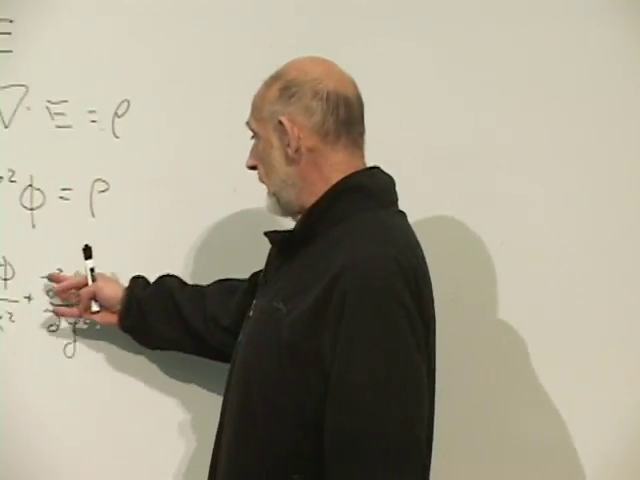
\includegraphics[width=0.70\textwidth]{lecture_08_figure_02.png}
  \caption{El par completo de Cauchy--Riemann, incluido el signo relativo negativo.}
  \lectureframe{00:19:48}
  \label{fig:l08-cr-board}
\end{figure}

La clase distingue brevemente términos relacionados. Una función holomorfa en todo el plano complejo finito es entera. Una función meromorfa puede tener polos aislados. Así, \(1/z\) es analítica salvo en \(z=0\), pero no es entera.

\section{Conjugadas armónicas y geometría conforme}

Las ecuaciones de Cauchy--Riemann son ecuaciones acopladas de primer orden, pero implican ecuaciones separadas de segundo orden. Derivemos \(\partial_xu=\partial_yv\) respecto de \(x\), derivemos \(\partial_yu=-\partial_xv\) respecto de \(y\) y sumemos:
\begin{align}
  \partial_x^2u&=\partial_x\partial_yv,\\
  \partial_y^2u&=-\partial_y\partial_xv,\\
  \therefore\qquad
  \partial_x^2u+\partial_y^2u&=0.
  \label{eq:l08-harmonic-u}
\end{align}
Repitiendo el argumento con \(u\) y \(v\) intercambiadas, se obtiene
\begin{equation}
  \partial_x^2v+\partial_y^2v=0.
  \label{eq:l08-harmonic-v}
\end{equation}
Por tanto, las partes real e imaginaria de una función analítica son conjugadas armónicas. Dos funciones armónicas cualesquiera no forman automáticamente una función analítica: todavía deben estar relacionadas por \eqref{eq:l08-cauchy-riemann}.

\begin{figure}[H]
  \centering
  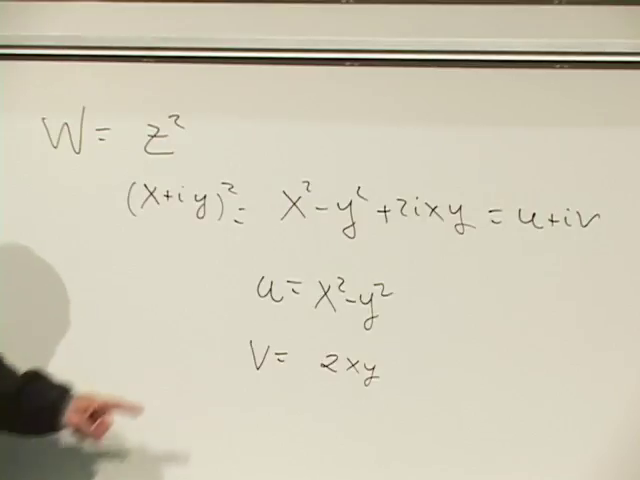
\includegraphics[width=0.68\textwidth]{lecture_08_figure_03.png}
  \caption{Las derivadas mixtas se cancelan y queda la ecuación de Laplace para una componente de la aplicación analítica.}
  \lectureframe{00:23:09}
  \label{fig:l08-harmonic-board}
\end{figure}

También hay una interpretación vectorial útil. Si
\(\mathbf F=(u,-v)\), las dos ecuaciones de Cauchy--Riemann indican, salvo por la convención de orientación elegida, que tanto la divergencia como el rotacional bidimensional de \(\mathbf F\) se anulan. Así volvemos a la electrostática, como se había anunciado.

\subsection{Por qué se conservan los ángulos}

Escribamos dos pequeños desplazamientos complejos en forma polar:
\begin{equation}
  \delta z=\rho e^{i\theta},
  \qquad
  \Delta z=\rho'e^{i\theta'}.
\end{equation}
La fase de su cociente es \(\theta-\theta'\), exactamente el ángulo entre ellos. Bajo una aplicación analítica,
\begin{equation}
  \frac{\delta w}{\delta z}
  =\frac{\Delta w}{\Delta z}
  =w'(z),
\end{equation}
porque la derivada no depende de la dirección. Reordenando, se obtiene
\begin{equation}
  \frac{\Delta z}{\delta z}
  =\frac{\Delta w}{\delta w}.
  \label{eq:l08-angle-ratio}
\end{equation}
Ambos lados tienen la misma fase, así que el ángulo entre los segmentos originales es igual al ángulo entre sus imágenes.

\begin{figure}[H]
  \centering
  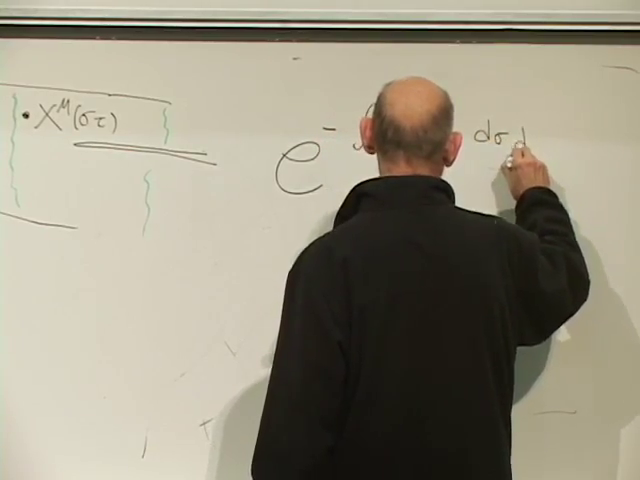
\includegraphics[width=0.70\textwidth]{lecture_08_figure_04.png}
  \medskip

  \begin{tikzpicture}[x=0.9cm,y=0.9cm,>=Latex]
    \begin{scope}
      \draw[->] (-0.2,0) -- (2.3,0);
      \draw[->] (0,-0.2) -- (0,2.1);
      \draw[very thick,blue!65!black,->] (0,0) -- (1.85,0.45)
        node[right] {\(\delta z\)};
      \draw[very thick,orange!75!black,->] (0,0) -- (0.72,1.65)
        node[above] {\(\Delta z\)};
      \draw (0.58,0.14) arc[start angle=14,end angle=66,radius=0.60];
      \node at (1.0,-0.55) {\(z\)-plane};
    \end{scope}
    \draw[->,thick] (3.0,0.9) -- (4.2,0.9)
      node[midway,above] {\(w(z)\)};
    \begin{scope}[xshift=5.0cm]
      \draw[->] (-0.2,0) -- (2.3,0);
      \draw[->] (0,-0.2) -- (0,2.1);
      \draw[very thick,blue!65!black,->] (0,0) -- (1.65,0.70)
        node[right] {\(\delta w\)};
      \draw[very thick,orange!75!black,->] (0,0) -- (0.48,1.62)
        node[above] {\(\Delta w\)};
      \draw (0.54,0.23) arc[start angle=23,end angle=74,radius=0.59];
      \node at (1.0,-0.55) {\(w\)-plane};
    \end{scope}
  \end{tikzpicture}
  \caption{La demostración de la pizarra y una reconstrucción local ordenada. La multiplicación por \(w'(z)\) hace girar y cambiar de escala todas las direcciones infinitesimales en la misma medida, preservando sus ángulos relativos.}
  \lectureframe{00:34:11}
  \label{fig:l08-angle-proof}
\end{figure}

Este argumento local supone que \(w'(z)\neq0\). En un punto crítico, la aplicación puede dejar de ser localmente biyectiva y hay que tratar la geometría por separado. Fuera de esos puntos, las aplicaciones analíticas y las aplicaciones conformes que preservan la orientación son localmente los mismos objetos.

\section{Ejemplos para entrenar la intuición}

\subsection{El cuadrado y la conjugación compleja}

Para \(w=z^2\),
\begin{equation}
  (x+iy)^2=x^2-y^2+2ixy=u+iv,
\end{equation}
por tanto,
\begin{equation}
  u=x^2-y^2,
  \qquad
  v=2xy.
  \label{eq:l08-z-squared-components}
\end{equation}
Las segundas derivadas de \(u\) son \(2\) y \(-2\); las de \(v\) se anulan por separado. Ambas funciones son armónicas, y la derivación directa también verifica las ecuaciones de Cauchy--Riemann.

\begin{figure}[H]
  \centering
  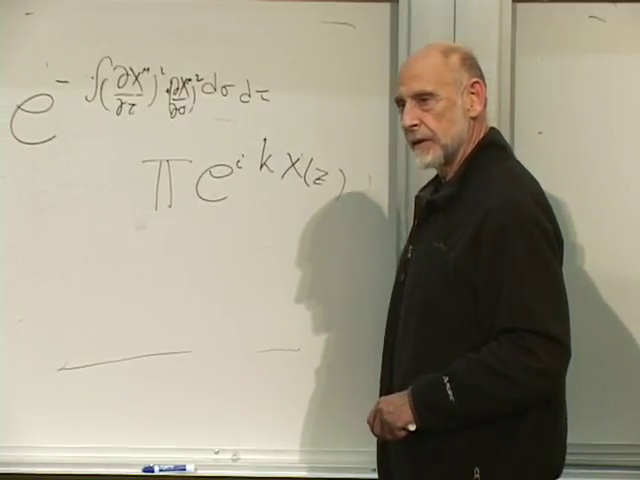
\includegraphics[width=0.72\textwidth]{lecture_08_figure_05.png}
  \caption{La aplicación cuadrática descompuesta en sus componentes armónicas real e imaginaria.}
  \lectureframe{00:36:45}
  \label{fig:l08-z-square-board}
\end{figure}

\begin{classroomqa}
\audiencequestion{¿Da \(1/z\) un ejemplo de función no analítica?
\lecturetimestamp{00:37:49}}
\lecturerresponse{Solo en un punto. Es analítica donde \(z\neq0\) y tiene un polo en el origen. Para ver una aplicación que no supere la prueba de Cauchy--Riemann en ningún punto, la conjugación compleja es un ejemplo más adecuado.}
\end{classroomqa}

En cambio,
\begin{equation}
  w=\bar z=x-iy
  \qquad\Longrightarrow\qquad
  u=x,\quad v=-y
\end{equation}
invierte la orientación. Sus derivadas incumplen por un signo la primera ecuación de Cauchy--Riemann, así que no es analítica como función de \(z\).

\begin{figure}[H]
  \centering
  \includegraphics[width=0.62\textwidth]{lecture_08_figure_06.png}
  \caption{La conjugación compleja ofrece el contraejemplo deliberadamente no analítico.}
  \lectureframe{00:38:38}
  \label{fig:l08-conjugate-board}
\end{figure}

\subsection{La exponencial y su inversa}

\begin{classroomqa}
\audiencequestion{Si \(e^z\) es analítica, ¿por qué también debería ser analítica su inversa \(\log z\)? \lecturetimestamp{00:40:38}}
\lecturerresponse{Donde existe la inversa y \(w'(z)\neq0\), su derivada es \(1/w'(z)\). Por tanto, se conserva la independencia respecto de la dirección. Globalmente, el logaritmo es multivaluado, así que se elige una rama y se excluyen su punto de ramificación y su corte. La afirmación local sobre la conformidad sigue siendo válida en el dominio elegido.}
\end{classroomqa}

La fórmula de Euler da
\begin{equation}
  w=e^z=e^{x+iy}
  =e^x(\cos y+i\sin y),
\end{equation}
y, por tanto,
\begin{equation}
  u=e^x\cos y,
  \qquad
  v=e^x\sin y.
  \label{eq:l08-exponential-components}
\end{equation}
Por ejemplo,
\(\partial_xu=e^x\cos y=\partial_yv\), y la segunda ecuación de Cauchy--Riemann se deduce con la misma facilidad.

\begin{figure}[H]
  \centering
  \includegraphics[width=0.68\textwidth]{lecture_08_figure_07.png}
  \caption{Las componentes real e imaginaria de la aplicación exponencial.}
  \lectureframe{00:42:23}
  \label{fig:l08-exponential-board}
\end{figure}

\section{Semiplano, franja, cilindro y disco}

\subsection{El logaritmo convierte el radio en tiempo}

Tomemos el semiplano derecho, donde
\(-\pi/2<\theta<\pi/2\), y escribamos
\begin{equation}
  z=re^{i\theta},
  \qquad
  w=\log z=\log r+i\theta.
  \label{eq:l08-log-map}
\end{equation}
El semiplano se transforma en la franja infinita
\begin{equation}
  -\frac{\pi}{2}<\operatorname{Im}w<\frac{\pi}{2}.
\end{equation}
Los rayos de \(\theta\) fijo se convierten en rectas horizontales, mientras que las semicircunferencias de \(r\) fijo se convierten en rectas verticales. El origen se transforma en \(\operatorname{Re}w=-\infty\), y \(r=\infty\) en \(\operatorname{Re}w=+\infty\).

\begin{figure}[H]
  \centering
  \includegraphics[width=0.75\textwidth]{lecture_08_figure_08.png}
  \caption{El logaritmo lleva el semiplano derecho a una franja infinita: los rayos polares y las semicircunferencias forman una cuadrícula rectangular ortogonal.}
  \lectureframe{00:47:48}
  \label{fig:l08-log-strip-board}
\end{figure}

La franja es la hoja de universo estándar de una cuerda abierta. Su coordenada acotada parametriza la cuerda, mientras que la traslación a lo largo de la dirección no acotada es el tiempo de la hoja de universo. Bajo la aplicación exponencial inversa, una traslación temporal se convierte en una dilatación \(z\mapsto e^a z\). Así, la misma simetría aparece como una traslación en la franja y como una expansión uniforme en el semiplano.

\begin{classroomqa}
\audiencequestion{¿Adónde va un valor particular como \(r=1\), y siguen siendo polares las coordenadas de la franja? \lecturetimestamp{00:50:58}}
\lecturerresponse{Un círculo de radio fijo se convierte en una recta vertical en \(\operatorname{Re}w=\log r\); en particular, \(r=1\) se transforma en la recta central \(\operatorname{Re}w=0\). Las coordenadas polares describen el plano \(z\). El plano \(w\) usa coordenadas rectangulares ordinarias \((\log r,\theta)\).}
\end{classroomqa}

Si se transforma todo el plano perforado mediante \(\log z\), la coordenada angular tiene período \(2\pi\). Por tanto, los bordes superior e inferior de la franja resultante quedan identificados: es un cilindro infinito. El semiplano con frontera describe la hoja de universo de una cuerda abierta; el plano completo, sin frontera y con ángulo periódico, describe un cilindro de cuerda cerrada.

\begin{figure}[H]
  \centering
  \includegraphics[width=0.75\textwidth]{lecture_08_figure_09.png}
  \caption{La representación del semiplano como franja y la identificación periódica que convierte el plano perforado completo en un cilindro de cuerda cerrada.}
  \lectureframe{00:54:23}
  \label{fig:l08-open-closed-board}
\end{figure}

\subsection{Una aplicación de Cayley al disco unidad}

Una aplicación fraccional lineal, o de Möbius, transforma el semiplano derecho en el disco unidad:
\begin{equation}
  w=\frac{z-1}{z+1}.
  \label{eq:l08-cayley}
\end{equation}
Envía \(z=0\) a \(-1\), \(z=\infty\) a \(+1\) y el eje imaginario a \(|w|=1\). Si \(z=ir\),
\begin{equation}
  \left|\frac{ir-1}{ir+1}\right|=1.
\end{equation}
Los puntos con \(\operatorname{Re}z>0\) quedan dentro del círculo; el semiplano izquierdo se transforma en el exterior.
\editorialnote{Durante la derivación en directo se escribe el recíproco \((z+1)/(z-1)\) al describir la imagen interior del disco. Ese recíproco tiene la misma frontera, la circunferencia unidad, pero envía el semiplano derecho al exterior. La ecuación \eqref{eq:l08-cayley} corresponde a la convención del disco interior, coherente con la geometría descrita.}

\begin{figure}[H]
  \centering
  \includegraphics[width=0.72\textwidth]{lecture_08_figure_10.png}
  \caption{Construcción fraccional lineal de la frontera de la circunferencia unidad. La convención recíproca que aparece en la pizarra intercambia el interior y el exterior.}
  \lectureframe{00:58:38}
  \label{fig:l08-cayley-board}
\end{figure}

Las aplicaciones de Möbius envían la familia generalizada de círculos y rectas a círculos y rectas. Por consiguiente, la cuadrícula radial y circular del semiplano se convierte en dos familias ortogonales de arcos en el disco. Un diámetro recto es simplemente el caso límite de un círculo cuyo centro se ha alejado hasta el infinito.

\begin{classroomqa}
\audiencequestion{¿Son realmente círculos los arcos dibujados dentro del disco?
\lecturetimestamp{01:00:55}}
\lecturerresponse{Sí. Sus centros están en distintas posiciones, a menudo fuera del disco visible. El diámetro es el límite de radio infinito de la misma familia.}
\end{classroomqa}

\begin{classroomqa}
\audiencequestion{¿El dibujo del disco significa que es una esfera? ¿Y adónde va la otra mitad del semiplano? \lecturetimestamp{01:01:21}}
\lecturerresponse{El dibujo es un disco plano, no una esfera. El semiplano derecho se transforma en el interior de su frontera y el semiplano izquierdo, en el exterior. Si se añade el punto del infinito al plano complejo completo, ese plano extendido puede representarse como una esfera mediante proyección estereográfica; se trata de una afirmación global distinta.}
\end{classroomqa}

\begin{classroomqa}
\audiencequestion{¿Qué curvas del disco corresponden a los radios y a las semicircunferencias de radio constante originales? \lecturetimestamp{01:02:59}}
\lecturerresponse{El eje real positivo se convierte en el diámetro que une \(-1\) y \(+1\). Los demás rayos se convierten en arcos circulares que unen esos mismos puntos de la frontera. Las semicircunferencias de radio fijo se convierten en la familia ortogonal que empieza y termina en la circunferencia unidad.}
\end{classroomqa}

\begin{figure}[H]
  \centering
  \includegraphics[width=0.72\textwidth]{lecture_08_figure_11.png}
  \caption{Las rectas y semicircunferencias del semiplano se convierten en familias ortogonales de círculos y rectas en el disco.}
  \lectureframe{01:03:48}
  \label{fig:l08-circle-grid-board}
\end{figure}

\section{La hoja de universo de cuatro cuerdas}

Ahora podemos volver a la dispersión. Entran dos cuerdas abiertas, se unen para formar una sola, esta se propaga durante un intervalo arbitrario y luego se divide en dos cuerdas salientes. En coordenadas de franja, la hoja de universo parece una cinta larga con una abertura en cada extremo---, como una «venda deportiva». La duración de la propagación intermedia no se fija de antemano. Es una de las historias sobre las que se integra la amplitud.

Sean \((\sigma,\tau)\) las coordenadas de la hoja de universo, y sea
\begin{equation}
  X^\mu=X^\mu(\sigma,\tau)
  \label{eq:l08-embedding}
\end{equation}
la posición de esta en el espacio-tiempo. Los índices \(\sigma,\tau\) corresponden a la superficie paramétrica bidimensional; el índice \(\mu\) señala las coordenadas del espacio-tiempo. En la teoría bosónica, \(\mu=0,\ldots,25\); en el caso de las supercuerdas hay diez coordenadas del espacio-tiempo.

Tras la rotación de Wick, los campos libres de incrustación tienen acción euclídea
\begin{equation}
  S_E[X]
  =\frac{1}{4\pi\alpha'}\int_\Sigma d\sigma\,d\tau\,
  \left[
    \partial_\tau X^\mu\partial_\tau X_\mu
    +\partial_\sigma X^\mu\partial_\sigma X_\mu
  \right].
  \label{eq:l08-euclidean-action}
\end{equation}
La integral de camino correspondiente suma todas las incrustaciones posibles de la hoja de universo elegida en el espacio-tiempo:
\begin{equation}
  \int\mathcal D X\,e^{-S_E[X]}.
  \label{eq:l08-bare-worldsheet-integral}
\end{equation}

\begin{figure}[H]
  \centering
  \includegraphics[width=0.74\textwidth]{lecture_08_figure_12.png}
  \caption{El peso euclídeo positivo completo de la hoja de universo. Los dos términos con derivadas se suman sobre todas las componentes del espacio-tiempo.}
  \lectureframe{01:11:34}
  \label{fig:l08-action-board}
\end{figure}

La franja con aberturas tiene una sola frontera conexa. Por tanto, la libertad conforme permite representarla como un disco. Los cuatro extremos lejanos de las franjas se convierten en cuatro puntos marcados en la frontera. Al deformar esos puntos cambia la separación aparente entre la unión y la división en las coordenadas de franja, pero no cambian la superficie subyacente ni la física.

\begin{figure}[H]
  \centering
  \includegraphics[width=0.76\textwidth]{lecture_08_figure_13.png}
  \caption{La hoja de universo en forma de franja con aberturas y su representación como disco, con puntos en la frontera para las cuerdas externas.}
  \lectureframe{01:15:18}
  \label{fig:l08-bandage-disc-board}
\end{figure}

Las líneas detalladas de la cuadrícula que se usan para representar este mapa conforme no tienen contenido físico. Lo que importa es la topología, la frontera y los puntos externos marcados. La misma hoja de universo puede estirarse para mostrar distintos canales sin introducir una interacción nueva.

\section{Estados externos como inserciones en la frontera}

La integral básica \eqref{eq:l08-bare-worldsheet-integral} aún no indica qué momentos entran y cuáles salen. Para un estado escalar de cuerda abierta con momento \(k_i^\mu\), insertemos en la frontera el operador de vértice
\begin{equation}
  V_i(z_i)=e^{\,i k_i\cdot X(z_i)},
  \qquad
  k_i\cdot X=k_{i\mu}X^\mu.
  \label{eq:l08-vertex}
\end{equation}
El punto \(z_i\) es una posición en la frontera de la hoja de universo. No es una coordenada del espacio-tiempo ni una dirección del momento.

\begin{figure}[H]
  \centering
  \includegraphics[width=0.72\textwidth]{lecture_08_figure_14.png}
  \caption{El peso euclídeo del volumen y el producto de las inserciones de momento en la frontera se muestran como factores distintos.}
  \lectureframe{01:18:58}
  \label{fig:l08-vertex-board}
\end{figure}

Para \(n\) cuerdas abiertas externas, la prescripción esquemática es
\begin{equation}
  \begin{aligned}
    \mathcal A_n(k_1,\ldots,k_n)
    &=\int_{\mathcal M_{0,n}^{\partial}}\!d\mu(z_i)
      \int\mathcal D X\\
    &\quad\times e^{-S_E[X]}
      \prod_{i=1}^{n}e^{\,i k_i\cdot X(z_i)}.
  \end{aligned}
  \label{eq:l08-open-string-prescription}
\end{equation}
La integral funcional se toma sobre las incrustaciones \(X^\mu\). La integral de dimensión finita recorre las posiciones de inserción no equivalentes en la frontera. En esta etapa se omiten los factores de polarización y la medida de fijación del gauge, como en la clase.
\editorialnote{Una amplitud de cuerda completa con el gauge fijado contiene también la contribución de los fantasmas correspondiente, factores de vértice que dependen del estado, constantes de acoplamiento y la normalización. La ecuación \eqref{eq:l08-open-string-prescription} recoge la dependencia de los campos de incrustación y de las posiciones que se desarrolla en esta clase.}

\begin{classroomqa}
\audiencequestion{Si los momentos externos están fijados, ¿por qué se integran? \lecturetimestamp{01:20:42}}
\lecturerresponse{No se integran. Los \(k_i\) son etiquetas fijas de la amplitud de dispersión. Lo que se integra son los campos de incrustación y las posiciones \(z_i\) de la hoja de universo en las que se insertan esos momentos fijos. Esta última integral sustituye a la integral sobre la duración de la propagación intermedia en la representación de franja.}
\end{classroomqa}

\begin{classroomqa}
\audiencequestion{¿El producto de factores de vértice está dentro de la integral de camino y forma parte de la acción? \lecturetimestamp{01:21:39}}
\lecturerresponse{Multiplica a \(e^{-S_E}\) dentro de la integral funcional. De manera equivalente, se pueden exponenciar los factores y considerarlos términos fuente localizados que se añaden a la acción, pero conceptualmente son operadores de vértice, no parte de la acción libre del volumen.}
\end{classroomqa}

\begin{figure}[H]
  \centering
  \includegraphics[width=0.76\textwidth]{lecture_08_figure_15.png}
  \caption{La integral de camino escrita con factores separados \(e^{ik_i\cdot X(z_i)}\) para las partículas externas sucesivas.}
  \lectureframe{01:23:23}
  \label{fig:l08-full-prescription-board}
\end{figure}

\begin{classroomqa}
\audiencequestion{¿Por qué \(e^{ik\cdot X}\) sigue conteniendo \(i\) después de la rotación de Wick de la hoja de universo? \lecturetimestamp{01:23:42}}
\lecturerresponse{La rotación cambia el tiempo de la hoja de universo y convierte el peso del volumen de \(e^{iS}\) en \(e^{-S_E}\). El \(i\) de una autofunción de momento es la fase de Fourier que etiqueta el momento del espacio-tiempo. Cumple una función distinta y permanece.}
\end{classroomqa}

\begin{classroomqa}
\audiencequestion{¿La posición \(z_i\) determina la dirección del vector momento? \lecturetimestamp{01:24:19}}
\lecturerresponse{No. La dirección está codificada en las componentes del espacio-tiempo \(k_i^\mu\). El punto de inserción \(z_i\) indica dónde entra ese momento en la descripción de la hoja de universo; \(X^\mu(z_i)\) es uno de los valores del campo sobre los que se suma en \(\mathcal D X\).}
\end{classroomqa}

\begin{classroomqa}
\audiencequestion{¿Los ángulos dibujados de las patas de la venda codifican las direcciones de los momentos físicos? \lecturetimestamp{01:25:07}}
\lecturerresponse{No. La venda representa el espacio de parámetros, no una imagen de la cuerda en el espacio-tiempo físico. Sus patas pueden dibujarse horizontales, inclinadas o deformadas conformemente. Las direcciones físicas las llevan las componentes \(k^\mu\), mientras que \(X^\mu(\sigma,\tau)\) se integra.}
\end{classroomqa}

\section{La integral gaussiana como electrostática}

La acción \eqref{eq:l08-euclidean-action} es cuadrática en cada componente \(X^\mu\), y las inserciones actúan como fuentes lineales una vez que sus exponenciales se combinan con la acción. Por tanto, la integral funcional es gaussiana. En su punto de silla, cada componente del espacio-tiempo satisface una ecuación de Poisson de la forma esquemática
\begin{equation}
  \nabla^2 X^\mu(z)
  \propto
  i\alpha'\sum_i k_i^\mu\,\delta(z-z_i),
  \label{eq:l08-electrostatic-source}
\end{equation}
con la condición de contorno de cuerda abierta en el borde del disco. Cada \(X^\mu\) se comporta como un potencial electrostático independiente, y cada componente del momento \(k_i^\mu\), como la carga correspondiente situada en \(z_i\).

\begin{figure}[H]
  \centering
  \includegraphics[width=0.76\textwidth]{lecture_08_figure_16.png}
  \caption{El disco con fuentes en la frontera se interpreta como un problema electrostático bidimensional independiente para cada componente del espacio-tiempo.}
  \lectureframe{01:28:58}
  \label{fig:l08-electrostatic-disc-board}
\end{figure}

Resolvemos el problema electrostático, calculamos su energía, exponenciamos la energía negativa y, por último, integramos sobre las posiciones de las cargas no equivalentes. Con la normalización estándar de las cuerdas abiertas, el correlador de los campos de incrustación proporciona el factor de Koba--Nielsen
\begin{equation}
  \left\langle\prod_i e^{\,ik_i\cdot X(z_i)}\right\rangle
  \propto
  (2\pi)^D\delta^{(D)}\!\left(\sum_i k_i\right)
  \prod_{i<j}|z_i-z_j|^{2\alpha' k_i\cdot k_j}.
  \label{eq:l08-koba-nielsen}
\end{equation}
La delta de Dirac expresa la conservación del momento. El producto contiene las energías electrostáticas de pares. Para las cuatro inserciones escalares en la frontera que se usan aquí, fijar tres posiciones convierte la integral restante en la integral beta de Euler que apareció en las clases anteriores.

\begin{classroomqa}
\audiencequestion{¿Hay veintiséis energías electrostáticas o solo una?
\lecturetimestamp{01:30:53}}
\lecturerresponse{Hay un potencial y un campo independientes para cada componente del espacio-tiempo. En una base ortonormal del espacio de destino, sus energías cuadráticas no tienen términos cruzados, y las contribuciones se suman para formar una única acción total antes de exponenciarla.}
\end{classroomqa}

\begin{classroomqa}
\audiencequestion{¿La coordenada angular del disco es el ángulo de dispersión físico? \lecturetimestamp{01:32:10}}
\lecturerresponse{No. Es un parámetro de posición en la hoja de universo. Su combinación no equivalente está relacionada con el intervalo de propagación intermedia y se integra. El ángulo de dispersión físico se codifica mediante invariantes de Lorentz construidos a partir de los momentos fijos.}
\end{classroomqa}

\begin{classroomqa}
\audiencequestion{¿Por qué falla esta construcción fuera de la dimensión crítica? \lecturetimestamp{01:32:35}}
\lecturerresponse{Las integrales gaussianas formales por sí solas no constituyen toda la condición de consistencia. La fijación del gauge introduce una anomalía conforme cuyas contribuciones de materia y de fantasmas solo se cancelan en la dimensión crítica: \(D=26\) para la cuerda bosónica y \(D=10\) para la supercuerda. Sin esa cancelación, se pierde la supuesta simetría conforme de la hoja de universo cuántica.}
\end{classroomqa}

\begin{classroomqa}
\audiencequestion{¿Ya hemos supuesto que hay tres dimensiones espaciales grandes y dimensiones extra compactas? \lecturetimestamp{01:33:38}}
\lecturerresponse{No. La compactificación aún no interviene en esta construcción. En esta etapa, las coordenadas bosónicas siguen abarcando las veintiséis direcciones del espacio de destino, o diez en el caso de la supercuerda. La cuestión de cómo un subconjunto puede permanecer macroscópicamente grande se aborda en la siguiente discusión.}
\end{classroomqa}

\begin{classroomqa}
\audiencequestion{¿La conexión con la electrostática consiste simplemente en que las coordenadas satisfacen la ecuación de Laplace? \lecturetimestamp{01:33:57}}
\lecturerresponse{Exactamente. Fuera de los puntos de inserción, cada \(X^\mu\) es armónica; los operadores de vértice aportan fuentes delta de Dirac. Matemáticamente, es el mismo problema de contorno que el de un potencial bidimensional estático con cargas puntuales, usemos o no el vocabulario electrostático.}
\end{classroomqa}

\subsection{Redundancia conforme y número de módulos}

El disco tiene un grupo de automorfismos conformes de tres parámetros reales,
\(\mathrm{PSL}(2,\mathbb R)\). Por tanto, se pueden fijar tres puntos ordenados de la frontera en posiciones convenientes. Para cuatro cuerdas externas, solo queda integrar la cuarta posición; para \(n\) inserciones ordenadas en la frontera, quedan
\begin{equation}
  n-3
  \label{eq:l08-n-minus-three}
\end{equation}
integrales sobre posiciones reales a nivel árbol.

\begin{classroomqa}
\audiencequestion{¿Hay cuatro posiciones angulares independientes alrededor del disco? \lecturetimestamp{01:34:37}}
\lecturerresponse{No desde el punto de vista físico. Al principio se escriben cuatro posiciones, pero la simetría conforme del disco permite situar tres donde convenga. Para la amplitud de dos cuerdas entrantes y dos salientes, solo queda la posición relativa de la cuarta.}
\end{classroomqa}

\begin{figure}[H]
  \centering
  \includegraphics[width=0.72\textwidth]{lecture_08_figure_17.png}
  \caption{Cuatro inserciones en la frontera del disco. La libertad conforme fija tres cualesquiera y deja un módulo para el caso de cuatro puntos.}
  \lectureframe{01:35:18}
  \label{fig:l08-fix-three-board}
\end{figure}

\begin{classroomqa}
\audiencequestion{¿Y si los dos puntos de división no aparecen a la misma altura en el dibujo de la franja? \lecturetimestamp{01:35:24}}
\lecturerresponse{Una aplicación conforme puede eliminar esa diferencia aparente. Los distintos dibujos son representantes en distintas coordenadas del mismo módulo. La integral invariante es la que se toma sobre la posición restante en la frontera, equivalente a la que se toma sobre el intervalo de propagación.}
\end{classroomqa}

\begin{classroomqa}
\audiencequestion{Para más partículas externas, ¿cuántos parámetros de posición quedan? \lecturetimestamp{01:36:00}}
\lecturerresponse{Se fijan tres puntos de inserción mediante la simetría conforme y se integran los otros \(n-3\). Este es el recuento de módulos de frontera para una amplitud de cuerda abierta ordenada a nivel árbol.}
\end{classroomqa}

\begin{classroomqa}
\audiencequestion{¿Qué relación tiene esto con la teoría M?
\lecturetimestamp{01:36:37}}
\lecturerresponse{Aún ninguna. La construcción que hemos visto corresponde a la dispersión perturbativa de cuerdas abiertas en una hoja de universo. Su relación con la teoría M requiere ideas posteriores de dualidad y no perturbativas, así que la cuestión se deja explícitamente para más adelante.}
\end{classroomqa}

\begin{classroomqa}
\audiencequestion{¿Una imagen distinta de la tira vertical o cruzada corresponde a un cálculo distinto? \lecturetimestamp{01:36:49}}
\lecturerresponse{No. Se puede fijar un punto conveniente y dejar que el módulo restante recorra todo su intervalo. Las imágenes de las tiras y la integral sobre los puntos de contorno del disco son distintas foliaciones de una misma integral; por eso se pueden tratar simétricamente todas las cuerdas externas.}
\end{classroomqa}

\section{Lo que la prescripción aún no resuelve}

La fórmula del disco se extiende de inmediato a más cuerdas externas: se añaden más operadores de vértice y se integran sus \(n-3\) posiciones de contorno no equivalentes. Es una prescripción precisa a nivel de árbol para un modelo de cuerdas consistente, pero aún no constituye un modelo realista de la física de partículas observada. La teoría bosónica simple tiene una dimensión espaciotemporal incorrecta y otros defectos físicos. Las supercuerdas mejoran el espectro y reducen la dimensión crítica a diez, pero aún hay que compactificar seis dimensiones espaciales.

\begin{classroomqa}
\audiencequestion{¿Este modelo simple ya concuerda con los experimentos de colisiones de partículas? \lecturetimestamp{01:39:06}}
\lecturerresponse{No. Históricamente, la estructura de resonancias se asemeja a la dispersión hadrónica, pero el modelo bosónico de veintiséis dimensiones no puede describir directamente las partículas observadas. El formalismo define amplitudes de dispersión para el modelo; para concordar con la naturaleza se necesitan un espectro realista, compactificación, interacciones y una elección del vacío.}
\end{classroomqa}

\begin{classroomqa}
\audiencequestion{¿La compactificación reducirá las dimensiones adicionales y producirá datos realistas sobre partículas? \lecturetimestamp{01:41:10}}
\lecturerresponse{Puede reducir la dimensión macroscópica efectiva y generar espectros de partículas y grupos gauge. También es donde entra buena parte de la verdadera dificultad matemática. Se conocen muchas compactificaciones consistentes, y sigue sin resolverse cómo seleccionar un modelo único de las partículas elementales observadas.}
\end{classroomqa}

La clase hace hincapié en esta distinción, en lugar de presentar la teoría como si estuviera terminada. Las construcciones de cuerdas están definidas matemáticamente y han proporcionado información profunda sobre la gravedad y la geometría; sin embargo, su multiplicidad forma parte del propio problema físico.

\begin{classroomqa}
\audiencequestion{¿Hay una forma breve de recordar por qué la dimensión crítica bosónica es veintiséis? \lecturetimestamp{01:43:19}}
\lecturerresponse{En el cálculo anterior de los osciladores se usó la suma regularizada de energías de punto cero \(1+2+3+\cdots=-1/12\). La contribución de los osciladores transversales comprende veinticuatro direcciones, y al restituir las dos coordenadas espaciotemporales longitudinales se obtiene \(24+2=26\). Es una regla mnemotécnica para el argumento de consistencia anterior, no una derivación nueva aquí.}
\end{classroomqa}

\begin{classroomqa}
\audiencequestion{¿Están cuantizados los momentos insertados \(k_i\)? \lecturetimestamp{01:43:46}}
\lecturerresponse{En un espaciotiempo no compacto, sus componentes son continuas. Lo que está cuantizado es el nivel de los osciladores y, por tanto, el espectro permitido de masa al cuadrado. Las dimensiones compactas pueden cuantizar las componentes correspondientes del momento y del número de enrollamiento, pero eso se aborda en la siguiente discusión.}
\end{classroomqa}

\chapter{Cuerdas, gravedad, compactificación y dualidad T}

\lectureoverview{Una partícula puntual puede moverse de manera coherente en prácticamente cualquier geometría suave, pero una cuerda cuántica no. Sus infinitas oscilaciones de punto cero sondean el espacio objetivo a escalas cada vez menores, y la geometría efectiva cambia a medida que se restituyen esas oscilaciones. Exigir que este proceso tenga un punto fijo conduce a \(R_{\mu\nu}=0\), la ecuación de Einstein en el vacío. Luego pasamos de esta condición de coherencia a la compactificación. Un círculo proporciona tanto estados de momento de Kaluza--Klein como estados de enrollamiento de la cuerda; intercambiarlos identifica un círculo de radio \(R\) con otro de radio \(\alpha'/R\).}

\section{La coherencia como principio de selección}

Hay dos preguntas que responder. ¿Por qué aparece la gravedad en la teoría de cuerdas y por qué esta es mucho menos permisiva que la mecánica de partículas puntuales? En realidad, son una sola pregunta. Una geometría de fondo es admisible únicamente si una cuerda puede propagarse en ella sin conservar una dependencia arbitraria de la resolución con la que la describimos.

Empecemos por el problema de control: una partícula puntual restringida a una superficie curva y suave. Clásicamente, sigue una geodésica, el análogo intrínseco de una línea recta. Se puede aproximar el movimiento mediante muchos segmentos cortos, escribir una ecuación en diferencias y luego hacer tender a cero la longitud de los segmentos. El resultado es una ecuación diferencial ordinaria con un límite continuo bien definido.

La mecánica cuántica modifica la suma sobre historias, pero no la conclusión. En vez de seleccionar una trayectoria clásica, sumamos las amplitudes de las trayectorias sobre la superficie. También aquí se puede dividir el tiempo en pasos pequeños; el límite se describe de forma equivalente mediante una ecuación de Schr\"odinger en el espacio de configuraciones curvo. Para una superficie suave, el límite conduce a un propagador y un espectro definidos.

\begin{figure}[H]
  \centering
  \includegraphics[width=0.72\textwidth]{lecture_09_figure_01.png}
  \caption{Una trayectoria suave sobre la superficie y una trayectoria irregular de la suma cuántica discretizada en el tiempo. Ambas permanecen en la superficie objetivo.}
  \lectureframe{00:05:10}
  \label{fig:l09-particle-paths}
\end{figure}

\begin{classroomqa}
\audiencequestion{En la integral de camino, ¿todas las trayectorias deben permanecer dentro de la superficie? \lecturetimestamp{00:05:39}}
\lecturerresponse{Sí. La superficie es el espacio de configuraciones de la partícula, no una lámina incrustada en una habitación mayor por la que la partícula pueda tomar un atajo. Cada punto intermedio pertenece a la superficie, y todas las longitudes y acciones se calculan con su métrica intrínseca.}
\end{classroomqa}

La pregunta correspondiente para una cuerda es más difícil. Una cuerda no queda especificada solo por la posición de su centro de masa. Tiene una torre infinita de osciladores, de modo que mejorar la resolución significa admitir más grados de libertad dinámicos. La teoría solo es coherente si los observables convergen a un límite al restituir esa torre.

\section{La partícula puntual sobre una esfera}

La esfera es la geometría curva de prueba más sencilla. Sea \(R\) su radio y situemos primero sobre ella una partícula de masa \(m\). Para el movimiento a lo largo de un círculo máximo,
\begin{equation}
  E=\frac{1}{2}mv^2=\frac{p^2}{2m},
  \qquad
  L=pR.
  \label{eq:l09-particle-energy}
\end{equation}
Por consiguiente,
\begin{equation}
  E=\frac{L^2}{2mR^2}
   =\frac{L^2}{2I},
  \qquad
  I=mR^2.
  \label{eq:l09-rotor-energy}
\end{equation}
El radio interviene a través del momento de inercia. Al cuantizar el momento angular se obtiene el conocido espectro del rotor rígido, y nada depende de un corte ultravioleta.

\begin{figure}[H]
  \centering
  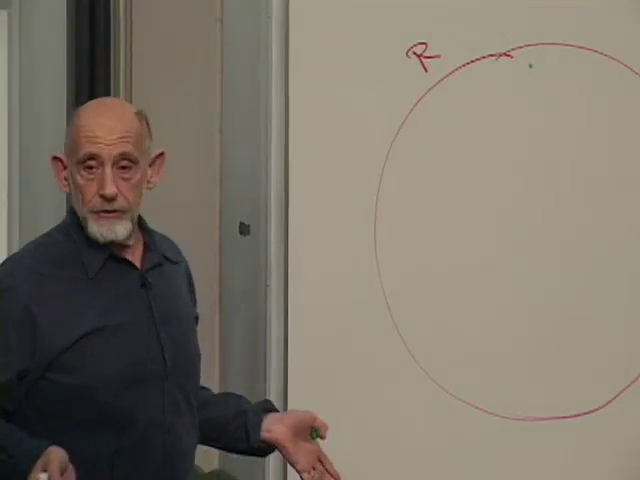
\includegraphics[width=0.74\textwidth]{lecture_09_figure_02.png}
  \caption{El cálculo de control para la partícula puntual:
  \(p^2/(2m)=L^2/(2mR^2)=L^2/(2I)\).}
  \lectureframe{00:11:25}
  \label{fig:l09-sphere-rotor}
\end{figure}

Este ejemplo sin complicaciones es importante. La curvatura por sí sola no es el problema. El problema aparece cuando la curvatura se acopla a la extensión cuántica interna de una cuerda.

\section{La cuerda en el vacío no es puntual}

Consideremos una coordenada transversal de una cuerda abierta y restémosle su centro de masa. La expansión en osciladores que usamos aquí es esquemática:
\begin{equation}
  X(\sigma)-X_{\mathrm{cm}}
  \sim
  \sum_{n=1}^{\infty}
  \frac{a_n+a_n^\dagger}{\sqrt n}\cos(n\sigma).
  \label{eq:l09-mode-expansion}
\end{equation}
Los elementos esenciales son los modos coseno, los operadores de oscilador y el factor \(1/\sqrt n\). Las normalizaciones exactas no influyen en el argumento sobre el tamaño.
\editorialnote{La expansión precisa contiene factores \(\alpha'\) que dependen de las convenciones, constantes numéricas y una elección de notación para los osciladores. La ecuación \eqref{eq:l09-mode-expansion} conserva solo la dependencia necesaria para la estimación ultravioleta, al igual que en la derivación en la pizarra.}

\begin{figure}[H]
  \centering
  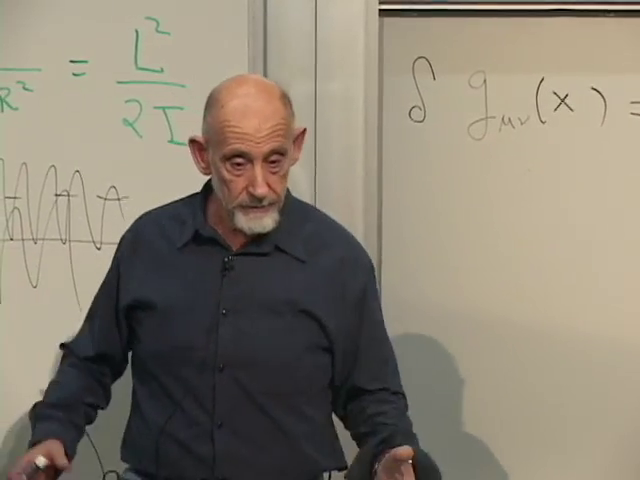
\includegraphics[width=0.78\textwidth]{lecture_09_figure_03.png}
  \caption{La expansión estructural en osciladores y la suma doble que se obtiene al elevarla al cuadrado.}
  \lectureframe{00:15:20}
  \label{fig:l09-string-modes}
\end{figure}

El valor esperado del cuadrado de la distancia al centro de masa en el vacío de osciladores es
\begin{align}
  \expect{\bigl(X(\sigma)-X_{\mathrm{cm}}\bigr)^2}_0
  &\sim
  \sum_{n,m\geq1}
  \frac{\cos(n\sigma)\cos(m\sigma)}{\sqrt{nm}}\notag\\
  &\qquad\times
  \bra{0}(a_n+a_n^\dagger)\notag\\
  &\hspace{6em}\times(a_m+a_m^\dagger)\ket{0}.
  \label{eq:l09-size-double-sum}
\end{align}
La mayoría de los términos se anulan. Dos operadores de aniquilación aniquilan el ket; dos operadores de creación dejan un estado ortogonal al bra; y un operador de creación seguido de uno de aniquilación también tiene valor esperado nulo en el vacío con este orden. La contracción que sobrevive es
\begin{equation}
  \bra{0}a_n a_m^\dagger\ket{0}=\delta_{nm}.
  \label{eq:l09-vacuum-contraction}
\end{equation}

\begin{figure}[H]
  \centering
  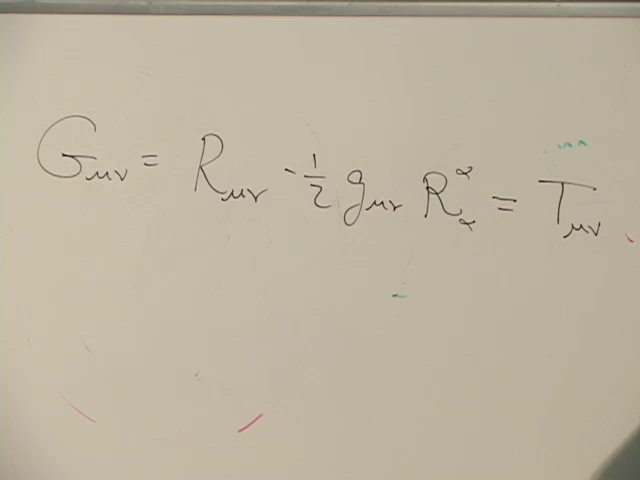
\includegraphics[width=0.74\textwidth]{lecture_09_figure_04.png}
  \caption{La contracción de vacío que sobrevive reduce la suma doble sobre osciladores a una suma simple.}
  \lectureframe{00:20:10}
  \label{fig:l09-vacuum-contraction}
\end{figure}

Así,
\begin{equation}
  \expect{\bigl(X(\sigma)-X_{\mathrm{cm}}\bigr)^2}_0
  \sim
  \sum_{n=1}^{\infty}\frac{\cos^2(n\sigma)}{n}.
  \label{eq:l09-size-single-sum}
\end{equation}
En un punto genérico de la cuerda, o al promediar sobre \(\sigma\), \(\cos^2(n\sigma)\) contribuye aproximadamente \(1/2\). Con un corte en los modos \(N\),
\begin{equation}
  \expect{\bigl(X-X_{\mathrm{cm}}\bigr)^2}_{0,N}
  \sim
  \frac{1}{2}\sum_{n=1}^{N}\frac{1}{n}
  =\frac{1}{2}\log N+O(1).
  \label{eq:l09-logarithmic-size}
\end{equation}

\begin{figure}[H]
  \centering
  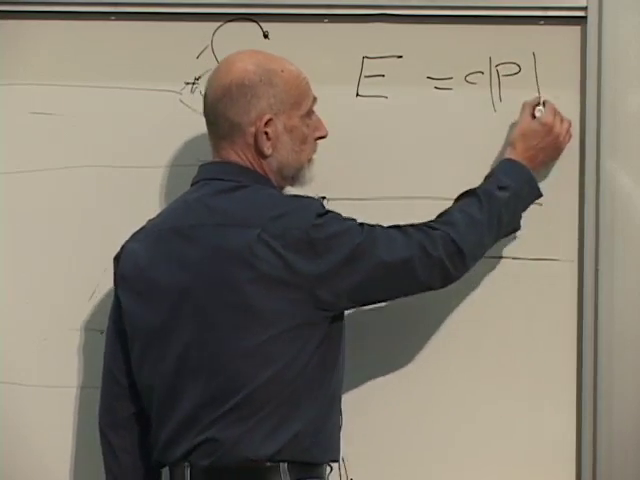
\includegraphics[width=0.72\textwidth]{lecture_09_figure_05.png}
  \caption{En la pizarra se llega a la serie armónica que determina la extensión del estado fundamental.}
  \lectureframe{00:22:05}
  \label{fig:l09-harmonic-size}
\end{figure}

Si se conservan, por ejemplo, solo los primeros veinticinco modos, se obtiene un objeto difuso finito, pero aún no la cuerda continua. Al eliminar el corte, la extensión cuadrática media crece logarítmicamente. No debe interpretarse esta conclusión como una demostración de que la teoría de cuerdas en el espacio plano sea incoherente. En el espacio plano, el movimiento del centro de masa y el de los osciladores se separan, y delicadas cancelaciones en las amplitudes físicas preservan la localidad esperada. El aumento del tamaño es una señal de alerta. La curvatura nos indica si esa señal se convierte en un problema.

\section{Cuando la extensión interna modifica la geometría}

Situemos la cuerda cerca del polo norte de la esfera. Con todos los osciladores apagados, se comporta como la partícula puntual que acabamos de estudiar. A medida que se admiten modos de frecuencia más alta, la cuerda se convierte en un enredo fluctuante que se extiende por el casquete. Su centro puede seguir recorriendo la esfera, pero el objeto cuyo momento de inercia interviene en la energía de rotación ahora tiene extensión.

Para un eje que pasa por el centro de la esfera y por los polos,
\begin{equation}
  I=\int r_\perp^2\,dm,
  \label{eq:l09-extended-inertia}
\end{equation}
donde \(r_\perp\) es la distancia perpendicular entre un elemento de cuerda y ese eje. Un punto del ecuador de la órbita tiene el mayor brazo de palanca pertinente. Las partes de la cuerda que cuelgan hacia el eje contribuyen menos. A masa total fija, esto reduce el momento de inercia efectivo:
\begin{equation}
  I_{\mathrm{eff}}<mR^2.
  \label{eq:l09-inertia-reduction}
\end{equation}
Por tanto, la energía de rotación parece la de un objeto puntual sobre una esfera más pequeña,
\begin{equation}
  E_{\mathrm{rot}}
  =\frac{L^2}{2I_{\mathrm{eff}}}
  \equiv \frac{L^2}{2mR_{\mathrm{eff}}^2},
  \qquad R_{\mathrm{eff}}<R.
  \label{eq:l09-effective-radius}
\end{equation}

\begin{classroomqa}
\audiencequestion{¿Por qué el momento de inercia debería tender a cero si la cuerda se está extendiendo por una región mayor? \lecturetimestamp{00:33:23}}
\lecturerresponse{La afirmación se refiere a la descripción efectiva al efectuar sucesivos promedios a gran escala; no sostiene que la distribución extendida sin promediar tenga de inmediato momento de inercia nulo. La primera banda de modos convierte el punto en una masa difusa que se mueve como si estuviera en una esfera menor. La banda siguiente resuelve la estructura interna de cada una de esas masas y repite la misma renormalización. Al iterar esta comparación, el radio efectivo se reduce.}
\end{classroomqa}

\begin{figure}[H]
  \centering
  \includegraphics[width=0.72\textwidth]{lecture_09_figure_06.png}
  \medskip

  \begin{adjustbox}{max width=\linewidth}
  \begin{tikzpicture}[x=1cm,y=1cm,>=Latex]
    \draw[thick] (0,0) circle (2.15);
    \draw[dashed] (0,-2.55) -- (0,2.55);
    \draw[blue!65!black,thick]
      (-0.22,2.05)
      .. controls (-1.22,1.75) and (-1.52,1.08) .. (-1.06,0.44)
      .. controls (-0.55,-0.10) and (0.35,0.02) .. (1.10,0.68)
      .. controls (1.48,1.12) and (1.16,1.80) .. (0.20,2.05);
    \draw[red!70!black,dashed] (0,0) circle (1.25);
    \draw[->] (2.70,1.55) -- (4.05,1.55);
    \node[align=center] at (3.37,1.98) {add shorter\\modes};
    \draw[thick] (6.15,0) circle (1.25);
    \draw[dashed] (6.15,-1.65) -- (6.15,1.65);
    \draw[blue!65!black,thick]
      (6.00,1.18)
      .. controls (5.42,0.88) and (5.46,0.25) .. (6.02,-0.06)
      .. controls (6.46,-0.28) and (6.90,0.45) .. (6.28,1.18);
    \node at (0,-3.00) {sphere of radius \(R\)};
    \node at (6.15,-2.05) {effective radius \(R_{\mathrm{eff}}\)};
  \end{tikzpicture}
  \end{adjustbox}
\caption{La cuerda cerca del polo norte, tal como aparece en la pizarra, y una reconstrucción clara del argumento del radio efectivo. El círculo interior discontinuo representa una geometría efectiva, no una segunda capa física dentro de la esfera.}
  \lectureframe{00:35:15}
  \label{fig:l09-shrinking-sphere}
\end{figure}

Esto es una afirmación sobre el grupo de renormalización. Con un corte finito, la cuerda es una masa con resolución interna finita. Elevar el corte modifica la mecánica de esa masa. En una esfera de curvatura positiva, cada capa de modos que se añade hace menor el fondo que se infiere a partir del movimiento a larga distancia. Si el resultado nunca se estabiliza, no existe una teoría de cuerdas independiente del corte en ese fondo.

\section{La métrica debe alcanzar un punto fijo}

Sustituyamos ahora la esfera por una métrica general del espacio objetivo \(g_{\mu\nu}(x)\). Integrar una capa logarítmica delgada de modos de oscilador modifica esa métrica mediante un tensor simétrico local de rango dos. La variación debe anularse en el espacio plano y comenzar con dos derivadas de la métrica. A orden dominante, la covariancia deja al tensor de Ricci como candidato pertinente:
\begin{equation}
  \frac{\partial g_{\mu\nu}}{\partial\log\Lambda}
  =-C\,R_{\mu\nu}+\cdots ,
  \qquad C>0
  \label{eq:l09-ricci-flow}
\end{equation}
en el sentido del promedio a gran escala empleado en el argumento geométrico. Así, la curvatura positiva hace que una esfera se contraiga, como se requiere.
\editorialnote{La normalización y el signo dependen de si el parámetro de renormalización aumenta hacia el ultravioleta o hacia el infrarrojo. En la notación convencional de la hoja de universo, la función beta de la métrica a orden dominante es \(\beta^g_{\mu\nu}=\alpha'R_{\mu\nu}+\cdots\). La afirmación invariante que usamos aquí es que la independencia del corte requiere que la función beta, y por tanto \(R_{\mu\nu}\) a este orden, se anule.}

\begin{figure}[H]
  \centering
  \includegraphics[width=0.76\textwidth]{lecture_09_figure_07.png}
  \caption{La variación de la métrica se representa esquemáticamente como menos el tensor de Ricci, junto a una curva que se suaviza.}
  \lectureframe{00:43:00}
  \label{fig:l09-ricci-flow-board}
\end{figure}

\begin{classroomqa}
\audiencequestion{¿Dónde aparece el corte de osciladores \(N\) en esta ecuación de flujo? \lecturetimestamp{00:43:38}}
\lecturerresponse{Es la variable de escala. La suma que determina el tamaño de la cuerda varía logarítmicamente al cambiar el modo de mayor frecuencia incluido, así que el parámetro de evolución natural es \(\log N\), o, de manera equivalente, \(\log\Lambda\). La ecuación \eqref{eq:l09-ricci-flow} describe la variación infinitesimal causada por una capa logarítmica de modos.}
\end{classroomqa}

Un fondo admisible es un punto fijo de este flujo. A orden dominante,
\begin{equation}
  \boxed{R_{\mu\nu}=0.}
  \label{eq:l09-ricci-flat}
\end{equation}
Ser Ricci plano no significa que todas las componentes del tensor de Riemann se anulen. Por ejemplo, las ondas gravitacionales pueden tener curvatura no nula en el vacío y, aun así, satisfacer \(R_{\mu\nu}=0\).

\subsection{La misma condición es la ecuación de Einstein en el vacío}

Con las constantes convencionales suprimidas, la ecuación de Einstein es
\begin{equation}
  G_{\mu\nu}
  \equiv
  R_{\mu\nu}-\frac12 g_{\mu\nu}R
  =T_{\mu\nu}.
  \label{eq:l09-einstein}
\end{equation}

\begin{figure}[H]
  \centering
  \includegraphics[width=0.78\textwidth]{lecture_09_figure_08.png}
  \caption{El tensor de Einstein y el tensor de energía y momento en la pizarra.}
  \lectureframe{00:47:15}
  \label{fig:l09-einstein-board}
\end{figure}

En el vacío, \(T_{\mu\nu}=0\). Tomando la traza en un espacio-tiempo de \(D\) dimensiones se obtiene
\begin{equation}
  0=g^{\mu\nu}G_{\mu\nu}
   =\left(1-\frac{D}{2}\right)R.
  \label{eq:l09-einstein-trace}
\end{equation}
Para \(D\neq2\), \(R=0\), y al sustituir de nuevo en \eqref{eq:l09-einstein} se obtiene \(R_{\mu\nu}=0\). Así, la condición de que la cuerda pierda su dependencia del corte es la ecuación del campo gravitatorio en el vacío. La gravedad no se ha añadido a la teoría; aparece como precio de la coherencia.

La palabra \emph{vacío} no significa que no ocurra nada. Significa que no hay fuentes de energía-momento en la región. Las ecuaciones de Maxwell sin fuentes admiten ondas electromagnéticas, y las ecuaciones de Einstein sin fuentes admiten ondas gravitacionales. La geometría puede ser dinámica aunque su tensor de Ricci se anule.

\begin{classroomqa}
\audiencequestion{¿Está relacionada esta condición con la invariancia conforme?
\lecturetimestamp{00:52:20}}
\lecturerresponse{Sí, aunque la grabación no conserva parte de la pregunta. La simetría pertinente es la invariancia conforme de la teoría cuántica de la \emph{hoja de universo}. Exigir que se anule la anomalía de escala de la hoja de universo es lo que hace que la función beta de la métrica sea cero. No debe confundirse esto con exigir invariancia conforme del propio espacio-tiempo.}
\end{classroomqa}

Hay una segunda condición de coherencia. La invariancia conforme de la hoja de universo también fija la dimensión crítica del espacio-tiempo: diez para las supercuerdas y veintiséis para la cuerda bosónica. Por tanto, la planitud de Ricci no es la lista completa de requisitos, pero sí es la parte que muestra de forma más directa la ecuación de Einstein.

\section{Dimensiones compactas en lugar de dimensiones ausentes}

Un fondo de supercuerdas tiene nueve dimensiones espaciales y una dimensión temporal. Nuestro mundo macroscópico muestra solo tres direcciones espaciales grandes, así que seis dimensiones espaciales deben estar ocultas o ser inaccesibles de algún otro modo a las escalas ordinarias. La compactificación las conserva como direcciones auténticas, pero les asigna una extensión finita pequeña.

\begin{classroomqa}
\audiencequestion{Si distintos observadores llevan relojes distintos, ¿eso equivale a tener más de una dimensión temporal? \lecturetimestamp{00:56:59}}
\lecturerresponse{No. Muchos relojes son muchos instrumentos que miden coordenadas en un solo espacio-tiempo; no crean direcciones temporales independientes. Las dimensiones adicionales que consideramos aquí son espaciales. Las construcciones cuánticas y causales habituales no proporcionan una teoría coherente comparable con varias direcciones temporales locales, así que esa posibilidad no forma parte de este modelo de compactificación.}
\end{classroomqa}

Imaginemos criaturas que creen que su mundo es una línea. A baja resolución, solo pueden moverse hacia delante y hacia atrás. Sin embargo, bajo un microscopio suficientemente potente, se descubre que la línea es un cilindro muy estrecho. Una criatura pequeña puede moverse alrededor de su dirección circular, además de recorrerlo a lo largo. La segunda dirección siempre estuvo presente; su circunferencia era demasiado pequeña para que la detectaran las sondas de baja resolución.

\begin{figure}[H]
  \centering
  \includegraphics[width=0.78\textwidth]{lecture_09_figure_09.png}
  \caption{Un cilindro estrecho y trayectorias que se enrollan alrededor de su dirección circular oculta.}
  \lectureframe{01:01:00}
  \label{fig:l09-hidden-cylinder}
\end{figure}

Un cilindro se puede representar como una franja cuyos bordes superior e inferior están identificados. Al cruzar el borde superior se vuelve por el inferior en la misma posición longitudinal. Ninguno de los bordes es una frontera física. Se puede hacer lo mismo con dos direcciones: se identifican los bordes izquierdo y derecho de un rectángulo, y también sus bordes superior e inferior. El resultado es un toro bidimensional.

\begin{figure}[H]
  \centering
  \includegraphics[width=0.76\textwidth]{lecture_09_figure_10.png}
  \medskip

  \begin{tikzpicture}[x=0.82cm,y=0.82cm,>=Latex]
    \draw[thick] (0,0) rectangle (4,2.15);
    \draw[blue!65!black,->] (0,2.48) -- (4,2.48);
    \draw[blue!65!black,->] (4,-0.34) -- (0,-0.34);
    \node at (2,-0.82) {one periodic direction};
    \draw[thick] (6.1,0) rectangle (10.1,2.15);
    \draw[blue!65!black,->] (6.1,2.48) -- (10.1,2.48);
    \draw[blue!65!black,->] (10.1,-0.34) -- (6.1,-0.34);
    \draw[red!70!black,->] (5.76,0) -- (5.76,2.15);
    \draw[red!70!black,->] (10.44,2.15) -- (10.44,0);
    \node at (8.1,-0.82) {two periodic directions};
  \end{tikzpicture}
  \caption{El prisma de la pizarra y una descripción clara mediante un dominio fundamental. Identificar un par de bordes da un cilindro; identificar ambos pares da un toro.}
  \lectureframe{01:04:40}
  \label{fig:l09-periodic-identification}
\end{figure}

El toro es una topología antes de ser una superficie con forma de rosquilla incrustada en un espacio tridimensional. Si se corta un toro una vez, se convierte en un cilindro; si se vuelve a cortar, se convierte en un rectángulo, siempre que se recuerden las identificaciones de los bordes. Se puede dotar a este rectángulo de una métrica plana; por tanto, el toro plano resultante tiene curvatura de Riemann local nula y, sin duda, es Ricci plano.

Una trayectoria recta en el rectángulo continúa en línea recta al cruzar un borde identificado. Si su pendiente es un cociente racional de los dos períodos, la trayectoria acaba cerrándose. Si el cociente es irracional, nunca se cierra y se vuelve densa en el toro.

\begin{figure}[H]
  \centering
  \includegraphics[width=0.76\textwidth]{lecture_09_figure_11.png}
  \caption{Los segmentos rectos repetidos dentro de un dominio fundamental representan una única trayectoria ininterrumpida sobre el toro.}
  \lectureframe{01:11:00}
  \label{fig:l09-torus-trajectory}
\end{figure}

Los toros de dimensión superior se forman del mismo modo. Un cubo en el que se identifica cada par de caras opuestas es un toro tridimensional, y seis direcciones compactas se pueden modelar mediante un toro de seis dimensiones. No se debe intentar incrustar todos estos objetos en el espacio tridimensional ordinario; la descripción mediante la identificación de caras es intrínseca y completa.

\begin{classroomqa}
\audiencequestion{¿Es necesario que una dimensión adicional se cierre sobre sí misma?
\lecturetimestamp{01:15:03}}
\lecturerresponse{No es un teorema. Podría ser no compacta, pero entonces normalmente aparecería como otra dirección grande en el mundo observado a larga distancia. La compacidad es la forma más sencilla de conciliar las dimensiones adicionales con su aparente ausencia. La razón por la que la naturaleza elige una compactificación concreta es una cuestión dinámica aparte.}
\end{classroomqa}

\begin{classroomqa}
\audiencequestion{¿Por qué suponer que las dimensiones que no vemos son direcciones espaciales ordinarias enrolladas de esta manera y no algo completamente distinto? \lecturetimestamp{01:15:51}}
\lecturerresponse{Porque es una hipótesis concreta y resoluble, no porque se haya demostrado que sea la única descripción de la naturaleza. Las variedades espaciales compactas nos permiten construir ejemplos coherentes y calcular sus espectros. Las posibilidades más exóticas deben demostrar que también pueden hacerlo.}
\end{classroomqa}

\begin{classroomqa}
\audiencequestion{Las distancias en el toro familiar con forma de rosquilla no parecen distancias en un rectángulo. ¿A qué geometría nos referimos?
\lecturetimestamp{01:18:11}}
\lecturerresponse{El término \emph{toro} fija las identificaciones, no una métrica única. La rosquilla incrustada hereda una métrica curva del espacio tridimensional. El rectángulo con identificaciones periódicas tiene una métrica plana. Tienen la misma topología y geometrías distintas; para la compactificación sencilla nos referimos a la plana.}
\end{classroomqa}

\section{Los parámetros de forma de un toro plano}

Ni siquiera un toro plano bidimensional es único. Su paralelogramo fundamental tiene un área total, una razón de aspecto y un sesgo. Cambiar estos parámetros modifica las distancias y, por tanto, el espectro, sin cambiar la topología.

\begin{figure}[H]
  \centering
  \includegraphics[width=0.74\textwidth]{lecture_09_figure_12.png}
  \medskip

  \begin{tikzpicture}[x=0.9cm,y=0.9cm,>=Latex]
    \draw[thick] (0,0) rectangle (3.4,2.1);
    \draw[<->] (0,-0.35) -- node[below] {\(L_1\)} (3.4,-0.35);
    \draw[<->] (-0.35,0) -- node[left] {\(L_2\)} (-0.35,2.1);
    \draw[thick] (5.4,0) -- (8.8,0) -- (9.7,2.1) -- (6.3,2.1) -- cycle;
    \draw[dashed] (5.4,0) -- (6.3,2.1);
    \draw[->] (5.75,2.48) -- node[above] {shear} (6.45,2.48);
    \node at (1.7,-1.00) {area and aspect ratio};
    \node at (7.55,-1.00) {complex structure};
  \end{tikzpicture}
  \caption{Los dominios fundamentales rectangular y sesgado que se usan para analizar los módulos del toro.}
  \lectureframe{01:23:00}
  \label{fig:l09-torus-moduli}
\end{figure}

Para un toro bidimensional, resulta útil representar la forma mediante un número complejo \(\tau=\tau_1+i\tau_2\): la parte real registra el sesgo y la parte imaginaria, la razón de aspecto una vez separado el factor de escala global. Intercambiar los dos ciclos básicos o cambiar su base entera puede hacer que paralelogramos aparentemente diferentes describan el mismo toro.

\begin{classroomqa}
\audiencequestion{¿Qué ocurre si se invierte un borde antes de identificarlo? \lecturetimestamp{01:24:20}}
\lecturerresponse{Eso produce una topología distinta. Identificar mediante una reflexión da lugar a una superficie no orientable, la botella de Klein, en vez de un toro ordinario.}
\end{classroomqa}

\begin{classroomqa}
\audiencequestion{¿Qué ocurre si el giro no es uniforme a lo largo del borde?
\lecturetimestamp{01:25:01}}
\lecturerresponse{Una deformación suave no uniforme se puede incorporar a la métrica del dominio fundamental. Hay que mantener diferenciadas la identificación topológica y los datos geométricos: cambiar la unión puede modificar la topología, mientras que cambiar suavemente las distancias modifica la métrica.}
\end{classroomqa}

\editorialnote{Para un toro plano bidimensional, el área es el módulo de Kähler más sencillo y \(\tau\) es el módulo de la estructura compleja. Un sesgo continuo forma parte de \(\tau\). En cambio, un giro de Dehn es una operación discreta de clase de mapeo, representada por \(\tau\mapsto\tau+1\); no es en sí mismo el módulo continuo. Esto precisa la terminología intencionadamente informal usada durante la discusión en la pizarra.}

Los toros planos son útiles porque satisfacen inmediatamente la condición de coherencia, pero su simetría es demasiado amplia para un modelo realista de física de partículas. Espacios Ricci planos más complejos, en particular las variedades de Calabi--Yau, dan lugar a compactificaciones más ricas. Su construcción detallada queda fuera de esta discusión; el principio es el mismo.

\section{Leer un círculo compacto a partir de su espectro}

Después del descanso, reduzcamos el espacio compacto a un círculo de circunferencia \(2\pi R\). La función de onda debe ser monovaluada después de una vuelta:
\begin{equation}
  e^{ip_c(x+2\pi R)/\hbar}=e^{ip_cx/\hbar}.
\end{equation}
Por tanto,
\begin{equation}
  p_cR=n\hbar,
  \qquad
  p_c=\frac{n\hbar}{R},
  \qquad n\in\mathbb Z.
  \label{eq:l09-kk-momentum}
\end{equation}

\begin{figure}[H]
  \centering
  \includegraphics[width=0.74\textwidth]{lecture_09_figure_13.png}
  \caption{La circunferencia compacta \(2\pi R\) y el momento cuantizado \(p_c=n\hbar/R\).}
  \lectureframe{01:32:15}
  \label{fig:l09-kk-board}
\end{figure}

Para una partícula sin masa en el espacio-tiempo completo,
\begin{equation}
  E=c|\mathbf P|.
  \label{eq:l09-massless-dispersion}
\end{equation}

\begin{figure}[H]
  \centering
  \includegraphics[width=0.70\textwidth]{lecture_09_figure_14.png}
  \caption{La relación de dispersión de la partícula sin masa, usada para reinterpretar el momento compacto como masa en menos dimensiones.}
  \lectureframe{01:33:45}
  \label{fig:l09-massless-board}
\end{figure}

Separemos el momento en sus partes no compacta y compacta, y fijemos \(c=\hbar=1\):
\begin{equation}
  E^2=\mathbf p_{\mathrm{large}}^2+\frac{n^2}{R^2}.
  \label{eq:l09-kk-dispersion}
\end{equation}
Un observador que no puede resolver la dirección compacta compara esto con \(E^2=\mathbf p_{\mathrm{large}}^2+m^2\) e infiere una torre de masas:
\begin{equation}
  m_n=\frac{|n|}{R}.
  \label{eq:l09-kk-masses}
\end{equation}
Los dos signos de \(n\) describen momentos compactos opuestos con la misma energía positiva, no masas positivas y negativas. Por tanto, el espaciamiento \(1/R\) permite determinar el radio mediante espectroscopia. Este es el mecanismo de Kaluza--Klein: el momento en una dirección oculta aparece como masa en las dimensiones visibles.

\section{Los estados de enrollamiento completan el espectro}

Una cuerda cerrada tiene una posibilidad que no tiene una partícula puntual: puede dar vueltas alrededor del círculo. Si el número de enrollamiento es \(w\), la cuerda solo se cierra después de recorrer la dirección compacta \(w\) veces. Su longitud es \(2\pi |w|R\), así que la tensión aporta una energía de
\begin{equation}
  m_w
  =2\pi T\,|w|R
  =\frac{|w|R}{\alpha'}.
  \label{eq:l09-winding-mass}
\end{equation}
La lección elige unidades con \(\alpha'=1\), con lo que se reduce a
\begin{equation}
  m_w=|w|R.
  \label{eq:l09-winding-lecture-units}
\end{equation}
Los valores positivo y negativo de \(w\) corresponden a orientaciones opuestas alrededor del círculo.

\begin{figure}[H]
  \centering
  \includegraphics[width=0.76\textwidth]{lecture_09_figure_15.png}
  \caption{Una cuerda cerrada enrollada alrededor del cilindro compacto, cuyo radio compacto está indicado en la pizarra.}
  \lectureframe{01:39:45}
  \label{fig:l09-winding-board}
\end{figure}

Así pues, el círculo compacto da lugar a dos torres complementarias:
\begin{equation}
  m_n=\frac{|n|}{R},
  \qquad
  m_w=\frac{|w|R}{\alpha'}.
  \label{eq:l09-two-towers}
\end{equation}
Cuando \(R\) es grande, los niveles de momento están muy próximos y los estados de enrollamiento son pesados. Cuando \(R\) es pequeño, los niveles de momento están muy separados y los estados de enrollamiento son ligeros.

\begin{figure}[H]
  \centering
  \begin{tikzpicture}[x=1cm,y=0.9cm,>=Latex]
    \draw[->] (0,0) -- (0,4.7) node[above] {\(m\)};
    \foreach \y/\lab in {0/0,1.1/{1/R},2.2/{2/R},3.3/{3/R},4.4/{4/R}} {
      \draw (-0.16,\y) -- (0.16,\y);
      \node[left] at (-0.22,\y) {\(\lab\)};
    }
    \node at (0,-0.62) {momentum};
    \draw[<->,very thick,blue!65!black] (2.05,2.15) -- (4.05,2.15)
      node[midway,above] {\(R\leftrightarrow\alpha'/R\)};
    \draw[->] (6.1,0) -- (6.1,4.7) node[above] {\(m\)};
    \foreach \y/\lab in {0/0,1.1/{R/\alpha'},2.2/{2R/\alpha'},3.3/{3R/\alpha'},4.4/{4R/\alpha'}} {
      \draw (5.94,\y) -- (6.26,\y);
      \node[right] at (6.32,\y) {\(\lab\)};
    }
    \node at (6.1,-0.62) {winding};
  \end{tikzpicture}
  \caption{Las torres de momento y de enrollamiento se intercambian al invertir el radio en unidades de cuerda.}
  \label{fig:l09-dual-mass-towers}
\end{figure}

\section{Dualidad T: los círculos pequeños y grandes describen la misma física}

Las dos torres se intercambian mediante
\begin{equation}
  R\longleftrightarrow\frac{\alpha'}{R},
  \qquad
  n\longleftrightarrow w.
  \label{eq:l09-t-duality}
\end{equation}
En las unidades usadas en la pizarra, \(\alpha'=1\), así que esto se reduce a \(R\leftrightarrow1/R\). En el radio autodual \(R=\sqrt{\alpha'}\), coinciden las escalas de momento y de enrollamiento.

\begin{figure}[H]
  \centering
  \includegraphics[width=0.74\textwidth]{lecture_09_figure_16.png}
  \caption{En la pizarra se comparan las escaleras de masas, más dispersa y más densa, a medida que el radio atraviesa la escala autodual.}
  \lectureframe{01:43:00}
  \label{fig:l09-duality-board}
\end{figure}

El intercambio de las fórmulas elementales de las masas es solo el aspecto más visible del resultado. Los estados de oscilador de la cuerda cerrada y las amplitudes de dispersión también se transforman de manera coherente. Un círculo menor que la escala de cuerda no constituye una geometría nueva, cada vez más diminuta; tiene una descripción equivalente mediante un círculo dual mayor. Las partículas puntuales no pueden establecer esta identificación porque tienen modos de momento, pero no modos de enrollamiento.

\begin{classroomqa}
\audiencequestion{¿Es simplemente lo mismo que intercambiar una dirección vertical por una horizontal? \lecturetimestamp{01:44:38}}
\lecturerresponse{No. Se intercambian dos números cuánticos distintos: el momento alrededor del círculo y el número de veces que una cuerda cerrada lo recorre. Al mismo tiempo, hay que invertir el radio.}
\end{classroomqa}

\begin{classroomqa}
\audiencequestion{¿Las descripciones en \(R<\sqrt{\alpha'}\) y \(R>\sqrt{\alpha'}\) se refieren solo a bosones o también a fermiones?
\lecturetimestamp{01:46:30}}
\lecturerresponse{La dualidad es una simetría de toda la teoría de cuerdas compactificada, no solo de la sencilla escalera bosónica de masas que hemos usado para ponerla de manifiesto. El detalle de la correspondencia entre sectores depende de la teoría, pero la equivalencia entre radios pequeños y grandes no se restringe a una especie de partícula.--
}
\end{classroomqa}

\begin{classroomqa}
\audiencequestion{¿Los dos estados que se comparan son cuerdas abiertas o cerradas? \lecturetimestamp{01:47:32}}
\lecturerresponse{Son estados de cuerda cerrada. Una cuerda cerrada que se propaga libremente puede enrollarse alrededor de un círculo compacto. Una cuerda abierta ordinaria con extremos libres no tiene el mismo número de enrollamiento conservado.}
\end{classroomqa}
\editorialnote{En el tratamiento más completo de las cuerdas abiertas, la dualidad T intercambia las condiciones de contorno de Neumann y Dirichlet e introduce las D-branas. Por eso la dualidad T para cuerdas abiertas es más rica que una simple reproducción de la fórmula de enrollamiento para cuerdas cerradas.}

\begin{classroomqa}
\audiencequestion{¿Es este intercambio análogo al intercambio entre espacio y tiempo cerca del horizonte de un agujero negro? \lecturetimestamp{01:48:00}}
\lecturerresponse{No. Las coordenadas del horizonte y el carácter causal plantean una cuestión distinta. Aquí las dos descripciones se refieren a un único círculo espacial compacto y al intercambio de sus sectores de momento y enrollamiento.}
\end{classroomqa}

\begin{classroomqa}
\audiencequestion{¿Esto resuelve el problema de la autoenergía a distancias cortas al proporcionar una longitud mínima? \lecturetimestamp{01:48:35}}
\lecturerresponse{Muestra que los radios menores que la escala de cuerda no definen fondos de círculo nuevos e inequivalentes: al disminuir \(R\) más allá del punto autodual, aumenta el radio dual. Esto supone un impedimento preciso propio de las cuerdas para sondear una geometría circular arbitrariamente pequeña, aunque no debe transformarse en la afirmación de que toda noción imaginable de distancia tenga un único límite inferior rígido y universal.}
\end{classroomqa}

\section{Por qué no se pueden omitir los sectores de enrollamiento}

\begin{classroomqa}
\audiencequestion{¿Podríamos definir la teoría usando solo cuerdas no enrolladas y
prescindir de los estados de enrollamiento? \lecturetimestamp{01:48:56}}
\lecturerresponse{No. Las interacciones de cuerdas cerradas los generan. Estirad
un lazo no enrollado alrededor de la dirección compacta, de modo que un segmento siga
el círculo en un sentido y otro lo recorra en el sentido opuesto. El enrollamiento
neto sigue siendo cero. Después, una reconexión puede dividir el lazo en dos
cuerdas cerradas con enrollamientos \(+1\) y \(-1\). El par puede separarse, así que
los estados de enrollamiento deben formar parte del espectro incluso si el estado
inicial no contenía ninguno.}
\end{classroomqa}

\begin{figure}[H]
  \centering
  \includegraphics[width=0.74\textwidth]{lecture_09_figure_17.png}
  \caption{El lazo no enrollado, estirado y dispuesto alrededor de la dirección
  compacta antes de la reconexión.}
  \lectureframe{01:50:30}
  \label{fig:l09-winding-pair-before}
\end{figure}

\begin{figure}[H]
  \centering
  \includegraphics[width=0.72\textwidth]{lecture_09_figure_18.png}
  \medskip

  \begin{tikzpicture}[x=0.9cm,y=0.9cm,>=Latex]
    \draw[thick] (0,0) ellipse (1.0 and 1.55);
    \draw[blue!65!black,thick]
      (0.08,1.35) .. controls (2.0,1.15) and (2.0,-1.15) .. (0.08,-1.35);
    \draw[red!70!black,thick]
      (-0.08,-1.35) .. controls (-2.0,-1.15) and (-2.0,1.15) .. (-0.08,1.35);
    \node at (0,-2.15) {net \(w=0\)};
    \draw[->,thick] (2.45,0) -- (3.75,0) node[midway,above] {split};
    \draw[thick] (5.05,0.62) ellipse (0.68 and 1.02);
    \draw[blue!65!black,very thick,->]
      (5.05,1.64) arc[start angle=90,end angle=-250,x radius=0.68,y radius=1.02];
    \node at (5.05,-0.82) {\(w=+1\)};
    \draw[thick] (7.45,0.62) ellipse (0.68 and 1.02);
    \draw[red!70!black,very thick,<-]
      (7.45,1.64) arc[start angle=90,end angle=-250,x radius=0.68,y radius=1.02];
    \node at (7.45,-0.82) {\(w=-1\)};
  \end{tikzpicture}
  \caption{El bucle con enrollamiento separado en la pizarra y una reconstrucción limpia de la producción de pares de enrollamiento--antienrollamiento. El enrollamiento total sigue siendo cero.}
  \lectureframe{01:51:30}
  \label{fig:l09-winding-pair-after}
\end{figure}

\begin{classroomqa}
\audiencequestion{¿Producir el par de estados de enrollamiento requiere energía adicional?
\lecturetimestamp{01:52:11}}
\lecturerresponse{Sí. Estirar una cuerda requiere energía de tensión, y las
cuerdas enrolladas finales tienen las masas indicadas en
\eqref{eq:l09-winding-mass}. Una colisión con energía suficiente puede
producir el par, del mismo modo que una colisión puede producir una partícula y su
antipartícula, conservando la carga conservada pertinente.}
\end{classroomqa}

\section{¿Se puede oír la forma de un fondo de cuerdas?}

En una teoría ordinaria de partículas compactificada, el espaciado del
espectro de Kaluza--Klein permite inferir el radio: se intenta oír la forma
del espacio compacto a partir de sus modos normales. La teoría de cuerdas hace más sutil el
problema inverso. Los modos de momento detectan \(1/R\), los modos de enrollamiento detectan
\(R/\alpha'\), y el espectro completo no cambia al intercambiarlos. Dos radios que la geometría
para partículas puntuales considera distintos corresponden a un mismo fondo de cuerdas
descrito mediante variables duales.

Así, la lección ha llegado por una misma vía a las dos conclusiones que había anunciado.
La consistencia ultravioleta obliga a que la métrica del espacio objetivo satisfaga la
ecuación de Einstein en el vacío, de modo que la gravedad es inevitable. La
compactificación convierte entonces la geometría oculta en espectros de partículas, pero los
estados de enrollamiento impiden que ese espectro determine un radio clásico único por debajo
de la escala de cuerdas. La consistencia no solo selecciona qué geometrías están permitidas:
a través de la dualidad T, cambia también qué se considera una geometría distinta.
\chapter{Dualidad T, D-branas y teoría gauge}

\lectureoverview{La dualidad T comienza como una equivalencia exacta entre cuerdas cerradas en círculos de radios (R) y \(\alpha'/R\). El momento y el número de enrollamiento intercambian sus papeles, al igual que las derivadas de la hoja de mundo \(\partial_\tau Y\) y \(\partial_\sigma Y\), y los vectores del espacio-tiempo que descienden de \(G_{\mu 5}\) y \(B_{\mu 5}\). Cuando se aplica la misma operación a una cuerda abierta, una condición de contorno de Neumann en los extremos se convierte en una condición de Dirichlet. Entonces, los extremos deben estar sobre una D-brana dinámica. Las cuerdas abiertas confinadas a una sola brana producen una teoría gauge abeliana a bajas energías; las cuerdas que unen un conjunto de branas llevan una etiqueta en cada extremo y producen una teoría gauge no abeliana. Una D-cuerda que termina en una D3-brana proporciona el monopolo magnético correspondiente.}

\section{¿Por qué volver a la dualidad T?}

Ya hemos visto la dualidad T, pero volvemos a ella por una razón. Fue una de las pistas de que la teoría de cuerdas contenía mucho más que cuerdas perturbativas. Una vez comprendidas sus consecuencias para las cuerdas abiertas, condujo a las D-branas; estas, a su vez, se convirtieron en una manera de construir y estudiar teorías cuánticas de campos. Por tanto, el objetivo de esta clase no es simplemente repetir el eslogan de que un círculo pequeño equivale a uno grande. Reconstruiremos el argumento con suficiente cuidado para ver cómo ese eslogan obliga a introducir nuevos objetos físicos en la teoría.

El marco más sencillo es la compactificación toroidal. Un toro de una dimensión es un círculo. Un toro de dos dimensiones puede representarse mediante un paralelogramo cuyos lados opuestos se identifican, y uno de tres dimensiones, mediante un paralelepípedo cuyas caras opuestas se identifican. La misma construcción se extiende a dimensiones superiores. Conservaremos una sola coordenada espacial compacta, llamada \(Y\), y una coordenada no compacta representativa, llamada \(X\). El tiempo está presente, pero no se muestra en los diagramas de la pizarra.

Adoptemos la convención estándar
\begin{equation}
  Y\sim Y+2\pi R,
  \label{eq:l10-circle-identification}
\end{equation}
de modo que \(R\) sea el radio y \(2\pi R\), la circunferencia. En la clase se suele llamar \(r\), sin más, al tamaño de la dimensión compacta y se omiten los factores de \(2\pi\) y \(\alpha'\). En las derivaciones conservaremos los factores convencionales y mostraremos las unidades de la clase cuando resulten útiles.

Durante la primera mitad de la exposición, las cuerdas son cerradas y orientadas. La orientación es una flecha intrínseca dibujada alrededor de la cuerda. Invertir todas las flechas en todas partes no cambiaría ningún experimento; lo que importa es la orientación relativa de dos cuerdas. Al escindirse y unirse, las flechas deben enlazarse de forma continua. Esta es la primera pista de que aparecerá una cantidad con signo que se conserva.

\begin{figure}[H]
  \centering
  \includegraphics[width=0.72\textwidth]{lecture_10_figure_01.png}
  \caption{Dos cuerdas cerradas con sus orientaciones relativas indicadas en la pizarra. La orientación debe ser continua durante la escisión y la unión.}
  \lectureframe{00:05:40}
  \label{fig:l10-oriented-closed-strings}
\end{figure}

\begin{classroomqa}
\audiencequestion{Si la coordenada de la hoja de mundo recorre desde
\(\sigma=0\) hasta \(2\pi\), ¿significa que la cuerda ya ha dado una vuelta completa alrededor de la dimensión compacta? \lecturetimestamp{00:08:42}}
\lecturerresponse{No. La coordenada \(\sigma\) etiqueta puntos a lo largo de la cuerda; no etiqueta posiciones en el espacio compacto. Toda cuerda cerrada tiene un parámetro periódico \(\sigma\), esté enrollada o no. La analogía de la banda elástica es útil: se pueden numerar sus moléculas aunque la banda no esté enrollada alrededor de nada. El enrollamiento es una propiedad de la aplicación \(Y(\tau,\sigma)\), no del parámetro \(\sigma\) por sí solo.}
\end{classroomqa}

\begin{classroomqa}
\audiencequestion{¿El tamaño de la dimensión compacta también debe ser el mismo para todo valor de la coordenada extensa \(X\)? \lecturetimestamp{00:10:00}}
\lecturerresponse{No en una compactificación dinámica general. Empezamos con un círculo fijo porque es el fondo más sencillo. Más adelante, la componente \(G_{55}\) será un campo escalar cuyo valor mide el tamaño local de la quinta dimensión, de modo que ese tamaño puede variar a lo largo del espacio-tiempo ordinario.}
\end{classroomqa}

\section{El enrollamiento se conserva incluso cuando las cuerdas se reconectan}

Una cuerda no enrollada puede moverse en la dimensión compacta sin dar vueltas a su alrededor. Una cuerda enrollada es distinta: cuando \(\sigma\) da una vuelta completa alrededor de la cuerda cerrada, la aplicación de inmersión \(Y(\tau,\sigma)\) avanza uno o más períodos del círculo compacto. Como la cuerda está orientada, ese avance tiene signo. Una cuerda puede enrollarse en el sentido positivo o en el negativo.

La ley de conservación se ve con mayor claridad en los diagramas de unión. Tomemos una cuerda con enrollamiento \(+1\) y otra con enrollamiento \(-1\). Sus segmentos compatibles pueden reconectarse. La configuración resultante tiene enrollamiento neto nulo y puede deformarse hasta convertirse en una cuerda no enrollada. El diagrama de la pizarra representa precisamente esta reconexión de orientaciones opuestas.

\begin{figure}[H]
  \centering
  \includegraphics[width=0.72\textwidth]{lecture_10_figure_02.png}
  \medskip

  \begin{tikzpicture}[x=1cm,y=1cm,>=Latex]
    \draw[thick] (-4.0,0.3) circle (0.65);
    \draw[->,thick] (-4.55,0.58) arc (150:-145:0.65);
    \node at (-4.0,-0.65) {$w=+1$};
    \draw[thick] (-2.0,0.3) circle (0.65);
    \draw[<-,thick] (-2.55,0.58) arc (150:-145:0.65);
    \node at (-2.0,-0.65) {$w=-1$};
    \node at (-3.0,0.3) {$+$};
    \draw[->,thick] (-1.0,0.3) -- (0.3,0.3);
    \draw[thick] (1.4,0.3) ellipse (0.95 and 0.55);
    \node at (1.4,-0.65) {$w_{\rm total}=0$};
  \end{tikzpicture}
  \caption{Enrollamientos opuestos se reconectan y dan lugar a una configuración con enrollamiento neto nulo. El diagrama inferior es una reconstrucción clara de la operación de la pizarra, no un segundo proceso dinámico.}
  \lectureframe{00:13:20}
  \label{fig:l10-opposite-winding}
\end{figure}

Repitamos ahora el experimento con dos cuerdas que tienen la misma orientación. Pueden unirse, pero no pueden desenrollarse. El resultado tiene el doble de enrollamiento que cada una de las cuerdas iniciales. Ha cambiado el número de cuerdas conexas; el enrollamiento total, no.

\begin{figure}[H]
  \centering
  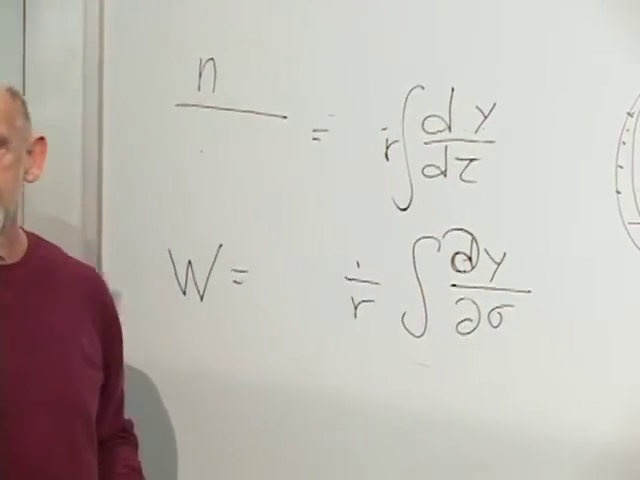
\includegraphics[width=0.72\textwidth]{lecture_10_figure_03.png}
  \medskip

  \begin{tikzpicture}[x=1cm,y=1cm,>=Latex]
    \draw[thick] (-4.0,0.3) circle (0.65);
    \draw[->,thick] (-4.55,0.58) arc (150:-145:0.65);
    \node at (-4.0,-0.65) {$w=+1$};
    \draw[thick] (-2.0,0.3) circle (0.65);
    \draw[->,thick] (-2.55,0.58) arc (150:-145:0.65);
    \node at (-2.0,-0.65) {$w=+1$};
    \node at (-3.0,0.3) {$+$};
    \draw[->,thick] (-1.0,0.3) -- (0.3,0.3);
    \draw[thick] (1.45,0.3) circle (0.78);
    \draw[thick] (1.45,0.3) circle (0.52);
    \draw[->,thick] (0.81,0.74) arc (145:-145:0.78);
    \node at (1.45,-0.78) {$w=+2$};
  \end{tikzpicture}
  \caption{Enrollamientos del mismo signo pueden reconectarse para formar una cuerda con el doble de enrollamiento. Cambia la conectividad, pero el enrollamiento total sigue siendo dos.}
  \lectureframe{00:16:40}
  \label{fig:l10-same-winding}
\end{figure}

Esta distinción se mantiene en todos los procesos permitidos. Un enrollamiento total de cien podría corresponder a una cuerda enrollada cien veces, a dos cuerdas enrolladas cincuenta veces cada una o a cien cuerdas enrolladas una vez. Las cuerdas pueden escindirse y unirse entre estas configuraciones, pero la suma con signo sigue siendo cien. La denotamos por \(w\in\mathbb Z\).

\section{Modos de momento y modos de enrollamiento}

La conservación por sí sola todavía no es dualidad. A continuación, compararemos las energías. Un estado que se mueve alrededor del círculo compacto tiene momento cuantizado
\begin{equation}
  p_Y=\frac{n}{R},
  \qquad n\in\mathbb Z.
  \label{eq:l10-compact-momentum}
\end{equation}
Para un estado en el que se puedan despreciar las demás contribuciones a la masa, el movimiento en la dimensión compacta contribuye \(E_{\rm mom}=|n|/R\). Los valores positivo y negativo de \(n\) indican sentidos opuestos del movimiento, mientras que la energía es positiva.

\begin{figure}[H]
  \centering
  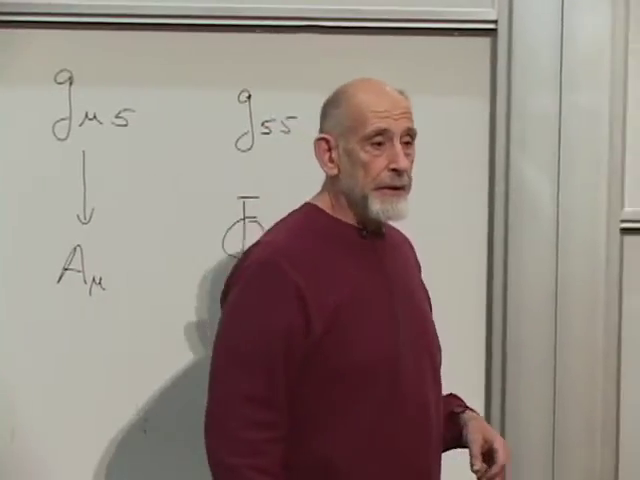
\includegraphics[width=0.72\textwidth]{lecture_10_figure_04.png}
  \caption{El número cuántico del momento compacto que aparece en la pizarra. En la clase, el momento se escribe esquemáticamente como una integral de la velocidad en la dirección compacta.}
  \lectureframe{00:21:30}
  \label{fig:l10-compact-momentum-board}
\end{figure}

Una cuerda enrollada \(|w|\) veces tiene longitud \(2\pi |w|R\). Con tensión fundamental de cuerda
\begin{equation}
  T_{\rm F}=\frac{1}{2\pi\alpha'},
\end{equation}
su energía de enrollamiento es
\begin{equation}
  E_{\rm wind}=T_{\rm F}(2\pi |w|R)
  =\frac{|w|R}{\alpha'}.
  \label{eq:l10-winding-energy}
\end{equation}
En las unidades de la clase \(\alpha'=1\), esto se reduce a \(E_{\rm wind}=|w|R\).

Las dos torres se comportan de manera opuesta cuando cambia el radio. Para \(R\gg
\sqrt{\alpha'}\), los niveles de momento están muy juntos y los de enrollamiento, muy separados. Para \(R\ll\sqrt{\alpha'}\), los niveles de momento están muy separados y los de enrollamiento, muy juntos.

\begin{figure}[H]
  \centering
  \begin{minipage}[t]{0.48\textwidth}
    \centering
    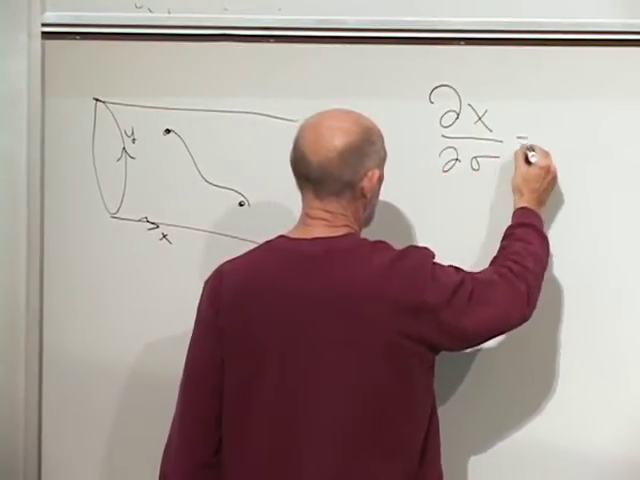
\includegraphics[width=\linewidth]{lecture_10_figure_05.png}
    \par\smallskip
    \textit{Radio compacto grande.}
  \end{minipage}\hfill
  \begin{minipage}[t]{0.48\textwidth}
    \centering
    \includegraphics[width=\linewidth]{lecture_10_figure_06.png}
    \par\smallskip
    \textit{Radio compacto pequeño.}
  \end{minipage}
  \caption{Las dos comparaciones espectrales de la pizarra. Las torres dispersas y densas intercambian sus papeles al invertir el radio.}
  \lectureframe{00:25:30--00:26:00}
  \label{fig:l10-dual-spectra-board}
\end{figure}

El esquema más claro es
\begin{figure}[H]
  \centering
  \begin{adjustbox}{max width=\linewidth}
  \begin{tikzpicture}[x=1cm,y=0.74cm,>=Latex]
    \node[font=\bfseries] at (-3.6,6.2) {$R\gg\sqrt{\alpha'}$};
    \draw[->] (-5.1,0) -- (-5.1,5.5) node[above] {$E$};
    \foreach \y in {0.4,1.0,1.6,2.2,2.8,3.4,4.0,4.6}
      \draw (-5.35,\y)--(-4.85,\y);
    \node[align=center] at (-4.25,5.15) {momentum\\dense};
    \draw[->] (-2.2,0) -- (-2.2,5.5) node[above] {$E$};
    \foreach \y in {0.4,2.4,4.4}
      \draw (-2.45,\y)--(-1.95,\y);
    \node[align=center] at (-1.35,5.15) {winding\\sparse};

    \node[font=\bfseries] at (3.6,6.2) {$R\ll\sqrt{\alpha'}$};
    \draw[->] (2.2,0) -- (2.2,5.5) node[above] {$E$};
    \foreach \y in {0.4,2.4,4.4}
      \draw (1.95,\y)--(2.45,\y);
    \node[align=center] at (3.05,5.15) {momentum\\sparse};
    \draw[->] (5.1,0) -- (5.1,5.5) node[above] {$E$};
    \foreach \y in {0.4,1.0,1.6,2.2,2.8,3.4,4.0,4.6}
      \draw (4.85,\y)--(5.35,\y);
    \node[align=center] at (5.95,5.15) {winding\\dense};
  \end{tikzpicture}
  \end{adjustbox}
  \caption{Reconstrucción del argumento basado en la separación entre niveles. El espectro completo de la cuerda no cambia cuando se intercambian el momento y el enrollamiento junto con \(R\leftrightarrow\alpha'/R\).}
  \label{fig:l10-dual-spectra-redraw}
\end{figure}

Supongamos que alguien recibe uno de estos espectros sin que le digan cómo se obtuvo. ¿Es la torre de niveles muy juntos el momento en un círculo grande o el enrollamiento en uno pequeño? El espectro por sí solo no permite saberlo. La teoría de cuerdas afirma algo más fuerte: tampoco los elementos de matriz de dispersión permiten distinguirlos. Las dos descripciones son exactamente equivalentes bajo
\begin{equation}
  n\longleftrightarrow w,
  \qquad
  R\longleftrightarrow \widetilde R=\frac{\alpha'}{R}.
  \label{eq:l10-radius-duality}
\end{equation}
El punto fijo es
\begin{equation}
  R=\sqrt{\alpha'},
  \label{eq:l10-self-dual-radius}
\end{equation}
o \(R=1\) en las unidades de la clase. En ese radio pueden volverse sin masa estados adicionales y se realza la simetría gauge.

\begin{classroomqa}
\audiencequestion{¿El enrollamiento es solo una conveniencia matemática para reescribir el espectro? \lecturetimestamp{00:27:33}}
\lecturerresponse{No. El enrollamiento etiqueta sectores reales del espacio de Hilbert de la cuerda cerrada, y esos sectores participan en las interacciones. La palabra ``dualidad'' significa que las descripciones en términos de momento y de enrollamiento son coordenadas distintas para una misma física, no que uno de los sectores sea un recurso mnemotécnico opcional para representar el otro.}
\end{classroomqa}

\begin{classroomqa}
\audiencequestion{¿Hay algún radio que se transforme en sí mismo?
\lecturetimestamp{00:27:58}}
\lecturerresponse{Sí. El valor autodual es
\(R=\sqrt{\alpha'}\), que corresponde a \(R=1\) en las unidades usadas en la pizarra. Allí coinciden las dos torres y el espectro presenta una simetría realzada.}
\end{classroomqa}

\section{La forma de la dualidad en la hoja de mundo}

El argumento espectral es sugerente, pero la hoja de mundo hace más precisa la correspondencia. En el gauge conforme, el momento conjugado a \(Y\) es proporcional a \(\partial_\tau Y\). Así, el momento compacto total tiene la forma
\begin{equation}
  P_Y=\frac{1}{2\pi\alpha'}
      \int_0^{2\pi}d\sigma\,\partial_\tau Y.
  \label{eq:l10-worldsheet-momentum}
\end{equation}
El número de enrollamiento es
\begin{equation}
  w=\frac{1}{2\pi R}
      \int_0^{2\pi}d\sigma\,\partial_\sigma Y
   =\frac{Y(2\pi)-Y(0)}{2\pi R}.
  \label{eq:l10-worldsheet-winding}
\end{equation}

\begin{classroomqa}
\audiencequestion{¿Por qué no se anula la integral de una derivada al recorrer la cuerda cerrada? \lecturetimestamp{00:32:33}}
\lecturerresponse{Porque \(Y\) es una coordenada periódica del espacio objetivo, no una función real univaluada en el círculo de coordenada \(\sigma\). El punto de la hoja de mundo \(\sigma=2\pi\) es el mismo que \(\sigma=0\), pero un levantamiento de la aplicación de inmersión a la recta recubridora cambia en \(2\pi wR\). La integral de \(\partial_\sigma Y\) mide ese desplazamiento.}
\end{classroomqa}

\begin{figure}[H]
  \centering
  \includegraphics[width=0.76\textwidth]{lecture_10_figure_07.png}
  \caption{Las integrales de momento y de enrollamiento, una vez completadas ambas expresiones en la pizarra. En la normalización de la clase se omiten los factores comunes \(2\pi\) y \(\alpha'\).}
  \lectureframe{00:33:25}
  \label{fig:l10-momentum-winding-integrals}
\end{figure}

Para una cuerda enrollada una vez,
\begin{equation}
  Y(\tau,\sigma+2\pi)=Y(\tau,\sigma)+2\pi R.
\end{equation}
Para un enrollamiento \(w\), el desplazamiento del lado derecho es \(2\pi wR\). La ecuación \eqref{eq:l10-worldsheet-winding} cuenta entonces exactamente el enrollamiento. Esta es la formulación precisa de la abreviatura de la pizarra \(w\sim R^{-1}\int
d\sigma\,\partial_\sigma Y\).

Por tanto, la formulación de la dualidad T en la hoja de mundo es
\begin{equation}
  \partial_\tau Y\longleftrightarrow
  \partial_\sigma \widetilde Y,
  \qquad
  \partial_\sigma Y\longleftrightarrow
  \partial_\tau \widetilde Y,
  \label{eq:l10-derivative-duality}
\end{equation}
donde el momento en \(Y\) se convierte en enrollamiento en la coordenada dual \(\widetilde Y\), y viceversa.

\begin{classroomqa}
\audiencequestion{¿Significa esto que las coordenadas de la hoja de mundo \(\tau\) y \(\sigma\) están relacionadas o se intercambian entre sí?
\lecturetimestamp{00:34:39}}
\lecturerresponse{No. La dualidad T transforma soluciones e intercambia derivadas específicas de la coordenada compacta del espacio objetivo. No identifica la coordenada temporal de la hoja de mundo con su coordenada espacial.}
\end{classroomqa}

\section{Por qué no se pueden evitar los estados con enrollamiento}

Cabe preguntarse por qué una cuerda llegaría a estar enrollada si existe un estado no enrollado. Una cuerda no elige su estado por preferencia. La energía suministrada en una colisión la estira. Una cuerda suficientemente energética y muy deformada puede reconectarse y dar lugar a dos cuerdas con enrollamientos opuestos. Su enrollamiento total sigue siendo cero, pero después de la escisión las dos cuerdas pueden separarse. Una de ellas puede alejarse mucho, y dejar a un observador con una cuerda aparentemente aislada y enrollada.

\begin{figure}[H]
  \centering
  \includegraphics[width=0.76\textwidth]{lecture_10_figure_08.png}
  \caption{Una configuración muy estirada con enrollamiento neto nulo, de la que pueden separarse cuerdas con enrollamientos opuestos tras la reconexión.}
  \lectureframe{00:36:15}
  \label{fig:l10-winding-pair-production}
\end{figure}

El umbral de energía viene determinado por la energía de enrollamiento. En un círculo grande, hace falta una energía de colisión elevada para estirar la cuerda lo suficiente como para que dé una vuelta alrededor de la dimensión compacta. Sin embargo, por encima del umbral no se puede prohibir la producción de pares de cuerdas enrolladas y anti-enrolladas--. La analogía es la producción de pares de electrones-- y positrones en colisiones de fotones. La carga eléctrica total sigue siendo cero, pero las partículas cargadas están presentes y pueden separarse. La conservación del enrollamiento funciona del mismo modo.

Esta analogía es más que una manera de hablar. El momento compacto y el enrollamiento se comportan como dos números cuánticos de carga distintos. En la descripción reducida correspondiente, las cargas del mismo signo se repelen y las de signo opuesto se atraen. Por tanto, debemos preguntar cuáles son los dos campos vectoriales que median esas fuerzas.

\section{Carga de momento a partir de la gravedad en cinco dimensiones}

Empecemos con la gravedad en cinco dimensiones. Sean los índices mayúsculos \(M,N\), que recorren las cuatro direcciones ordinarias del espacio-tiempo y la quinta dirección compacta. La métrica se descompone como
\begin{equation}
  G_{MN}\quad\longrightarrow\quad
  \bigl\{G_{\mu\nu},\,G_{\mu5},\,G_{55}\bigr\}.
  \label{eq:l10-metric-decomposition}
\end{equation}
La componente simétrica \(G_{5\mu}\) no contiene información nueva respecto de \(G_{\mu5}\).

\begin{figure}[H]
  \centering
  \includegraphics[width=0.74\textwidth]{lecture_10_figure_09.png}
  \caption{Los grupos independientes de componentes de la métrica en cinco dimensiones: \(G_{\mu\nu}\), \(G_{\mu5}\) y \(G_{55}\).}
  \lectureframe{00:44:05}
  \label{fig:l10-metric-components}
\end{figure}

Desde el punto de vista de cuatro dimensiones,
\begin{align}
  G_{\mu\nu} &\quad\hbox{is a spacetime metric},\\
  G_{\mu5} &\equiv A_\mu\quad\hbox{is a vector field},\\
  G_{55} &\equiv e^{2\varphi}\quad\hbox{is a scalar modulus}.
  \label{eq:l10-four-dimensional-fields}
\end{align}
El escalar \(\varphi\) mide el tamaño de la dimensión compacta. Puede variar suavemente a lo largo del espacio-tiempo ordinario, de modo que las ondas de \(\varphi\) son ondas en el radio de la quinta dimensión.

\begin{figure}[H]
  \centering
  \includegraphics[width=0.74\textwidth]{lecture_10_figure_10.png}
  \caption{En la pizarra se identifica \(G_{\mu5}\) con un vector \(A_\mu\) y \(G_{55}\) con un escalar \(\Phi\).}
  \lectureframe{00:47:40}
  \label{fig:l10-vector-and-radius-modulus}
\end{figure}

La fuente de una componente gravitatoria mixta es un flujo de momento mixto. En particular, el momento en la quinta dirección es fuente de \(G_{\mu5}\). Por tanto, un observador en cuatro dimensiones interpreta el entero \(n\) como una carga eléctrica acoplada a \(A_\mu\). Este es el mecanismo de Kaluza--Klein: lo que es momento en la geometría de dimensiones superiores se convierte en carga en la teoría de campos de dimensiones inferiores.

\editorialnote{En la clase se llama de manera informal \(G_{55}\) «``dilatón''» al escalar. En esta reducción es, en concreto, el módulo del radio. El dilatón de la cuerda en diez dimensiones, que controla el acoplamiento de cuerda, es un campo distinto, aunque ciertas combinaciones escalares de dimensiones inferiores pueden mezclarse al cambiar de marco y bajo dualidad.}

\begin{classroomqa}
\audiencequestion{¿El escalar \(\varphi\) es proporcional al entero de momento \(n\)? \lecturetimestamp{00:48:43}}
\lecturerresponse{No. El entero \(n\) etiqueta un estado cuantizado y actúa como carga. El escalar \(\varphi(x)\) es un campo continuo que determina el tamaño local de la compactificación. Puede variar de un lugar a otro; no es en sí mismo un entero.}
\end{classroomqa}

\section{El segundo campo vectorial y la carga de enrollamiento}

El enrollamiento también se comporta como una carga, pero no puede acoplarse al mismo vector de la misma manera. Para encontrar el segundo vector, volvamos a las primeras excitaciones de la cuerda cerrada. Una cuerda cerrada tiene modos de oscilador que se propagan hacia la izquierda y hacia la derecha. Los estados físicos satisfacen la condición de igualación de niveles: los niveles totales de excitación izquierda y derecha deben coincidir.

En la teoría bosónica, el estado no excitado es el taquión. Un solo oscilador de movimiento a la izquierda o a la derecha incumpliría la condición de igualación de niveles. Por tanto, el primer estado sin masa permitido contiene un oscilador de cada tipo,
\begin{equation}
  \alpha_{-1}^{I}\widetilde\alpha_{-1}^{J}\ket{0;k}.
  \label{eq:l10-first-massless-state}
\end{equation}
Los índices \(I,J\) recorren las direcciones espaciales transversales, incluida la dirección compacta. Si un índice corresponde a una dirección ordinaria y el otro a \(5\), hay dos estados de oscilador de tipo vectorial,
\begin{equation}
  \alpha_{-1}^{\mu}\widetilde\alpha_{-1}^{5}\ket{0;k},
  \qquad
  \alpha_{-1}^{5}\widetilde\alpha_{-1}^{\mu}\ket{0;k}.
  \label{eq:l10-two-vector-states}
\end{equation}

\begin{figure}[H]
  \centering
  \includegraphics[width=0.76\textwidth]{lecture_10_figure_11.png}
  \caption{Los dos órdenes de los osciladores izquierdo-- y derecho que dan lugar a estados vectoriales en cuatro dimensiones cuando una polarización apunta en la dirección compacta.}
  \lectureframe{00:58:20}
  \label{fig:l10-two-vector-states-board}
\end{figure}

Sus combinaciones simétrica y antisimétrica pertenecen a campos distintos del espacio-tiempo:
\begin{align}
  \alpha_{-1}^{(\mu}\widetilde\alpha_{-1}^{5)}\ket{0;k}
    &\longleftrightarrow G_{\mu5},\\
  \alpha_{-1}^{[\mu}\widetilde\alpha_{-1}^{5]}\ket{0;k}
    &\longleftrightarrow B_{\mu5}.
  \label{eq:l10-g-and-b-vectors}
\end{align}
El primero es el vector de Kaluza--Klein, cuya fuente es el momento compacto. El segundo desciende del campo antisimétrico de Kalb--Ramond y tiene como fuente el enrollamiento de la cuerda. Así, la teoría reducida contiene dos campos de tipo fotónico, uno para cada sector de carga.

Si ambos índices del oscilador apuntan en la dirección compacta, el estado es un escalar asociado al módulo de compactificación. Si ambos corresponden a direcciones transversales ordinarias, la parte simétrica sin traza es el gravitón, la parte antisimétrica es \(B_{\mu\nu}\) y la traza contribuye a un sector escalar.

\begin{classroomqa}
\audiencequestion{¿Cuál de estos estados es el singlete y cuál el triplete? \lecturetimestamp{01:00:21}}
\lecturerresponse{Esa clasificación no resulta útil aquí. Ambos estados mixtos se transforman como vectores en cuatro dimensiones. Su suma y su diferencia separan la polarización simétrica de la métrica de la polarización antisimétrica del campo \(B\). En cambio, el estado con dos índices compactos es un escalar en cuatro dimensiones.}
\end{classroomqa}

El diccionario completo al que llegamos antes de la pausa es
\begin{equation}
  \boxed{
  \begin{gathered}
    n\leftrightarrow w,
    \qquad
    R\leftrightarrow\dfrac{\alpha'}{R},\\
    \partial_\tau Y\leftrightarrow\partial_\sigma\widetilde Y,
    \qquad
    G_{\mu5}\leftrightarrow B_{\mu5}.
  \end{gathered}}
  \label{eq:l10-complete-t-duality-map}
\end{equation}

\begin{figure}[H]
  \centering
  \includegraphics[width=0.72\textwidth]{lecture_10_figure_12.png}
  \caption{Resumen de la correspondencia de dualidad T en la pizarra: se intercambian el momento y el enrollamiento, el radio y su inverso, las derivadas de la hoja de mundo y los dos campos vectoriales. El profesor oculta parcialmente la última línea, que por ello se incluye explícitamente en la ecuación \eqref{eq:l10-complete-t-duality-map}.}
  \lectureframe{01:02:20}
  \label{fig:l10-t-duality-map-board}
\end{figure}

Esta construcción no debe confundirse con la afirmación de que todos los campos enumerados ya se hayan identificado en el espectro observado de partículas. En este punto, es una consecuencia matemática de la teoría de cuerdas compactificada. Hay muchas propuestas para conectar estas estructuras con la fenomenología, pero ese no es el problema que resuelve esta clase.

\section{Las cuerdas abiertas cambian la pregunta}

Después de la pausa, retomamos el análisis con las cuerdas abiertas. Una cuerda cerrada puede tener un enrollamiento estable porque no tiene extremos por los que este pueda escabullirse. Una cuerda abierta tiene extremos y, por tanto, no posee un número de enrollamiento análogo protegido topológicamente. Sin embargo, la dualidad T es una simetría exacta de la teoría. ¿Qué hace esta simetría con una cuerda abierta?

Para un extremo que se mueve libremente, la variación de la acción de la cuerda da una condición de contorno de Neumann. En la geometría sencilla \((X,Y)\),
\begin{equation}
  \left.\partial_\sigma X\right|_{\partial\Sigma}=0,
  \qquad
  \left.\partial_\sigma Y\right|_{\partial\Sigma}=0.
  \label{eq:l10-neumann-boundary}
\end{equation}
La imagen mecánica es sencilla. Consideremos la cuerda como una cadena de elementos de masa cada vez más pequeños. Una fuerza tangencial no nula sobre el último elemento le produciría una aceleración que diverge cuando su masa tiende a cero. Por tanto, un extremo libre se ajusta hasta que la tensión neta en el extremo se anula. Otra persona podría sujetar el extremo fijo y ejercer la fuerza necesaria, pero entonces el extremo dejaría de ser libre.

\begin{figure}[H]
  \centering
  \includegraphics[width=0.76\textwidth]{lecture_10_figure_13.png}
  \caption{La cuerda abierta y sus condiciones de contorno de Neumann completas en los extremos, \(\partial_\sigma X=\partial_\sigma Y=0\).}
  \lectureframe{01:09:20}
  \label{fig:l10-neumann-board}
\end{figure}

Dualicemos ahora únicamente la coordenada compacta \(Y\). La coordenada no compacta \(X\) no cambia. La ecuación \eqref{eq:l10-derivative-duality} transforma la segunda condición de Neumann en
\begin{equation}
  \left.\partial_\tau\widetilde Y\right|_{\partial\Sigma}=0.
  \label{eq:l10-dirichlet-time-derivative}
\end{equation}
Por tanto, la posición del extremo en la dirección compacta dual no depende del tiempo,
\begin{equation}
  \left.\widetilde Y\right|_{\partial\Sigma}=Y_0.
  \label{eq:l10-dirichlet-boundary}
\end{equation}
Esta es una condición de contorno de Dirichlet.

\begin{figure}[H]
  \centering
  \includegraphics[width=0.76\textwidth]{lecture_10_figure_14.png}
  \medskip

  \begin{adjustbox}{max width=\linewidth}
  \begin{tikzpicture}[x=1cm,y=1cm,>=Latex]
    \node[align=center] at (-3.5,0.8)
      {Neumann\\\(\left.\partial_\sigma Y\right|_{\partial\Sigma}=0\)};
    \draw[->,thick] (-1.7,0.8) -- (1.3,0.8)
      node[midway,above] {$T_Y$};
    \node[align=center] at (3.4,0.8)
      {Dirichlet\\\(\left.\partial_\tau\widetilde Y\right|_{\partial\Sigma}=0\)};
    \node[align=center] at (3.4,-0.5)
      {\(\widetilde Y(\tau)=Y_0\) at each endpoint};
  \end{tikzpicture}
  \end{adjustbox}
  \caption{La condición de contorno completa del extremo dual en la pizarra y su reconstrucción lógica clara. La dualidad T transforma la libertad en la dirección compacta en una posición fija del extremo en la dirección dual.}
  \lectureframe{01:12:35}
  \label{fig:l10-neumann-to-dirichlet}
\end{figure}

\begin{classroomqa}
\audiencequestion{¿Por qué significa la condición dual que el extremo está fijo? \lecturetimestamp{01:12:39}}
\lecturerresponse{Porque \(\partial_\tau\widetilde Y=0\) es una velocidad nula en la dirección dualizada. Dondequiera que comience el extremo en \(\widetilde Y\), allí permanecerá. Sus coordenadas en las direcciones paralelas a las no dualizadas siguen siendo libres.}
\end{classroomqa}

\section{El objeto que sujeta el extremo es una D-brana}

Si un extremo está fijo, algo debe poder mantenerlo allí. Por tanto, la dualidad T exacta exige un objeto nuevo sobre el que puedan terminar las cuerdas abiertas. Ese objeto es una D-brana. La letra \(D\) representa Dirichlet, no la dimensión del objeto. En el aparte histórico de la clase se señala que estos objetos podrían haberse llamado en honor de Joseph Polchinski, cuyo análisis hizo innegable su papel dinámico; sin embargo, el término ya establecido «``p-brana''» hacía de Dirichlet el nombre más natural.

Una brana de tipo \(p\) tiene \(p\) dimensiones espaciales. Una cuerda es una brana de una dimensión, una membrana es una brana de dos dimensiones y un objeto extenso tridimensional es una brana de tres dimensiones. Una D\(p\)-brana es una brana de tipo \(p\) en la que los extremos de las cuerdas fundamentales satisfacen condiciones de Dirichlet en las direcciones transversales y condiciones de Neumann en las direcciones tangentes a la brana.

Nada en el argumento de dualidad señala un valor particular de \(Y_0\); por tanto, la D-brana no puede ser un soporte rígido clavado en un punto preferente del universo. Debe poder moverse. La relatividad también prohíbe los cuerpos extensos absolutamente rígidos, así que una D-brana puede fluctuar y curvarse. La brana plana y sencilla dibujada en la pizarra es su configuración de equilibrio, no una restricción a su dinámica.

\begin{classroomqa}
\audiencequestion{¿Deben los dos extremos de una cuerda abierta tener el mismo valor fijo de la coordenada dual? \lecturetimestamp{01:14:55}}
\lecturerresponse{No necesariamente. Ambos extremos pueden estar sobre la misma D-brana, en cuyo caso comparten la posición transversal de esa brana. También pueden estar sobre dos D-branas distintas, situadas en posiciones transversales diferentes; entonces la cuerda se extiende entre ellas. La propia brana puede fluctuar y curvarse, de modo que el lugar geométrico de los extremos no tiene por qué seguir siendo un plano perfectamente llano.}
\end{classroomqa}

\section{Cómo contar las dimensiones de una D-brana}

La teoría de supercuerdas en diez dimensiones tiene nueve dimensiones espaciales. Supongamos que la dualidad T impone una condición de Dirichlet en una dirección espacial. El extremo aún puede moverse libremente en las otras ocho, de modo que su lugar geométrico permitido es una D8-brana de ocho dimensiones. Cada condición de Dirichlet independiente adicional elimina una dirección de movimiento del extremo. Si se fijan \(k\) coordenadas espaciales, entonces
\begin{equation}
  p=9-k.
  \label{eq:l10-dp-counting}
\end{equation}

La mesa ilustra la misma cuenta en tres dimensiones. Si se fija la coordenada vertical, la yema de un dedo puede moverse sobre una mesa bidimensional. Si se fija una segunda coordenada, solo puede moverse a lo largo de una línea. Si se fijan las tres, queda confinada a un punto.

\begin{figure}[H]
  \centering
  \begin{adjustbox}{max width=\linewidth}
  \begin{tikzpicture}[x=1.05cm,y=1cm,>=Latex]
    \draw[fill=blue!8] (-5.5,-0.7) -- (-2.5,-0.7) -- (-1.7,0.2)
      -- (-4.7,0.2) -- cycle;
    \node at (-3.6,-1.15) {one constraint: sheet};
    \draw[very thick,blue!60!black] (-0.9,-0.25) -- (1.3,-0.25);
    \node at (0.2,-1.15) {two constraints: line};
    \fill[blue!70!black] (4.1,-0.25) circle (0.09);
    \node at (4.1,-1.15) {three constraints: point};
    \draw[->] (-1.45,0.95) -- (-0.75,0.95);
    \draw[->] (2.25,0.95) -- (2.95,0.95);
    \node at (0.35,1.35) {each Dirichlet condition lowers \(p\) by one};
  \end{tikzpicture}
  \end{adjustbox}
  \caption{El argumento de recuento de dimensiones ilustrado en la mesa. Una D\(p\)-brana es el lugar geométrico en el que los extremos pueden moverse libremente.}
  \label{fig:l10-dp-counting-redraw}
\end{figure}

Las dualidades sucesivas generan D8-, D7-, D6-branas y así sucesivamente, hasta llegar a una D0-brana, que es puntual en el espacio. Si no se fija ninguna dirección espacial, una D9-brana ocupa las nueve dimensiones espaciales y las cuerdas abiertas ordinarias pueden moverse por todas partes. En la clase se mencionan brevemente las D\((-1)\)-branas; están localizadas en el espacio-tiempo euclídeo y se comportan como instantones, no como partículas ordinarias que se propagan en el tiempo.

\editorialnote{La escala de dimensiones es una afirmación sobre las teorías de tipo II consideradas en conjunto. Las D\(p\)-branas BPS estables tienen valor par de \(p\) en la teoría de tipo IIA y valor impar de \(p\) en la teoría de tipo IIB. La dualidad T a lo largo de un círculo cambia \(p\) en una unidad e intercambia simultáneamente las teorías de tipo IIA y de tipo IIB.}

\begin{classroomqa}
\audiencequestion{Si solo hay seis dimensiones compactas, ¿debería empezar el recuento restando a partir de seis en lugar de nueve? \lecturetimestamp{01:20:49}}
\lecturerresponse{La derivación elemental aplica la dualidad T a las direcciones compactas, pero el círculo dual se vuelve arbitrariamente grande cuando el círculo original se hace arbitrariamente pequeño. En ese límite, es efectivamente no compacto. Por tanto, las branas resultantes pueden extenderse a lo largo de direcciones o ser transversales a ellas, aunque a escalas accesibles parezcan no compactas. La dimensión \(p\) cuenta todas las direcciones espaciales tangentes a la brana, no solo las compactas que se usan en una derivación concreta.}
\end{classroomqa}

Una D0-brana es un nuevo tipo de partícula. Una cuerda abierta puede ir de una D0-brana a otra, regresar a la misma D0-brana o extenderse hacia una brana muy distante. Si uno de sus extremos llegara literalmente al infinito espacial, la cuerda tendría longitud infinita y, por tanto, energía infinita; así que la opción físicamente útil consiste en situar el otro extremo en otro objeto.

El siguiente caso, una D1-brana, también tiene forma de cuerda, pero no es la cuerda fundamental con la que empezamos. Puede curvarse y cerrarse sobre sí misma, y las cuerdas fundamentales pueden terminar en ella. Su tensión depende de manera distinta del acoplamiento de cuerdas:
\begin{equation}
  T_{\rm D1}=\frac{1}{2\pi\alpha' g_s},
  \qquad
  T_{\rm F1}=\frac{1}{2\pi\alpha'}.
  \label{eq:l10-dstring-tension}
\end{equation}
A acoplamiento débil \(g_s\ll1\), la cuerda D es mucho más pesada que la cuerda fundamental, lo que explica por qué aparece primero como un ancla masiva.

\begin{figure}[H]
  \centering
  \includegraphics[width=0.76\textwidth]{lecture_10_figure_15.png}
  \caption{La D1-brana de la pizarra: un objeto unidimensional flexible, distinto de las cuerdas fundamentales que pueden terminar en ella.}
  \lectureframe{01:24:20}
  \label{fig:l10-d1-brane}
\end{figure}

\begin{classroomqa}
\audiencequestion{¿Actúa la dualidad T sobre las D-branas además de sobre las cuerdas? \lecturetimestamp{01:25:35}}
\lecturerresponse{Sí. Una dualidad T paralela a una D\(p\)-brana reduce su dimensión a D\((p-1)\), mientras que una dualidad T transversal a ella aumenta su dimensión a D\((p+1)\). Las branas forman parte del diccionario de dualidad; no son soportes externos que esta deje intactos.}
\end{classroomqa}

\begin{classroomqa}
\audiencequestion{¿Pueden seguir siendo compactas las direcciones tangentes a una brana?
\lecturetimestamp{01:27:25}}
\lecturerresponse{Sí. ``Tangencial'' y ``compacta'' responden a preguntas distintas. Una dirección puede extenderse a lo largo de la brana y aun así cerrarse formando un círculo; también puede ser no compacta. Para el extremo, lo que importa es si la condición de contorno en esa dirección es de Neumann o de Dirichlet.}
\end{classroomqa}

Una D2-brana es una lámina similar a una membrana. Una D3-brana tiene tres dimensiones espaciales. En un espacio-tiempo genuinamente de dimensiones superiores, una D3-brana es un subespacio tridimensional, no todo el espacio, aunque los observadores confinados a ella puedan experimentarla como la totalidad de su mundo espacial.

\begin{figure}[H]
  \centering
  \includegraphics[width=0.76\textwidth]{lecture_10_figure_16.png}
  \caption{Una D2-brana representada como una lámina sobre la que pueden moverse los extremos de las cuerdas.}
  \lectureframe{01:27:55}
  \label{fig:l10-d2-brane}
\end{figure}

La derivación que se presenta aquí es deliberadamente esquemática. Por sí sola, no demuestra que la teoría de cuerdas describa la naturaleza. Sin embargo, dentro de la teoría de cuerdas hay numerosas comprobaciones de consistencia: las dualidades, los cálculos cuánticos y los resultados matemáticos apuntan a que las D-branas son objetos dinámicos reales.

\section{Las cuerdas abiertas se convierten en campos en una brana}

Tomemos una D2-brana vacía y coloquemos en ella cuerdas abiertas cortas. Cada extremo está confinado a la lámina, de modo que toda la excitación de baja energía se mueve a lo largo de ella. Dos cuerdas orientadas cuyos extremos adyacentes tengan flechas compatibles pueden unirse. Más adelante, la cuerda resultante puede volver a dividirse. Interpretados como historias de partículas, estos procesos son los vértices de los diagramas de Feynman: entran dos partículas, se propaga una excitación intermedia y salen dos partículas.

\begin{figure}[H]
  \centering
  \includegraphics[width=0.76\textwidth]{lecture_10_figure_17.png}
  \caption{Cuerdas abiertas orientadas sobre una D2-brana que se unen mediante extremos compatibles. A baja energía, el proceso se interpreta como una interacción de teoría de campos en la brana.}
  \lectureframe{01:29:55}
  \label{fig:l10-open-strings-on-brane}
\end{figure}

A energías muy inferiores a la escala de cuerdas, no se excita la torre de modos vibracionales internos. El estado restante de cuerda abierta, que no tiene masa, es un campo vectorial en el volumen de mundo de la brana. Para una sola brana, se trata de un campo de gauge abeliano \(U(1)\), análogo en la brana al electromagnetismo. El campo no se propaga por todo el volumen de diez dimensiones; sus cuantos son cuerdas abiertas cuyos extremos los mantienen en la brana.

\section{Una pila de branas produce color no abeliano}

Ahora coloquemos varias branas paralelas cerca unas de otras. Para tres branas, llamémoslas Roja, Verde y Azul. Una cuerda orientada tiene un par ordenado de etiquetas en sus extremos: puede ir de Roja a Verde, de Verde a Azul, de Roja a Roja, etcétera. Con \(N\) branas, los estados de cuerda abierta sin masa pueden organizarse como una matriz \(N\times N\)
\begin{equation}
  A_\mu{}^{i}{}_{j},
  \qquad i,j=1,\ldots,N.
  \label{eq:l10-chan-paton-matrix}
\end{equation}
Estas son las etiquetas de Chan--Paton de una teoría de gauge \(U(N)\).

\begin{figure}[H]
  \centering
  \includegraphics[width=0.76\textwidth]{lecture_10_figure_18.png}
  \medskip

  \begin{adjustbox}{max width=\linewidth}
  \begin{tikzpicture}[x=1cm,y=1cm,>=Latex]
    \draw[very thick,red!70!black] (-4.8,2.0)--(4.8,2.0);
    \draw[very thick,green!55!black] (-4.8,0.8)--(4.8,0.8);
    \draw[very thick,blue!70!black] (-4.8,-0.4)--(4.8,-0.4);
    \node[left] at (-4.8,2.0) {Red};
    \node[left] at (-4.8,0.8) {Green};
    \node[left] at (-4.8,-0.4) {Blue};
    \draw[->,thick] (-3.4,2.0) .. controls (-2.8,1.35) and (-2.3,1.15)
      .. (-1.7,0.8);
    \node at (-2.7,1.05) {$R\!G$};
    \draw[->,thick] (-0.6,0.8) .. controls (0.0,0.25) and (0.6,-0.05)
      .. (1.2,-0.4);
    \node at (0.1,0.0) {$G\!B$};
    \draw[->,thick] (2.1,2.0) .. controls (2.9,2.55) and (3.8,2.55)
      .. (4.3,2.0);
    \node at (3.2,2.65) {$R\!R$};
  \end{tikzpicture}
  \end{adjustbox}
  \caption{Tres branas paralelas en la pizarra y una reconstrucción clara de las etiquetas ordenadas de los extremos que llevan las cuerdas que las conectan.}
  \lectureframe{01:33:15}
  \label{fig:l10-three-brane-stack}
\end{figure}

\begin{classroomqa}
\audiencequestion{¿Puede realmente una cuerda ir de la brana Roja a la brana Verde sin que se lo impidan los otros trazos del dibujo? \lecturetimestamp{01:35:07}}
\lecturerresponse{Sí. Las branas están inmersas en un espacio de dimensiones superiores. El dibujo bidimensional de la pizarra es solo una proyección, así que una cuerda puede pasar alrededor de otra línea proyectada desplazándose en una dirección transversal.}
\end{classroomqa}

\begin{classroomqa}
\audiencequestion{¿Es necesario que una cuerda Roja--Verde se combine con una cuerda Verde--Azul para convertirse en una Roja--Azul? \lecturetimestamp{01:35:39}}
\lecturerresponse{Esa es la regla básica de unión local. Los extremos compatibles se encuentran y los dos segmentos se convierten en una sola cuerda cuyos extremos libres conservan las etiquetas Roja y Azul. Los procesos más elaborados se construyen repitiendo la misma operación.}
\end{classroomqa}

La regla de unión es la multiplicación de matrices llevada a la geometría. Una cuerda Roja--Verde puede unirse con una cuerda Verde--Azul porque el extremo Verde de una es compatible con el extremo Verde de la otra. El resultado es una cuerda Roja--Azul:
\begin{equation}
  (R,G)\circ(G,B)\longrightarrow(R,B).
  \label{eq:l10-color-composition}
\end{equation}
El índice repetido se contrae y desaparece internamente. Esta es la misma estructura de índices que aparece en un vértice de interacción de Yang--Mills.

\begin{figure}[H]
  \centering
  \includegraphics[width=0.76\textwidth]{lecture_10_figure_19.png}
  \caption{Unión de cuerdas abiertas en una pila. La orientación de los extremos impone la misma composición de índices ordenados que se usa en los campos de gauge no abelianos.}
  \lectureframe{01:36:30}
  \label{fig:l10-color-joining-board}
\end{figure}

Para tres branas coincidentes, el grupo de gauge completo de las cuerdas abiertas es \(U(3)\), con nueve estados vectoriales. Su álgebra se descompone así:
\begin{equation}
  \mathfrak u(3)=\mathfrak{su}(3)\oplus\mathfrak u(1).
  \label{eq:l10-u3-decomposition}
\end{equation}
Las ocho combinaciones sin traza tienen la estructura de color de los gluones de la QCD, mientras que el \(U(1)\) diagonal del centro de masas es un campo abeliano independiente.

\editorialnote{La clase describe una de las nueve combinaciones de pares de color como algo que puede desprenderse y desaparecer, dejando así ocho gluones. La afirmación precisa sobre las D-branas es que una pila de tres branas coincidentes da \(U(3)\), no solo \(SU(3)\). Para obtener el octete de la QCD hay que separar, proyectar o desacoplar de algún otro modo el \(U(1)\) diagonal. La imagen de la clase motiva correctamente los índices de color ordenados, pero no constituye una derivación completa de la QCD.}

La materia similar a los quarks lleva un solo índice de color. En la imagen de las branas, la representa una cuerda con un extremo en la pila de color y el otro en una brana distinta y distante. Respecto de la pila de color, solo un extremo es visible como etiqueta de color. Al invertir la orientación se obtiene la antipartícula. Una cuerda similar a un quark y otra similar a un antiquark, con extremos compatibles, pueden unirse y separarse de la pila de color; dos cuerdas orientadas de la misma manera y similares a quarks no pueden aniquilarse de ese modo.

Las teorías resultantes de baja energía suelen ser teorías supersimétricas de Yang--Mills, con materia adicional determinada por las branas y sus intersecciones. Se parecen lo bastante a la QCD como para esclarecer la dinámica no abeliana, pero no son automáticamente el modelo estándar. Con una sola brana, la misma construcción se reduce a una teoría \(U(1)\): las cuerdas cortas entre branas--branas son similares a fotones, mientras que las cuerdas orientadas que llegan a un segundo sector desempeñan el papel de las cargas eléctricas positivas y negativas.

\section{Las cuerdas D terminan como monopolos magnéticos}

Ahora hay dos tipos de objetos con forma de cuerda en este relato. La cuerda fundamental, o cuerda F, transporta flujo eléctrico en una D3-brana. La D1-brana, o cuerda D, es mucho más pesada a acoplamiento débil. Una cuerda D también puede terminar en una D3-brana. Su extremo no tiene carga eléctrica respecto del campo de gauge del volumen de mundo; tiene carga magnética. Desde la perspectiva de los observadores en la D3-brana, el extremo es un monopolo magnético.

\begin{figure}[H]
  \centering
  \includegraphics[width=0.76\textwidth]{lecture_10_figure_20.png}
  \medskip

  \begin{adjustbox}{max width=\linewidth}
  \begin{tikzpicture}[x=1cm,y=1cm,>=Latex]
    \draw[fill=blue!7] (-3.8,-0.5)--(2.6,-0.5)--(3.6,0.35)--(-2.8,0.35)--cycle;
    \node at (2.25,-0.95) {D3-brane};
    \draw[very thick,red!70!black] (0.0,3.0)--(0.0,0.0);
    \fill[black] (0.0,0.0) circle (0.08);
    \node[right] at (0.15,2.1) {D-string};
    \foreach \a in {25,65,115,155} {
      \draw[->,blue!65!black] (0.0,0.0)--({1.25*cos(\a)},{0.65*sin(\a)});
    }
    \node[align=center] at (4.8,1.7) {magnetic flux\\on the D3 worldvolume};
    \draw[->] (3.7,1.35)--(1.05,0.45);
  \end{tikzpicture}
  \end{adjustbox}
  \caption{La construcción del extremo en la pizarra y su interpretación clara. Una cuerda D que termina en una D3-brana aparece como un monopolo magnético para la teoría de gauge del volumen de mundo.}
  \lectureframe{01:41:30}
  \label{fig:l10-dstring-monopole}
\end{figure}

La jerarquía de masas también tiene la forma cualitativa adecuada. Como la tensión de la cuerda D lleva un factor \(1/g_s\), su extremo es mucho más pesado que una excitación eléctrica ordinaria a acoplamiento débil. La relación eléctrica/magnética entre los extremos de las cuerdas F y D forma parte de la estructura más amplia de dualidad de la teoría de cuerdas de tipo IIB.

\begin{classroomqa}
\audiencequestion{¿Es neutro el extremo de la cuerda D?
\lecturetimestamp{01:42:19}}
\lecturerresponse{Es neutro respecto de la carga eléctrica que transporta el extremo de una cuerda fundamental, pero no carece de carga. Tiene carga magnética y, por tanto, es un monopolo en la teoría de gauge de la D3-brana.}
\end{classroomqa}

\section{Qué afirma y qué no afirma esta construcción}

El recorrido desde la dualidad T hasta las branas se fue construyendo a lo largo de décadas, no en un solo cálculo. Una teoría propuesta inicialmente para describir los hadrones se convirtió en una candidata a teoría de la gravedad cuántica. Sus dualidades hicieron luego necesarias las D-branas en el espectro, y las teorías de gauge reaparecieron como la dinámica de baja energía de las cuerdas que terminan en esas branas. En ese sentido, el tema completó un ciclo.

Las D-branas y otras construcciones duales relacionadas se han convertido en herramientas poderosas para estudiar teorías de gauge supersimétricas, sistemas de acoplamiento fuerte y conexiones entre la gravedad y la teoría de campos. También han contribuido a modelos de fluidos y plasmas mediante la dualidad gauge/gravedad. Este éxito no equivale a derivar directamente el espectro de partículas observado. Todavía hay que elegir la geometría de compactificación, la configuración de branas, la ruptura de supersimetría y muchos otros ingredientes.

\begin{classroomqa}
\audiencequestion{¿Qué determina qué dimensión compacta se dualiza?
\lecturetimestamp{01:44:59}}
\lecturerresponse{Matemáticamente, se puede dualizar cualquier dirección compacta para la que exista la simetría necesaria, eligiendo la descripción más conveniente. Físicamente, las orientaciones de las branas y los datos de compactificación que se realizan en un estado concreto vienen determinados por la historia y la dinámica de ese estado.}
\end{classroomqa}

\begin{classroomqa}
\audiencequestion{¿Qué brana sirve de soporte para la construcción del monopolo?
\lecturetimestamp{01:45:21}}
\lecturerresponse{El mundo que experimenta la teoría de gauge es una D3-brana. La cuerda D se extiende en una dirección transversal y termina en esa D3-brana; su extremo es el monopolo que se observa en las tres dimensiones espaciales de la brana.}
\end{classroomqa}

\begin{classroomqa}
\audiencequestion{¿También tienen orientación las cuerdas D?
\lecturetimestamp{01:45:55}}
\lecturerresponse{Sí. Invertir la orientación de una cuerda D invierte la carga correspondiente. Las dos orientaciones de los extremos distinguen el monopolo del antimonopolo, del mismo modo que la orientación distingue la carga eléctrica en los extremos de las cuerdas fundamentales.}
\end{classroomqa}

\begin{classroomqa}
\audiencequestion{¿Puede esta imagen toroidal sencilla dar cuenta de la asimetría izquierda--derecha de la física de partículas quiral?
\lecturetimestamp{01:46:05}}
\lecturerresponse{Por sí sola, no. Un toro plano es demasiado simétrico. Los espectros quirales requieren más estructura, como intersecciones asimétricas de branas, proyecciones de orbifold o compactificaciones en geometrías de Calabi--Yau adecuadas. La teoría de cuerdas cuenta con mecanismos para obtener quiralidad, pero quedan fuera de esta construcción elemental de dualidad T.}
\end{classroomqa}

Hemos seguido una simetría a través de cuatro manifestaciones concretas: un intercambio de espectros, un intercambio de derivadas de la hoja de mundo, un intercambio de campos del espacio-tiempo y, por último, un intercambio de condiciones de contorno en los extremos. Esta última manifestación es la decisiva. Convierte una equivalencia matemática en el descubrimiento de las D-branas y transforma la dinámica de las cuerdas abiertas en una teoría de gauge sobre sus volúmenes de mundo. En ese punto, en palabras de Susskind, la clase ha agotado su tiempo, su energía y su momento.
\end{document}